

%\documentclass{report}
\documentclass[a4paper]{scrreprt}
\usepackage{typearea}
\areaset[1cm]{158mm}{234mm}

\def\manifemrelease{22.**}
\def\manualversion{22.**}
\let\production 0
\includeonly{manual-cap-07}
% \usepackage{showkeys}

\usepackage{xcolor}
\usepackage{graphicx}
\usepackage{psfrag}
\usepackage{caption}
\usepackage{subcaption}

\usepackage{fancybox}
\usepackage{fancyvrb}
% \renewcommand\VerbatimFont{\tiny\tt}

\usepackage{amssymb}
\usepackage{indentfirst}

% \usepackage{geometry}
% \geometry { a4paper  }

% \usepackage{lmodern}
% \ttfamily\fontseries{l}\selectfont light text
% \ttfamily\fontseries{m}\selectfont normal text
% \fontseries{b}\selectfont bold text

% \def\numb #1 {}
\def\numb{}
\usepackage{tocbasic}
\DeclareTOCStyleEntry[dynindent=on]{default}{section}

\newcommand\ManiFEM{\leavevmode\hbox{
\includegraphics[width=13mm]{manifem-large}}}
\newcommand\maniFEM{\leavevmode\hbox{
\includegraphics[width=13mm]{manifem-small}}}

\definecolor{manif}{rgb}{0., 0., 0.5}
\definecolor{tag}{rgb}{0.07, 0.07, 0.3}
\definecolor{tag}{rgb}{0.12, 0.12, 0.4}
\definecolor{coment}{rgb}{0.3, 0.3, 0.3}
\definecolor{nova}{rgb}{0.55, 0., 0.2}
\definecolor{incl}{rgb}{0.3, 0.2, 0.1}
\definecolor{string}{rgb}{0.1, 0.25, 0.}
\definecolor{textindraw}{rgb}{0., 0.37, 0.}
\definecolor{numero}{rgb}{0.6, 0.3, 0.}
% \definecolor{nova}{rgb}{0., 0., 0.8}
% \definecolor{coment}{rgb}{0.5, 0.5, 0.5}
% \definecolor{manif}{rgb}{0.6, 0.1, 0.1}
% \definecolor{numero}{rgb}{0.7, 0.4, 0.}
\newcommand\azul[1]{\textcolor{nova}{#1}}
\newcommand\cinza[1]{\textcolor{coment}{#1}}
\newcommand\verm[1]{\textcolor{manif}{#1}}
\newcommand\verde[1]{\textcolor{string}{#1}}
\newcommand\laranja[1]{\textcolor{numero}{#1}}

\renewcommand\tt{\normalfont\ttfamily}



\title{
\includegraphics[width=12cm]{manifem-grey-capital.eps}}
\subtitle{USER MANUAL}
\author{Cristian Barbarosie and Anca-Maria Toader}
\date{\small version of this manual: \manualversion\\ documents \maniFEM\ release \manifemrelease}


%%%%%%%%%%%%%%%%%%%%%%%%%%%%%%%%%%%%%%%%%%%%%%%%%%%%%%%%%%%%%%%%%%%%%%%%%%%%%%%%%%%%%%%%%%%%%%%

\begin{document}

\begin{titlepage}
\maketitle
\end{titlepage}

%%%%%%%%%%%%%%%%%%%%%%%%%%%%%%%%%%%%%%%%%%%%%%%%%%%%%%%%%%%%%%%%%%%%%%%%%%%%%%%%%%%%%%%%%%%%%%%

\chapter*{}

This document describes \maniFEM, a {\tt C++} library for solving partial differential equations
through the finite element method.
The name comes from ``finite elements on manifolds''. 
{\ManiFEM} was designed with the goal of coping with very general meshes,
in particular meshes on Riemannian manifolds, even manifolds which cannot be embedded
in $ {\mathbb R}^3 $, like the torus $ {\mathbb R}^2/{\mathbb Z}^2 $.
Also, {\maniFEM} was written with the goal of being conceptually clear
and easy to read.
We hope it will prove particularly useful for people who want fine control on the mesh,
e.g.\ for implementing their own meshing or remeshing algorithms.

{\ManiFEM} is just a collection of {\tt C++} classes.
It has no user-friendly interface nor graphic capabilities.
The user should have some understanding of programming and of {\tt C++}.
However, {\maniFEM} can be used at a basic level by people with no deep knowledge of
{\tt C++}.
A gallery of examples is available at {\small\tt http://manifem.rd.ciencias.ulisboa.pt/gallery.html}.
At the end of section \ref{\numb section 1}, you can find three lists showing
{\maniFEM}'s competitors, as well as strong and weak points.

In its current version, release \manifemrelease, {\maniFEM} works well for mesh generation,
including meshes on quotient manifolds.
{\ManiFEM} deals well with one-dimensional meshes (including curves in $ {\mathbb R}^2 $ and
$ {\mathbb R}^3 $) and two-dimensional meshes (including surfaces in $ {\mathbb R}^3 $);
three-dimensional meshing is limited to cubic cells
(paragraphs \ref{\numb section 1.\numb parag 7} and \ref{\numb section 2.\numb parag 12}).
It is possible to build meshes with large variations in the element size;
anisotropic Riemann metrics are object of current work.
Lagrange finite elements of degree one and two are implemented for triangular and quadrangular
cells; many other types of finite elements are still to be implemented.
In the future, variational formulations will be implemented as {\tt C++} objects,
thus allowing for compact and elegant code.
A changelog is included at the end of this manual, before the index.
To check which version of {\maniFEM} is installed in your computer,
see at the beginning of the file {\small\tt maniFEM.h}.

A component of \maniFEM, {\small\tt MetricTree}, can be used independently.
It is a generalization of quad-trees for metric spaces.
See paragraph \ref{\numb section 12.\numb parag 10}.

Some examples use the {\small\tt Eigen} library for  storing matrices and solving systems of
linear equations, see {\small\tt http://eigen.tuxfamily.org/index.php?title=Main\_\,Page}.
Many drawings in this manual have been produced by {\small\tt gmsh}, see
{\small\tt http://gmsh.info/}

{\ManiFEM} is being developed by Cristian Barbarosie,%
\footnote {\small\tt cristian.barbarosie@gmail.com}
S\'ergio Lopes and Anca-Maria Toader.
% Their work is supported by National Funding from FCT -- Funda\c c\~ao para a Ci\^encia e a
% Tecnologia (Portugal), through Faculdade de Ci\^encias da Universidade de Lisboa and
% Centro de Matem\'atica, Aplica\c c\~oes Fundamentais e Investiga\c c\~ao Operacional.%
% \footnote{project UID/MAT/04561/2020}

{\ManiFEM} is free software; it is copyrighted by Cristian Barbarosie
under the GNU Lesser General Public Licence.

The home page of {\maniFEM} is {\small\tt http://manifem.rd.ciencias.ulisboa.pt}
(where this manual can be found).

To use \maniFEM, visit {\small\tt https://github.com/cristian-barbarosie/manifem},
choose a release and download all files to some directory in your computer.
Current code may be unstable, releases are stable.
You can then run the examples in this manual :
just {\small\tt make run-\ref{\numb section 1.\numb parag 1}}
for the example in paragraph \ref{\numb section 1.\numb parag 1},
{\small\tt make run-\ref{\numb section 2.\numb parag 6}}
for the example in paragraph \ref{\numb section 2.\numb parag 6}, and so on.
Paragraph \ref{\numb section 11.\numb parag 16} gives more details.
\vfil\eject


\section*{Structure of this manual}

This manual is divided in sections describing {\maniFEM} with increasing degree of technical
detail.
Sections \ref{\numb section 1} to \ref{\numb section 8} should be accessible to readers
who have some knowledge of {\tt C++} but are not necessarily experts in {\tt C++} programming.
Sections \ref{\numb section 9} and \ref{\numb section 10} should be useful for users
who want finer control on the mesh, e.g.\ for implementing their own remeshing algorithms.
Sections \ref{\numb section 11} and \ref{\numb section 12} give technical details,
mainly for those interested in developing and extending \maniFEM.

\subparagraph*{\ref{\numb section 1} \ General description}
A quick overview of \maniFEM's capabilities.

\subparagraph*{\ref{\numb section 2} \ Meshes and manifolds; patchwork}
Shows how to build meshes by joining simple shapes, like patches, some of them on manifolds.

\subparagraph*{\ref{\numb section 3} \ Progressive mesh generation; knitting}
Shows how to build meshes starting from their boundary alone, some of them on manifolds.

\subparagraph*{\ref{\numb section 4} \ \cinza{[empty]}}

\subparagraph*{\ref{\numb section 5} \ Fields, functions and variational formulations}
Some details about functions, a lot of work to do.

\subparagraph*{\ref{\numb section 6} \ Finite elements and integrators}
Shows examples of finite element computations, still rudimentary.

\subparagraph*{\ref{\numb section 7} \ Quotient manifolds}
Describes meshes on quotient manifolds.

\subparagraph*{\ref{\numb section 8} \ Miscellanea}
Gives informations which do not fit in other sections of the manual.

\subparagraph*{\ref{\numb section 9} \ Cells, meshes, iterators}
Gives details about neighbourhood relations between cells in a mesh, orientation and iterators.

\subparagraph*{\ref{\numb section 10} \ Remeshing}
Some simple examples showing how to manipulate a mesh.

\subparagraph*{\ref{\numb section 11} \ Technical details}
Various implementation detais, programming style, compilation options, frequent errors.

\subparagraph*{\ref{\numb section 12} \ Internal details}
Mainly drawings intended to support the developer in understanding the source code.

\subparagraph*{\ref{\numb section 13} \ Frequently asked questions}
Frequently asked questions
\vfil\eject


\section*{Aknowledgements}

Development of {\maniFEM} is supported by National Funding from FCT -- Funda\c c\~ao
para a Ci\^encia e a Tecnologia (Portugal), through Faculdade de Ci\^encias da Universidade
de Lisboa and Centro de Matem\'atica, Aplica\c c\~oes Fundamentais e Investiga\c c\~ao
Operacional, project UID/MAT/04561/2020.

Anabela Silva contributed with drawings and source text coloring.

%%%%%%%%%%%%%%%%%%%%%%%%%%%%%%%%%%%%%%%%%%%%%%%%%%%%%%%%%%%%%%%%%%%%%%%%%%%%%%%%%%%%%%%%%%%%%%%


% \vfil\eject\vglue 5cm

%  first edition  February 2021  ISBN 978-972-8394-30-1

% 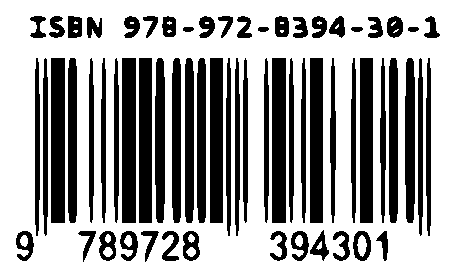
\includegraphics[width=35mm]{ISBN-code-3.eps}
% \hskip 10mm\raise 17mm\hbox{\vtop{\hsize 90mm\noindent
% Universidade de Lisboa
% \hfil\break Faculdade de Ci\^encias
% \hfil\break Departamento de Matem\'atica
% \hfil\break %\phantom{$\displaystyle\int$}
% \hfil\break first edition, February 2021}}

% \vfil
\vskip 100mm

\noindent
Copyright 2020, 2021, 2022 Cristian Barbarosie {\small\tt cristian.barbarosie@gmail.com}
\bigskip

\noindent
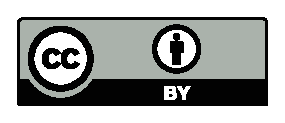
\includegraphics[width=35mm]{common-creatives-by.eps}\hskip5mm
\raise 9mm\hbox{\vtop{\hsize 110mm\noindent
This manual is licensed under the
\hfil\break Creative Commons Attribution 4.0 International License :
\hfil\break{\tt https://creativecommons.org/licenses/by/4.0/}}}

%%%%%%%%%%%%%%%%%%%%%%%%%%%%%%%%%%%%%%%%%%%%%%%%%%%%%%%%%%%%%%%%%%%%%%%%%%%%%%%%%%%%%%%%%%%%%%%

\tableofcontents

%%%%%%%%%%%%%%%%%%%%%%%%%%%%%%%%%%%%%%%%%%%%%%%%%%%%%%%%%%%%%%%%%%%%%%%%%%%%%%%%%%%%%%%%%%%%%%%



          %-------------------%
\chapter{~~General description}\label{\numb section 1}
          %-------------------%

This section is a quick tour through \maniFEM's capabilities.
There is also a gallery with several examples at
{\small\tt http://manifem.rd.ciencias.ulisboa.pt/gallery/}


          %---------------------%
\section{~~An elementary example}\label{\numb section 1.\numb parag 1}
          %---------------------%

In this paragraph, we show how to build a rectangular mesh on a surface in $ \mathbb{R}^3 $ 
and then compute the integral of a given function.
Paragraph \ref{\numb section 1.\numb parag 4} shows a purely two-dimensional example.

\begin{figure} \centering
  \psfrag{SW}{\small\tt\textcolor{textindraw}{SW}}
  \psfrag{NW}{\small\tt\textcolor{textindraw}{NW}}
  \psfrag{SE}{\small\tt\textcolor{textindraw}{SE}}
  \psfrag{NE}{\small\tt\textcolor{textindraw}{NE}}
  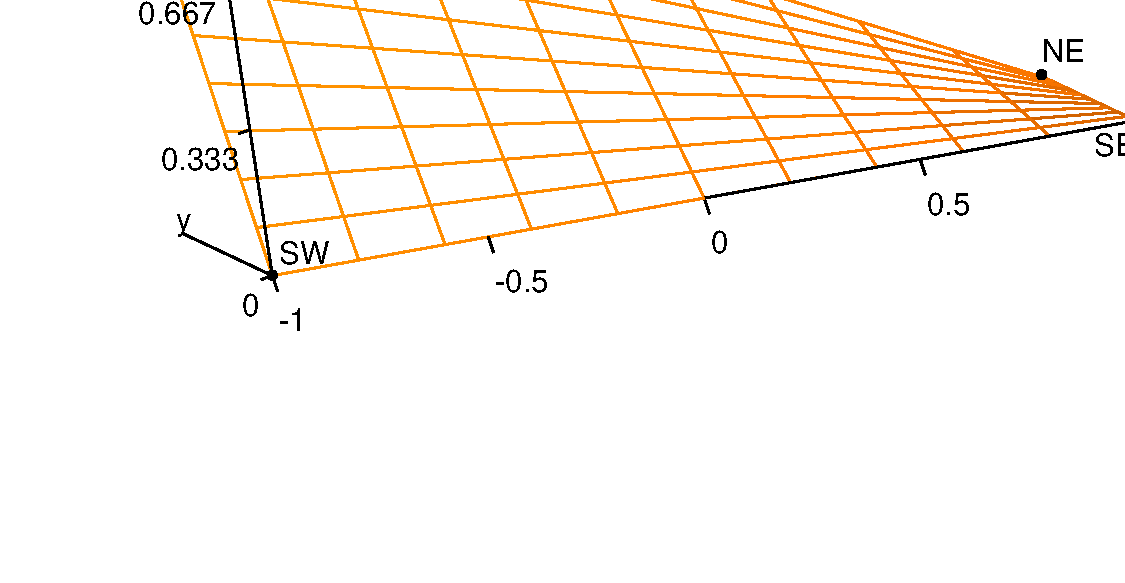
\includegraphics[width=105mm]{3d-rectangle}
  \caption{A twisted rectangular mesh}
  \label{\numb section 1.\numb fig 1}
\end{figure}

\begin{Verbatim}[commandchars=\\\{\},formatcom=\small\tt,frame=single,
   label=parag-\ref{\numb section 1.\numb parag 1}.cpp,rulecolor=\color{moldura},
   baselinestretch=0.94,framesep=2mm                                            ]
#include \verde{"maniFEM.h"}

using namespace \verm{maniFEM};
using namespace std;

int main ()

\{  \cinza{// we choose our (geometric) space dimension :}
   \verm{Manifold} \azul{RR3} ( \textcolor{tag}{tag}::Euclid, \textcolor{tag}{tag}::of_dim, \laranja{3} );
   
   \cinza{// xyz is a map defined on our future mesh with values in RR3 :}
   \verm{Function} \azul{xyz} = RR3 .build_coordinate_system ( \textcolor{tag}{tag}::Lagrange, \textcolor{tag}{tag}::of_degree, \laranja{1} );

   \cinza{// we can extract components of xyz using the [] operator}
   \verm{Function} \azul{x} = xyz[\laranja{0}], \azul{y} = xyz[\laranja{1}], \azul{z} = xyz[\laranja{2}];

   \cinza{// Let's build a rectangular mesh. First, the four corners :}
   \verm{Cell} \azul{SW} ( \textcolor{tag}{tag}::vertex );  x(SW) = \laranja{-1.};  y(SW) = \laranja{0.};  z(SW) = \laranja{0.};
   \verm{Cell} \azul{SE} ( \textcolor{tag}{tag}::vertex );  x(SE) =  \laranja{1.};  y(SE) = \laranja{0.};  z(SE) = \laranja{0.};
   \verm{Cell} \azul{NE} ( \textcolor{tag}{tag}::vertex );  x(NE) =  \laranja{1.};  y(NE) = \laranja{1.};  z(NE) = \laranja{0.};
   \verm{Cell} \azul{NW} ( \textcolor{tag}{tag}::vertex );  x(NW) = \laranja{-1.};  y(NW) = \laranja{1.};  z(NW) = \laranja{1.};
   \cinza{// alternative syntax for declaring vertices :}
   \cinza{// Cell SW ( tag::vertex, tag::of_coords, \{ -1., 0., 0. \} )}
   \cinza{// Cell SE ( tag::vertex, tag::of_coords, \{  1., 0., 0. \} )}
   \cinza{// Cell NE ( tag::vertex, tag::of_coords, \{  1., 1., 0. \} )}
   \cinza{// Cell NW ( tag::vertex, tag::of_coords, \{ -1., 1., 1. \} )}
   
   \cinza{// we access the coordinates of a point using the () operator :}
   cout << \verde{"coordinates of NW : "} << x(NW) << \verde{" "} << y(NW) << \verde{" "} << z(NW) << endl;

   \cinza{// now build the four sides of the rectangle :}
   \verm{Mesh} \azul{south} ( \textcolor{tag}{tag}::segment, SW .reverse(), SE, \textcolor{tag}{tag}::divided_in, \laranja{10} );
   \verm{Mesh} \azul{east}  ( \textcolor{tag}{tag}::segment, SE .reverse(), NE, \textcolor{tag}{tag}::divided_in, \laranja{10} );
   \verm{Mesh} \azul{north} ( \textcolor{tag}{tag}::segment, NE .reverse(), NW, \textcolor{tag}{tag}::divided_in, \laranja{10} );
   \verm{Mesh} \azul{west}  ( \textcolor{tag}{tag}::segment, NW .reverse(), SW, \textcolor{tag}{tag}::divided_in, \laranja{10} );
   
   \cinza{// and now the rectangle :}
   \verm{Mesh} \azul{rect_mesh} ( \textcolor{tag}{tag}::rectangle, south, east, north, west );

   \cinza{// we may want to visualize the resulting mesh}
   \cinza{// here is one way to export the mesh in the "msh" format :}
   rect_mesh .export_to_file ( \textcolor{tag}{tag}::msh, \verde{"rectangle.msh"});

   \cinza{// let's define a symbolic function}
   \verm{Function} \azul{f} = x*x + \laranja{1}/(\laranja{5}+y);

   \cinza{// and compute its integral on the rectangle,}
   \cinza{// using, in each rectangular cell, Gauss quadrature with 9 points :}
   \verm{Integrator} \azul{integr} ( \textcolor{tag}{tag}::Gauss, \textcolor{tag}{tag}::quad_9 );

   cout << \verde{"integral of f "} << integr ( f, \textcolor{tag}{tag}::on, rect_mesh ) << endl;

\}  \cinza{// end of main}
\end{Verbatim}

Paragraph \ref{\numb section 11.\numb parag 2} explains the coloring conventions observed
in this manual for {\tt C++} code.

To run this example, you will need a recent {\tt C++} compiler and the {\tt make} utility.
Visit {\small\tt https://github.com/cristian-barbarosie/manifem}, choose a release
and download all files to some directory in your computer.
Paragraph \ref{\numb section 11.\numb parag 16} gives more details.
% Latest code may be unstable, releases are stable.
Launch the program through the command
{\small\tt make run-\ref{\numb section 1.\numb parag 1}};
a file {\small\tt rectangle.msh} should appear in the working directory.
You may view the mesh using the software {\tt gmsh}.

Expressions like {\small\tt\textcolor{tag}{tag}::of\_\,dim} and
{\small\tt\textcolor{tag}{tag}::vertex} are
objects belonging to the {\small\tt namespace} {\small\tt\verm{tag}};
we use them as arguments to many functions.
See paragraph \ref{\numb section 11.\numb parag 3} for some details.

Paragraph \ref{\numb section 5.\numb parag 1} explains why we build {\small\tt\verm{Function}}
{\small\tt\azul{xyz}} with arguments {\small\tt\textcolor{tag}{tag}::Lagrange,}\hfil\break
{\small\tt\textcolor{tag}{tag}::of\_\,degree,} {\small\tt\laranja{1}}.

When declaring a segment {\small\tt\verm{Mesh}}, we must {\small\tt reverse} the first vertex
(paragraph \ref{\numb section 1.\numb parag 2} discusses the {\small\tt reverse} method).
Paragraph \ref{\numb section 1.\numb parag 4} explains why we build
the rectangle based on its four sides rather than on its four vertices.

Note that in this example we do not have exact control on the shape of the surface being meshed.
The coordinates of the inner vertices are defined rather vaguely by interpolating the
coordinates of the four corners.
See sections \ref{\numb section 2} and \ref{\numb section 3} for ways to precisely define
a submanifold in $ \mathbb{R}^3 $ and mesh (a bounded domain of) it.


          %----------------%
\section{~~Cells and meshes}\label{\numb section 1.\numb parag 2}
          %----------------%

In \maniFEM, all basic constituents of meshes are called ``cells''. 
Points are zero-dimensional cells, segments are one-dimensional cells, triangles are
two-dimensional cells, and so on.

Roughly speaking, a mesh is a collection of cells of the same dimension. 
For efficiency reasons, meshes keep lists of cells of lower dimension, too. 
For instance, the mesh built in paragraph \ref{\numb section 1.\numb parag 1} is 
roughly a list of two-dimensional cells (quadrilaterals), but lists of segments and points
are also kept.
This represents quite some amount of redundant information, but it is useful e.g.\ for
quickly sweeping over all vertices of a mesh.%
\footnote {{} Actually, the implementation details are more complicated.
There are different kinds of meshes, some of them keep more information (lists of cells)
and are faster; others are slower but lighter in terms of memory occupied.
See e.g. paragraph \ref{\numb section 11.\numb parag 6}.}

A cell of dimension $ d>0 $ is defined by its boundary, 
which in turn is a mesh of dimension $ d-1 $. 
The boundary of a segment is a (zero-dimensional) mesh made of two points.
The boundary of a triangle is a one-dimensional mesh made of three segments.
Thus, a segment is essentially a pair of points, a triangle is essentially a triplet of segments, and so on.

Cells and meshes are oriented. 
An orientation of a mesh is just an orientation for each of its component cells
(of course these orientations must be mutually compatible).
Although this is not how the orientation is implemented internally
(see paragraph \ref{\numb section 11.\numb parag 4}),
an oriented point can be conceived simply as a point with a sign attached (1 or -1). 
The orientation of a cell of dimension higher than zero is given by an orientation
of its boundary, which is a lower-dimensional mesh.

Thus, an oriented segment is essentially a pair of points, one of which has a \hbox{-1}
attached, the other having a 1.
We call the former ``base'' and the latter ``tip''.
These signs are related to integration of functions along that segment.
The integral of a function of one variable is equal to the value of the 
primitive function at one end of the segment minus the value of the primitive at the other end.

An oriented triangle is essentially a triplet of segments, each one with its own orientation.
The orientations must be compatible to each other in the sense that each vertex 
must be seen as positive by one of the segments and as negative by another one.
An oriented tetrahedron can be identified with four triangles, each one with its own
orientation.
In such a tetrahedron, each segment must be seen as positive by one of the triangles and
as negative by another one.

\begin{figure}[ht] \centering
  \psfrag{A}{\small\tt\textcolor{textindraw}{A}}
  \psfrag{B}{\small\tt\textcolor{textindraw}{B}}
  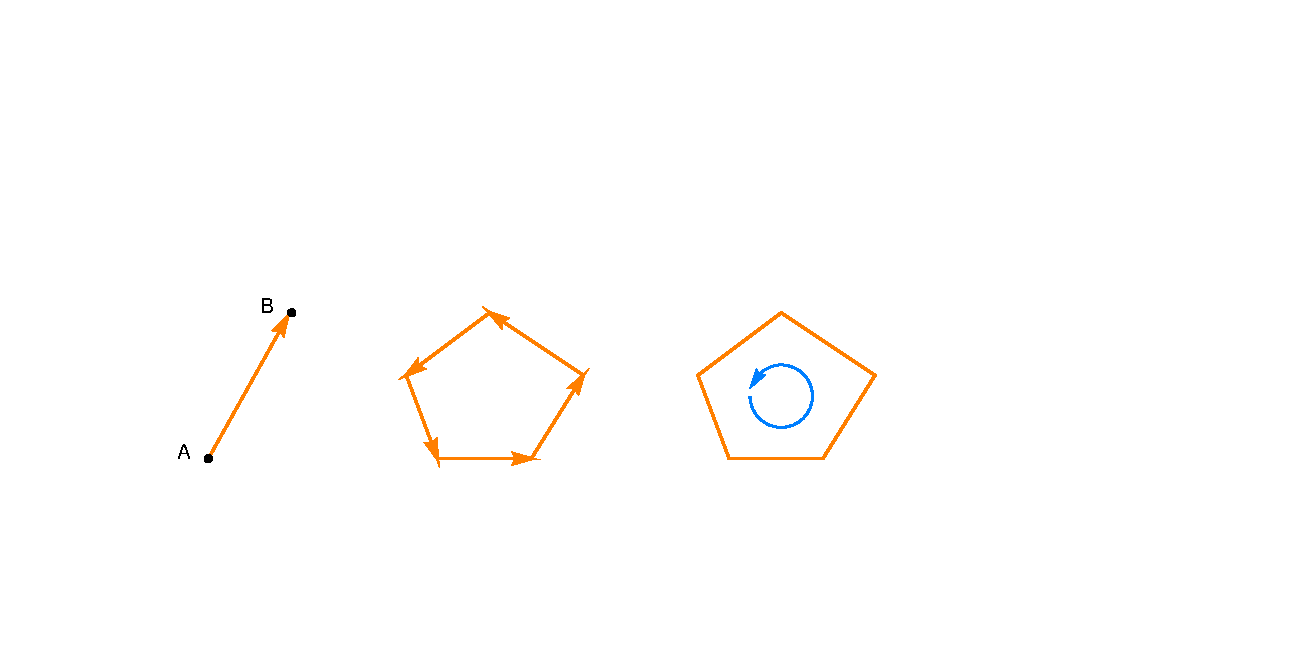
\includegraphics[width=90mm]{oriented-cells.eps}
  \caption{Oriented segment, oriented pentagon}
  \label{\numb section 1.\numb fig 2}
\end{figure}

We can think of an oriented segment as an arrow pointing from its negative extremity (base)
towards its positive extremity (tip).
We can think of an oriented polygon as having an arrow attached to each of it sides,
or we can imagine a small oriented circle inside the polygon.

\begin{figure} \centering
  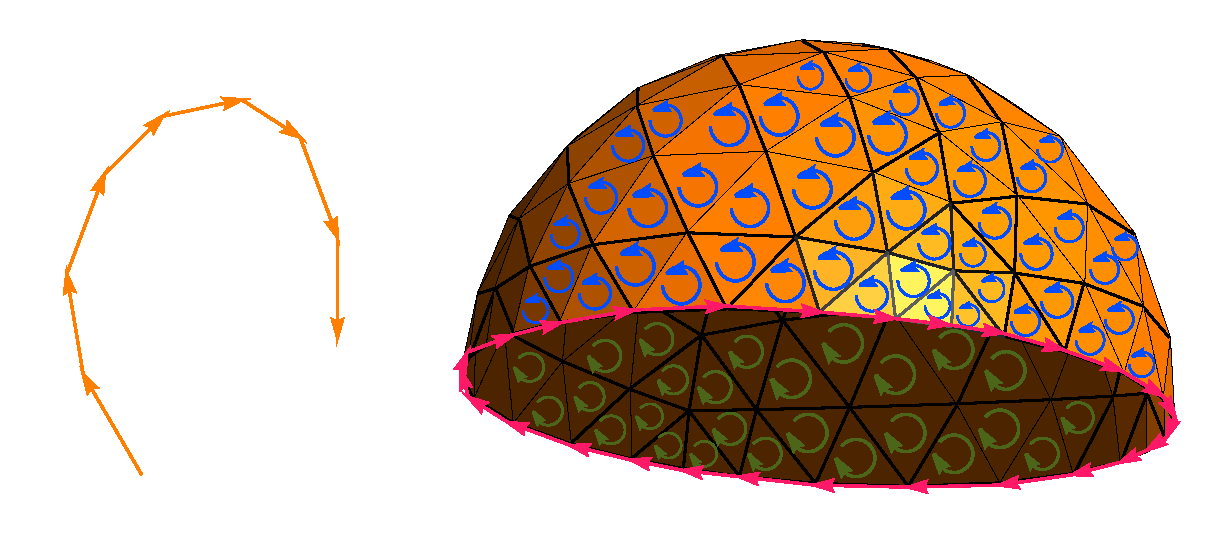
\includegraphics[width=115mm]{hemisphere-7}
  \caption{Oriented meshes of dimension one and two}
  \label{\numb section 1.\numb fig 3}
\end{figure}

A one-dimensional oriented mesh can be thought of as a chain of arrows,
each one pointing to the next segment's base (like in figure \ref{\numb section 1.\numb fig 3}
right).
A two-dimensional oriented triangular mesh can be thought of as a web of triangles,
each triangle having a small oriented circle inside (like in figure
\ref{\numb section 1.\numb fig 3} left).
The orientations of neighbour cells must be compatible : each segment must be seen
in opposite orientations from the point of view of its two neighbour triangles.

The above description of the orientation of a two-dimensional mesh does not depend
on the surrounding space.
A mesh can be immersed in some Euclidian space $ \mathbb{R}^d $ or not.
As an extreme example, vertices may even have no coordinates at all.
However, in the case of a two-dimensional mesh immersed in $ \mathbb{R}^3 $,
the right hand rule establishes a correspondence between the oriented circle described above
and an arrow normal to the surface being meshed.
Note that the right hand rule is a convention based on the assuption that
the surrounding space $ \mathbb{R}^3 $ has a certain orientation.

Note also that an orientation of a mesh defines an orientation of its boundary.
In figure \ref{\numb section 1.\numb fig 3} we can see the orientation of the
boundary of the mesh, shown with pink arrows.
This convention is used by Stokes' theorem.

Figure \ref{\numb section 1.\numb fig 4} shows two opposite orientations of a mesh,
together with the corresponding orientation of its boundary.

\begin{figure}[ht] \centering
\begin{subfigure}{75mm}\centering
  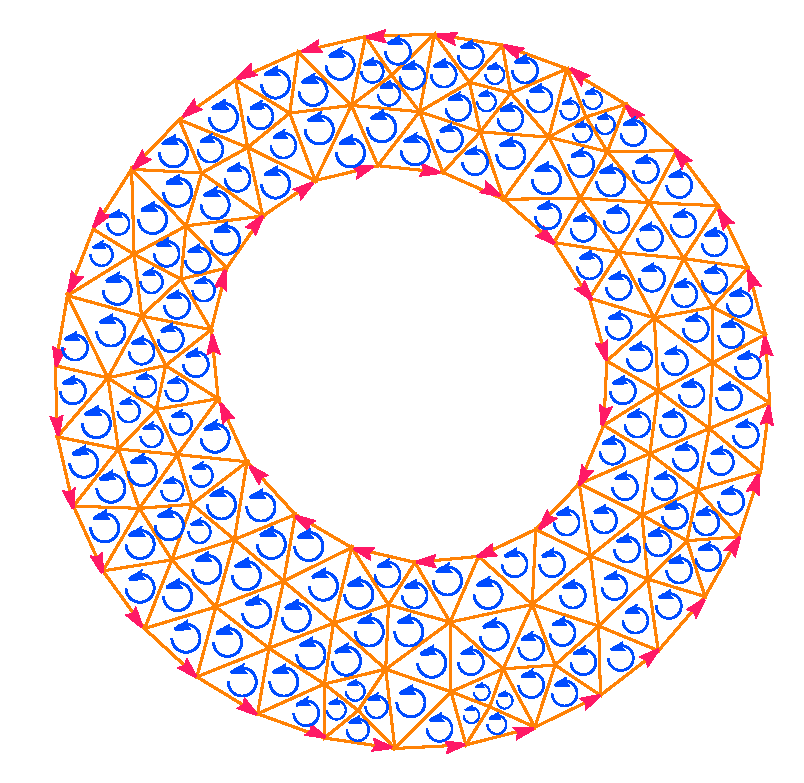
\includegraphics[width=74mm]{oriented-annulus-1}
\end{subfigure}  
\begin{subfigure}{75mm}\centering
  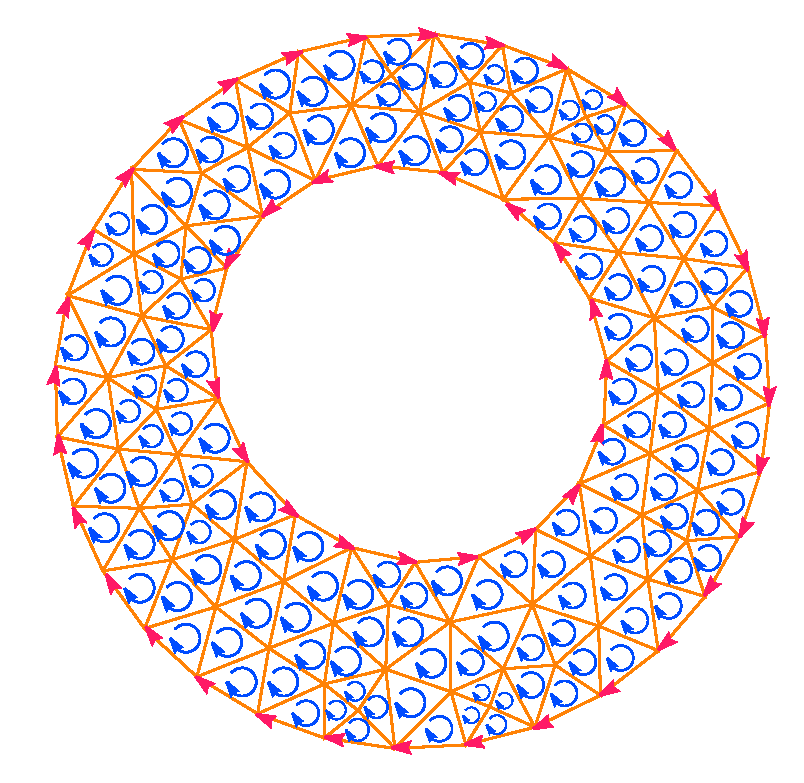
\includegraphics[width=74mm]{oriented-annulus-2}
\end{subfigure}  
  \caption{Mesh with two opposite orientations}
  \label{\numb section 1.\numb fig 4}
\end{figure}

Often, when building a {\small\tt\verm{Mesh}}, {\maniFEM} chooses the orientation based
on the orientation of the boundary, as provided by the user.
For instance, in a statement like

\begin{Verbatim}[commandchars=\\\{\},formatcom=\small\tt,baselinestretch=0.94]
   \verm{Mesh} \azul{rect_mesh} ( \textcolor{tag}{tag}::rectangle, south, east, north, west );
\end{Verbatim}

\noindent (used in paragraphs \ref{\numb section 1.\numb parag 1},
\ref{\numb section 1.\numb parag 4} and many others)
the orientation of {\small\tt\azul{rect\_\,mesh}} is defined by the orientation of
its four sides (which must be mutually compatible).
If we switch all four orientations, we will obtain the same mesh with the opposite orientation.
This can be done either by changing the declaration of each side (switching the first vertex with
the last) or by replacing (in the above declaration of {\small\tt\azul{rect\_\,mesh}})
{\small\tt south} by {\small\tt south} {\small\tt .reverse()},
{\small\tt east} by {\small\tt east.} {\small\tt .reverse()} and so on.
The {\small\tt reverse} method is explained below.
If we switch the orientation of one side only, {\maniFEM} will complain that
the orientations are not compatible with each other.

In paragraphs \ref{\numb section 1.\numb parag 4} and \ref{\numb section 3.\numb parag 19},
special attention is given to the orientation of the common boundary of meshes to be
subsequently joined.
In frontal mesh generation (described in section \ref{\numb section 3}) we often
provide the boundary of the future mesh, whose orientation determines the output of the
algorithm.

{\ManiFEM} distinguishes between cells (which are geometric entities) and finite elements.
We may have different finite elements whose geometry is the same.
For instance, we may have triangular Lagrange finite elemens of different degrees;
they will all dock on the same triangular cell.
Paragraph \ref{\numb section 6.\numb parag 1} gives more details.

Cells have a {\small\tt reverse} method returning the reversed cell.
Segment {\small\tt\verm{Cell}}s have methods {\small\tt base} and {\small\tt tip}
returning their extremities.
For instance :

\begin{Verbatim}[commandchars=\\\{\},formatcom=\small\tt,baselinestretch=0.94]
   \verm{Cell} \azul{A} ( \textcolor{tag}{tag}::vertex );  \verm{Cell} \azul{B} ( \textcolor{tag}{tag}::vertex );
   assert ( A .is_positive() );
   assert ( not A .reverse() .is_positive() );
   assert ( A .reverse() .reverse() == A );
   \verm{Cell} \azul{AB} ( \textcolor{tag}{tag}::segment, A .reverse(), B );  \cinza{// here, AB is a segment Cell, not a Mesh}
   assert ( AB .base() == A .reverse() );
   assert ( AB .tip() == B );

   \verm{Cell} \azul{BA} = AB .reverse();
   assert ( BA .base() == B .reverse() );
   assert ( BA .tip() == A );
   assert ( BA .reverse() == AB );
\end{Verbatim}

Paragraph \ref{\numb section 9.\numb parag 5} gives more details about the orientation of cells.
See also paragraph \ref{\numb section 11.\numb parag 4}.

Cells are topological entities; they carry no geometric information.
In particular, points do not have coordinates.
Coordinates are stored (semi-)externally, see paragraphs \ref{\numb section 5.\numb parag 1} and
\ref{\numb section 13.\numb parag 6}.

{\small\tt \verm{Mesh}}es have a {\small\tt reverse} method, too.
It is used mainly when we want to {\small\tt join} meshes having a common piece of boundary;
see paragraphs \ref{\numb section 1.\numb parag 4}, \ref{\numb section 2.\numb parag 6},
\ref{\numb section 2.\numb parag 7}, \ref{\numb section 2.\numb parag 14},
\ref{\numb section 3.\numb parag 17}, \ref{\numb section 3.\numb parag 19}.

Below we show a low-level way of building a tiny mesh, made of two triangles only.
We stress that there are shorter and more elegant mesh constructors, see paragraphs
\ref{\numb section 1.\numb parag 1}, \ref{\numb section 1.\numb parag 4} --
\ref{\numb section 1.\numb parag 6}, sections \ref{\numb section 2} and \ref{\numb section 3}.

\begin{Verbatim}[commandchars=\\\{\},formatcom=\small\tt,baselinestretch=0.94]
   \verm{Cell} \azul{C} ( \textcolor{tag}{tag}::vertex );
   \verm{Cell} \azul{BC} ( \textcolor{tag}{tag}::segment, B .reverse(), C );
   \verm{Cell} \azul{CA} ( \textcolor{tag}{tag}::segment, C .reverse(), A );
   \verm{Cell} \azul{ABC} ( \textcolor{tag}{tag}::triangle, AB, BC, CA );
   \verm{Cell} \azul{D} ( \textcolor{tag}{tag}::vertex );
   \verm{Cell} \azul{AD} ( \textcolor{tag}{tag}::segment, A .reverse(), D );
   \verm{Cell} \azul{DB} ( \textcolor{tag}{tag}::segment, D .reverse(), B );
   \verm{Cell} \azul{BAD} ( \textcolor{tag}{tag}::triangle, AB .reverse(), AD, DB );
   \verm{Mesh} \azul{msh} ( \textcolor{tag}{tag}::fuzzy, \textcolor{tag}{tag}::of_dim, \laranja{2} );
   ABC .add_to_mesh ( msh );
   BAD .add_to_mesh ( msh );
\end{Verbatim}


          %---------%
\section{~~Functions}\label{\numb section 1.\numb parag 3}
          %---------%

Minimalist programs like the pieces of code presented in paragraph
\ref{\numb section 1.\numb parag 2} (consisting mainly of manipulation of
{\small\tt\verm{Cell}}s) work without declaring a {\small\tt\verm{Manifold}}
and without {\small\tt\verm{Function}}s.
However, most {\small\tt\verm{Mesh}} constructors will try to interpolate geometric coordinates
based on the shape of the current {\small\tt\verm{Manifold}}.

{\small\tt\verm{Function}}s in {\maniFEM} can be divided roughly in two categories.
Some keep numeric values, like {\small\tt x}, {\small\tt y} and {\small\tt z}
encountered in many places in this manual.
After building a function like

\begin{Verbatim}[commandchars=\\\{\},formatcom=\small\tt,baselinestretch=0.94]
   \verm{Function} \azul{xyz} = RR3 .build_coordinate_system ( \textcolor{tag}{tag}::Lagrange, \textcolor{tag}{tag}::of_degree, \laranja{1} );
\end{Verbatim}

\noindent the process of creating a new vertex will change.
Space in the computer's memory will be reserved for {\small\tt d} values of type
{\small\tt double} ({\small\tt d} being the dimension of the {\small\tt\verm{Manifold}},
here {\small\tt RR3}) for each new vertex.
The components of {\small\tt xyz} can be extracted like in

\begin{Verbatim}[commandchars=\\\{\},formatcom=\small\tt,baselinestretch=0.94]
   \verm{Function} \azul{x} = xyz[\laranja{0}], \azul{y} = xyz[\laranja{1}], \azul{z} = xyz[\laranja{2}];
\end{Verbatim}

\noindent They are mere handlers through which we access the above referred \ {\small\tt double}
\ values, like in {\small\tt x(A)} {\small\tt =} {\small\tt \laranja{1.}}\ or
{\small\tt double} {\small\tt \azul{sum}} {\small\tt =} {\small\tt x(A)} {\small\tt +}
{\small\tt y(B)} {\small\tt +} {\small\tt z(C)}.
Actually, the interaction between the {\small\tt\verm{Function}} object and the values
associated to each vertex involves other layers, one of which is a {\small\tt\verm{Field}}
object.
In most cases, these layers are invisible to the final user.

Other {\small\tt\verm{Function}}s are not related with space in the computer's memory
(they have no subjacent {\small\tt\verm{Field}}).
For instance, there are arithmetic expressions like 

\begin{Verbatim}[commandchars=\\\{\},formatcom=\small\tt,baselinestretch=0.94]
   \verm{Function} \azul{norm} = \verm{power} ( x*x + y*y + z*z, \laranja{0.5} );
\end{Verbatim}

We can still access the value of such a {\small\tt\verm{Function}} at a cell like in
{\small\tt double} {\small\tt \azul{n}} {\small\tt =} {\small\tt norm(A)};
the computer will return the value of the corresponding arithmetic expression,
replacing the symbols {\small\tt x}, {\small\tt y} and {\small\tt z} by the corresponding
values at cell {\small\tt A}.
But it makes no sense to change the value of {\small\tt norm} at cell {\small\tt A}.
Thus, statements like {\small\tt x(A)} {\small\tt =} {\small\tt\laranja{1.}} work fine,
while {\small\tt norm(A)} {\small\tt =} {\small\tt\laranja{1.}} produces a run-time error.

The {\small\tt\verm{Function}::deriv} method performs symbolic differentiation :

\begin{Verbatim}[commandchars=\\\{\},formatcom=\small\tt,baselinestretch=0.94]
   \verm{Function} \azul{norm_x} = norm .deriv (x);
   \verm{Function} \azul{norm_y} = norm .deriv (y);
\end{Verbatim}

Integrals of {\small\tt\verm{Function}}s are computed by means of {\small\tt\verm{Integrator}}s,
either alone or coupled with a {\small\tt\verm{FiniteElement}}.
Section \ref{\numb section 6} gives more details.


          %--------------%
\section{~~Joining meshes}\label{\numb section 1.\numb parag 4}
          %--------------%

The example in paragraph \ref{\numb section 1.\numb parag 1} could have been shortened
had we used the overloaded version of the {\small\tt \verm{Mesh}} constructor with
{\small\tt \textcolor{tag}{tag}::rectangle} which accepts the four corners as arguments. 
This overloaded version exists in \maniFEM, but we prefer to build meshes in a structured way, 
first corners, then sides and then the plane region. 
This has the advantage that one can build more complex meshes from simple components. 
For instance, one can build an L-shaped mesh by joining three rectangular meshes :

\begin{Verbatim}[commandchars=\\\{\},formatcom=\small\tt,frame=single,
   label=parag-\ref{\numb section 1.\numb parag 4}.cpp,rulecolor=\color{moldura},
   baselinestretch=0.94,framesep=2mm]
   \verm{Manifold} \azul{RR2} ( \textcolor{tag}{tag}::Euclid, \textcolor{tag}{tag}::of_dim, \laranja{2} );
   \verm{Function} \azul{xy} = RR2 .build_coordinate_system ( \textcolor{tag}{tag}::Lagrange, \textcolor{tag}{tag}::of_degree, \laranja{1} );
   \verm{Function} \azul{x} = xy[\laranja{0}], \azul{y} = xy[\laranja{1}];
   \verm{Cell} \azul{A} ( \textcolor{tag}{tag}::vertex, \textcolor{tag}{tag}::of_coords, \{ \laranja{-1.}, \laranja{0.}  \} );
   \verm{Cell} \azul{A} ( \textcolor{tag}{tag}::vertex, \textcolor{tag}{tag}::of_coords, \{ \laranja{-1.}, \laranja{0.}  \} );
   \verm{Cell} \azul{B} ( \textcolor{tag}{tag}::vertex, \textcolor{tag}{tag}::of_coords, \{  \laranja{0.}, \laranja{0.}  \} );
   \verm{Cell} \azul{C} ( \textcolor{tag}{tag}::vertex, \textcolor{tag}{tag}::of_coords, \{  \laranja{0.}, \laranja{0.5} \} );
   \verm{Cell} \azul{D} ( \textcolor{tag}{tag}::vertex, \textcolor{tag}{tag}::of_coords, \{ \laranja{-1.}, \laranja{0.5} \} );
   \verm{Cell} \azul{E} ( \textcolor{tag}{tag}::vertex, \textcolor{tag}{tag}::of_coords, \{  \laranja{0.}, \laranja{1.}  \} );
   \verm{Cell} \azul{F} ( \textcolor{tag}{tag}::vertex, \textcolor{tag}{tag}::of_coords, \{ \laranja{-1.}, \laranja{1.}  \} );
   \verm{Cell} \azul{G} ( \textcolor{tag}{tag}::vertex, \textcolor{tag}{tag}::of_coords, \{  \laranja{1.}, \laranja{0.}  \} );
   \verm{Cell} \azul{H} ( \textcolor{tag}{tag}::vertex, \textcolor{tag}{tag}::of_coords, \{  \laranja{1.}, \laranja{0.5} \} );

   \verm{Mesh} \azul{AB} ( \textcolor{tag}{tag}::segment, A .reverse(), B, \textcolor{tag}{tag}::divided_in, \laranja{10} );
   \verm{Mesh} \azul{BC} ( \textcolor{tag}{tag}::segment, B .reverse(), C, \textcolor{tag}{tag}::divided_in,  \laranja{8} );
   \verm{Mesh} \azul{CD} ( \textcolor{tag}{tag}::segment, C .reverse(), D, \textcolor{tag}{tag}::divided_in, \laranja{10} );
   \verm{Mesh} \azul{DA} ( \textcolor{tag}{tag}::segment, D .reverse(), A, \textcolor{tag}{tag}::divided_in,  \laranja{8} );
   \verm{Mesh} \azul{CE} ( \textcolor{tag}{tag}::segment, C .reverse(), E, \textcolor{tag}{tag}::divided_in,  \laranja{7} );
   \verm{Mesh} \azul{EF} ( \textcolor{tag}{tag}::segment, E .reverse(), F, \textcolor{tag}{tag}::divided_in, \laranja{10} );
   \verm{Mesh} \azul{FD} ( \textcolor{tag}{tag}::segment, F .reverse(), D, \textcolor{tag}{tag}::divided_in,  \laranja{7} );
   \verm{Mesh} \azul{BG} ( \textcolor{tag}{tag}::segment, B .reverse(), G, \textcolor{tag}{tag}::divided_in, \laranja{12} );
   \verm{Mesh} \azul{GH} ( \textcolor{tag}{tag}::segment, G .reverse(), H, \textcolor{tag}{tag}::divided_in,  \laranja{8} );
   \verm{Mesh} \azul{HC} ( \textcolor{tag}{tag}::segment, H .reverse(), C, \textcolor{tag}{tag}::divided_in, \laranja{12} );

   \verm{Mesh} \azul{ABCD} ( \textcolor{tag}{tag}::rectangle, AB, BC, CD, DA );
   \verm{Mesh} \azul{CEFD} ( \textcolor{tag}{tag}::rectangle, CE, EF, FD, CD .reverse() );
   \verm{Mesh} \azul{BGHC} ( \textcolor{tag}{tag}::rectangle, BG, GH, HC, BC .reverse() );

   \verm{Mesh} \azul{L_shaped} ( \textcolor{tag}{tag}::join, ABCD, CEFD, BGHC );
\end{Verbatim}

\begin{figure}[ht] \centering
  \psfrag{A}{\small\tt\textcolor{textindraw}{A}}
  \psfrag{B}{\small\tt\textcolor{textindraw}{B}}
  \psfrag{C}{\small\tt\textcolor{textindraw}{C}}
  \psfrag{D}{\small\tt\textcolor{textindraw}{D}}
  \psfrag{E}{\small\tt\textcolor{textindraw}{E}}
  \psfrag{F}{\small\tt\textcolor{textindraw}{F}}
  \psfrag{G}{\small\tt\textcolor{textindraw}{G}}
  \psfrag{H}{\small\tt\textcolor{textindraw}{H}}
  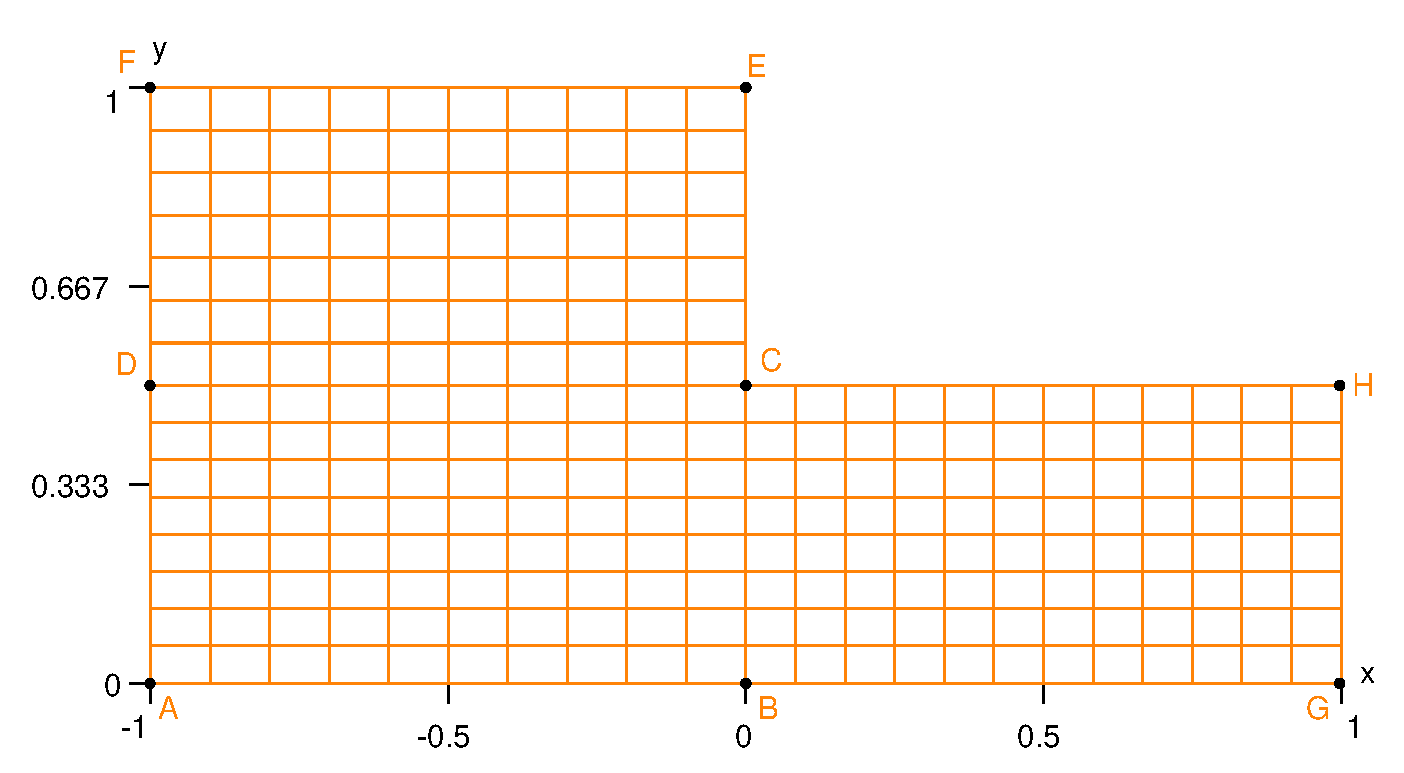
\includegraphics[width=115mm]{L-shaped}
  \caption{An L-shaped mesh}
  \label{\numb section 1.\numb fig 5}
\end{figure}

Meshes in $ \mathbb{R}^2 $ like the one above may be exported in the {\small\tt msh} format
or directly drawn in {\small\tt PostScript}, by one of the two statements below

\begin{Verbatim}[commandchars=\\\{\},formatcom=\small\tt,baselinestretch=0.94]
   L_shaped .export_to_file ( \textcolor{tag}{tag}::msh, \verde{"L-shaped.msh"});
   L_shaped .draw_ps (\verde{"L-shaped.eps"});
\end{Verbatim}

Note that, in \maniFEM, cells and meshes are oriented
(see paragraph \ref{\numb section 1.\numb parag 2}).
To build {\small\tt \azul{CEFD}} one must use not {\small\tt CD} but its reverse;
to build {\small\tt \azul{BGHC}} one must use not {\small\tt BC} but its reverse.
In figure \ref{\numb section 1.\numb fig 6} we see a zoom around {\small\tt C};
the three rectangular meshes have been separated just for visualization purposes.
The drawing illustrates that the common boundary has a certain orientation when seen
from one mesh and has the opposite orientation when seen from the neighbour mesh.
If we do not respect these orientations, {\maniFEM} will be unable to {\small\tt join}
these meshes.

\begin{figure}[ht]  \centering
  \psfrag{C}{\small\tt\textcolor{textindraw}{C}}
  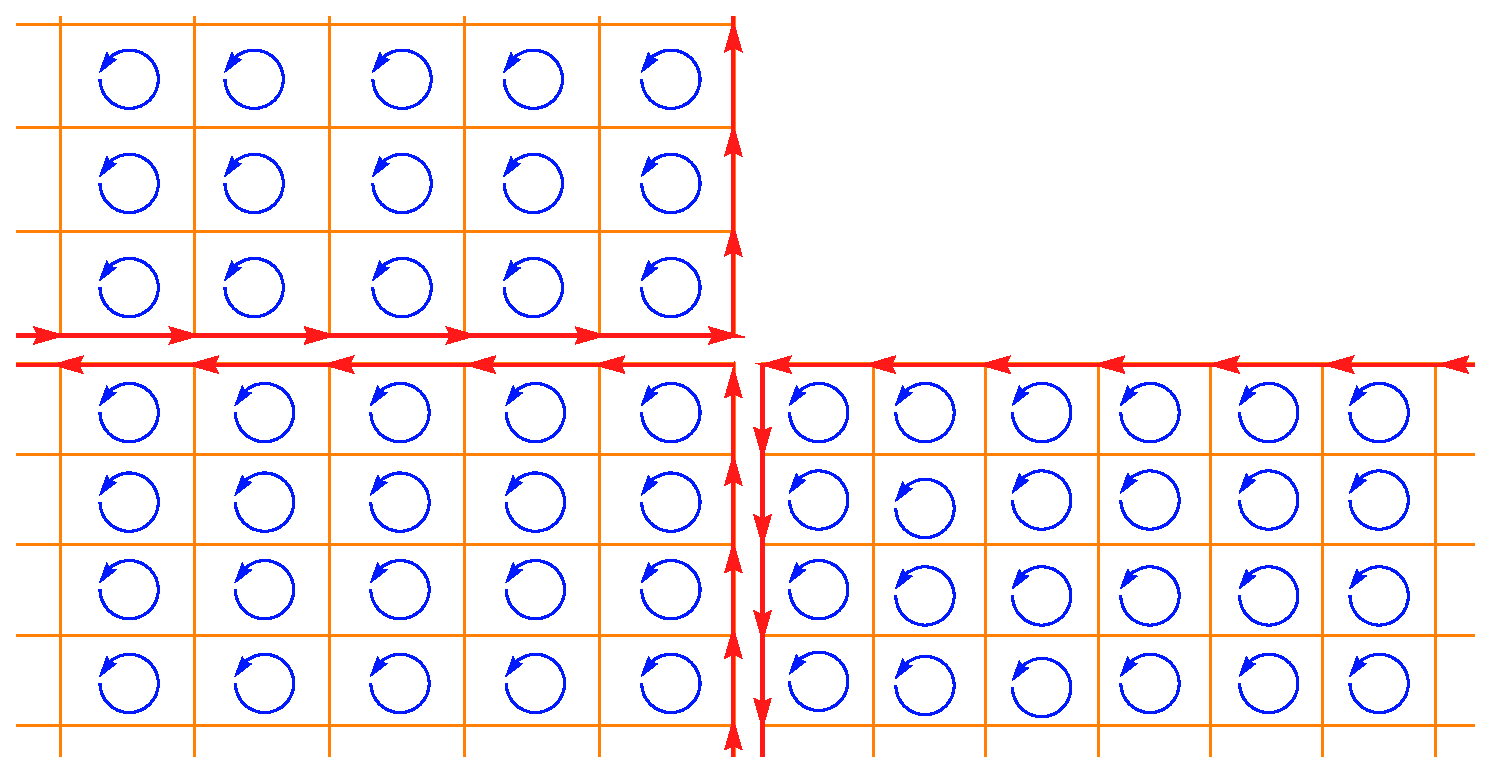
\includegraphics[width=120mm]{L-crack}
  \caption{A zoom around {\small\tt C}}
  \label{\numb section 1.\numb fig 6}
\end{figure}

We can imagine a magnet attached to each face of a cell.
For two neighbour cells, the common face will have two magnets, one from each cell.
If their polarities are not opposite, the magnets will not cling.
Likewise, the common boundary of two meshes that we intend to join can be thought of
as a pair of magnets.
If their polarities are not opposite, the two meshes will not cling.

Note also that if we define the rectangles based on their vertices instead of their sides, 
the {\small\tt\verm{Mesh}} constructor with {\small\tt \textcolor{tag}{tag}::join} will
not work properly. 
For instance, the two rectangles defined by

\begin{Verbatim}[commandchars=\\\{\},formatcom=\small\tt,baselinestretch=0.94]
   \verm{Mesh} \azul{ABCD} ( \textcolor{tag}{tag}::rectangle, A, B, C, D, \textcolor{tag}{tag}::divided_in, \laranja{10}, \laranja{8} );
   \verm{Mesh} \azul{CEFD} ( \textcolor{tag}{tag}::rectangle, C, E, F, D, \textcolor{tag}{tag}::divided_in, \laranja{7}, \laranja{10} );
\end{Verbatim}

\noindent cannot be joined$\,$%
\footnote {{} Actually, they can be joined but the resulting mesh will have
a crack along {\small\tt CD} -- probably not what the user wants.}
because the side {\small\tt CD} of {\small\tt ABCD} has nothing to do with the side 
{\small\tt DC} of {\small\tt CEFD}.
These two sides are one-dimensional meshes both made of 10 segments but with different
interior points (only {\small\tt C} and {\small\tt D} are shared) and different segments.
In contrast, {\small\tt CD} and {\small\tt CD.reverse()} share the same 11 points and
the same 10 segments (reversed).

Paragraph \ref{\numb section 9.\numb parag 2} shows a more complex use of the
{\small\tt \verm{Mesh}} constructor with {\small\tt \textcolor{tag}{tag}::join}.

Incidentally, note that the {\small\tt \verm{Mesh}} constructor with
{\small\tt \textcolor{tag}{tag}::rectangle} accepts any position for the vertices. 
Thus, you can use it to build any quadrilateral; the inner vertices' coordinates are simply
interpolated from the coordinates of vertices on the boundary, as shown in paragraphs
\ref{\numb section 1.\numb parag 6} and \ref{\numb section 2.\numb parag 1}.
This can be done even in more than two (geometric) dimensions, like in
paragraphs \ref{\numb section 1.\numb parag 1}, \ref{\numb section 2.\numb parag 7},
\ref{\numb section 2.\numb parag 9}, \ref{\numb section 2.\numb parag 11} and
\ref{\numb section 2.\numb parag 12}.
Here, tags {\small\tt rectangle}, {\small\tt quadrilateral} and {\small\tt quadrangle}
can be used interchangeably.

An almost identical mesh is built in paragraph \ref{\numb section 2.\numb parag 1}.

This is a good place to mention that {\maniFEM} can also import a mesh from a file
in {\small\tt msh} format:

\begin{Verbatim}[commandchars=\\\{\},formatcom=\small\tt,baselinestretch=0.94]
   \verm{Mesh} \azul{msh} ( \textcolor{tag}{tag}::import, \textcolor{tag}{tag}::msh, \verde{"filename.msh"});
\end{Verbatim}


          %-----------------%
\section{~~Triangular meshes}\label{\numb section 1.\numb parag 5}
          %-----------------%

We can also build meshes on triangular domains and {\small\tt join} them as we wish :

\begin{figure}[ht] \centering
  \psfrag{A}{\small\tt\textcolor{textindraw}{A}}
  \psfrag{B}{\small\tt\textcolor{textindraw}{B}}
  \psfrag{C}{\small\tt\textcolor{textindraw}{C}}
  \psfrag{D}{\small\tt\textcolor{textindraw}{D}}
  \psfrag{E}{\small\tt\textcolor{textindraw}{E}}
  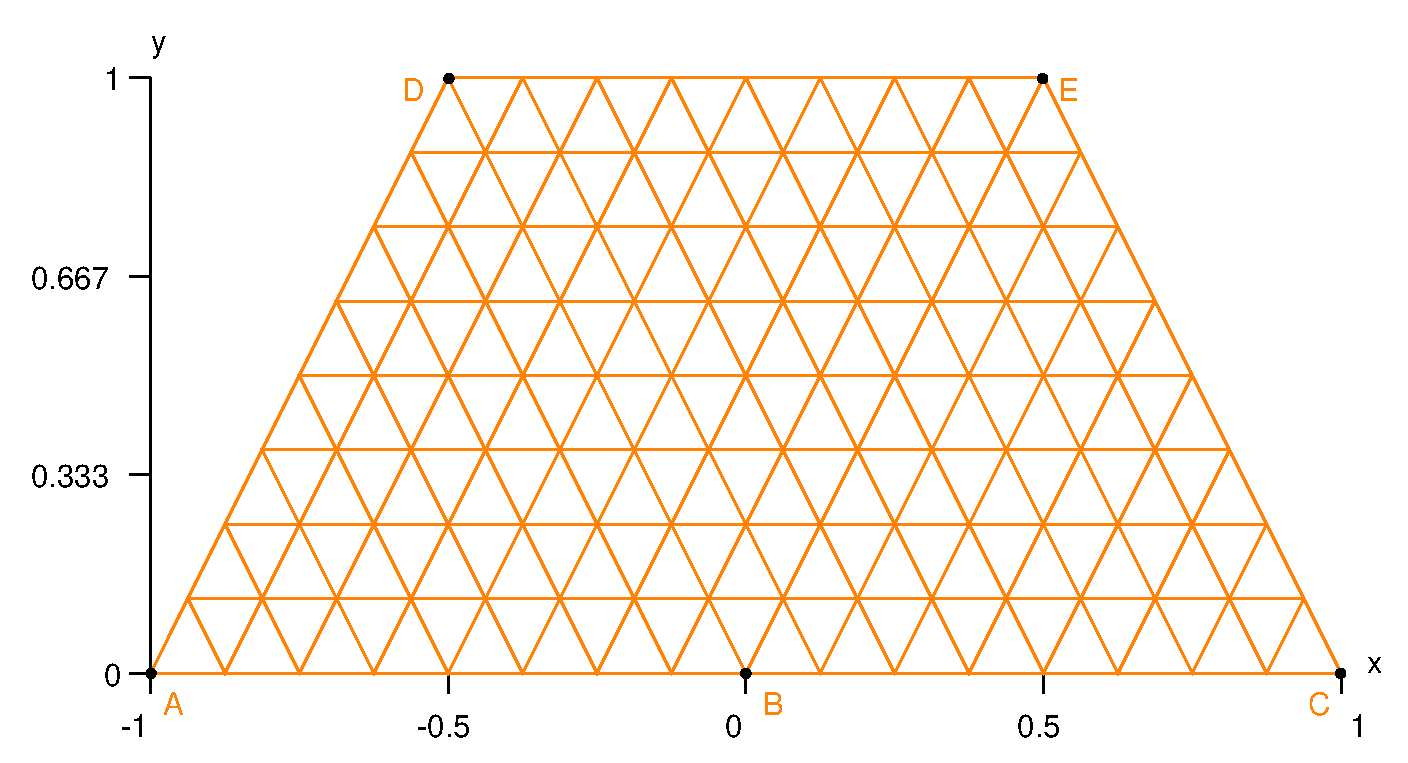
\includegraphics[width=90mm]{three-tri}
  \caption{Mesh obtained by {\small\tt join}ing three triangles}
  \label{\numb section 1.\numb fig 7}
\end{figure}

\begin{Verbatim}[commandchars=\\\{\},formatcom=\small\tt,frame=single,
   label=parag-\ref{\numb section 1.\numb parag 5}.cpp,rulecolor=\color{moldura},
   baselinestretch=0.94,framesep=2mm]
   \verm{Cell} \azul{A} ( \textcolor{tag}{tag}::vertex );  x(A) = \laranja{-1.} ;  y(A) = \laranja{0.};
   \verm{Cell} \azul{B} ( \textcolor{tag}{tag}::vertex );  x(B) =  \laranja{0.} ;  y(B) = \laranja{0.};
   \verm{Cell} \azul{C} ( \textcolor{tag}{tag}::vertex );  x(C) =  \laranja{1.} ;  y(C) = \laranja{0.};
   \verm{Cell} \azul{D} ( \textcolor{tag}{tag}::vertex );  x(D) = \laranja{-0.5};  y(D) = \laranja{1.};
   \verm{Cell} \azul{E} ( \textcolor{tag}{tag}::vertex );  x(E) =  \laranja{0.5};  y(E) = \laranja{1.};

   \verm{Mesh} \azul{AB} ( \textcolor{tag}{tag}::segment, A .reverse(), B, \textcolor{tag}{tag}::divided_in, \laranja{8} );
   \verm{Mesh} \azul{BC} ( \textcolor{tag}{tag}::segment, B .reverse(), C, \textcolor{tag}{tag}::divided_in, \laranja{8} );
   \verm{Mesh} \azul{AD} ( \textcolor{tag}{tag}::segment, A .reverse(), D, \textcolor{tag}{tag}::divided_in, \laranja{8} );
   \verm{Mesh} \azul{BD} ( \textcolor{tag}{tag}::segment, B .reverse(), D, \textcolor{tag}{tag}::divided_in, \laranja{8} );
   \verm{Mesh} \azul{BE} ( \textcolor{tag}{tag}::segment, B .reverse(), E, \textcolor{tag}{tag}::divided_in, \laranja{8} );
   \verm{Mesh} \azul{CE} ( \textcolor{tag}{tag}::segment, C .reverse(), E, \textcolor{tag}{tag}::divided_in, \laranja{8} );
   \verm{Mesh} \azul{ED} ( \textcolor{tag}{tag}::segment, E .reverse(), D, \textcolor{tag}{tag}::divided_in, \laranja{8} );

   \verm{Mesh} \azul{ABD} ( \textcolor{tag}{tag}::triangle, AB, BD, AD .reverse() );
   \verm{Mesh} \azul{BCE} ( \textcolor{tag}{tag}::triangle, BC, CE, BE .reverse() );
   \verm{Mesh} \azul{BED} ( \textcolor{tag}{tag}::triangle, BE, ED, BD .reverse() );

   \verm{Mesh} \azul{three_tri} ( \textcolor{tag}{tag}::join, ABD, BCE, BED );
\end{Verbatim}


          %-------------------------------%
\section{~~Mixing triangles and rectangles}\label{\numb section 1.\numb parag 6}
          %-------------------------------%

It is possible to have triangles and quadrilaterals mixed in the same mesh :

\begin{Verbatim}[commandchars=\\\{\},formatcom=\small\tt,frame=single,
   label=parag-\ref{\numb section 1.\numb parag 6}.cpp,rulecolor=\color{moldura},
   baselinestretch=0.94,framesep=2mm]
   \verm{Mesh} \azul{ABD} ( \textcolor{tag}{tag}::triangle, AB, BD, AD .reverse() );
   \verm{Mesh} \azul{BCE} ( \textcolor{tag}{tag}::triangle, BC, CE, BE .reverse() );
   \verm{Mesh} \azul{BEFD} ( \textcolor{tag}{tag}::quadrangle, BE, EF, FD, BD .reverse() );
   \verm{Mesh} \azul{two_tri_one_rect} ( \textcolor{tag}{tag}::join, ABD, BEFD, BCE );
\end{Verbatim}

\begin{figure}[ht] \centering
  \psfrag{A}{\small\tt\textcolor{textindraw}{A}}
  \psfrag{B}{\small\tt\textcolor{textindraw}{B}}
  \psfrag{C}{\small\tt\textcolor{textindraw}{C}}
  \psfrag{D}{\small\tt\textcolor{textindraw}{D}}
  \psfrag{E}{\small\tt\textcolor{textindraw}{E}}
  \psfrag{F}{\small\tt\textcolor{textindraw}{F}}
  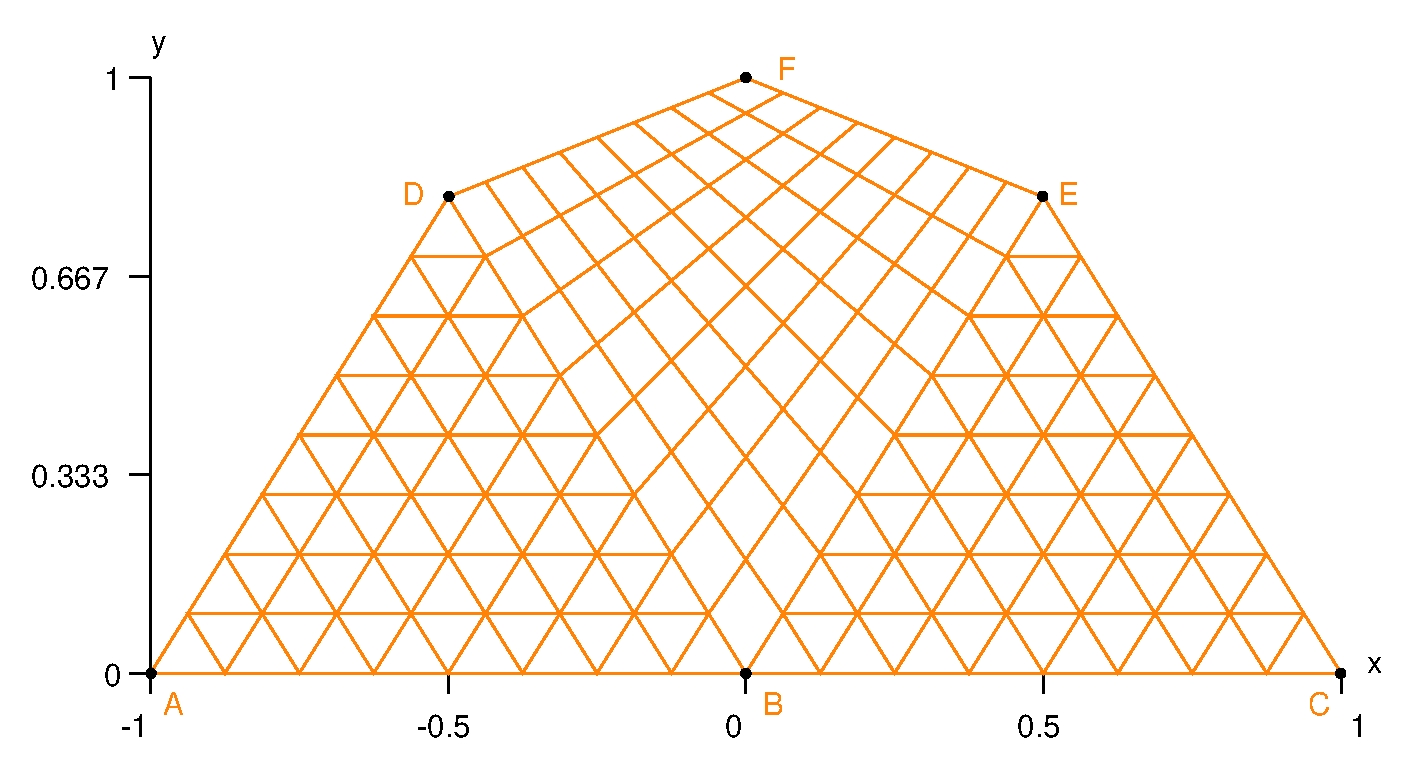
\includegraphics[width=110mm]{two-tri-one-rect}
  \caption{Mixed mesh}
  \label{\numb section 1.\numb fig 8}
\end{figure}

The resulting mesh is shown in figure \ref{\numb section 1.\numb fig 8}.

Paragraphs \ref{\numb section 2.\numb parag 2} and \ref{\numb section 2.\numb parag 3}
show other examples of mixed meshes.


          %--------------%
\section{~~Meshing a cube}\label{\numb section 1.\numb parag 7}
          %--------------%

To build a mesh of cubic cells, we first build eight vertices, then twelve segments,
then six squares, then finally invoke the {\small\tt\verm{Mesh}} constructor with
{\small\tt\textcolor{tag}{tag}::cube} (or, equivalently,
{\small\tt\textcolor{tag}{tag}::hexahedron})

\begin{Verbatim}[commandchars=\\\{\},formatcom=\small\tt,frame=single,
   label=parag-\ref{\numb section 1.\numb parag 7}.cpp,rulecolor=\color{moldura},
   baselinestretch=0.94,framesep=2mm]
   \verm{Mesh} \azul{cube} ( \textcolor{tag}{tag}::cube, ABCD, HGFE, BFGC, DHEA, CGHD, AEFB );
\end{Verbatim}

\begin{figure}[ht] \centering
  \psfrag{A}{\small\tt\textcolor{textindraw}{A}}
  \psfrag{B}{\small\tt\textcolor{textindraw}{B}}
  \psfrag{C}{\small\tt\textcolor{textindraw}{C}}
  \psfrag{D}{\small\tt\textcolor{textindraw}{D}}
  \psfrag{E}{\small\tt\textcolor{textindraw}{E}}
  \psfrag{F}{\small\tt\textcolor{textindraw}{F}}
  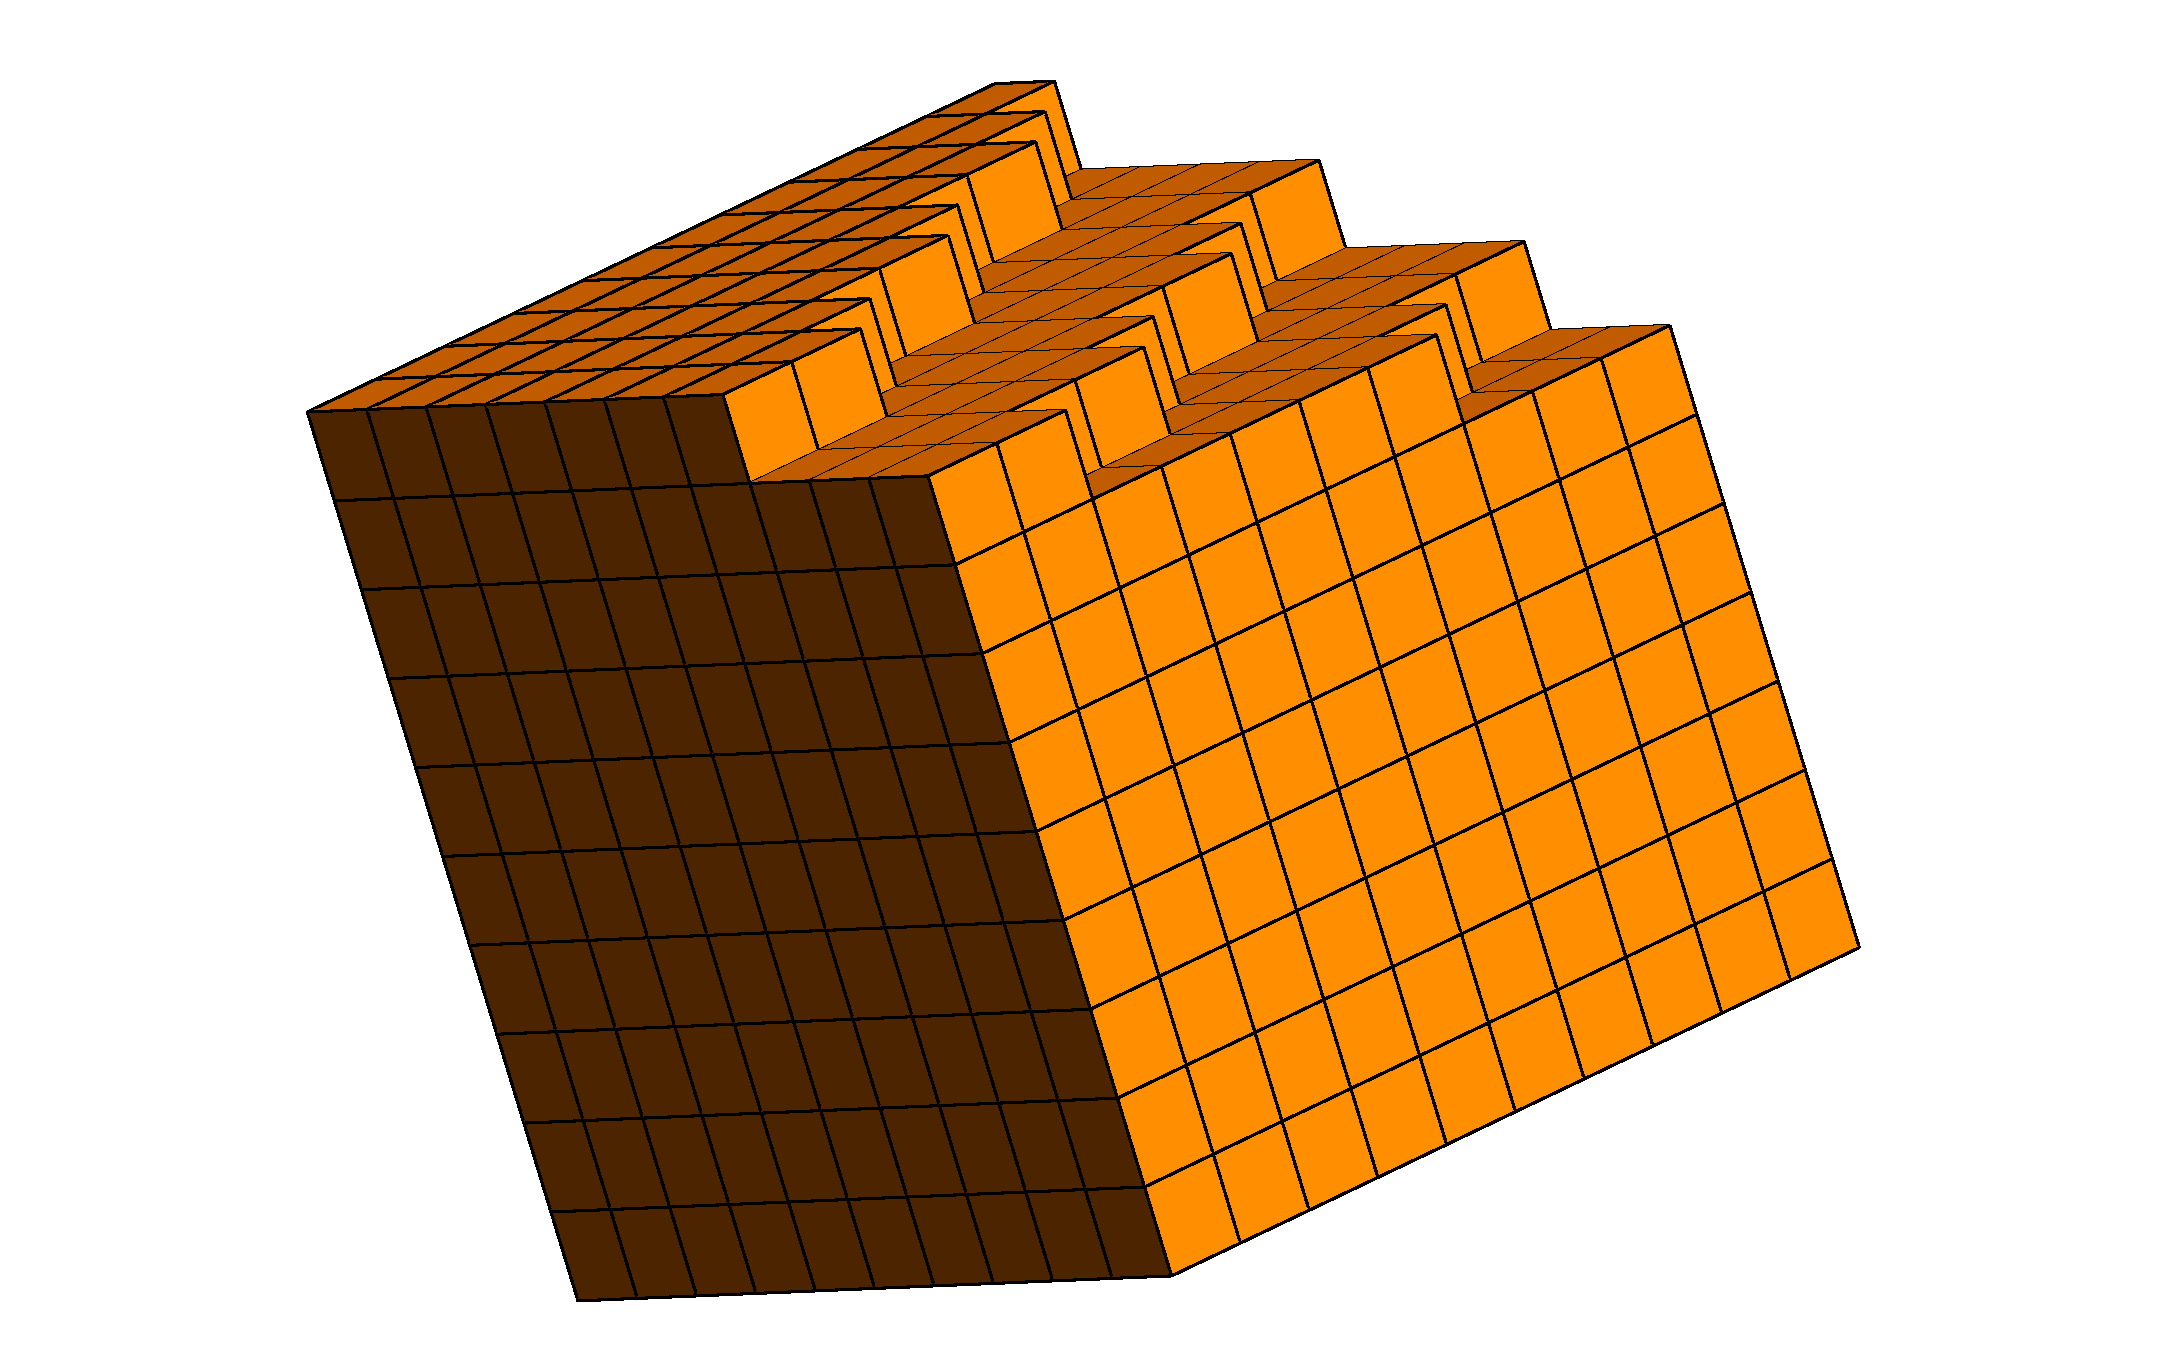
\includegraphics[width=110mm]{cube-cut}
  \caption{Mesh of cubes}
  \label{\numb section 1.\numb fig 9}
\end{figure}


Just like for two-dimensional rectangular meshes, the orientation of the resulting mesh is determined
by the orientation of the six faces, as provided by the user.
These orientations must be mutually compatible.

The order of the arguments of the above {\small\tt\verm{Mesh}} constructor is not rigid;
the only constraint is that the first two meshes provided should be opposite faces of the cube,
just like the third and the fourth and the last two.

In figure \ref{\numb section 1.\numb fig 9}, some cells have been removed so that the reader
can see the inside of the cube.
This was done using the following options of {\small\tt gmsh}: {\small\tt Tools} $\to$
{\small\tt Clipping} $\to$ {\small\tt Mesh} $\to$ {\small\tt Planes} $\to$
{\small\tt Keep whole elements}, $ A = 1, B = -0.2, C = -0.3, D = 0.1 $.

Just like for two-dimensional rectangular meshes, vertices may be in any position in the space,
the space may have more than three dimensions, edges and faces may be curved.
Paragraphs \ref{\numb section 2.\numb parag 13} and \ref{\numb section 2.\numb parag 16} show a
fancier use of the {\small\tt\verm{Mesh}} constructor with {\small\tt\textcolor{tag}{tag}::cube}.





          %------------------------------%
\section{~~Similar products (competitors)}\label{\numb section 1.\numb parag 8}
          %------------------------------%

deal.II : {\small\tt https://dealii.org/}

FEniCS/ Dolphin : {\small\tt https://fenicsproject.org/}

FreeFem++ : {\small\tt http://www3.freefem.org/}

GetFEM : {\small\tt https://getfem.org/download.html}

gmsh : {\small\tt http://gmsh.info}

MFEM : {\small\tt https://opensourcelibs.com/lib/mfem}

OFELI : {\small\tt http://ofeli.org/}

PETSc-FEM : {\small\tt https://cimec.org.ar/foswiki/Main/Cimec/PETScFEM}

PolyFEM : {\small\tt https://github.com/polyfem/polyfem}


          %-------------%
\section{~~Strong points}\label{\numb section 1.\numb parag 9}
          %-------------%

{\ManiFEM} offers a flexible and general approach for defining meshes on manifolds
(sections \ref{\numb section 2} and \ref{\numb section 3}).
Meshes on quotient manifolds (section \ref{\numb section 7}) are handy for solving
problems with periodic boundary conditions.

One of the goals of {\maniFEM} is to make remeshing easy for end users.
Thus, meshes can be manipulated (cells can be added and removed) using intuitive commands
(section \ref{\numb section 10}).

In {\maniFEM}, the user defines finite elements using a clear and intuitive syntax
(section \ref{\numb section 6}).
Some types of finite elements are rather slow; they are interesting for dydactic purposes.
Fast versions are available; they use a slightly less clear syntax.

The manual is clear and presents many examples.


          %-----------%
\section{~~Weak points}\label{\numb section 1.\numb parag 10}
          %-----------%

{\ManiFEM} is not ready for parallel processing.

Some finite elements are slow (but fast versions are available).

Since {\maniFEM} is under heavy development, some features are still missing,
e.g.\ 3D frontal meshing, many types of finite elements, compact syntax for abstract variational
formulations.
See the changelog at the end of this manual (just before the index), especially the ``To do''
paragraph.

{\ManiFEM} relies on oriented cells and meshes.
Some people may find it confusing (the distinction between positive cells and negative cells).


          %--------------------%
\chapter{~~Meshes and manifolds; patchwork}\label{\numb section 2}
          %--------------------%

This section describes several examples of meshes, some of them built on specific manifolds.
Note that in this manual we use the term ``manifold'' to mean a manifold without boundary.

This section focuses on building meshes by joining together several regular meshes
(triangles or quadrangles), like patches.
In contrast, section \ref{\numb section 3} shows how to mesh regions of a manifold
by progressively adding triangular cells, one by one.

Paragraphs \ref{\numb section 2.\numb parag 4}, \ref{\numb section 2.\numb parag 5},
\ref{\numb section 2.\numb parag 9} and \ref{\numb section 2.\numb parag 11} deal
with one-dimensional meshes (curves) in $ \mathbb{R}^2 $,
paragraphs \ref{\numb section 2.\numb parag 13}, \ref{\numb section 2.\numb parag 14},
\ref{\numb section 2.\numb parag 15} and \ref{\numb section 2.\numb parag 16} show
curves in $ \mathbb{R}^3 $,
paragraphs \ref{\numb section 2.\numb parag 1}, \ref{\numb section 2.\numb parag 2},
\ref{\numb section 2.\numb parag 3}, \ref{\numb section 2.\numb parag 9} and
\ref{\numb section 2.\numb parag 11} show plane domains
(two-dimensional meshes in $ \mathbb{R}^2 $),
while paragraphs \ref{\numb section 2.\numb parag 6}, \ref{\numb section 2.\numb parag 7},
\ref{\numb section 2.\numb parag 8}, \ref{\numb section 2.\numb parag 13},
\ref{\numb section 2.\numb parag 14}, \ref{\numb section 2.\numb parag 17} and
\ref{\numb section 2.\numb parag 18} focus on two-dimensional meshes
in $ \mathbb{R}^3 $ (surfaces).

Paragraphs \ref{\numb section 2.\numb parag 4} -- \ref{\numb section 2.\numb parag 14}
are about manifolds defined implicitly as level sets;
paragraphs \ref{\numb section 2.\numb parag 15} -- \ref{\numb section 2.\numb parag 18}
describe parametric manifolds.


          %----------------%
\section{~~Joining segments}\label{\numb section 2.\numb parag 1}
          %----------------%

Here is another way of meshing the same L-shaped domain as in paragraph
\ref{\numb section 1.\numb parag 4} :

\begin{figure}[ht] \centering
  \psfrag{A}{\small\tt\textcolor{textindraw}{A}}
  \psfrag{B}{\small\tt\textcolor{textindraw}{B}}
  \psfrag{C}{\small\tt\textcolor{textindraw}{C}}
  \psfrag{D}{\small\tt\textcolor{textindraw}{D}}
  \psfrag{E}{\small\tt\textcolor{textindraw}{E}}
  \psfrag{F}{\small\tt\textcolor{textindraw}{F}}
  \psfrag{G}{\small\tt\textcolor{textindraw}{G}}
  \psfrag{H}{\small\tt\textcolor{textindraw}{H}}
  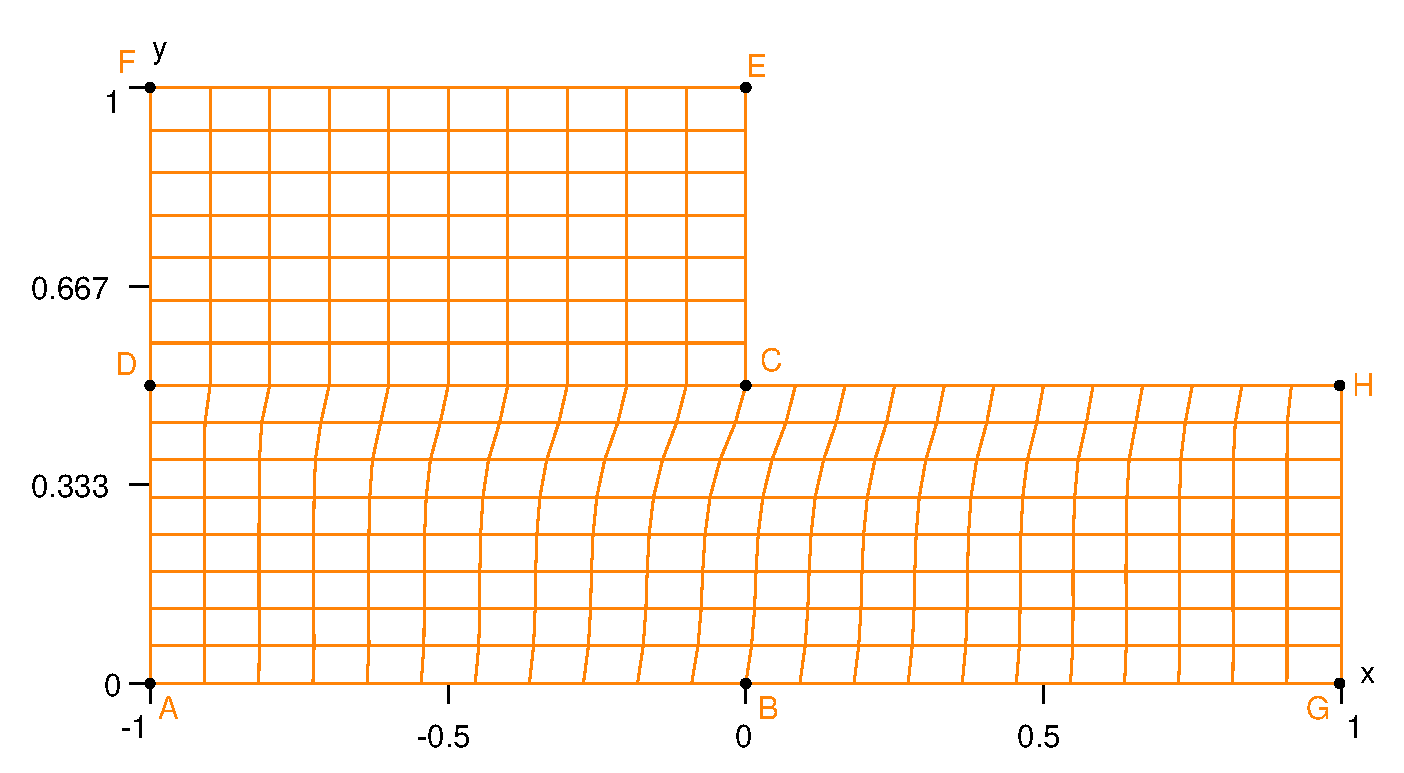
\includegraphics[width=95mm]{L-shaped-distorted}
  \caption{An L-shaped mesh again}
  \label{\numb section 2.\numb fig 1}
\end{figure}

\begin{Verbatim}[commandchars=\\\{\},formatcom=\small\tt,frame=single,
   label=parag-\ref{\numb section 2.\numb parag 1}.cpp,rulecolor=\color{coment},
   baselinestretch=0.94,framesep=2mm]
   \verm{Mesh} \azul{AG} ( \textcolor{tag}{tag}::segment, A .reverse(), G, \textcolor{tag}{tag}::divided_in, \laranja{22} );
   \verm{Mesh} \azul{GH} ( \textcolor{tag}{tag}::segment, G .reverse(), H, \textcolor{tag}{tag}::divided_in,  \laranja{8} );
   \verm{Mesh} \azul{HC} ( \textcolor{tag}{tag}::segment, H .reverse(), C, \textcolor{tag}{tag}::divided_in, \laranja{12} );
   \verm{Mesh} \azul{CD} ( \textcolor{tag}{tag}::segment, C .reverse(), D, \textcolor{tag}{tag}::divided_in, \laranja{10} );
   \verm{Mesh} \azul{HD} ( \textcolor{tag}{tag}::join, HC, CD );
   \verm{Mesh} \azul{DA} ( \textcolor{tag}{tag}::segment, D .reverse(), A, \textcolor{tag}{tag}::divided_in,  \laranja{8} );
   \verm{Mesh} \azul{CE} ( \textcolor{tag}{tag}::segment, C .reverse(), E, \textcolor{tag}{tag}::divided_in,  \laranja{7} );
   \verm{Mesh} \azul{EF} ( \textcolor{tag}{tag}::segment, E .reverse(), F, \textcolor{tag}{tag}::divided_in, \laranja{10} );
   \verm{Mesh} \azul{FD} ( \textcolor{tag}{tag}::segment, F .reverse(), D, \textcolor{tag}{tag}::divided_in,  \laranja{7} );
   \verm{Mesh} \azul{AGHD} ( \textcolor{tag}{tag}::rectangle, AG, GH, HD, DA );
   \verm{Mesh} \azul{CEFD} ( \textcolor{tag}{tag}::rectangle, CE, EF, FD, CD .reverse() );
   \verm{Mesh} \azul{L_shaped} ( \textcolor{tag}{tag}::join, AGHD, CEFD );
\end{Verbatim}

The only difference between this mesh and the one presented in paragraph
\ref{\numb section 1.\numb parag 4} is a slight distortion in the lower half of the domain,
due to the non-uniform distribution of the vertices along {\small\tt HD}.

Paragraph \ref{\numb section 11.\numb parag 2} explains the coloring conventions used in
this manual for {\tt C++} code.
Paragraph \ref{\numb section 11.\numb parag 3} gives details about \textcolor{tag}{tag}s.


          %---------%
\section{~~Exercise}\label{\numb section 2.\numb parag 2}
          %---------%

Build the mesh shown in figure \ref{\numb section 2.\numb fig 2}.
We ask for one connected mesh, that is, the triangle and the rectangle must share some vertices
(and segments, reversed).

\begin{figure}[ht] \centering
  \psfrag{A}{\small\tt\textcolor{textindraw}{A}}
  \psfrag{B}{\small\tt\textcolor{textindraw}{B}}
  \psfrag{C}{\small\tt\textcolor{textindraw}{C}}
  \psfrag{D}{\small\tt\textcolor{textindraw}{D}}
  \psfrag{E}{\small\tt\textcolor{textindraw}{E}}
  \psfrag{F}{\small\tt\textcolor{textindraw}{F}}
  \psfrag{G}{\small\tt\textcolor{textindraw}{G}}
  \psfrag{H}{\small\tt\textcolor{textindraw}{H}}
  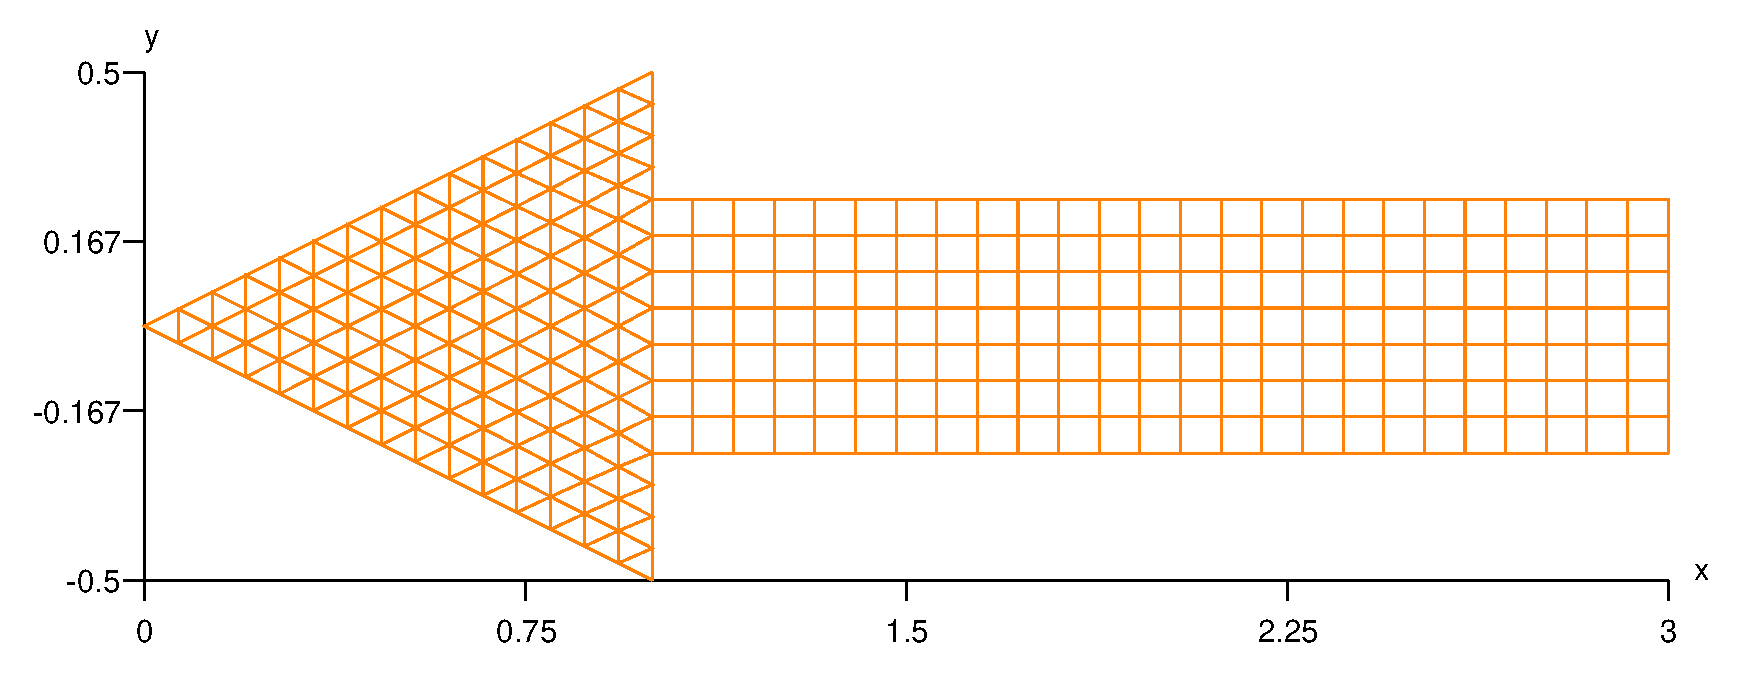
\includegraphics[width=130mm]{arrow}
  \caption{An arrow}
  \label{\numb section 2.\numb fig 2}
\end{figure}


          %-------------------------------%
\section{~~Triangular meshes on rectangles}\label{\numb section 2.\numb parag 3}
          %-------------------------------%

On a rectangular domain, we can build a mesh of triangles by using the {\small\tt\verm{Mesh}}
constructor with {\small\tt\textcolor{tag}{tag}::rectangle}, providing as last argument the
{\small\tt\textcolor{tag}{tag}::with\_\,triangles}.
For instance, in the example \ref{\numb section 1.\numb parag 4},
if we re-write the definition of {\small\tt BGHC} as

\begin{Verbatim}[commandchars=\\\{\},formatcom=\small\tt,baselinestretch=0.94]
   \verm{Mesh} \azul{BGHC} ( \textcolor{tag}{tag}::rectangle, BG, GH, HC, BC .reverse(), \textcolor{tag}{tag}::with_triangles );
\end{Verbatim}

\noindent we get the mesh shown in figure \ref{\numb section 2.\numb fig 3}.

\begin{figure}[ht] \centering
  \psfrag{A}{\small\tt\textcolor{textindraw}{A}}
  \psfrag{B}{\small\tt\textcolor{textindraw}{B}}
  \psfrag{C}{\small\tt\textcolor{textindraw}{C}}
  \psfrag{D}{\small\tt\textcolor{textindraw}{D}}
  \psfrag{E}{\small\tt\textcolor{textindraw}{E}}
  \psfrag{F}{\small\tt\textcolor{textindraw}{F}}
  \psfrag{G}{\small\tt\textcolor{textindraw}{G}}
  \psfrag{H}{\small\tt\textcolor{textindraw}{H}}
  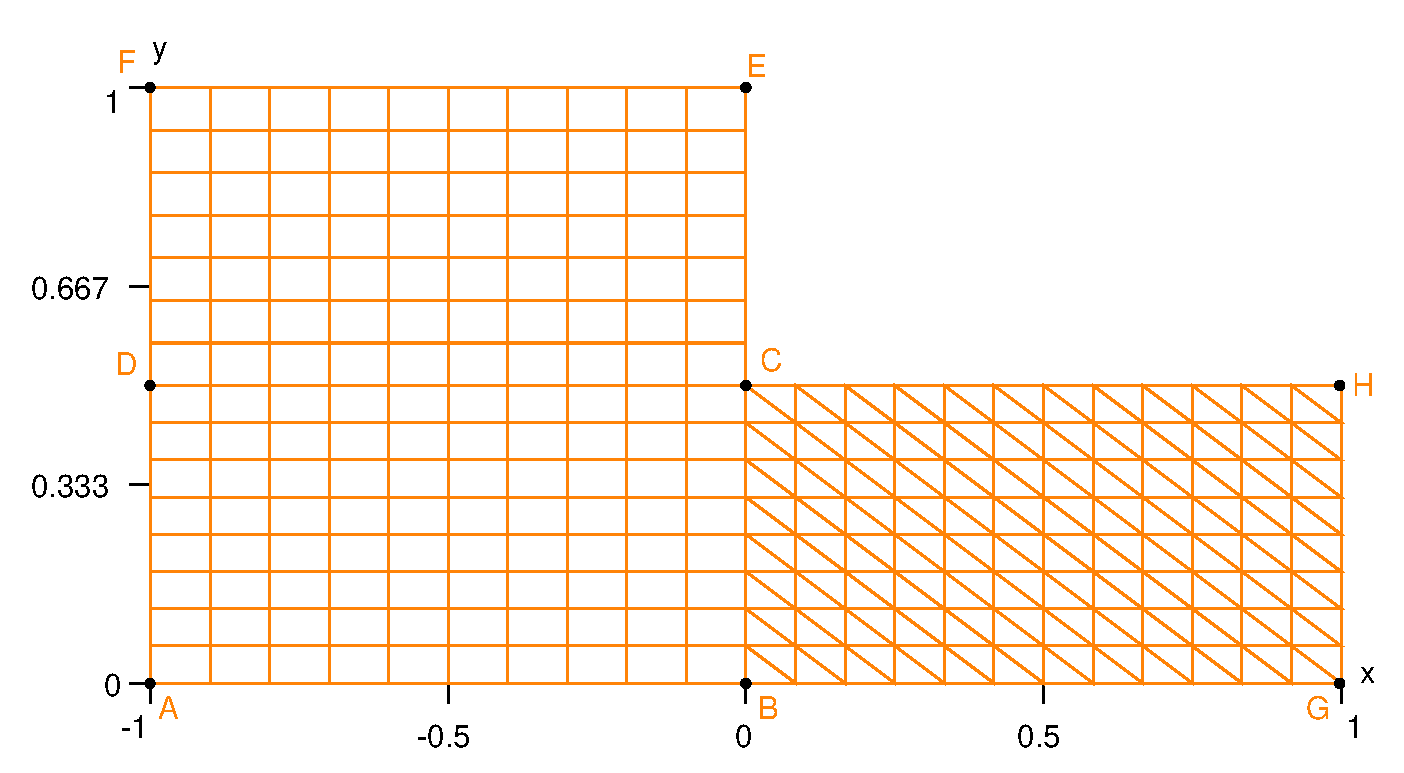
\includegraphics[width=108mm]{L-shaped-tri}
  \caption{An L-shaped mesh with triangular cells}
  \label{\numb section 2.\numb fig 3}
\end{figure}

If we give the sides of the rectangle in a different order, like in

\begin{Verbatim}[commandchars=\\\{\},formatcom=\small\tt,baselinestretch=0.94]
   \verm{Mesh} \azul{BGHC} ( \textcolor{tag}{tag}::rectangle, GH, HC, BC .reverse(), BG, \textcolor{tag}{tag}::with_triangles );
\end{Verbatim}

\noindent the rectangles will be cut along the other diagonal (check it yourself).

The mesh in paragraph \ref{\numb section 1.\numb parag 5} could have been built like this :

\begin{Verbatim}[commandchars=\\\{\},formatcom=\small\tt,baselinestretch=0.94]
   \verm{Mesh} \azul{ABD} ( \textcolor{tag}{tag}::triangle, AB, BD, AD .reverse() );
   \verm{Mesh} \azul{BCED} ( \textcolor{tag}{tag}::quadrangle, CE, ED, BD .reverse(), BC, \textcolor{tag}{tag}::with_triangles );
   \verm{Mesh} \azul{one_tri_one_rect} ( \textcolor{tag}{tag}::join, ABD, BCED );
\end{Verbatim}


          %-----------------------------------------------------%
\section{~~A manifold defined as a level set in $ \mathbb{R}^2 $}
          %-----------------------------------------------------%
\label{\numb section 2.\numb parag 4}

{\ManiFEM} allows one to define manifolds and submanifolds, and this feature may be
used to build domains of the desired shape.

Until now, we have only met the trivial Euclidian manifold, defined as {\small\tt
\verm{Manifold}\break ( \textcolor{tag}{tag}::Euclid,} {\small\tt\textcolor{tag}{tag}::of\_\,dim,}
{\small\tt n} {\small\tt )}.
One can define a submanifold in terms of an implicit equation, that is, as a level set,
using the method {\small\tt implicit} of the Euclidian manifold.
The code below introduces a one-dimensional submanifold of $ \mathbb{R}^2 $ (a hiperbola).

\begin{Verbatim}[commandchars=\\\{\},formatcom=\small\tt,frame=single,
   label=parag-\ref{\numb section 2.\numb parag 4}.cpp,rulecolor=\color{coment},
   baselinestretch=0.94,framesep=2mm]
   \verm{Manifold} \azul{RR2} ( \textcolor{tag}{tag}::Euclid, \textcolor{tag}{tag}::of_dim, \laranja{2} );
   \verm{Function} \azul{xy} = RR2 .build_coordinate_system ( \textcolor{tag}{tag}::Lagrange, \textcolor{tag}{tag}::of_degree, \laranja{1} );
   \verm{Function} \azul{x} = xy [\laranja{0}], \azul{y} = xy [\laranja{1}];
   
   \verm{Manifold} \azul{hiperbola} = RR2 .implicit ( x*y == \laranja{1.} );
   
   \verm{Cell} \azul{A} ( \textcolor{tag}{tag}::vertex );  x (A) =  \laranja{0.5};   y (A) =  \laranja{2.};
   \verm{Cell} \azul{B} ( \textcolor{tag}{tag}::vertex );  x (B) =  \laranja{3};     y (B) =  \laranja{0.333333333333};
   \verm{Mesh} \azul{arc_of_hiperbola} ( \textcolor{tag}{tag}::segment, A .reverse(), B, \textcolor{tag}{tag}::divided_in, \laranja{7} );
   arc_of_hiperbola .draw_ps (\verde{"hiperbola.eps"});
   arc_of_hiperbola .export_to_file ( \textcolor{tag}{tag}::msh, \verde{"hiperbola.msh"});
\end{Verbatim}

\begin{figure}[ht] \centering
  \psfrag{A}{\small\tt\textcolor{textindraw}{A}}
  \psfrag{B}{\small\tt\textcolor{textindraw}{B}}
  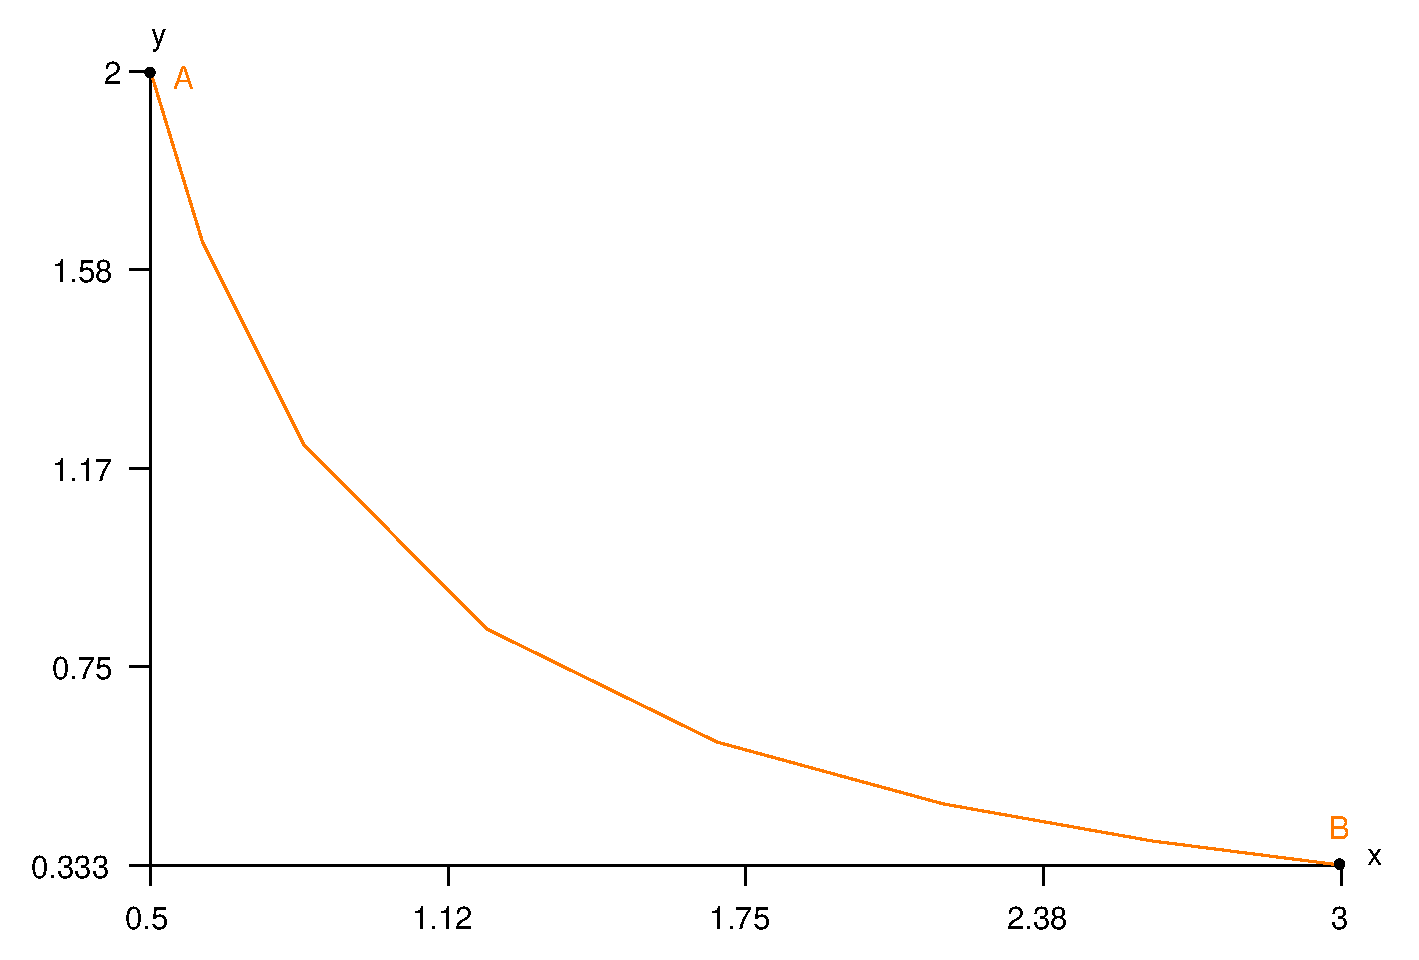
\includegraphics[width=85mm]{hiperbola}
  \caption{An arc of hiperbola}
  \label{\numb section 2.\numb fig 4}
\end{figure}

In {\tt gmsh}, you must select {\small\tt Tools} $\to$ {\small\tt Options} $\to$
{\small\tt Mesh} $\to$ {\small\tt 1D Elements} in order to see this mesh.

Note that the vertices are not perfectly uniformly distributed along the curve
because they are obtained as projections of points uniformly distributed along
the straight segment {\small\tt AB} onto the {\small\tt hiperbola} manifold.

Note also that when defining individual points {\small\tt A} and {\small\tt B} we must
be careful to set coordinates {\small\tt x} and {\small\tt y} within
the {\small\tt hiperbola} manifold.
As an alternative, we might explicitly project them onto the {\small\tt hiperbola} like this :

\begin{Verbatim}[commandchars=\\\{\},formatcom=\small\tt,baselinestretch=0.94]
   \verm{Cell} \azul{P} ( \textcolor{tag}{tag}::vertex );  x (P) = \laranja{0.6};  y (P) = \laranja{2.1};
   hiperbola .project (P);
\end{Verbatim}

\noindent In contrast, the {\small\tt\verm{Mesh}} constructor with
{\small\tt\textcolor{tag}{tag}::segment} builds points in the surrounding space {\small\tt RR2}
and then projects them onto the {\small\tt hiperbola} without the user's assistance.

The projection is done by applying a few steps of Newton's method for under-determined
(systems of) equations, as explained in paragraph \ref{\numb section 8.\numb parag 1}.

Paragraph \ref{\numb section 3.\numb parag 5} shows another way of meshing a curve,
producing equidistant vertices.


          %----------------------------------------%
\section{~~A circle defined by four curved segments}\label{\numb section 2.\numb parag 5}
          %----------------------------------------%

We can define several arcs of curve and {\small\tt join} them, thus obtaining a closed curve :
\medskip

\begin{Verbatim}[commandchars=\\\{\},formatcom=\small\tt,frame=single,
   label=parag-\ref{\numb section 2.\numb parag 5}.cpp,rulecolor=\color{coment},
   baselinestretch=0.94,framesep=2mm]
   \verm{Cell} \azul{N} ( \textcolor{tag}{tag}::vertex );  x (N) =  \laranja{0.};  y (N) =  \laranja{1.};
   \verm{Cell} \azul{W} ( \textcolor{tag}{tag}::vertex );  x (W) = \laranja{-1.};  y (W) =  \laranja{0.};
   \verm{Cell} \azul{S} ( \textcolor{tag}{tag}::vertex );  x (S) =  \laranja{0.};  y (S) = \laranja{-1.};
   \verm{Cell} \azul{E} ( \textcolor{tag}{tag}::vertex );  x (E) =  \laranja{1.};  y (E) =  \laranja{0.};
   \verm{Mesh} \azul{NW} ( \textcolor{tag}{tag}::segment, N .reverse(), W, \textcolor{tag}{tag}::divided_in, \laranja{5} );
   \verm{Mesh} \azul{WS} ( \textcolor{tag}{tag}::segment, W .reverse(), S, \textcolor{tag}{tag}::divided_in, \laranja{5} );
   \verm{Mesh} \azul{SE} ( \textcolor{tag}{tag}::segment, S .reverse(), E, \textcolor{tag}{tag}::divided_in, \laranja{5} );
   \verm{Mesh} \azul{EN} ( \textcolor{tag}{tag}::segment, E .reverse(), N, \textcolor{tag}{tag}::divided_in, \laranja{5} );
   \verm{Mesh} \azul{circle} ( \textcolor{tag}{tag}::join, NW, WS, SE, EN );
\end{Verbatim}

\begin{figure}[ht] \centering
  \psfrag{N}{\small\tt\textcolor{textindraw}{N}}
  \psfrag{S}{\small\tt\textcolor{textindraw}{S}}
  \psfrag{E}{\small\tt\textcolor{textindraw}{E}}
  \psfrag{W}{\small\tt\textcolor{textindraw}{W}}
  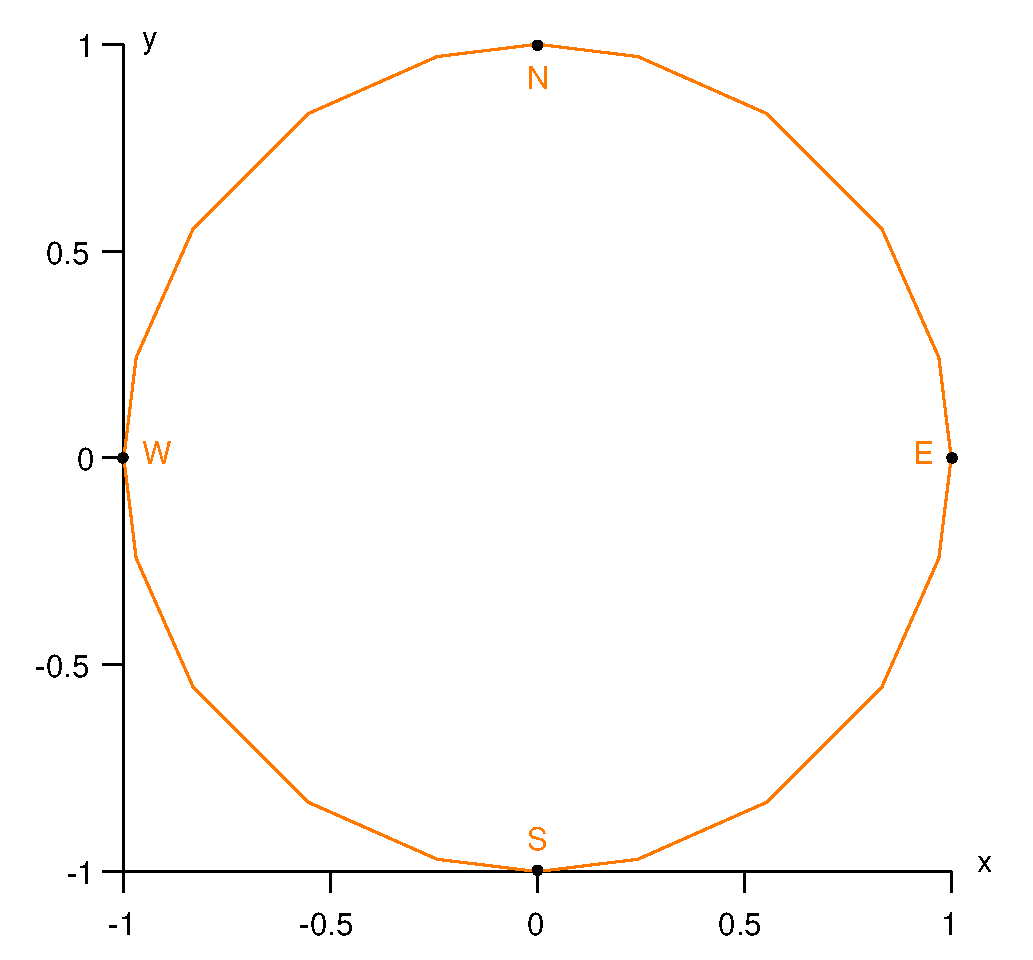
\includegraphics[width=70mm]{circle}
  \caption{A circle obtained by {\small\tt join}ing four segments}
  \label{\numb section 2.\numb fig 5}
\end{figure}

Again, the distribution of vertices along the circle is not perfect
because vertices are obtained as projections (on the circle) of points
along straight segments {\small\tt NW}, {\small\tt WS} and so forth.
Paragraph \ref{\numb section 3.\numb parag 2} shows another way of meshing a closed curve,
producing equidistant vertices.

Note that applying the {\small\tt\verm{Mesh}} constructor with {\small\tt\textcolor{tag}{tag}::join}
to four segments is very different from applying the {\small\tt\verm{Mesh}} constructor with
{\small\tt\textcolor{tag}{tag}::quadrangle} to the same four segments;
see paragraphs \ref{\numb section 2.\numb parag 9} and \ref{\numb section 2.\numb parag 11}.


          %---------------------------------------------%
\section{~~A hemisphere defined by four curved triangles}\label{\numb section 2.\numb parag 6}
          %---------------------------------------------%

Let's look at a surface in $ \mathbb{R}^3 $ :

\begin{Verbatim}[commandchars=\\\{\},formatcom=\small\tt,frame=single,
   label=parag-\ref{\numb section 2.\numb parag 6}.cpp,rulecolor=\color{coment},
   baselinestretch=0.94,framesep=2mm                                            ]
   \verm{Manifold} \azul{RR3} ( \textcolor{tag}{tag}::Euclid, \textcolor{tag}{tag}::of_dim, \laranja{3} );
   \verm{Function} \azul{xyz} = RR3 .build_coordinate_system ( \textcolor{tag}{tag}::Lagrange, \textcolor{tag}{tag}::of_degree, \laranja{1} );
   \verm{Function} \azul{x} = xyz [\laranja{0}], \azul{y} = xyz [\laranja{1}], \azul{z} = xyz [\laranja{2}];

   \verm{Manifold} \azul{sphere} = RR3 .implicit ( x*x + y*y + z*z == \laranja{1.} );

   \cinza{// let's mesh half of a sphere}
   \verm{Cell} \azul{E}  ( \textcolor{tag}{tag}::vertex );  x (E) =  \laranja{1.};  y (E) =  \laranja{0.};  z (E) = \laranja{0.};
   \verm{Cell} \azul{N}  ( \textcolor{tag}{tag}::vertex );  x (N) =  \laranja{0.};  y (N) =  \laranja{1.};  z (N) = \laranja{0.};
   \verm{Cell} \azul{W}  ( \textcolor{tag}{tag}::vertex );  x (W) = \laranja{-1.};  y (W) =  \laranja{0.};  z (W) = \laranja{0.};
   \verm{Cell} \azul{S}  ( \textcolor{tag}{tag}::vertex );  x (W) =  \laranja{0.};  y (W) = \laranja{-1.};  z (W) = \laranja{0.};
   \verm{Cell} \azul{up} ( \textcolor{tag}{tag}::vertex );  x (up)=  \laranja{0.};  y (up)=  \laranja{0.};  z (up)= \laranja{1.};

   int \azul{n} = \laranja{15};
   \verm{Mesh} \azul{EN} ( \textcolor{tag}{tag}::segment, E .reverse(), N, \textcolor{tag}{tag}::divided_in, n );
   \verm{Mesh} \azul{NW} ( \textcolor{tag}{tag}::segment, N .reverse(), W, \textcolor{tag}{tag}::divided_in, n );
   \verm{Mesh} \azul{WS} ( \textcolor{tag}{tag}::segment, W .reverse(), S, \textcolor{tag}{tag}::divided_in, n );
   \verm{Mesh} \azul{SE} ( \textcolor{tag}{tag}::segment, S .reverse(), E, \textcolor{tag}{tag}::divided_in, n );
   \verm{Mesh} \azul{upE} ( \textcolor{tag}{tag}::segment, up .reverse(), E, \textcolor{tag}{tag}::divided_in, n );
   \verm{Mesh} \azul{upN} ( \textcolor{tag}{tag}::segment, up .reverse(), N, \textcolor{tag}{tag}::divided_in, n );
   \verm{Mesh} \azul{upW} ( \textcolor{tag}{tag}::segment, up .reverse(), W, \textcolor{tag}{tag}::divided_in, n );
   \verm{Mesh} \azul{upS} ( \textcolor{tag}{tag}::segment, up .reverse(), S, \textcolor{tag}{tag}::divided_in, n );

   \cinza{// build four triangles}
   \verm{Mesh} \azul{ENup} ( \textcolor{tag}{tag}::triangle, EN, upN .reverse(), upE );
   \verm{Mesh} \azul{NWup} ( \textcolor{tag}{tag}::triangle, NW, upW .reverse(), upN );
   \verm{Mesh} \azul{WSup} ( \textcolor{tag}{tag}::triangle, WS, upS .reverse(), upW );
   \verm{Mesh} \azul{SEup} ( \textcolor{tag}{tag}::triangle, SE, upE .reverse(), upS );

   \cinza{// and finally join the triangles :}
   \verm{Mesh} \azul{hemisphere} ( \textcolor{tag}{tag}::join, ENup, NWup, WSup, SEup );
\end{Verbatim}

\begin{figure}[ht] \centering
  \psfrag{S}{\small\tt\textcolor{textindraw}{S}}
  \psfrag{W}{\small\tt\textcolor{textindraw}{W}}
  \psfrag{up}{\small\tt\textcolor{textindraw}{up}}
  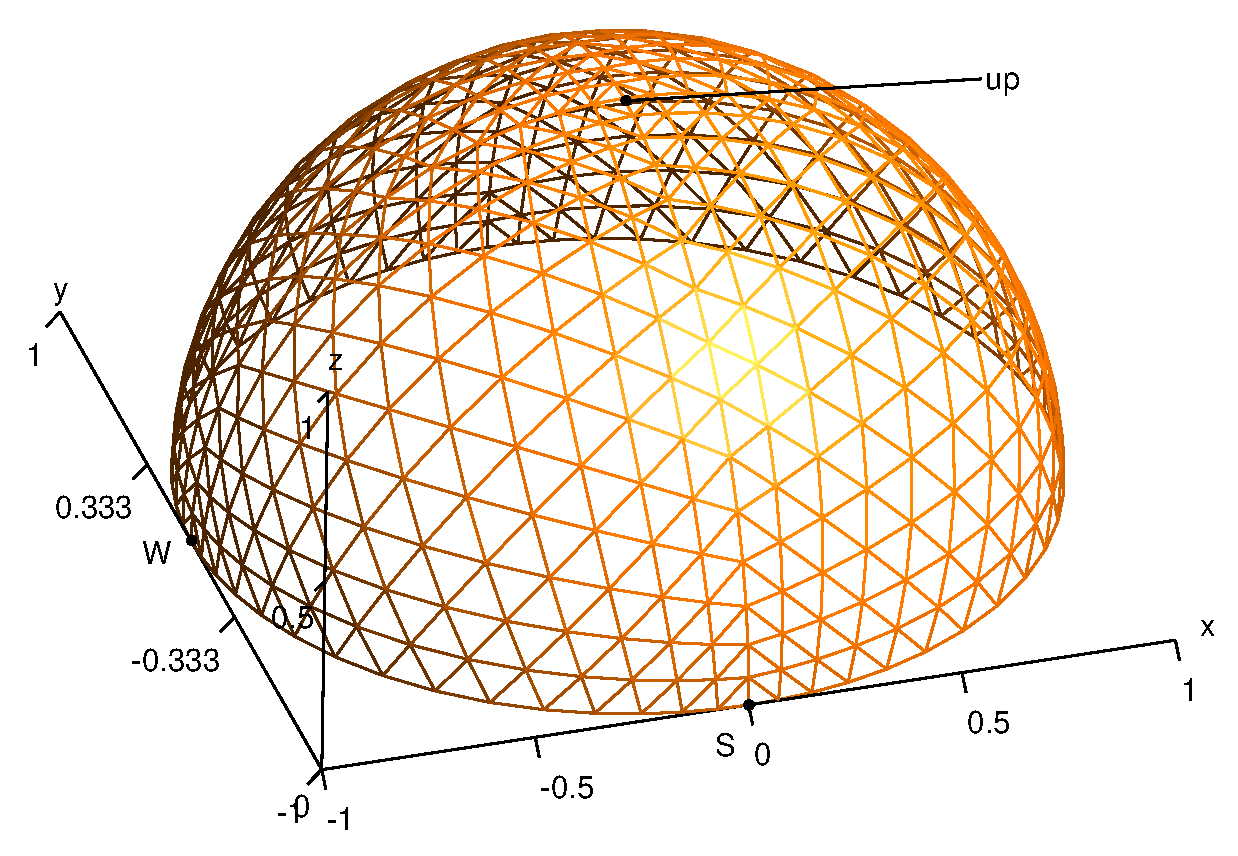
\includegraphics[width=95mm]{hemisphere}
  \caption{A hemisphere obtained by {\small\tt join}ing four triangles}
\end{figure}


Again, when we define individual points {\small\tt E}, {\small\tt N}, {\small\tt W},
{\small\tt S} and {\small\tt up} we must be careful to provide coordinates on the
{\small\tt sphere} (or {\small\tt project} them explicitly as shown in paragraph
\ref{\numb section 2.\numb parag 7}).
In contrast, the {\small\tt\verm{Mesh}} constructors with {\small\tt\textcolor{tag}{tag}::segment},
{\small\tt\textcolor{tag}{tag}::quadrangle} and {\small\tt\textcolor{tag}{tag}::triangle}
build points in the surrounding space ($ \mathbb{R}^2 $ or $ \mathbb{R}^3 $) and
then project them onto the current manifold without the user's assistance (paragraph
\ref{\numb section 8.\numb parag 1} describes this projection operation).
As a side effect, within each triangle ({\small\tt ENup}, {\small\tt NWup} and so forth),
the distribution of the vertices is not perfectly uniform.

Note that, when we build the segments {\small\tt WS}, {\small\tt upS} and so on,
we know that those segments will be (polygonal approximations of) arcs of circle on the sphere.
This is so due to the particular geometry of our manifold (we know that the projection of
a straight line segment on the sphere is an arc of circle of radius equal to the radius of
the sphere); the shape of such segments is less clear in other examples
(like the one in paragraph \ref{\numb section 2.\numb parag 7}).

Section \ref{\numb section 3} shows other ways of meshing a surface.


          %----------------------%
\section{~~A more complex surface}\label{\numb section 2.\numb parag 7}
          %----------------------%

If the surface is more ``bumpy'',
% since the projection operation doesn't work well for points far from the manifold,
we must use smaller patches in order to get a mesh of good quality.

Below we use twelve rectangles to get a bumpy hemisphere.

\begin{Verbatim}[commandchars=\\\{\},formatcom=\small\tt,frame=single,
   label=parag-\ref{\numb section 2.\numb parag 7}.cpp,rulecolor=\color{coment},
   baselinestretch=0.94,framesep=2mm]
   \verm{Manifold} nut = RR3 .implicit ( x*x + y*y + z*z + \laranja{1.5}*x*y*z == \laranja{1.} );

   \cinza{// let's mesh a hemisphere (much deformed)}
   \verm{Cell} \azul{S} ( \textcolor{tag}{tag}::vertex );   x (S)  =  \laranja{0.};  y (S)  = \laranja{-1.};  z (S)  =  \laranja{0.};
   \verm{Cell} \azul{E} ( \textcolor{tag}{tag}::vertex );   x (E)  =  \laranja{1.};  y (E)  =  \laranja{0.};  z (E)  =  \laranja{0.};
   \verm{Cell} \azul{N} ( \textcolor{tag}{tag}::vertex );   x (N)  =  \laranja{0.};  y (N)  =  \laranja{1.};  z (N)  =  \laranja{0.};
   \verm{Cell} \azul{W} ( \textcolor{tag}{tag}::vertex );   x (W)  = \laranja{-1.};  y (W)  =  \laranja{0.};  z (W)  =  \laranja{0.};
   \verm{Cell} \azul{up} ( \textcolor{tag}{tag}::vertex );  x (up) =  \laranja{0.};  y (up) =  \laranja{0.};  z (up) =  \laranja{1.};
   \cinza{// no need to project these}
   \verm{Cell} \azul{mSW} ( \textcolor{tag}{tag}::vertex );  x (mSW) = \laranja{-1.};   y (mSW) = \laranja{-1.};   z (mSW) = \laranja{0.};
   nut .project ( mSW );  \cinza{// midway between S and W}
   \verm{Cell} \azul{mSup}  ( \textcolor{tag}{tag}::vertex );  x (mSup) =  \laranja{0.};   y (mSup) = \laranja{-1.};   z (mSup) = \laranja{1.};
   nut .project ( mSup );  \cinza{// midway between S and up}
   \verm{Cell} \azul{mSWup} ( \textcolor{tag}{tag}::vertex );  x (mSWup) = \laranja{-1.};  y (mSWup) = \laranja{-1.};  z (mSWup) = \laranja{1.};
   nut .project ( mSWup );  \cinza{// somewhere between S, W and up}
   \cinza{// ... and so forth ...}

   \cinza{// now build segments :}
   int \azul{n} = \laranja{10};
   \verm{Mesh} \azul{W_mSW}  ( \textcolor{tag}{tag}::segment, W .reverse(), mSW,  \textcolor{tag}{tag}::divided_in, n );
   \verm{Mesh} \azul{W_mWup} ( \textcolor{tag}{tag}::segment, W .reverse(), mWup, \textcolor{tag}{tag}::divided_in, n );
   \cinza{// ... and so forth ...}

   \cinza{// now the twelve rectangles :}
   \verm{Mesh} \azul{rect_W_SW}  ( \textcolor{tag}{tag}::quadrangle,
      mSW_mSWup, mWup_mSWup .reverse(), W_mWup .reverse(), W_mSW );
   \verm{Mesh} \azul{rect_S_SW}  ( \textcolor{tag}{tag}::quadrangle,
      mSup_mSWup, mSW_mSWup .reverse(), S_mSW .reverse(), S_mSup );
   \verm{Mesh} \azul{rect_up_SW} ( \textcolor{tag}{tag}::quadrangle,
      mWup_mSWup, mSup_mSWup .reverse(), up_mSup .reverse(), up_mWup );
   \cinza{// ... and so forth ...}

   \cinza{// and finally join the rectangles :}
   \verm{Mesh} \azul{hemisphere} ( \textcolor{tag}{tag}::join,
      \{ rect_E_NE, rect_E_SE, rect_S_SE, rect_S_SW, rect_W_SW, rect_W_NW,
        rect_N_NE, rect_N_NW, rect_up_SE, rect_up_SW, rect_up_NE, rect_up_NW \} );
\end{Verbatim}

\begin{figure}[ht] \centering
  \psfrag{S}{\small\tt\textcolor{textindraw}{S}}
  \psfrag{W}{\small\tt\textcolor{textindraw}{W}}
  \psfrag{mWS}{\small\tt\textcolor{textindraw}{mWS}}
  \psfrag{mSE}{\small\tt\textcolor{textindraw}{mSE}}
  \psfrag{mWup}{\small\tt\textcolor{textindraw}{mWup}}
  \psfrag{mSup}{\small\tt\textcolor{textindraw}{mSup}}
  \psfrag{mSEup}{\small\tt\textcolor{textindraw}{mSEup}}
  \psfrag{up}{\small\tt\textcolor{textindraw}{up}}
  \psfrag{mWSup}{\small\tt\textcolor{textindraw}{mWSup}}
  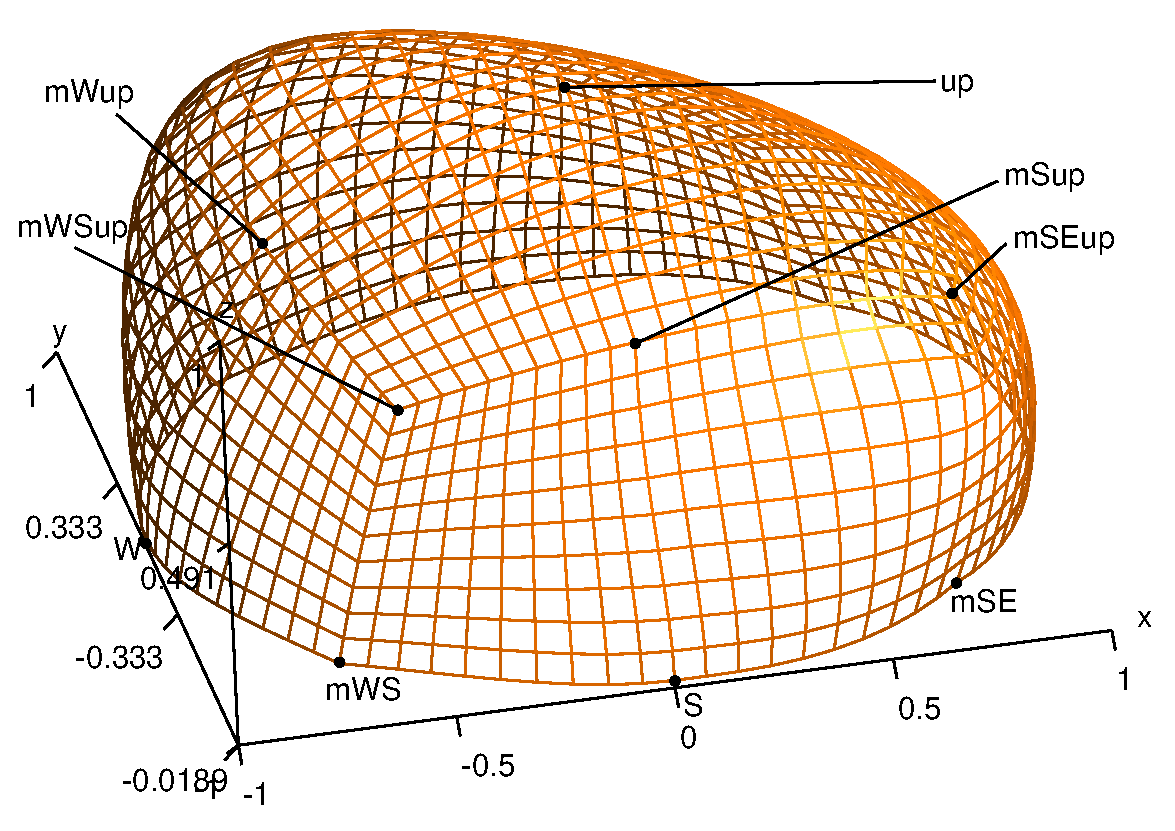
\includegraphics[width=90mm]{hemisphere-2}
  \caption{Here we have {\small\tt join}ed twelve rectangles}
  \label{\numb section 2.\numb fig 7}
\end{figure}

Note how we use a version of the {\small\tt\verm{Mesh}} constructor with
{\small\tt\textcolor{tag}{tag}::join} taking as argument a vector of {\small\tt \verm{Mesh}}es;
the same constructor is used in paragraph \ref{\numb section 9.\numb parag 2}.

Unlike in paragraph \ref{\numb section 2.\numb parag 6}, here we do not control the
exact shape of the segments {\small\tt S\_\,mSW}, {\small\tt S\_\,mSup} and so on.
They are projections of straight line segments onto our surface but since the equation
of the surface is rather complicated we do not know the exact shape of these projections.
Since points like {\small\tt mSW} and {\small\tt mSE} have been placed initially in
{\small\tt RR3} not belonging to the {\small\tt bupmy} manifold and then explicitly
{\small\tt project}ed,
there is no guarantee that they lie in the plane $ z = 0 $ (they probably don't).
We notice an angle between {\small\tt W\_\,mSW} and {\small\tt S\_\,mSW} at {\small\tt mSW}.

Paragraph \ref{\numb section 2.\numb parag 14} shows a way to control the shape of the segments
{\small\tt S\_\,mSW}, {\small\tt S\_\,mSE} and so on.

Section \ref{\numb section 3} shows other ways of meshing a surface.


          %--------%
\section{~~Exercise}\label{\numb section 2.\numb parag 8}
          %--------%

Slightly change the code in paragraph \ref{\numb section 2.\numb parag 7}
in order to obtain the mesh shown in figure \ref{\numb section 2.\numb fig 8}.
(Hint: have a look at paragraph \ref{\numb section 2.\numb parag 3}.)

\begin{figure}[ht] \centering
  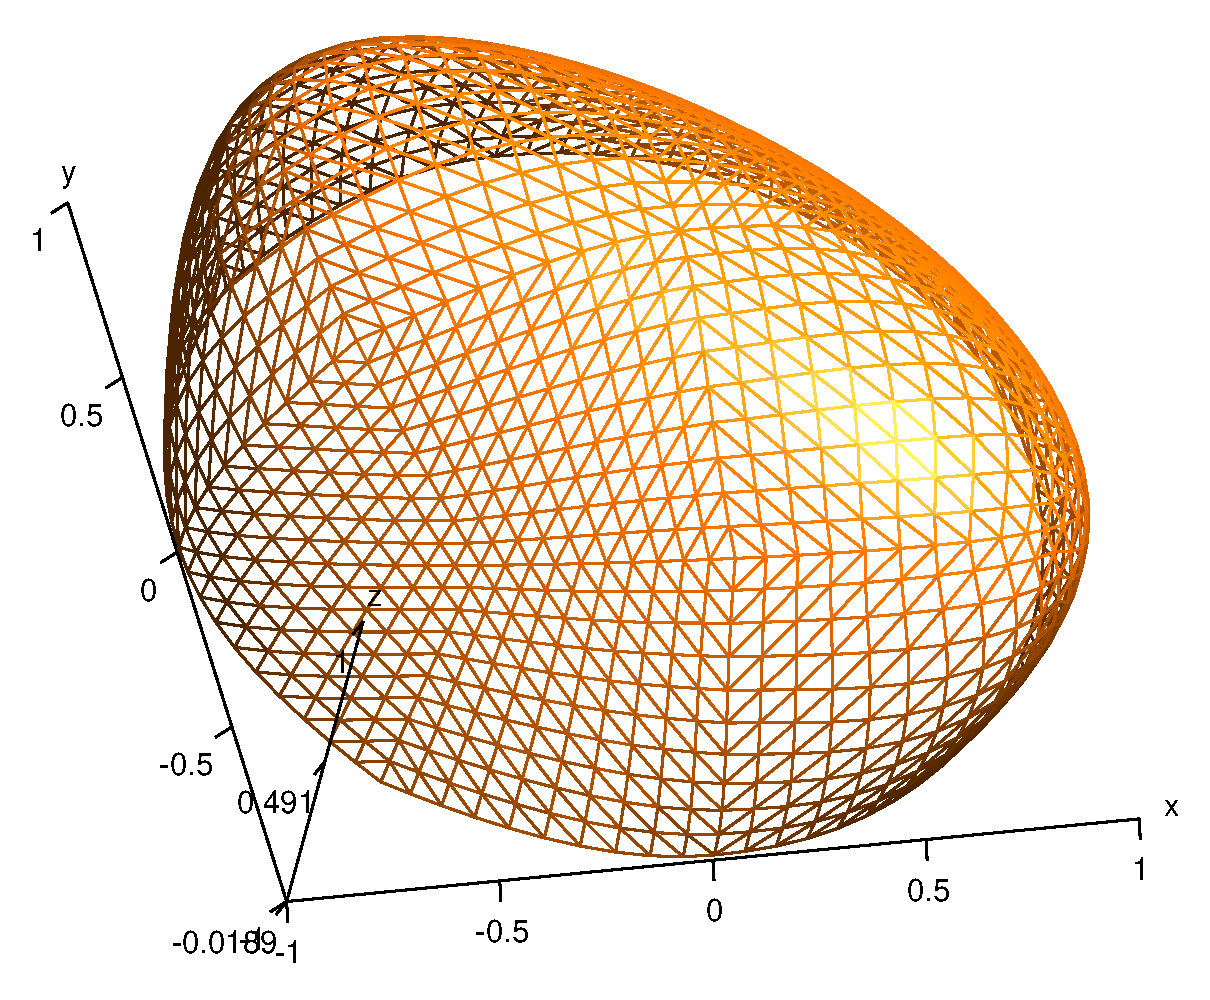
\includegraphics[width=85mm]{hemisphere-1}
  \caption{Using triangular cells}
  \label{\numb section 2.\numb fig 8}
\end{figure}


          %-----------------------------%
\section{~~Alternating between manifolds}\label{\numb section 2.\numb parag 9}
          %-----------------------------%

Let's go back to the example in paragraph \ref{\numb section 2.\numb parag 5}.
Suppose we want to mesh the whole disk, not just its boundary.
We can build the boundary of the disk just like in paragraph
\ref{\numb section 2.\numb parag 5}, by placing ourselves in the manifold {\small\tt circle}.
But if we want to subsequently mesh the interior of the disk, we must leave {\small\tt circle}
and switch back to the original {\small\tt RR2} manifold.
Method {\small\tt set\_\,as\_\,working\_\,manifold} allows us to do that.

\begin{Verbatim}[commandchars=\\\{\},formatcom=\small\tt,frame=single,
   label=parag-\ref{\numb section 2.\numb parag 9}.cpp,rulecolor=\color{coment},
   baselinestretch=0.94,framesep=2mm]
   \verm{Manifold} \azul{RR2} ( \textcolor{tag}{tag}::Euclid, \textcolor{tag}{tag}::of_dim, \laranja{2} );
   \verm{Function} \azul{xy} = RR2 .build_coordinate_system ( \textcolor{tag}{tag}::Lagrange, \textcolor{tag}{tag}::of_degree, \laranja{1} );
   \verm{Function} \azul{x} = xy [\laranja{0}], \azul{y} = xy [\laranja{1}];
   
   \verm{Manifold} \azul{circle} = RR2 .implicit ( x*x + y*y == \laranja{1.} );
   
   \verm{Cell} \azul{N} ( \textcolor{tag}{tag}::vertex );  x (N) =  \laranja{0.};  y (N) =  \laranja{1.};
   \verm{Cell} \azul{W} ( \textcolor{tag}{tag}::vertex );  x (W) = \laranja{-1.};  y (W) =  \laranja{0.};
   \verm{Cell} \azul{S} ( \textcolor{tag}{tag}::vertex );  x (S) =  \laranja{0.};  y (S) = \laranja{-1.};
   \verm{Cell} \azul{E} ( \textcolor{tag}{tag}::vertex );  x (E) =  \laranja{1.};  y (E) =  \laranja{0.};
   \verm{Mesh} \azul{NW} ( \textcolor{tag}{tag}::segment, N .reverse(), W, \textcolor{tag}{tag}::divided_in, \laranja{10} );
   \verm{Mesh} \azul{WS} ( \textcolor{tag}{tag}::segment, W .reverse(), S, \textcolor{tag}{tag}::divided_in, \laranja{10} );
   \verm{Mesh} \azul{SE} ( \textcolor{tag}{tag}::segment, S .reverse(), E, \textcolor{tag}{tag}::divided_in, \laranja{10} );
   \verm{Mesh} \azul{EN} ( \textcolor{tag}{tag}::segment, E .reverse(), N, \textcolor{tag}{tag}::divided_in, \laranja{10} );
   
   RR2 .set_as_working_manifold();
   \verm{Mesh} \azul{disk} ( \textcolor{tag}{tag}::quadrangle, NW, WS, SE, EN );
\end{Verbatim}

\begin{figure}[ht] \centering
  \psfrag{S}{\small\tt\textcolor{textindraw}{S}}
  \psfrag{N}{\small\tt\textcolor{textindraw}{N}}
  \psfrag{E}{\small\tt\textcolor{textindraw}{E}}
  \psfrag{W}{\small\tt\textcolor{textindraw}{W}}
  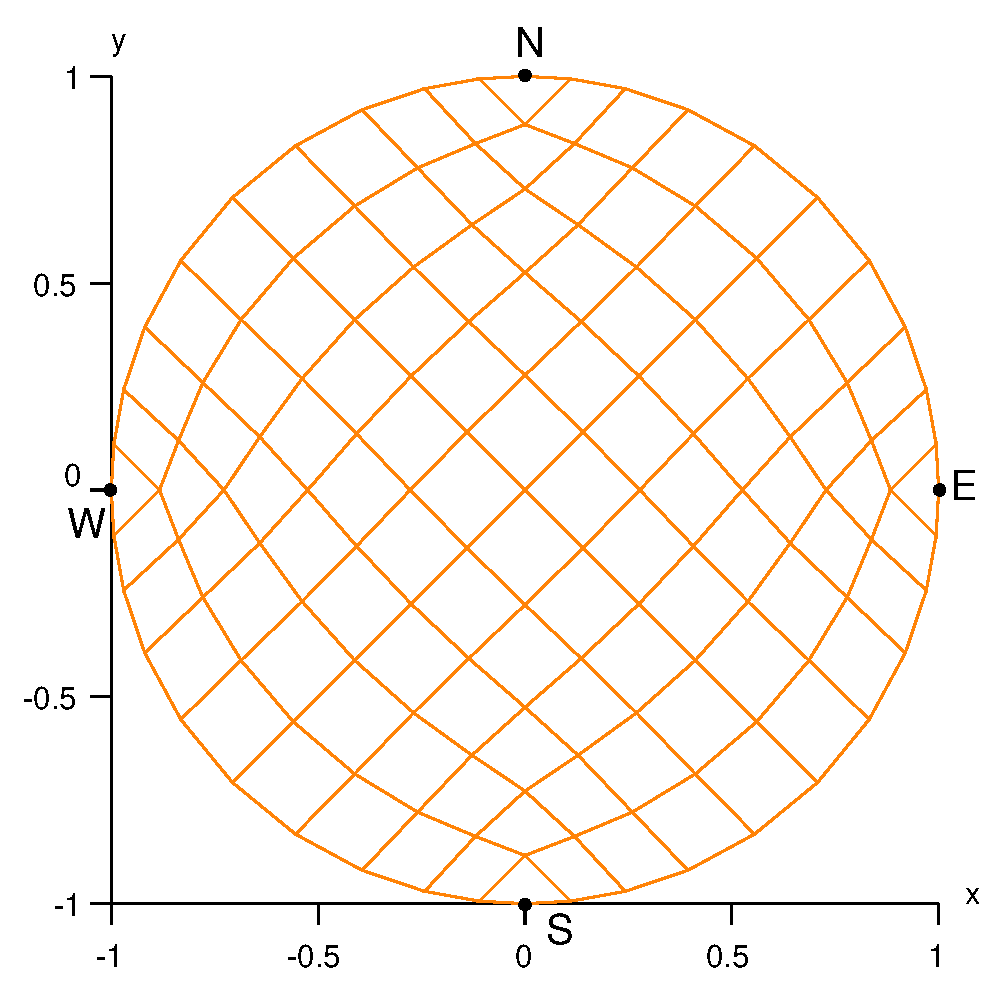
\includegraphics[width=70mm]{disk}
  \caption{A disk treated as a rectangle}
  \label{\numb section 2.\numb fig 9}
\end{figure}

The mesh (shown in figure \ref{\numb section 2.\numb fig 9}) is of poor quality;
we obtain quadrilaterals having a wide angle near {\small\tt S}, {\small\tt N}, {\small\tt E}
and {\small\tt W}.
Paragraphs \ref{\numb section 3.\numb parag 1} and \ref{\numb section 3.\numb parag 2} show
another way of meshing a disk, having its boundary as starting point.

Each time a {\small\tt\verm{Manifold}} object is created, its constructor sets it as
working manifold; this is why in many cases we don't need to know about method
{\small\tt set\_\,as\_\,working\_\,manifold}.
We need it, however, in cases like the one presented here.


          %--------%
\section{~~Exercise}\label{\numb section 2.\numb parag 10}
          %--------%

Mesh half of a disk by joining three triangular meshes
(see figure \ref{\numb section 2.\numb fig 10}).
Mesh the entire disk by joining six triangular meshes.

\begin{figure}[ht] \centering
  \psfrag{S}{\small\tt\textcolor{textindraw}{S}}
  \psfrag{N}{\small\tt\textcolor{textindraw}{N}}
  \psfrag{E}{\small\tt\textcolor{textindraw}{E}}
  \psfrag{W}{\small\tt\textcolor{textindraw}{W}}
  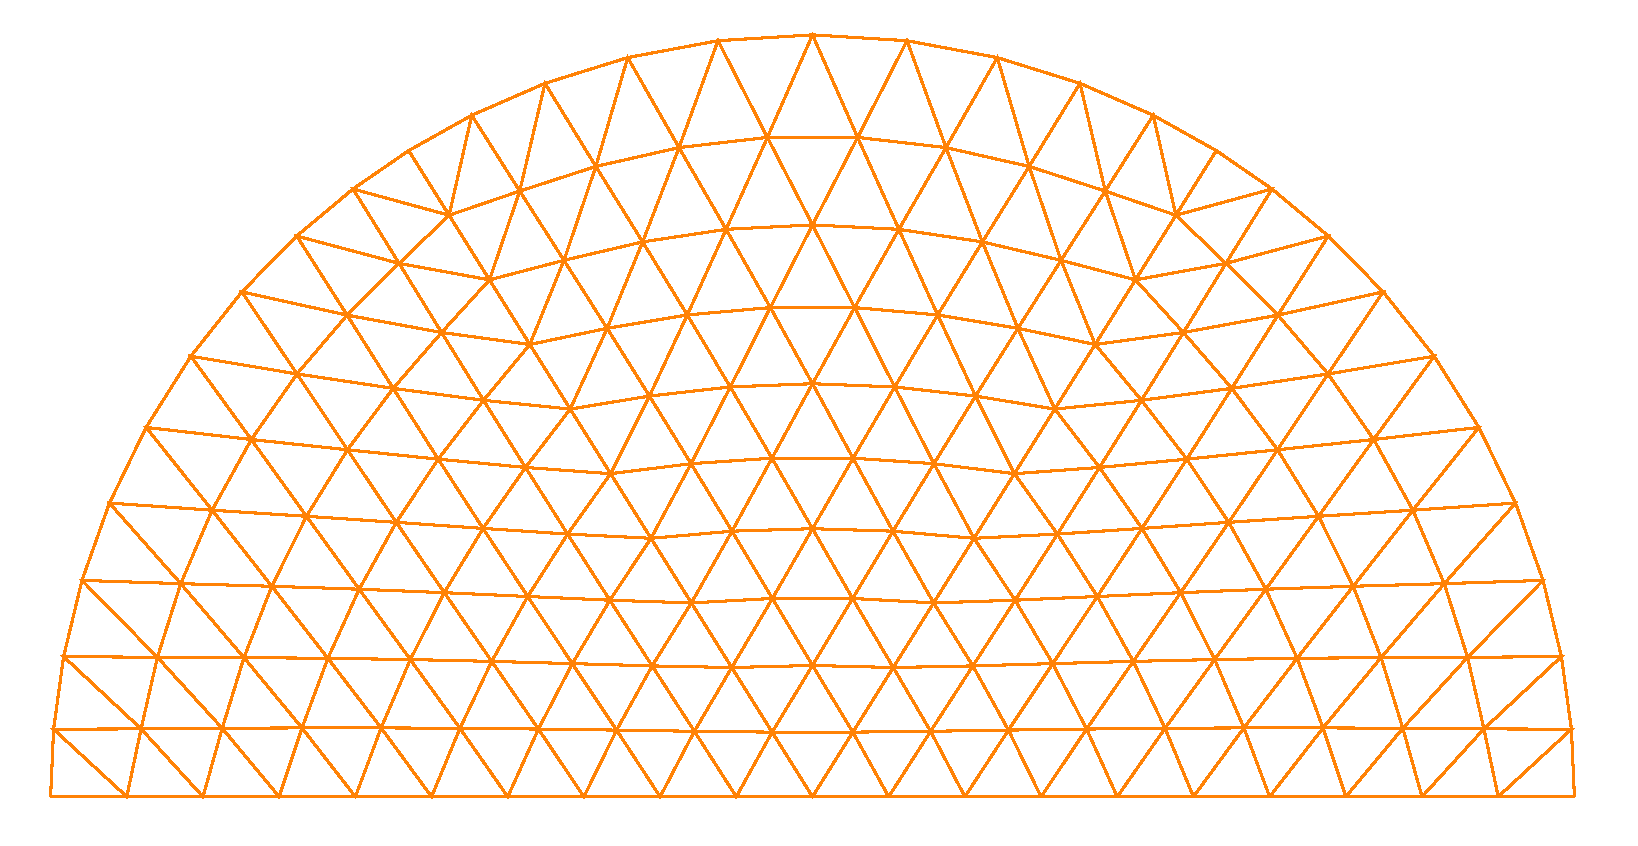
\includegraphics[width=95mm]{half-disk}
  \caption{Half disk}
  \label{\numb section 2.\numb fig 10}
\end{figure}


          %------------------------------------%
\section{~~Alternating between manifolds, again}\label{\numb section 2.\numb parag 11}
          %------------------------------------%


Here is an example similar to the one in paragraph \ref{\numb section 2.\numb parag 9},
this time with four arcs of hiperbola.

\begin{figure}[ht] \centering
  \psfrag{S}{\small\tt\textcolor{textindraw}{S}}
  \psfrag{N}{\small\tt\textcolor{textindraw}{N}}
  \psfrag{E}{\small\tt\textcolor{textindraw}{E}}
  \psfrag{W}{\small\tt\textcolor{textindraw}{W}}
  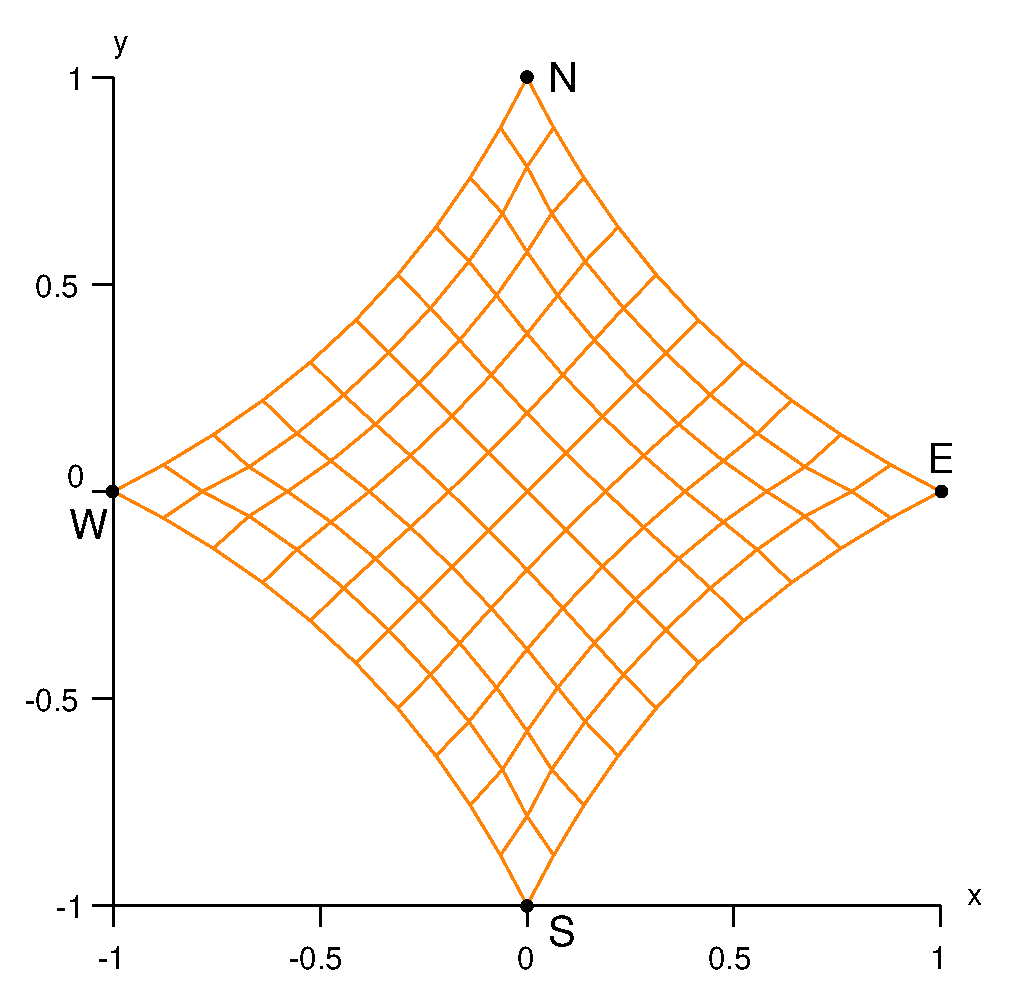
\includegraphics[width=80mm]{diamond}
  \caption{A diamond shape}
  \label{\numb section 2.\numb fig 11}
\end{figure}

\begin{Verbatim}[commandchars=\\\{\},formatcom=\small\tt,frame=single,
   label=parag-\ref{\numb section 2.\numb parag 11}.cpp,rulecolor=\color{coment},
   baselinestretch=0.94,framesep=2mm]
   \verm{Manifold} \azul{RR2} ( \textcolor{tag}{tag}::Euclid, \textcolor{tag}{tag}::of_dim, \laranja{2} );
   \verm{Function} \azul{xy} = RR2 .build_coordinate_system ( \textcolor{tag}{tag}::Lagrange, \textcolor{tag}{tag}::of_degree, \laranja{1} );
   \verm{Function} \azul{x} = xy [\laranja{0}], \azul{y} = xy [\laranja{1}];
   \verm{Cell} \azul{N} ( \textcolor{tag}{tag}::vertex );  x (N) =  \laranja{0.};  y (N) =  \laranja{1.};
   \verm{Cell} \azul{W} ( \textcolor{tag}{tag}::vertex );  x (W) = \laranja{-1.};  y (W) =  \laranja{0.};
   \verm{Cell} \azul{S} ( \textcolor{tag}{tag}::vertex );  x (S) =  \laranja{0.};  y (S) = \laranja{-1.};
   \verm{Cell} \azul{E} ( \textcolor{tag}{tag}::vertex );  x (E) =  \laranja{1.};  y (E) =  \laranja{0.};
   \verm{Manifold} \azul{first_arc}  = RR2 .implicit ( x*y + x - y == \laranja{-1.} );
   \verm{Mesh} \azul{NW} ( \textcolor{tag}{tag}::segment, N .reverse(), W, \textcolor{tag}{tag}::divided_in, \laranja{10} );
   \verm{Manifold} \azul{second_arc} = RR2 .implicit ( x*y - x - y ==  \laranja{1.} );
   \verm{Mesh} \azul{WS} ( \textcolor{tag}{tag}::segment, W .reverse(), S, \textcolor{tag}{tag}::divided_in, \laranja{10} );
   \verm{Manifold} \azul{third_arc}  = RR2 .implicit ( x*y - x + y == \laranja{-1.} );
   \verm{Mesh} \azul{SE} ( \textcolor{tag}{tag}::segment, S .reverse(), E, \textcolor{tag}{tag}::divided_in, \laranja{10} );
   \verm{Manifold} \azul{fourth_arc} = RR2 .implicit ( x*y + x + y ==  \laranja{1.} );
   \verm{Mesh} \azul{EN} ( \textcolor{tag}{tag}::segment, E .reverse(), N, \textcolor{tag}{tag}::divided_in, \laranja{10} );
   
   RR2 .set_as_working_manifold();
   \verm{Mesh} \azul{diamond} ( \textcolor{tag}{tag}::quadrangle, NW, WS, SE, EN );
\end{Verbatim}

Paragraph \ref{\numb section 3.\numb parag 17} shows another way of meshing the same domain.
\vfil\eject


          %----------------%
\section{~~An organic shape}\label{\numb section 2.\numb parag 12}
          %----------------%

This paragraph describes a surface meant to mimic the shape of a physalis fruit.

%\begin{figure}[h!]\centering
%  
\includegraphics[width=85mm]{empty}
%  \caption{Dry physalis, with fruit inside}\label{\numb section 2.\numb fig 12}
%\end{figure}

\begin{figure}[ht]\centering
%\vskip -3mm
\if\production 1
\centerline{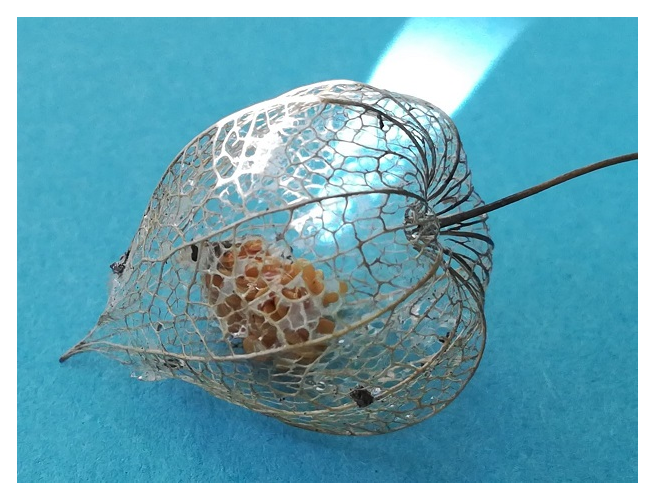
\includegraphics[width=65mm]{dry-physalis}}
\else
\psfrag{photo}{[photo of a physalis]}
\centerline{
\includegraphics[width=75mm]{fake-physalis}}
\fi
  \caption{Dry physalis, with fruit inside}\label{\numb section 2.\numb fig 12}
\end{figure}
%\vfil\eject

We begin by defining a revolution surface in $ \mathbb{R}^3 $ :

\begin{Verbatim}[commandchars=\\\{\},formatcom=\small\tt,frame=single,
   label=parag-\ref{\numb section 2.\numb parag 12}.cpp,rulecolor=\color{coment},
   baselinestretch=0.94,framesep=2mm]
   \verm{Function} \azul{r2} = x*x + y*y + z*z;
   const double \azul{pi} = \laranja{3.1415926536};
   \verm{Manifold} \azul{apple} = RR3 .implicit ( \verm{power}(r2,\laranja{0.5}) * \verm{sin}(r2-pi/\laranja{6.}) == z );
\end{Verbatim}

This surface has the shape shown in figure \ref{\numb section 2.\numb fig 13},
which does not resemble a physalis fruit.

\begin{figure}[ht] \centering
  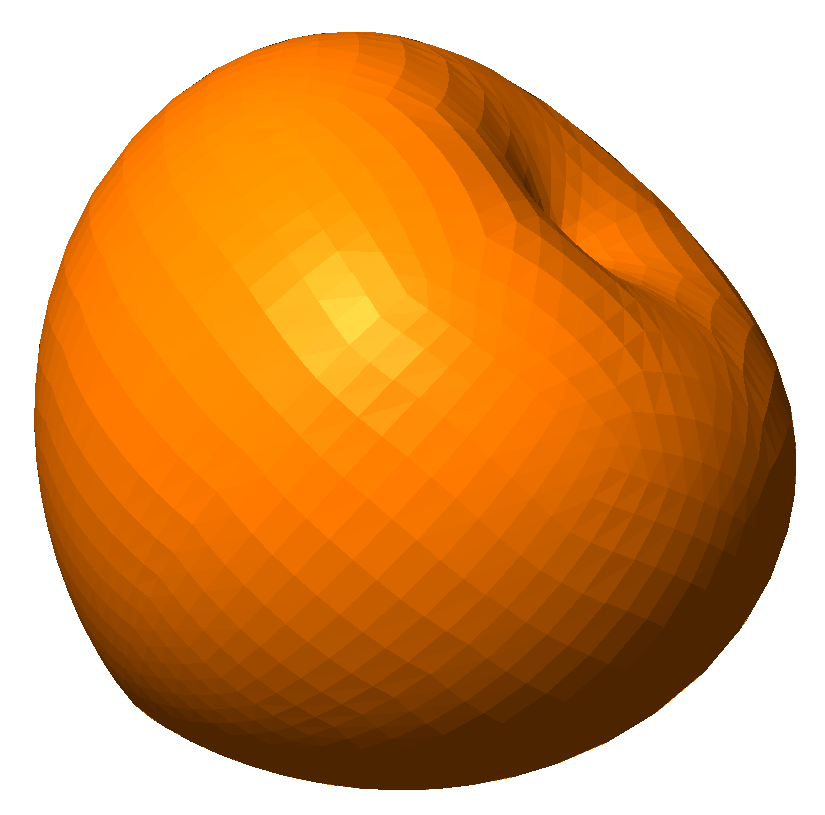
\includegraphics[width=55mm]{fisalis-manif}
  \caption{A compact manifold resembling an apple}
  \label{\numb section 2.\numb fig 13}
\end{figure}

Instead of meshing the {\small\tt apple} surface, we just build eight curves immersed in it
(each curve joins {\small\tt A} to {\small\tt D} and is made of three shorter curves) :

\begin{Verbatim}[commandchars=\\\{\},formatcom=\small\tt,frame=single,
   label=parag-\ref{\numb section 2.\numb parag 12}.cpp,rulecolor=\color{coment},
   baselinestretch=0.94,framesep=2mm]
   \verm{Cell} \azul{A} ( \textcolor{tag}{tag}::vertex );  x (A) = \laranja{0.};  y (A) = \laranja{0.};  z (A) = std::sqrt ( \laranja{2.}*pi/\laranja{3.} );
   \verm{Cell} \azul{B1} ( \textcolor{tag}{tag}::vertex );  x (B1) = \laranja{1.};  y (B1) = \laranja{0.};  z (B1) = \laranja{1.};
   \verm{Cell} \azul{C1} ( \textcolor{tag}{tag}::vertex );  x (C1) = \laranja{1.};  y (C1) = \laranja{0.};  z (C1) = \laranja{0.};
   apple .project (B1);  apple .project (C1);
   \verm{Cell} \azul{D} ( \textcolor{tag}{tag}::vertex );  x (D) = \laranja{0.};  y (D) = \laranja{0.};  z (D) = \laranja{0.};
   \verm{Mesh} \azul{AB1} ( \textcolor{tag}{tag}::segment, A .reverse(), B1, \textcolor{tag}{tag}::divided_in, \laranja{10} );
   \verm{Mesh} \azul{B1C1} ( \textcolor{tag}{tag}::segment, B1 .reverse(), C1, \textcolor{tag}{tag}::divided_in, \laranja{10} );
   \verm{Mesh} \azul{C1D} ( \textcolor{tag}{tag}::segment, C1 .reverse(), D, \textcolor{tag}{tag}::divided_in, \laranja{10} );
   \cinza{// and so on ...}
\end{Verbatim}

Then we switch back to {\small\tt RR3} (thus leaving the {\small\tt apple} manifold) and build
transversal segments, as well as triangular and quadrangular patches :

\begin{Verbatim}[commandchars=\\\{\},formatcom=\small\tt,frame=single,
   label=parag-\ref{\numb section 2.\numb parag 12}.cpp,rulecolor=\color{coment},
   baselinestretch=0.94,framesep=2mm]
   RR3 .set_as_working_manifold();
   \verm{Mesh} \azul{B1B2} ( \textcolor{tag}{tag}::segment, B1 .reverse(), B2, \textcolor{tag}{tag}::divided_in, \laranja{10} );
   \verm{Mesh} \azul{B2B3} ( \textcolor{tag}{tag}::segment, B2 .reverse(), B3, \textcolor{tag}{tag}::divided_in, \laranja{10} );
   \cinza{// and many other segments ...}
   \verm{Mesh} \azul{AB1B2} ( \textcolor{tag}{tag}::triangle, AB1, B1B2, AB2 .reverse() );
   \verm{Mesh} \azul{AB2B3} ( \textcolor{tag}{tag}::triangle, AB2, B2B3, AB3 .reverse() );
   \cinza{// and other triangular patches ...}
   \verm{Mesh} \azul{B1C1C2B2} ( \textcolor{tag}{tag}::quadrangle, B1C1, C1C2, B2C2 .reverse(), B1B2 .reverse(),
                   \textcolor{tag}{tag}::with_triangles                                           );
   \verm{Mesh} \azul{B2C2C3B3} ( \textcolor{tag}{tag}::quadrangle, B2C2, C2C3, B3C3 .reverse(), B2B3 .reverse(),
                   \textcolor{tag}{tag}::with_triangles                                           );
   \cinza{// and other quadrangular patches ...}   
\end{Verbatim}

We then join all patches :
\begin{Verbatim}[commandchars=\\\{\},formatcom=\small\tt,frame=single,
   label=parag-\ref{\numb section 2.\numb parag 12}.cpp,rulecolor=\color{coment},
   baselinestretch=0.94,framesep=2mm]
   \verm{Mesh} \azul{sect1} ( \textcolor{tag}{tag}::join, AB1B2, B1C1C2B2, C1DC2 );
   \verm{Mesh} \azul{sect2} ( \textcolor{tag}{tag}::join, AB2B3, B2C2C3B3, C2DC3 );
   \cinza{// more sectors ...}
   std::vector < \verm{Mesh} > lm \{ sect1, sect2, sect3, sect4, sect5, sect6, sect7, sect8 \};
   \verm{Mesh} \azul{fisalis} ( \textcolor{tag}{tag}::join, lm ); 
\end{Verbatim}

\begin{figure}[ht] \centering
  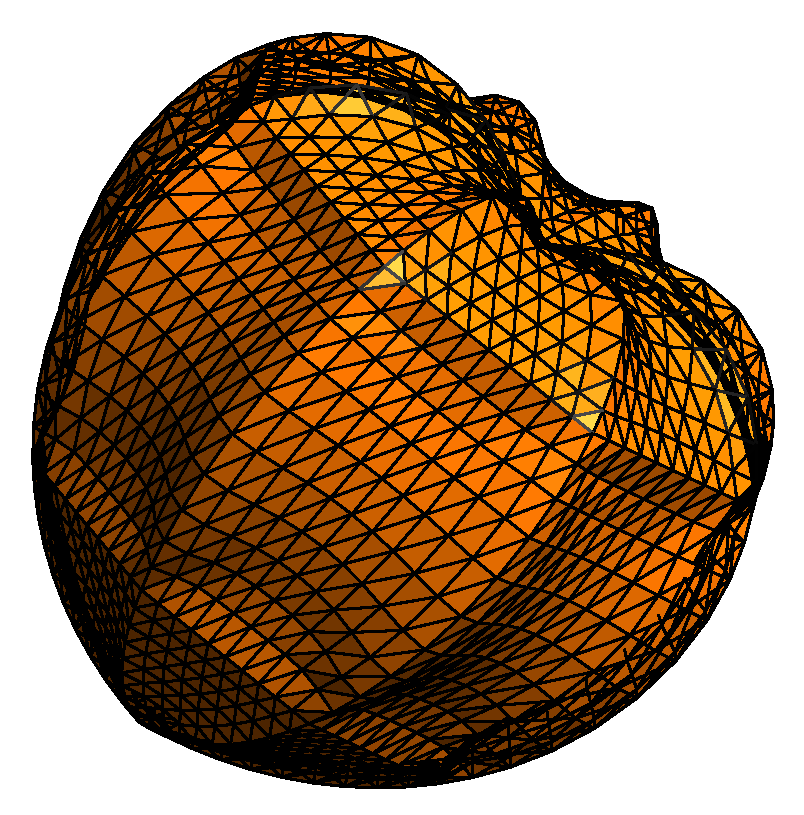
\includegraphics[width=45mm]{fisalis-round}
  \caption{Not yet a physalis}
  \label{\numb section 2.\numb fig 14}
\end{figure}

This shape is still not satisfactory, so we apply a deformation in $ \mathbb{R}^3 $ in order to
get a sharper tip.
The {\small\tt apple} manifold is no longer relevant.

\begin{Verbatim}[commandchars=\\\{\},formatcom=\small\tt,frame=single,
   label=parag-\ref{\numb section 2.\numb parag 12}.cpp,rulecolor=\color{coment},
   baselinestretch=0.94,framesep=2mm]
   \verm{Mesh}::Iterator \azul{it} = fisalis .iterator ( \textcolor{tag}{tag}::over_vertices );
   for ( it .reset(); it .in_range(); it++ )
   \{  \verm{Cell} \azul{P} = *it;
      x(P) *= \laranja{0.8};  y(P) *= \laranja{0.8};
      if ( z(P) > \laranja{1.3} )
      \{  x(P) = x(P) / ( \laranja{1.} + \laranja{300.} * std::pow ( z(P) - \laranja{1.3}, \laranja{3.} ) );
         y(P) = y(P) / ( \laranja{1.} + \laranja{300.} * std::pow ( z(P) - \laranja{1.3}, \laranja{3.} ) );
         z(P) = z(P) * ( \laranja{1.} + \laranja{10.} * ( z(P) - \laranja{1.3} ) * ( z(P) - \laranja{1.3} ) );  \}
      if ( z(P) > \laranja{0.} ) z(P) *= \laranja{0.8};                                        \}
\end{Verbatim}

Paragraph \ref{\numb section 9.\numb parag 3} explains the notion of an iterator over cells.

We add a sequence of baricenter operations for smoothening the shape.
Note that each baricenter operation is relative to a sector and it applies only to inner
vertices, so the boundary of the sector is not changed.
Thus, the eight rims defined in the beginning are kept unchanged.

\begin{Verbatim}[commandchars=\\\{\},formatcom=\small\tt,frame=single,
   label=parag-\ref{\numb section 2.\numb parag 12}.cpp,rulecolor=\color{coment},
   baselinestretch=0.94,framesep=2mm]
   std::vector < \verm{Mesh} > ::iterator \azul{it1};
   for ( it1 = lm .begin(); it1 != lm .end(); it1++ )
   \{  \verm{Mesh} \azul{sect} = *it1;
      \verm{Mesh}::Iterator \azul{it2} = sect .iterator ( \textcolor{tag}{tag}::over_vertices );
      for ( int \azul{i} = \laranja{1}; i < \laranja{20}; i++ )
      for ( it2 .reset(); it2 .in_range(); it2++ )
      \{  \verm{Cell} \azul{ver} = *it2;
         if ( ver .is_inner_to ( sect ) ) sect .baricenter ( ver );  \}  \}
\end{Verbatim}

And we are happy with the final result, shown in figure \ref{\numb section 2.\numb fig 15}.

\begin{figure}[ht] \centering
  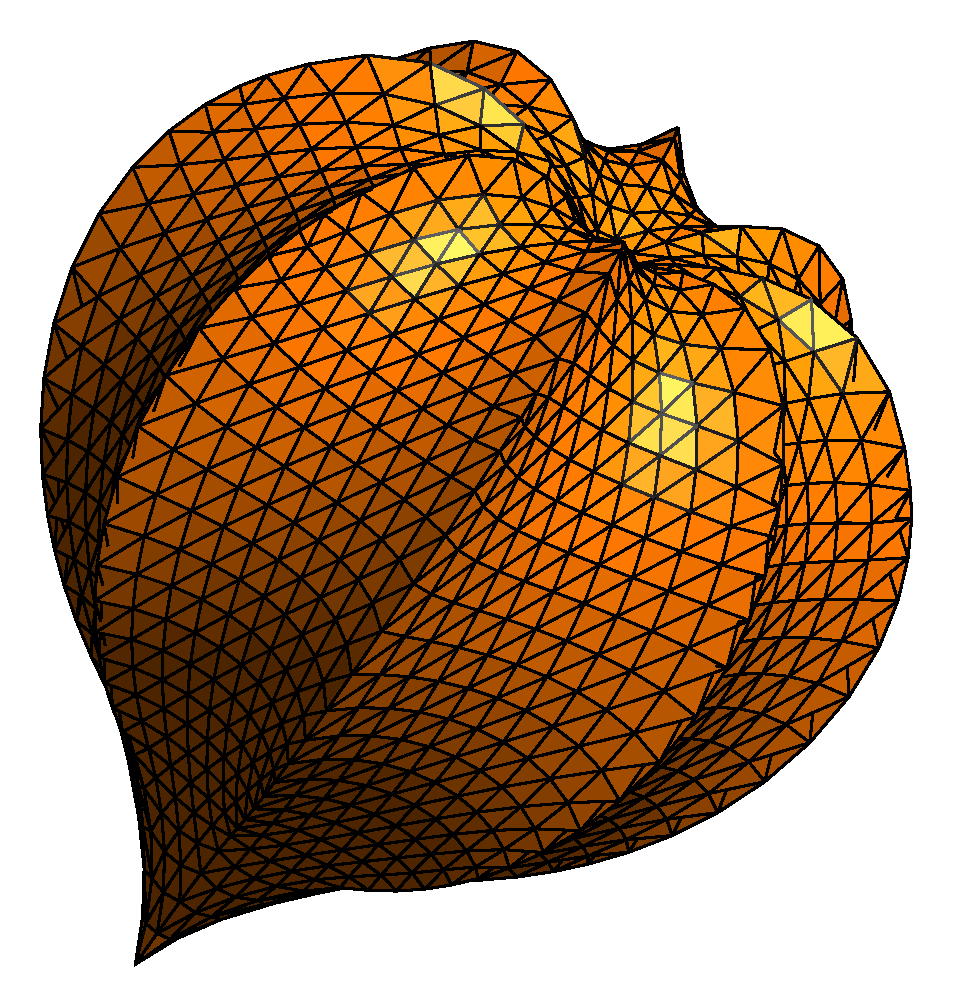
\includegraphics[width=60mm]{fisalis}
  \caption{Meshing a chinese lantern}
  \label{\numb section 2.\numb fig 15}
\end{figure}

An animation related to this example is available at\hfil\break
{\small\tt http://manifem.rd.ciencias.ulisboa.pt/apple-to-physalis.gif}


          %-----------------------------------%
\section{~~A manifold defined by two equations}\label{\numb section 2.\numb parag 13}
          %-----------------------------------%

We can define a one-dimensional submanifold of $ \mathbb{R}^3 $ by two implicit equations :
\medskip

\begin{figure}[ht] \centering
  \psfrag{S}{\small\tt\textcolor{textindraw}{S}}
  \psfrag{N}{\small\tt\textcolor{textindraw}{N}}
  \psfrag{E}{\small\tt\textcolor{textindraw}{E}}
  \psfrag{W}{\small\tt\textcolor{textindraw}{W}}
  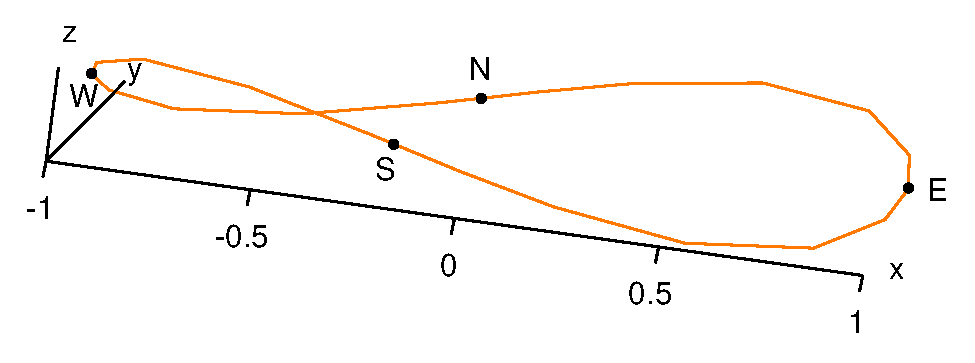
\includegraphics[width=75mm]{circle-3d}
  \caption{One-dimensional mesh in $ {\mathbb R}^3 $}
  \label{\numb section 2.\numb fig 16}
\end{figure}

\begin{Verbatim}[commandchars=\\\{\},formatcom=\small\tt,frame=single,
   label=parag-\ref{\numb section 2.\numb parag 13}.cpp,rulecolor=\color{coment},
   baselinestretch=0.94,framesep=2mm]
   \verm{Manifold} \azul{RR3} ( \textcolor{tag}{tag}::Euclid, \textcolor{tag}{tag}::of_dim, \laranja{3} );
   \verm{Function} \azul{xyz} = RR3 .build_coordinate_system ( \textcolor{tag}{tag}::Lagrange, \textcolor{tag}{tag}::of_degree, \laranja{1} );
   \verm{Function} \azul{x} = xyz [\laranja{0}], \azul{y} = xyz [\laranja{1}], \azul{z} = xyz [\laranja{2}];
   \verm{Manifold} \azul{circle_manifold} = RR3 .implicit ( x*x + y*y == \laranja{1.}, x*y == \laranja{4.}*z );

   \verm{Cell} \azul{S} ( \textcolor{tag}{tag}::vertex );  x (S) =  \laranja{0.};  y (S) = \laranja{-1.};  z (S) = \laranja{0.};
   \verm{Cell} \azul{E} ( \textcolor{tag}{tag}::vertex );  x (E) =  \laranja{1.};  y (E) =  \laranja{0.};  z (E) = \laranja{0.};
   \verm{Cell} \azul{N} ( \textcolor{tag}{tag}::vertex );  x (N) =  \laranja{0.};  y (N) =  \laranja{1.};  z (N) = \laranja{0.};
   \verm{Cell} \azul{W} ( \textcolor{tag}{tag}::vertex );  x (W) = \laranja{-1.};  y (W) =  \laranja{0.};  z (W) = \laranja{0.};
   \cinza{// these four points already belong to 'circle_manifold', no projection needed}

   \verm{Mesh} \azul{SE} ( \textcolor{tag}{tag}::segment, S .reverse(), E, \textcolor{tag}{tag}::divided_in, \laranja{5} );
   \verm{Mesh} \azul{EN} ( \textcolor{tag}{tag}::segment, E .reverse(), N, \textcolor{tag}{tag}::divided_in, \laranja{5} );
   \verm{Mesh} \azul{NW} ( \textcolor{tag}{tag}::segment, N .reverse(), W, \textcolor{tag}{tag}::divided_in, \laranja{5} );
   \verm{Mesh} \azul{WS} ( \textcolor{tag}{tag}::segment, W .reverse(), S, \textcolor{tag}{tag}::divided_in, \laranja{5} );

   \verm{Mesh} \azul{circle} ( \textcolor{tag}{tag}::join, SE, EN, NW, WS );
\end{Verbatim}

Paragraph \ref{\numb section 3.\numb parag 4} shows another way of meshing the same loop.


          %------------------------------%
\section{~~A submanifold of a submanifold}\label{\numb section 2.\numb parag 14}
          %------------------------------%

An implicit manifold has submanifolds.
For instance, we can improve the look of the ``bumpy hemisphere'' in paragraph
\ref{\numb section 2.\numb parag 7} by building its base (a circle-like closed curve)
inside a one-dimensional manifold.
For the rest of the surface, we switch back to the two-dimensional manifold {\small\tt nut} :
\medskip

\begin{figure}[ht] \centering
  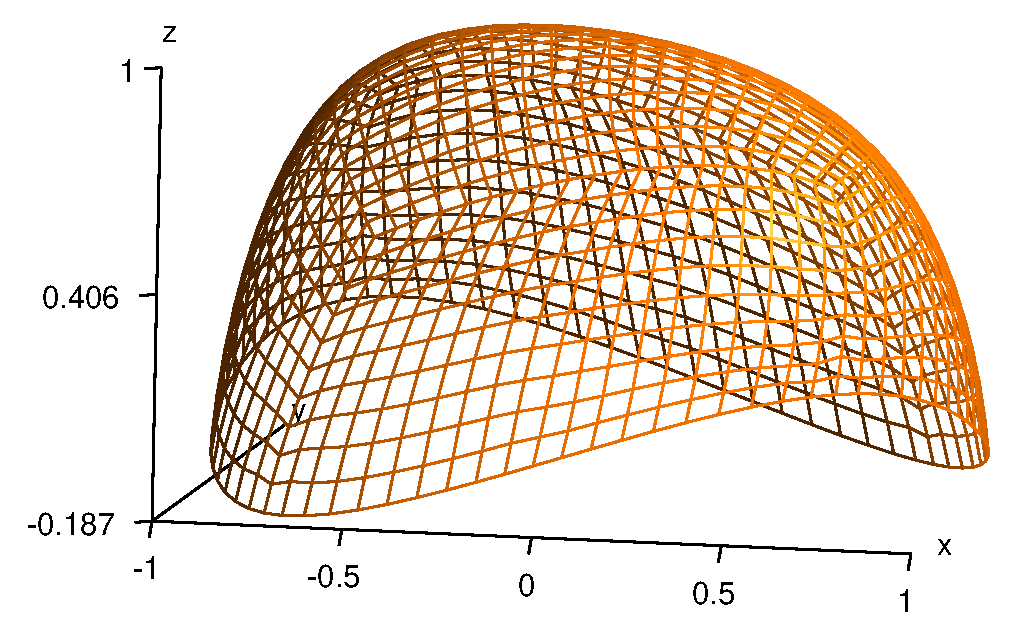
\includegraphics[width=100mm]{bumpy}
  \caption{A shell}
  \label{\numb section 2.\numb fig 17}
\end{figure}

\begin{Verbatim}[commandchars=\\\{\},formatcom=\small\tt,frame=single,
   label=parag-\ref{\numb section 2.\numb parag 14}.cpp,rulecolor=\color{coment},
   baselinestretch=0.94,framesep=2mm]
   \verm{Manifold} \azul{nut} = RR3 .implicit ( x*x + y*y + z*z + \laranja{1.5}*x*y*z == \laranja{1.} );
   int \azul{n} = \laranja{10};

   \cinza{// first build the base (a closed curve)}
   \verm{Manifold} \azul{base} = nut .implicit ( x*x + \laranja{3.}*z == \laranja{0.} );

   \verm{Cell} \azul{S} ( \textcolor{tag}{tag}::vertex );  x (S) =  \laranja{0.};  y (S) = \laranja{-1.};  z (S) =  \laranja{0.};
   \verm{Cell} \azul{E} ( \textcolor{tag}{tag}::vertex );  x (E) =  \laranja{1.};  y (E) =  \laranja{0.};  z (E) =  \laranja{0.};
   \verm{Cell} \azul{N} ( \textcolor{tag}{tag}::vertex );  x (N) =  \laranja{0.};  y (N) =  \laranja{1.};  z (N) =  \laranja{0.};
   \verm{Cell} \azul{W} ( \textcolor{tag}{tag}::vertex );  x (W) = \laranja{-1.};  y (W) =  \laranja{0.};  z (W) =  \laranja{0.};
   \cinza{// no need to project S and N, they are already on 'base'}
   base .project (E);  base .project (W);
   \verm{Cell} \azul{mSW} ( \textcolor{tag}{tag}::vertex );  x (mSW) = \laranja{-1.};  y (mSW) = \laranja{-1.};  z (mSW) = \laranja{0.};
   base .project ( mSW );  \cinza{// midway between S and W}
   \verm{Cell} \azul{mSE} ( \textcolor{tag}{tag}::vertex );  x (mSE) =  \laranja{1.};  y (mSE) = \laranja{-1.};  z (mSW) = \laranja{0.};
   base .project ( mSE );  \cinza{// midway between S and E}
   \cinza{// define similarly mNE and mNW}

   \cinza{// now build eight segments, forming the base}
   \verm{Mesh} \azul{S_mSW} ( \textcolor{tag}{tag}::segment, S .reverse(), mSW, \textcolor{tag}{tag}::divided_in, n );
   \verm{Mesh} \azul{S_mSE} ( \textcolor{tag}{tag}::segment, S .reverse(), mSE, \textcolor{tag}{tag}::divided_in, n );
   \verm{Mesh} \azul{E_mSE} ( \textcolor{tag}{tag}::segment, E .reverse(), mSE, \textcolor{tag}{tag}::divided_in, n );
   \verm{Mesh} \azul{E_mNE} ( \textcolor{tag}{tag}::segment, E .reverse(), mNE, \textcolor{tag}{tag}::divided_in, n );
   \verm{Mesh} \azul{N_mNE} ( \textcolor{tag}{tag}::segment, N .reverse(), mNE, \textcolor{tag}{tag}::divided_in, n );
   \verm{Mesh} \azul{N_mNW} ( \textcolor{tag}{tag}::segment, N .reverse(), mNW, \textcolor{tag}{tag}::divided_in, n );
   \verm{Mesh} \azul{W_mSW} ( \textcolor{tag}{tag}::segment, W .reverse(), mSW, \textcolor{tag}{tag}::divided_in, n );
   \verm{Mesh} \azul{W_mNW} ( \textcolor{tag}{tag}::segment, W .reverse(), mNW, \textcolor{tag}{tag}::divided_in, n );

   \cinza{// we are done with the base, now switch back to 'nut'}
   nut .set_as_working_manifold();
   \cinza{// more points :}
   \verm{Cell} \azul{up} ( \textcolor{tag}{tag}::vertex );  x (up) = \laranja{0.};  y (up) = \laranja{0.};  z (up) = \laranja{1.};
   \cinza{// no need to project 'up', it is already on 'nut'}
   \verm{Cell} \azul{mSup}  ( \textcolor{tag}{tag}::vertex );  x (mSup) = \laranja{0.};  y (mSup) = \laranja{-1.};  z (mSup) = \laranja{1.};
   nut .project ( mSup );  \cinza{// midway between S and up}
   \verm{Cell} \azul{mSWup} ( \textcolor{tag}{tag}::vertex );  x (mSWup) = \laranja{-1.};  y (mSWup) = \laranja{-1.};  z (mSWup) = \laranja{1.};
   nut .project ( mSWup );  \cinza{// somewhere between S, W and up}
   \cinza{// ... and so forth ...}

   \cinza{// more segments :}
   \verm{Mesh} \azul{W_mWup} ( \textcolor{tag}{tag}::segment, W .reverse(), mWup, \textcolor{tag}{tag}::divided_in, n );
   \verm{Mesh} \azul{mSW_mSWup} ( \textcolor{tag}{tag}::segment, mSW .reverse(), mSWup, \textcolor{tag}{tag}::divided_in, n );
   \verm{Mesh} \azul{mWup_mSWup} ( \textcolor{tag}{tag}::segment, mWup .reverse(), mSWup, \textcolor{tag}{tag}::divided_in, n );
   \cinza{// ... and so forth ...}
\end{Verbatim}

If we wanted a flat base, we could have defined

\begin{Verbatim}[commandchars=\\\{\},formatcom=\small\tt,baselinestretch=0.94]
   \verm{Manifold} \azul{base} = nut .implicit ( z == \laranja{0.} );
\end{Verbatim}

Paragraph \ref{\numb section 3.\numb parag 9} shows a way to mesh the same surface using
fewer lines of code.


          %-------------------------------%
\section{~~Parametric manifolds -- a curve}\label{\numb section 2.\numb parag 15}
          %-------------------------------%

Paragraphs \ref{\numb section 2.\numb parag 4} -- \ref{\numb section 2.\numb parag 14} describe
manifolds defined through implicit equations, that is, level sets in $ \mathbb{R}^2 $ or
$ \mathbb{R}^3 $.
Another way of defining a submanifold is through a parametrization.
Below is an example.

\begin{Verbatim}[commandchars=\\\{\},formatcom=\small\tt,frame=single,
   label=parag-\ref{\numb section 2.\numb parag 15}.cpp,rulecolor=\color{coment},
   baselinestretch=0.94,framesep=2mm]
   \cinza{// at the beginning, we define 'spiral' as a straight line}
   \verm{Manifold} \azul{spiral} ( \textcolor{tag}{tag}::Euclid, \textcolor{tag}{tag}::of_dim, \laranja{1} );
   \verm{Function} \azul{t} = spiral .build_coordinate_system ( \textcolor{tag}{tag}::Lagrange, \textcolor{tag}{tag}::of_degree, 1 );

   \cinza{// now build 'arc_of_spiral' merely as a segment from pi/2 to 5 pi}
   const double \azul{pi} = \laranja{3.1415926536};
   \verm{Cell} \azul{A} ( \textcolor{tag}{tag}::vertex );  t (A) = pi/\laranja{2.};
   \verm{Cell} \azul{B} ( \textcolor{tag}{tag}::vertex );  t (B) = \laranja{5.}*pi;

   \verm{Mesh} \azul{arc_of_spiral} ( \textcolor{tag}{tag}::segment, A .reverse(), B, \textcolor{tag}{tag}::divided_in, \laranja{30} );
   \cinza{// not very interesting for now}
   \cinza{// but now define functions x and y as expressions of t :}
   \verm{Function} \azul{x} = t * \verm{cos}(t), \azul{y} = t * \verm{sin}(t);
   \cinza{// and declare them to be the new coordinates}
   \verm{Manifold} \azul{RR2} ( tag::Euclid, \textcolor{tag}{tag}::of_dimension, \laranja{2} );
   RR2 .set_coordinates ( x && y );
   \cinza{// in future statements (e.g. for graphical representation)}
   \cinza{// x and y will be used, not t :}
   arc_of_spiral .draw_ps (\verde{"spiral.eps"});
\end{Verbatim}

\begin{figure}[ht] \centering
  \psfrag{A}{\small\tt\textcolor{textindraw}{A}}
  \psfrag{B}{\small\tt\textcolor{textindraw}{B}}
  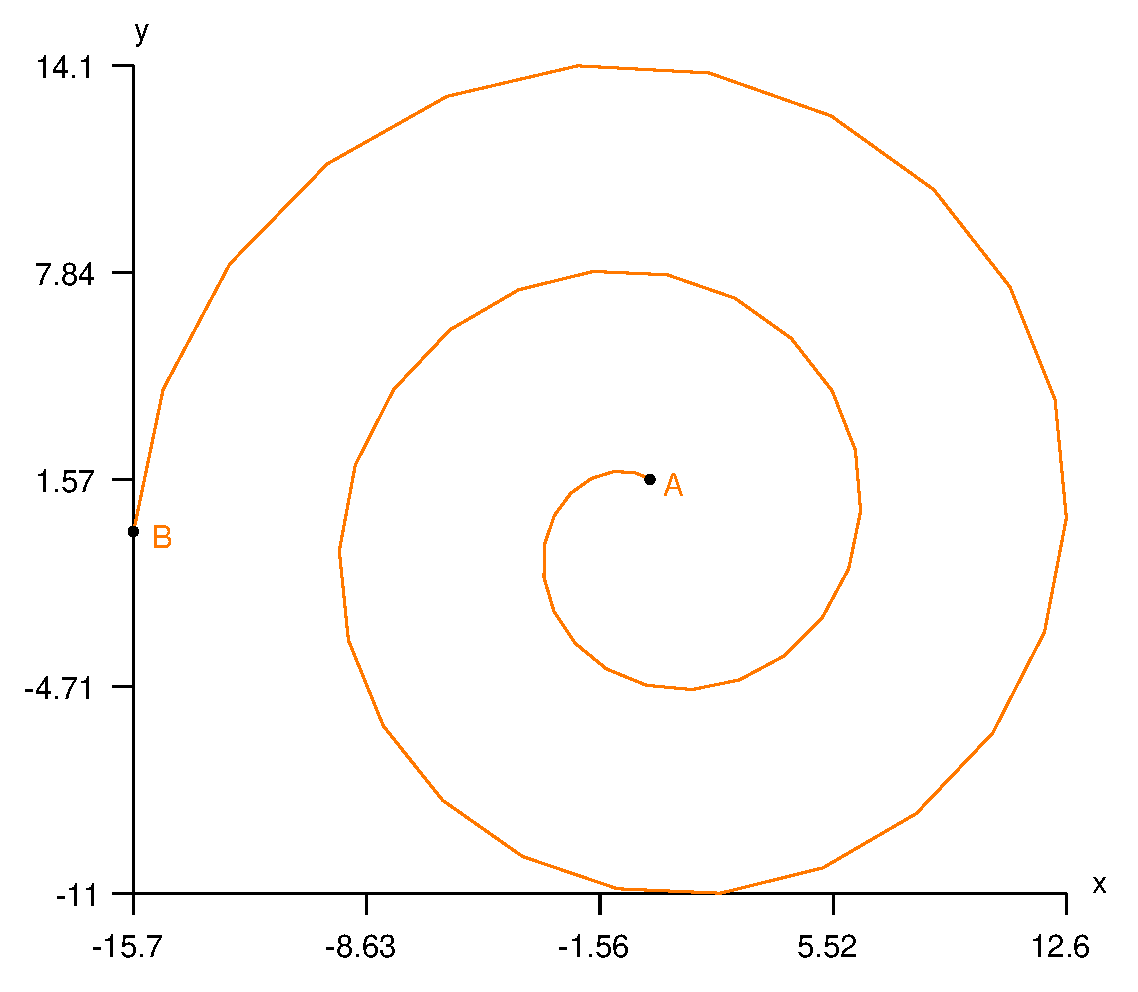
\includegraphics[width=60mm]{spiral}
  \caption{One-dimensional mesh in $ {\mathbb R}^2 $}
\end{figure}

The operator {\small\tt \&\&} joins two functions into one vector-valued function.

Note that, when defining points {\small\tt A} and {\small\tt B}, we only set the value of
{\small\tt t}.
Functions {\small\tt x} and {\small\tt y} are defined later, as arithmetic expressions in terms of
{\small\tt t}; their values will be computed ``on-the-fly'' when needed.
%A parametric manifold has attached to it a function called ``parameter'' and another one called
%``coordinate''.
%Both may be vector functions (may have serveral components).
%The ``coordinates'' are used, for instance, for graphical representation.
%The ``parameter'' or ``parameters'' are used, for instance, for interpolation.
%The {\small\tt\verm{Mesh}} constructors with {\small\tt\textcolor{tag}{tag}::segment},
%{\small\tt\textcolor{tag}{tag}::quadrangle} or {\small\tt\textcolor{tag}{tag}::triangle}
% build new points and define their position in the manifold by
%interpolating the parameters, not the coordinates.
%Unlike for implicit manifolds, no projection is necessary.
In the drawing above, we note that the generated points are not equidistant in the sense of the
Euclidian distance in $ \mathbb{R}^2 $.
They correspond to values of {\small\tt t} which are uniformly distributed between
$ \pi/2 $ (at {\small\tt A}) and $ 5\pi $ (at {\small\tt B}).

The approach described above has the disadvantage that, if we want to subsequently change the
distribution of nodes along the {\small\tt arc\_\,of\_\,spiral}, we must switch back to the original
{\small\tt t} coordinate.

Paragraph \ref{\numb section 3.\numb parag 5} shows another way of meshing a curve,
producing equidistant vertices.


          %----------------%
\section{~~Closing a circle}\label{\numb section 2.\numb parag 16}
          %----------------%

In the approach of paragraph \ref{\numb section 2.\numb parag 15}, it is possible but cumbersome to
build a closed curve :

\begin{Verbatim}[commandchars=\\\{\},formatcom=\small\tt,frame=single,
   label=parag-\ref{\numb section 2.\numb parag 16}.cpp,rulecolor=\color{coment},
   baselinestretch=0.94,framesep=2mm]
   \verm{Manifold} \azul{circle_manif} ( \textcolor{tag}{tag}::Euclid, \textcolor{tag}{tag}::of_dim, \laranja{1} );
   \verm{Function} \azul{t} = circle_manif .build_coordinate_system
      ( \textcolor{tag}{tag}::Lagrange, \textcolor{tag}{tag}::of_degree, \laranja{1} );

   \cinza{// build 'circle' merely as a segment from 0 to 1.9 pi}
   const double \azul{pi} = \laranja{3.1415926536};
   \verm{Cell} \azul{A} ( \textcolor{tag}{tag}::vertex );  t(A) =  \laranja{0.};
   \verm{Cell} \azul{B} ( \textcolor{tag}{tag}::vertex );  t(B) =  \laranja{1.9}*pi;
   \verm{Mesh} \azul{incomplete_circle} ( \textcolor{tag}{tag}::segment, A .reverse(), B, \textcolor{tag}{tag}::divided_in, \laranja{19} );

   \cinza{// now close the curve in a not very elegant manner}
   \verm{Mesh} \azul{small_piece} ( \textcolor{tag}{tag}::segment, B .reverse(), A, \textcolor{tag}{tag}::divided_in, \laranja{1} );
   \verm{Mesh} \azul{circle} ( \textcolor{tag}{tag}::join, incomplete_circle, small_piece );
   \cinza{// define new coordinates on circle_manif as expressions of t :}
   \verm{Function} \azul{x} = \verm{cos}(t), \azul{y} = \verm{sin}(t);
   \verm{Manifold} \azul{RR2} ( tag::Euclid, \textcolor{tag}{tag}::of_dimension, \laranja{2} );
   RR2 .set_coordinates ( x && y );

   \cinza{// in future statements (e.g. for graphical representation)}
   \cinza{// x and y will be used, not t :}
   circle .draw_ps (\verde{"circle.eps"});
\end{Verbatim}

Paragraph \ref{\numb section 7.\numb parag 2} shows a more elegant way to close a curve in itself.

On the other hand, if we only want a visual illusion of a closed circle, we may use the code below.

\begin{Verbatim}[commandchars=\\\{\},formatcom=\small\tt,baselinestretch=0.94]
   \verm{Manifold} \azul{circle_manif} ( \textcolor{tag}{tag}::Euclid, \textcolor{tag}{tag}::of_dim, \laranja{1} );
   \verm{Function} \azul{t} = circle_manif .build_coordinate_system
      ( \textcolor{tag}{tag}::Lagrange, \textcolor{tag}{tag}::of_degree, \laranja{1} );

   \cinza{// build 'circle' merely as a segment from 0 to 2 pi}
   const double \azul{pi} = \laranja{3.1415926536};
   \verm{Cell} \azul{A} ( \textcolor{tag}{tag}::vertex );  t (A) = \laranja{0.};
   \verm{Cell} \azul{B} ( \textcolor{tag}{tag}::vertex );  t (B) = \laranja{2.}*pi;
   \verm{Mesh} \azul{circle} ( \textcolor{tag}{tag}::segment, A .reverse(), B, \textcolor{tag}{tag}::divided_in, \laranja{20} );
   \cinza{// gives the illusion of a closed circle}

   \cinza{// define new coordinates on circle_manif as expressions of t :}
   \verm{Function} \azul{x} = \verm{cos}(t), \azul{y} = \verm{sin}(t);
   \verm{Manifold} \azul{RR2} ( tag::Euclid, \textcolor{tag}{tag}::of_dimension, \laranja{2} );
   RR2 .set_coordinates ( x && y );
\end{Verbatim}


          %---------------------------------%
\section{~~Parametric manifolds -- a surface}\label{\numb section 2.\numb parag 17}
          %---------------------------------%

Here is an example of a parametrized surface :

\begin{figure}[ht] \centering
  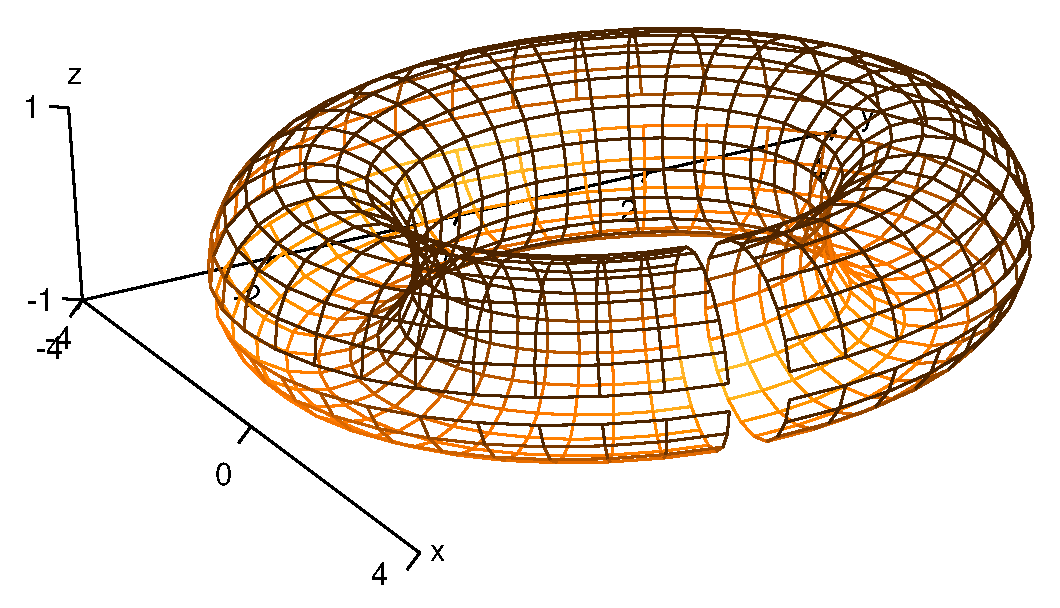
\includegraphics[width=105mm]{torus}
  \caption{Incomplete torus}
\end{figure}

\begin{Verbatim}[commandchars=\\\{\},formatcom=\small\tt,frame=single,
   label=parag-\ref{\numb section 2.\numb parag 17}.cpp,rulecolor=\color{coment},
   baselinestretch=0.94,framesep=2mm]
   \verm{Manifold} \azul{torus} ( \textcolor{tag}{tag}::Euclid, \textcolor{tag}{tag}::of_dim, \laranja{2} );
   \verm{Function} \azul{alpha_beta} =
      torus .build_coordinate_system ( \textcolor{tag}{tag}::Lagrange, \textcolor{tag}{tag}::of_degree, \laranja{1} );

   \cinza{// extract components of alpha_beta :}
   \verm{Function} \azul{alpha} = alpha_beta [0], \azul{beta} = alpha_beta [1];

   \cinza{// build a rectangle in the alpha-beta plane}
   const double \azul{pi} = \laranja{3.1415926536};
   \verm{Cell} \azul{A} ( \textcolor{tag}{tag}::vertex );  alpha (A) = \laranja{0.};       beta (A) = \laranja{0.};
   \verm{Cell} \azul{B} ( \textcolor{tag}{tag}::vertex );  alpha (B) = \laranja{0.};       beta (B) = \laranja{1.9}*pi;
   \verm{Cell} \azul{C} ( \textcolor{tag}{tag}::vertex );  alpha (C) = \laranja{1.95}*pi;  beta (C) = \laranja{1.9}*pi;
   \verm{Cell} \azul{D} ( \textcolor{tag}{tag}::vertex );  alpha (D) = \laranja{1.95}*pi;  beta (D) = \laranja{0.};

   \cinza{// four almost-closed circles :}
   \verm{Mesh} \azul{AB} ( \textcolor{tag}{tag}::segment, A .reverse(), B, \textcolor{tag}{tag}::divided_in, \laranja{19} );
   \verm{Mesh} \azul{BC} ( \textcolor{tag}{tag}::segment, B .reverse(), C, \textcolor{tag}{tag}::divided_in, \laranja{39} );
   \verm{Mesh} \azul{CD} ( \textcolor{tag}{tag}::segment, C .reverse(), D, \textcolor{tag}{tag}::divided_in, \laranja{19} );
   \verm{Mesh} \azul{DA} ( \textcolor{tag}{tag}::segment, D .reverse(), A, \textcolor{tag}{tag}::divided_in, \laranja{39} );
   \verm{Mesh} \azul{ABCD} ( \textcolor{tag}{tag}::rectangle, AB, BC, CD, DA );  \cinza{// an almost-closed torus}
   
   \cinza{// parametrize the torus}
   const double \azul{big_radius} = \laranja{3.}, \azul{small_radius} = \laranja{1.};
   \verm{Function} \azul{x} = ( big_radius + small_radius * \verm{cos}(beta) ) * \verm{cos}(alpha),
            \azul{y} = ( big_radius + small_radius * \verm{cos}(beta) ) * \verm{sin}(alpha),
            \azul{z} = small_radius * \verm{sin}(beta);

   \verm{Manifold} \azul{RR3} ( tag::Euclid, \textcolor{tag}{tag}::of_dimension, \laranja{3} );
   RR3 .set_coordinates ( x && y && z );  \cinza{// forget about alpha and beta}
   \cinza{// in future statements (e.g. for graphical representation)}
   \cinza{// x, y and z will be used, not alpha nor beta :}
   ABCD .export_to_file ( \textcolor{tag}{tag}::msh, \verde{"torus.msh"});
\end{Verbatim}

Closing the torus in the cumbersome manner shown in paragraph
\ref{\numb section 2.\numb parag 16} is possible but not practical.
Paragraph \ref{\numb section 7.\numb parag 5} shows a more elegant solution.

If we only want a visual illusion of a closed surface, we may use the code below

\begin{Verbatim}[commandchars=\\\{\},formatcom=\small\tt,baselinestretch=0.94]
   \verm{Cell} \azul{A} ( \textcolor{tag}{tag}::vertex );  alpha (A) = \laranja{0.};     beta (A) = \laranja{0.};
   \verm{Cell} \azul{B} ( \textcolor{tag}{tag}::vertex );  alpha (B) = \laranja{0.};     beta (B) = \laranja{2.}*pi;
   \verm{Cell} \azul{C} ( \textcolor{tag}{tag}::vertex );  alpha (C) = \laranja{2.}*pi;  beta (C) = \laranja{2.}*pi;
   \verm{Cell} \azul{D} ( \textcolor{tag}{tag}::vertex );  alpha (D) = \laranja{2.}*pi;  beta (D) = \laranja{0.};

   \verm{Mesh} \azul{AB} ( \textcolor{tag}{tag}::segment, A .reverse(), B, \textcolor{tag}{tag}::divided_in, \laranja{20} );
   \verm{Mesh} \azul{BC} ( \textcolor{tag}{tag}::segment, B .reverse(), C, \textcolor{tag}{tag}::divided_in, \laranja{40} );
   \verm{Mesh} \azul{CD} ( \textcolor{tag}{tag}::segment, C .reverse(), D, \textcolor{tag}{tag}::divided_in, \laranja{20} );
   \verm{Mesh} \azul{DA} ( \textcolor{tag}{tag}::segment, D .reverse(), A, \textcolor{tag}{tag}::divided_in, \laranja{40} );
   \cinza{// AB, BC, CD and DA look like closed circles}

   \verm{Mesh} \azul{ABCD} ( \textcolor{tag}{tag}::rectangle, AB, BC, CD, DA );
   \cinza{// ABCD gives the illusion of a closed torus}
\end{Verbatim}


          %-----------------------------------------%
\section{~~Starting with a high-dimensional manifold}\label{\numb section 2.\numb parag 18}
          %-----------------------------------------%

Instead of starting with a manifold having only the parameter(s), we may start with a
high-dimensional manifold containing both the geometric coordinates and the parameter(s),
then define the parametrization through equation(s).
% The advantage of this approach is that we can later shwitch on and off a constraint,
% thus switching between meshes of different dimensions.
There is a disadvantage however, regarding performance : {\maniFEM} will reserve,
for each vertex, space in the computer's memory for five {\small\tt double} values.

\begin{Verbatim}[commandchars=\\\{\},formatcom=\small\tt,frame=single,
   label=parag-\ref{\numb section 2.\numb parag 18}.cpp,rulecolor=\color{coment},
   baselinestretch=0.94,framesep=2mm]
   \verm{Manifold} \azul{RR5} ( \textcolor{tag}{tag}::Euclid, \textcolor{tag}{tag}::of_dim, \laranja{5} );
   \verm{Function} \azul{xyzab} = RR5 .build_coordinate_system ( \textcolor{tag}{tag}::Lagrange, \textcolor{tag}{tag}::of_degree, \laranja{1} );

   \cinza{// extract components of xyzab :}
   \verm{Function} \azul{x} = xyzab [\laranja{0}], \azul{y} = xyzab [\laranja{1}], \azul{z} = xyzab [\laranja{2}],
             \azul{alpha} = xyzab [\laranja{3}], \azul{beta} = xyzab [\laranja{4}];

   \cinza{// define a torus as a submanifold of RR5 :}
   const double \azul{big_radius} = \laranja{3}, \azul{small_radius} = \laranja{1};
   \verm{Manifold} \azul{torus} = RR5 .parametric
      ( x == ( big_radius + small_radius * \verm{cos}(beta) ) * \verm{cos}(alpha),
        y == ( big_radius + small_radius * \verm{cos}(beta) ) * \verm{sin}(alpha),
        z == small_radius * \verm{sin}(beta)                                );
        
   \cinza{// define four corners :}
   const double \azul{pi} = \laranja{3.1415926536};
   \verm{Cell} \azul{A} ( \textcolor{tag}{tag}::vertex );  alpha (A) = \laranja{0.};       beta (A) = \laranja{0.};
   torus .project (A);
   \verm{Cell} \azul{B} ( \textcolor{tag}{tag}::vertex );  alpha (B) = \laranja{0.};       beta (B) = \laranja{1.9}*pi;
   torus .project (B);
   \verm{Cell} \azul{C} ( \textcolor{tag}{tag}::vertex );  alpha (C) = \laranja{1.95}*pi;  beta (C) = \laranja{1.9}*pi;
   torus .project (C);
   \verm{Cell} \azul{D} ( \textcolor{tag}{tag}::vertex );  alpha (D) = \laranja{1.95}*pi;  beta (D) = \laranja{0.};
   torus .project (D);

   \cinza{// four almost-closed circles :}
   \verm{Mesh} \azul{AB} ( \textcolor{tag}{tag}::segment, A .reverse(), B, \textcolor{tag}{tag}::divided_in, \laranja{19} );
   \verm{Mesh} \azul{BC} ( \textcolor{tag}{tag}::segment, B .reverse(), C, \textcolor{tag}{tag}::divided_in, \laranja{39} );
   \verm{Mesh} \azul{CD} ( \textcolor{tag}{tag}::segment, C .reverse(), D, \textcolor{tag}{tag}::divided_in, \laranja{19} );
   \verm{Mesh} \azul{DA} ( \textcolor{tag}{tag}::segment, D .reverse(), A, \textcolor{tag}{tag}::divided_in, \laranja{39} );

   \cinza{// build a rectangle}
   \verm{Mesh} \azul{ABCD} ( \textcolor{tag}{tag}::rectangle, AB, BC, CD, DA );  \cinza{// an almost-closed torus}

   \verm{Manifold} \azul{RR3} ( tag::Euclid, \textcolor{tag}{tag}::of_dimension, \laranja{3} );
   RR3 .set_coordinates ( x && y && z );  \cinza{// forget about alpha and beta}

   \cinza{// in future statements (e.g. for graphical representation)}
   \cinza{// x, y and z will be used, not alpha nor beta :}
   ABCD .export_to_file ( \textcolor{tag}{tag}::msh, \verde{"torus.msh"});
\end{Verbatim}

The {\small\tt\verm{Manifold}::parametric} method is similar to {\small\tt\verm{Manifold}::implicit},
presented in paragraphs \ref{\numb section 2.\numb parag 4} --
\ref{\numb section 2.\numb parag 14}.
The only difference is that by using {\small\tt parametric} we declare an explicit dependence%
\footnote {Perhaps {\small\tt explicit} would be a better name than {\small\tt parametric};
unfortunately, that word is reserved in {\small\tt C++}.}
of the coordinates (here, {\small\tt x}, {\small\tt y} and {\small\tt z}) upon the parameters
(here, {\small\tt alpha} and {\small\tt beta}).
This endows the manifold {\small\tt torus} with a different projection operator.
The projection of a vertex from {\small\tt RR5} onto {\small\tt torus} is done by merely updating
the values of {\small\tt x}, {\small\tt y} and {\small\tt z}, while keeping {\small\tt alpha} and
{\small\tt beta} constant.


          %-------------------------------------%
\chapter{~~Frontal mesh generation; knitting}\label{\numb section 3}
          %-------------------------------------%

Section \ref{\numb section 2} shows how to build meshes by joining together several regular meshes
(triangles or quadrangles), like patches.
The present section explains how to build a mesh by gradually adding cells, on by one.
We call this approach ``frontal mesh generation'' because we gradually propagate a front of segments.
In some cases, the process starts with a given interface and adds triangles, one by one,
moving and deforming the interface, until it shrinks and disappears.
In other cases (like in paragraphs \ref{\numb section 3.\numb parag 2},
\ref{\numb section 3.\numb parag 4}, \ref{\numb section 3.\numb parag 6},
\ref{\numb section 3.\numb parag 7}) we begin with nothing at all;
{\maniFEM} finds a starting point by itself.

Frontal mesh generation works with segment cells (for one-dimensional meshes) and
triangular cells (for two-dimensional meshes).
Meshing of three-dimensional domains will be implemented in the future and will use tetrahedral
cells.

Frontal mesh generation follows the shape of the current working manifold (the most recently
declared {\small\tt\verm{Manifold}} object) by {\small\tt project}ing each newly constructed vertex
on that manifold.
Recall that in this manual we use the term ``manifold'' to mean a manifold without boundary.


          %--------------%
\section{~~Filling a disk}\label{\numb section 3.\numb parag 1}
          %--------------%

Paragraph \ref{\numb section 2.\numb parag 9} shows how to build a mesh over a disk,
but the quality of the mesh is quite poor.
This is so because the {\small\tt\verm{Mesh}} constructor with
{\small\tt\textcolor{tag}{tag}::quadrangle} treats the disk as a (much) deformed rectangle.

We can ask {\maniFEM} to mesh the disk, starting from its boundary (a circle)
and adding triangles, one by one, until the disk is completely covered :

\begin{figure} \centering
 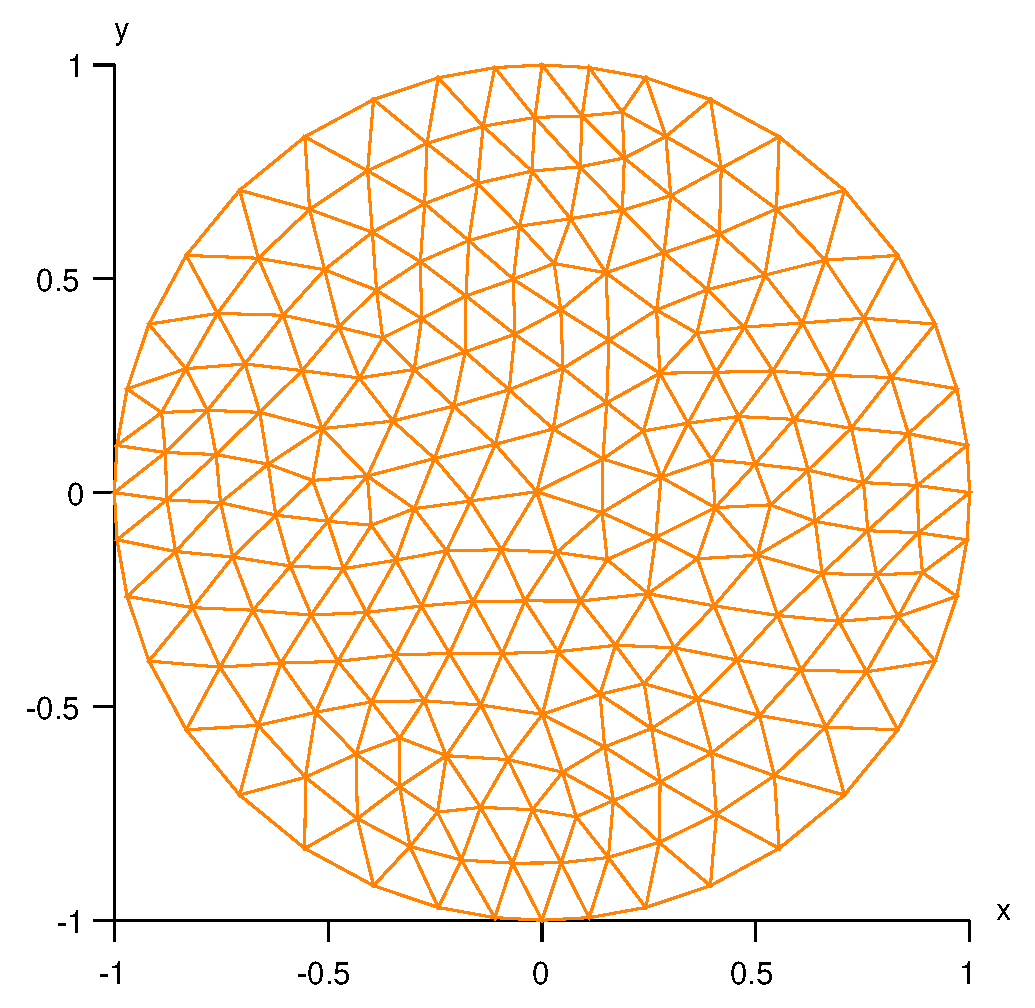
\includegraphics[width=85mm]{disk-with-tri}
 \caption{Circle built from patches, interior of disk meshed with frontal method}
 \label{\numb section 3.\numb fig 1}
\end{figure}

\begin{Verbatim}[commandchars=\\\{\},formatcom=\small\tt,frame=single,
   label=parag-\ref{\numb section 3.\numb parag 1}.cpp,rulecolor=\color{moldura},
   baselinestretch=0.94,framesep=2mm                                            ]
   \verm{Manifold} \azul{RR2} ( \textcolor{tag}{tag}::Euclid, \textcolor{tag}{tag}::of_dim, \laranja{2} );
   \verm{Function} \azul{xy} = RR2 .build_coordinate_system ( \textcolor{tag}{tag}::Lagrange, \textcolor{tag}{tag}::of_degree, \laranja{1} );
   \verm{Function} \azul{x} = xy [\laranja{0}], \azul{y} = xy [\laranja{1}];
   
   \verm{Manifold} \azul{circle_manif} = RR2 .implicit ( x*x + y*y == \laranja{1.} );
   
   \verm{Cell} \azul{N} ( \textcolor{tag}{tag}::vertex );  x (N) =  \laranja{0.};   y (N) =  \laranja{1.};
   \verm{Cell} \azul{W} ( \textcolor{tag}{tag}::vertex );  x (W) = \laranja{-1.};   y (W) =  \laranja{0.};
   \verm{Cell} \azul{S} ( \textcolor{tag}{tag}::vertex );  x (S) =  \laranja{0.};   y (S) = \laranja{-1.};
   \verm{Cell} \azul{E} ( \textcolor{tag}{tag}::vertex );  x (E) =  \laranja{1.};   y (E) =  \laranja{0.};
   \verm{Mesh} \azul{NW} ( \textcolor{tag}{tag}::segment, N .reverse(), W, \textcolor{tag}{tag}::divided_in, \laranja{10} );
   \verm{Mesh} \azul{WS} ( \textcolor{tag}{tag}::segment, W .reverse(), S, \textcolor{tag}{tag}::divided_in, \laranja{10} );
   \verm{Mesh} \azul{SE} ( \textcolor{tag}{tag}::segment, S .reverse(), E, \textcolor{tag}{tag}::divided_in, \laranja{10} );
   \verm{Mesh} \azul{EN} ( \textcolor{tag}{tag}::segment, E .reverse(), N, \textcolor{tag}{tag}::divided_in, \laranja{10} );
   \verm{Mesh} \azul{circle} ( \textcolor{tag}{tag}::join, NW, WS, SE, EN );
   
   RR2 .set_as_working_manifold();
   \verm{Mesh} \azul{disk} ( \textcolor{tag}{tag}::frontal, \textcolor{tag}{tag}::boundary, circle, \textcolor{tag}{tag}::desired_length, \laranja{0.157} );
\end{Verbatim}

We provide the desired length of the segments of the future mesh as an argument to the
constructor.
Of course the length of the segments inside the mesh will vary slightly.
We must take care to give as boundary a curve with segments of length approximatively equal
to the desired length (paragraph \ref{\numb section 3.\numb parag 16} discusses
this requirement).

Paragraph \ref{\numb section 11.\numb parag 2} explains the coloring conventions observed
in this manual for {\tt C++} code.
Paragraph \ref{\numb section 11.\numb parag 3} gives details about {\small\tt\textcolor{tag}{tag}}s.


          %----------------%
\section{~~Meshing a circle}\label{\numb section 3.\numb parag 2}
          %----------------%

Instead of building the circle by joining four (curved) segments, we can mesh directly
the circle manifold, then mesh the disk :

\begin{Verbatim}[commandchars=\\\{\},formatcom=\small\tt,frame=single,
   label=parag-\ref{\numb section 3.\numb parag 2}.cpp,rulecolor=\color{moldura},
   baselinestretch=0.94,framesep=2mm                                            ]
   \verm{Manifold} \azul{RR2} ( \textcolor{tag}{tag}::Euclid, \textcolor{tag}{tag}::of_dim, \laranja{2} );
   \verm{Function} \azul{xy} = RR2 .build_coordinate_system ( \textcolor{tag}{tag}::Lagrange, \textcolor{tag}{tag}::of_degree, \laranja{1} );
   \verm{Function} \azul{x} = xy [\laranja{0}], \azul{y} = xy [\laranja{1}];
   
   \verm{Manifold} \azul{circle_manif} = RR2 .implicit ( x*x + y*y == \laranja{1.} );
   \verm{Mesh} \azul{circle} ( \textcolor{tag}{tag}::frontal,
                 \textcolor{tag}{tag}::entire_manifold, circle_manif, \textcolor{tag}{tag}::desired_length, \laranja{0.2} );
   \cinza{// we can omit the manifold; maniFEM will take the current working manifold :}
   \cinza{// Mesh circle ( tag::frontal, tag::desired_length, 0.2 );}
   
   RR2 .set_as_working_manifold();
   \verm{Mesh} \azul{disk} ( \textcolor{tag}{tag}::frontal, \textcolor{tag}{tag}::boundary, circle, \textcolor{tag}{tag}::desired_length, \laranja{0.2} );
   disk .draw_ps (\verde{"disk.eps"});
\end{Verbatim}

The code above is quite comfortable for the user; he or she only needs to define
the manifold(s) to be meshed and provide the desired (average) length of segments
in the future mesh.
However, this comfort comes at the price of a significant computational effort.
For building the {\small\tt circle}, {\ManiFEM} must first find a starting point for the process
of frontal mesh generation.
In extreme cases, the algorithm may fail to find a starting point on the given manifold.

The user may choose to be more specific in order to save computation time,
by providing a starting point :

\begin{Verbatim}[commandchars=\\\{\},formatcom=\small\tt,
   baselinestretch=0.94,framesep=2mm                      ]
   \verm{Cell} \azul{A} ( \textcolor{tag}{tag}::vertex );  x (A) = \laranja{1.};  y (A) = \laranja{0.};
   \verm{Mesh} \azul{circle} ( \textcolor{tag}{tag}::frontal, \textcolor{tag}{tag}::start_at, A, \textcolor{tag}{tag}::desired_length, \laranja{0.2} );
\end{Verbatim}

Also, {\maniFEM} must infer the right orientation of the {\small\tt circle}
as explained in paragraphs \ref{\numb section 3.\numb parag 10} and
\ref{\numb section 3.\numb parag 13}.
Choosing the other orientation would result in an endless process of meshing the exterior of
the disk.
The process of choosing the right orientation implies some computational effort.
The user can make things easier for {\maniFEM} either by attaching an orientation
to the manifold {\small\tt circle\_\,manif} (this feature is not implemented yet) or
by providing the initial direction as shown in paragraph \ref{\numb section 3.\numb parag 12}.


          %----------------%
\section{~~Inner boundaries}\label{\numb section 3.\numb parag 3}
          %----------------%

Inner boundaries must have the reverse orientation :

\begin{Verbatim}[commandchars=\\\{\},formatcom=\small\tt,frame=single,
   label=parag-\ref{\numb section 3.\numb parag 3}.cpp,rulecolor=\color{moldura},
   baselinestretch=0.94,framesep=2mm                                            ]
   \verm{Manifold} \azul{circle} = RR2 .implicit ( x*x + y*y == \laranja{1.} );
   \verm{Mesh} \azul{outer} ( \textcolor{tag}{tag}::frontal, \textcolor{tag}{tag}::desired_length, \laranja{0.1} );
   \verm{Manifold} \azul{ellipse} = RR2 .implicit ( x*x + (y-\laranja{0.37})*(y-\laranja{0.37}) + \laranja{0.3}*x*y == \laranja{0.25} );
   \verm{Mesh} \azul{inner} ( \textcolor{tag}{tag}::frontal, \textcolor{tag}{tag}::desired_length, \laranja{0.1} );
   \verm{Mesh} \azul{bdry} ( \textcolor{tag}{tag}::join, outer, inner .reverse() );
   RR2 .set_as_working_manifold();
   \verm{Mesh} \azul{disk} ( \textcolor{tag}{tag}::frontal, \textcolor{tag}{tag}::boundary, bdry, \textcolor{tag}{tag}::desired_length, \laranja{0.1} );
\end{Verbatim}

\begin{figure}[ht] \centering
 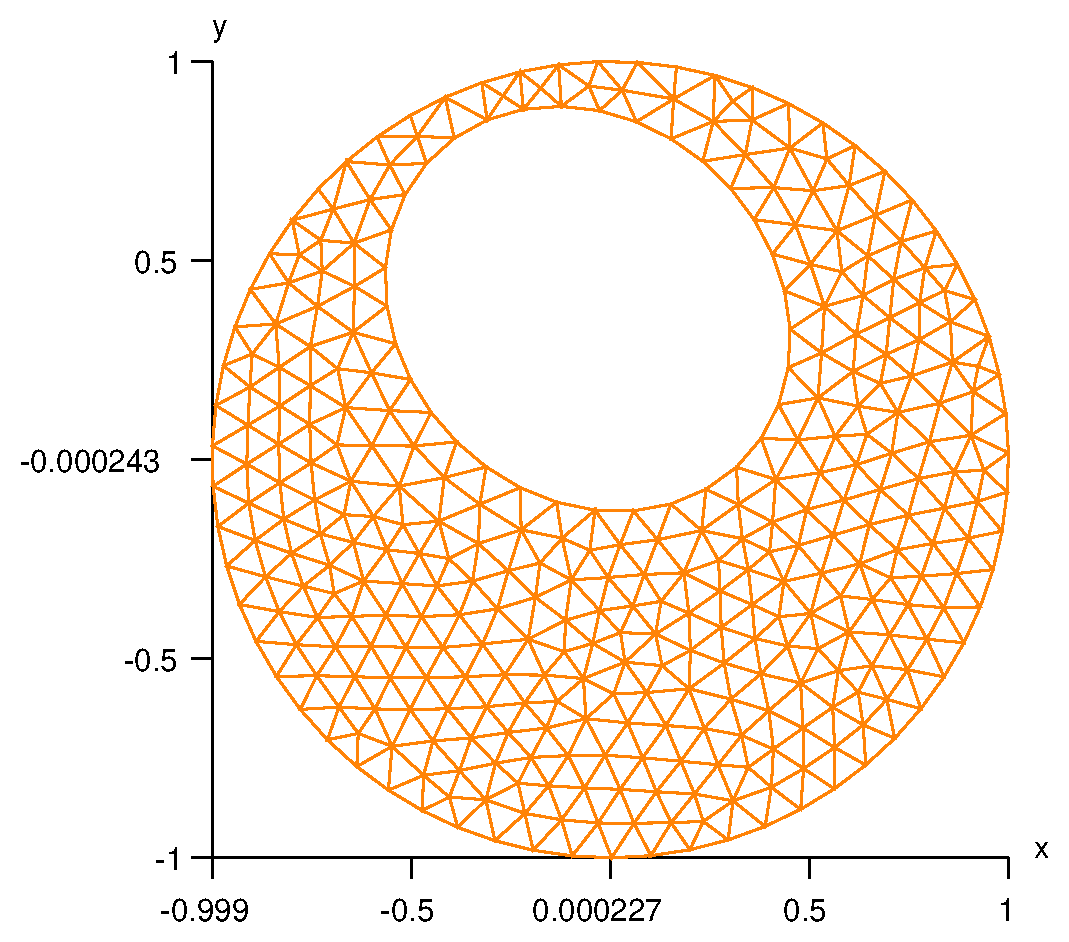
\includegraphics[width=95mm]{disk-with-hole}
  \caption{Disk with a hole}
  \label{\numb section 3.\numb fig 2}
\end{figure}

Paragraphs \ref{\numb section 1.\numb parag 2} and \ref{\numb section 1.\numb parag 4} explain
the relation between the orientation of a mesh and the orientation of its boundary.

Paragraphs \ref{\numb section 3.\numb parag 10} and \ref{\numb section 3.\numb parag 13}
explain how {\maniFEM} chooses the orientation of closed curves.


          %--------------------------------%
\section{~~Meshing a three-dimensional loop}\label{\numb section 3.\numb parag 4}
          %--------------------------------%

We may apply the same {\small\tt frontal} algorithm for meshing the circle in
$ \mathbb{R}^3 $ introduced in paragraph \ref{\numb section 2.\numb parag 15} :

\begin{Verbatim}[commandchars=\\\{\},formatcom=\small\tt,frame=single,
   label=parag-\ref{\numb section 3.\numb parag 4}.cpp,rulecolor=\color{moldura},
   baselinestretch=0.94,framesep=2mm                                            ]
   \verm{Manifold} \azul{RR3} ( \textcolor{tag}{tag}::Euclid, \textcolor{tag}{tag}::of_dim, \laranja{3} );
   \verm{Function} \azul{xyz} = RR3 .build_coordinate_system ( \textcolor{tag}{tag}::Lagrange, \textcolor{tag}{tag}::of_degree, \laranja{1} );
   \verm{Function} \azul{x} = xyz [\laranja{0}], \azul{y} = xyz [\laranja{1}], \azul{z} = xyz [\laranja{2}];
   \verm{Manifold} \azul{circle_manif} = RR3 .implicit ( x*x + y*y == \laranja{1.}, x*y == \laranja{4.}*z );
   
   \verm{Mesh} \azul{circle} ( \textcolor{tag}{tag}::frontal, \textcolor{tag}{tag}::desired_length, \laranja{0.1},
                 \textcolor{tag}{tag}::orientation, \textcolor{tag}{tag}::random          );
\end{Verbatim}

Unlike for the {\small\tt circle} in paragraph \ref{\numb section 3.\numb parag 2},
there is no way to choose between the two possible orientations of this {\small\tt circle}.
No one is more ``correct'' than the other.
This is why {\maniFEM} requires supplementary arguments
{\small\tt\textcolor{tag}{tag}::orientation,} {\small\tt\textcolor{tag}{tag}::random}
for the {\small\tt\verm{Mesh}} constructor.
In other cases (e.g.\ for closed curves in $ \mathbb{R}^2 $) these supplementary arguments
are not mandatory; however, even then the user may choose to provide them,
thus sparing the computer from the burden of finding the right orientation.
Paragraphs \ref{\numb section 3.\numb parag 10} and \ref{\numb section 3.\numb parag 13}
give more details.

The term ``random'' should not be interpreted in the probabilistic sense.
The orientation of such a mesh is not a random variable, not even a pseudo-random one.
Is it just difficult to predict.

On the other hand, if the orientation matters for you, you can either attach an orientation
to the manifold {\small\tt circle\_\,manif} (this feature is not implemented yet)
or provide a starting point and an initial direction as shown in paragraph
\ref{\numb section 3.\numb parag 12}.


          %----------------------------%
\section{~~Starting and stopping points}\label{\numb section 3.\numb parag 5}
          %----------------------------%

In paragraphs \ref{\numb section 3.\numb parag 2} and \ref{\numb section 3.\numb parag 4}
we have meshed the entire closed curve {\small\tt circle}.
If we only want a piece of a curve, we must specify two points, one for starting and
the other one for stopping.

Looking at the example in paragraph \ref{\numb section 2.\numb parag 18}, let us define a
spiral with a slightly different look and switch to frontal mesh generation.

\begin{Verbatim}[commandchars=\\\{\},formatcom=\small\tt,frame=single,
   label=parag-\ref{\numb section 3.\numb parag 5}.cpp,rulecolor=\color{moldura},
   baselinestretch=0.94,framesep=2mm                                            ]
   \verm{Manifold} \azul{RR2} ( \textcolor{tag}{tag}::Euclid, \textcolor{tag}{tag}::of_dim, \laranja{2} );
   \verm{Function} \azul{xy} = RR2 .build_coordinate_system ( \textcolor{tag}{tag}::Lagrange, \textcolor{tag}{tag}::of_degree, \laranja{1} );
   \verm{Function} \azul{x} = xy [\laranja{0}], \azul{y} = xy [\laranja{1}];
   \verm{Function} \azul{r} = \verm{power} ( x*x + y*y, \laranja{0.25} );
   const double \azul{pi} = \laranja{3.14159};
   
   RR2 .implicit ( x*\verm{sin}(r) == y*\verm{cos}(r) );
   \cinza{// we don't need to give a name to the implicit manifold}
   \cinza{// the Manifold constructor sets the manifold it builds as working manifold}
   \cinza{// after that, many methods use this working manifold by default}
   
   \verm{Cell} \azul{A} ( \textcolor{tag}{tag}::vertex );  x (A) =     pi*pi;   y (A) = \laranja{0.};
   \verm{Cell} \azul{B} ( \textcolor{tag}{tag}::vertex );  x (B) = \laranja{81.}*pi*pi;   y (B) = \laranja{0.};
   \verm{Mesh} \azul{spiral} ( \textcolor{tag}{tag}::frontal, \textcolor{tag}{tag}::start_at, A, \textcolor{tag}{tag}::stop_at, B,
                 \textcolor{tag}{tag}::desired_length, \laranja{1.}, \textcolor{tag}{tag}::shortest_path     );
\end{Verbatim}

\begin{figure} \centering
  \psfrag{A}{\tt\textcolor{textindraw}{A}}
  \psfrag{B}{\tt\textcolor{textindraw}{B}}
 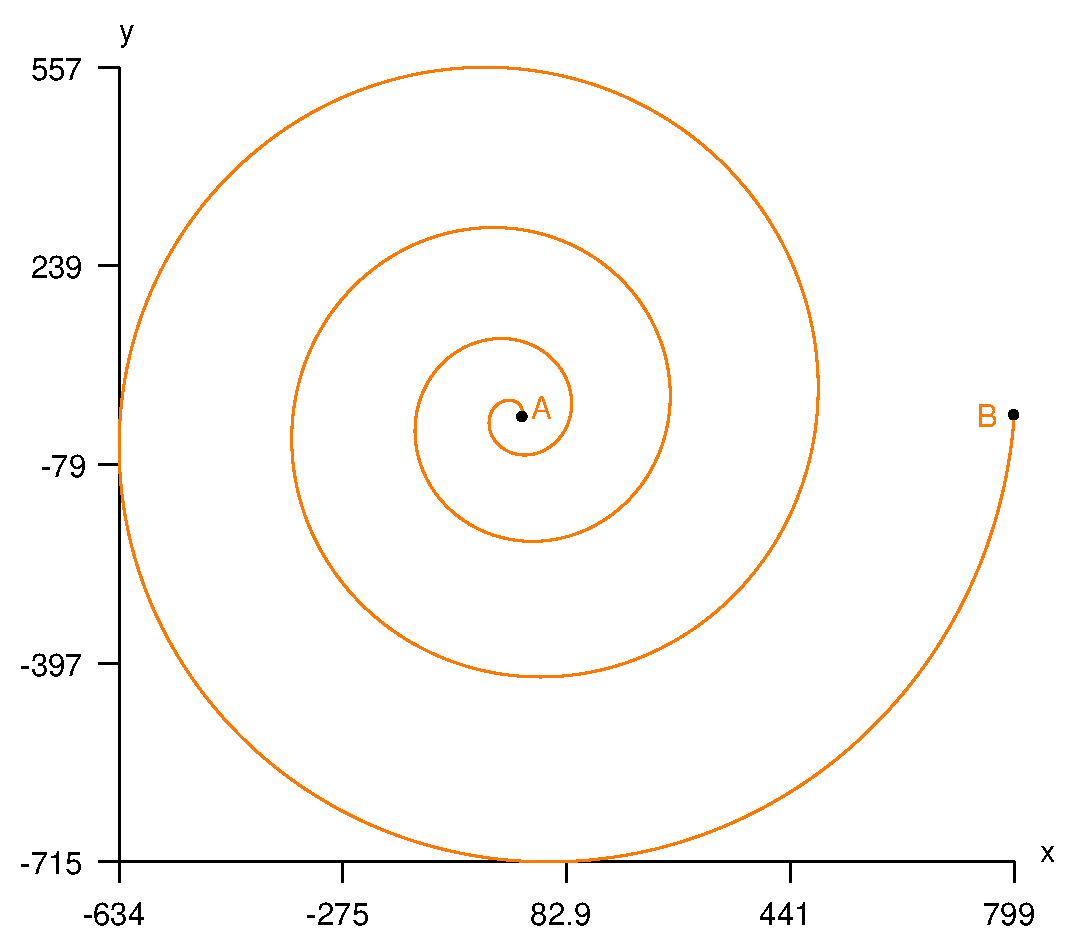
\includegraphics[width=75mm]{spiral-prog}
  \caption{Spiral, meshed by frontal method}
 \label{\numb section 3.\numb fig 3}
\end{figure}

Figure \ref{\numb section 3.\numb fig 3} shows the resulting mesh.

Unlike in paragraph \ref{\numb section 2.\numb parag 18}, we define the spiral through
an implicit equation.
Had we chosen the (natural) definition {\small\tt r = \verm{power} ( x*x + y*y, 0.5 )},
the very same spiral as in paragraph \ref{\numb section 2.\numb parag 18} would have been
obtained.
For aesthetic reasons, we have chosen a different definition of {\small\tt r}, thus obtaining
a different spacing between the arcs of the spiral.

Another noteworthy difference from paragraph \ref{\numb section 2.\numb parag 18} is that
vertices are distributed uniformly along the spiral (with respect to the distance
in the surrounding space $ \mathbb{R}^2 $).
The segments are too small to be seen in the figure.

Note that there are two ways to go along the spiral starting from {\small\tt A}.
One of them will eventually stumble upon the stopping point {\small\tt B} while
the other one will never meet {\small\tt B}.
{\ManiFEM} has no means to guess which way it should start building the mesh;
the {\small\tt\textcolor{tag}{tag}::shortest\_\,path} instructs it
to perform a preliminary search in both directions.
The one that first meets {\small\tt B} wins and the mesh is subsequently built along
the winning direction.

Thus, if we want to mesh an arc of a circle, we can use a sequence of statements like

\begin{Verbatim}[commandchars=\\\{\},formatcom=\small\tt,
   baselinestretch=0.94,framesep=2mm                      ]

   RR2 .implicit ( (x-x0)*(x-x0) + (y-y0)*(y-y0) == radius * radius );
   \verm{Cell} \azul{A} ( \textcolor{tag}{tag}::vertex );  \cinza{// set x(A) and y(A)}
   \verm{Cell} \azul{B} ( \textcolor{tag}{tag}::vertex );  \cinza{// set x(B) and y(B)}
   \verm{Mesh} \azul{arc_of_circle} ( \textcolor{tag}{tag}::frontal, \textcolor{tag}{tag}::start_at, A, \textcolor{tag}{tag}::stop_at, B,
                        \textcolor{tag}{tag}::desired_length, \mbox{\fontfamily{helvetica}\selectfont{}some\_\,value}, \textcolor{tag}{tag}::shortest_path );
\end{Verbatim}

However, if we choose {\small\tt A} and {\small\tt B} diametrally opposed, {\maniFEM} will
mesh unpredictably one half of the circle or the other.

Paragraph \ref{\numb section 3.\numb parag 12} shows how we can specify the direction we
want to follow starting from a given point, thus avoiding ambiguities and also saving
computational time.

Of course we must be careful to choose starting and stopping points belonging to the manifold
(or to {\small\tt project} them explicitly -- for this we should have given a name to the
implicit manifold) otherwise the meshing algorithm will either fail to start or will spin
for ever on the circle or spiral, hopelessly searching for {\small\tt B}.


          %-------------------------%
\section{~~Meshing a compact surface}\label{\numb section 3.\numb parag 6}
          %-------------------------%

Recall that in this manual we use the term ``manifold'' to mean a manifold without boundary.
So, the term ``compact surface'' should be understood as ``compact surface without boundary''
like the sphere or the torus.

Just like for the {\small\tt circle} in paragraphs \ref{\numb section 3.\numb parag 2} and
\ref{\numb section 3.\numb parag 4}, if we want to mesh a compact surface entirely
the mesh will have no boundary so we only need to provide the desired (average) length
of segments.
Code below builds a mesh on the sphere.

\begin{Verbatim}[commandchars=\\\{\},formatcom=\small\tt,frame=single,
   label=parag-\ref{\numb section 3.\numb parag 6}.cpp,rulecolor=\color{moldura},
   baselinestretch=0.94,framesep=2mm                                            ]
   \verm{Manifold} \azul{RR3} ( \textcolor{tag}{tag}::Euclid, \textcolor{tag}{tag}::of_dim, \laranja{3} );
   \verm{Function} \azul{xyz} = RR3 .build_coordinate_system ( \textcolor{tag}{tag}::Lagrange, \textcolor{tag}{tag}::of_degree, \laranja{1} );
   \verm{Function} \azul{x} = xyz [\laranja{0}], \azul{y} = xyz [\laranja{1}], \azul{z} = xyz [\laranja{2}];
   \verm{Manifold} \azul{sphere_manif} = RR3.implicit ( x*x + y*y + z*z == \laranja{1.} );
   \verm{Mesh} \azul{sphere} ( \textcolor{tag}{tag}::frontal, \textcolor{tag}{tag}::desired_length, \laranja{0.1} );
\end{Verbatim}

Again, a significant computational effort is made for finding a starting point
for the meshing process.
We can alleviate this burden simply by providing a starting point on the sphere :

\begin{Verbatim}[commandchars=\\\{\},formatcom=\small\tt,
   baselinestretch=0.94,framesep=2mm                     ]
   \verm{Cell} \azul{A} ( \textcolor{tag}{tag}::vertex );  x (A) = \laranja{1.};  y (A) = \laranja{0.};  z (A) = \laranja{0.};
   \verm{Mesh} \azul{sphere} ( \textcolor{tag}{tag}::frontal, \textcolor{tag}{tag}::start_at, A, \textcolor{tag}{tag}::desired_length, \laranja{0.1} );
\end{Verbatim}

Also, some computational effort is made for choosing the right orientation of the sphere;
paragraphs \ref{\numb section 3.\numb parag 10} and \ref{\numb section 3.\numb parag 13}
give more details.


          %--------------------------%
\section{~~A more complicated surface}\label{\numb section 3.\numb parag 7}
          %--------------------------%

Here is an example of a compact surface given by a more complicated implicit equation.
It can be vaguely described as a convolution between two tori.

\begin{figure}[ht] \centering
 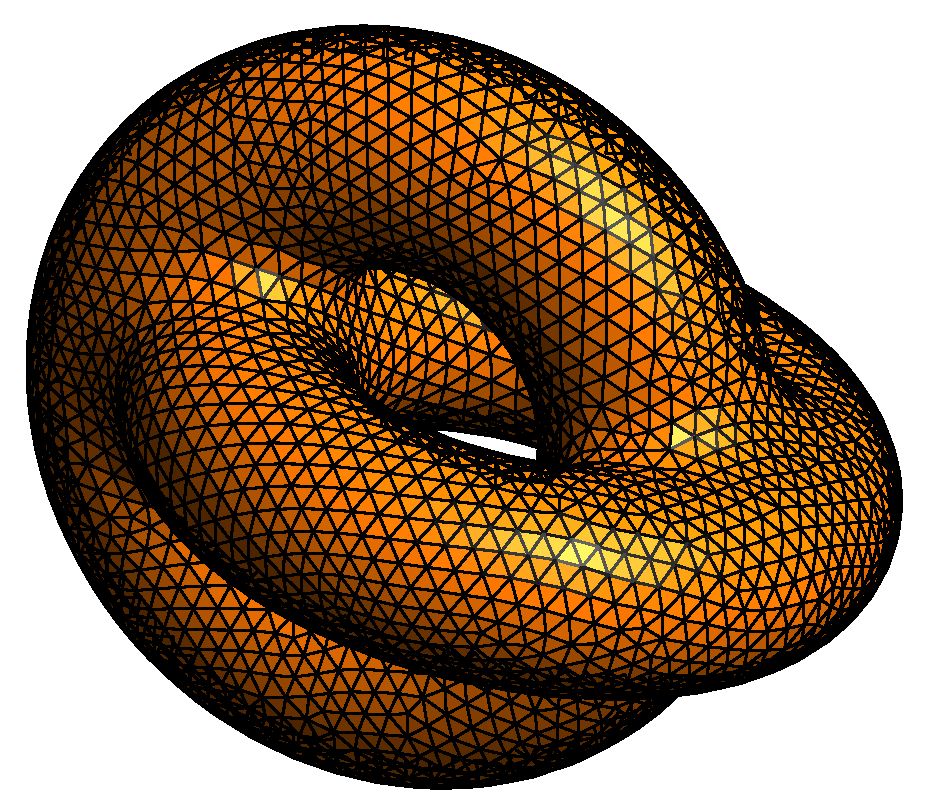
\includegraphics[width=90mm]{two-tori}
  \caption{Convolution between two tori}
\end{figure}

\begin{Verbatim}[commandchars=\\\{\},formatcom=\small\tt,frame=single,
   label=parag-\ref{\numb section 3.\numb parag 7}.cpp,rulecolor=\color{moldura},
   baselinestretch=0.94,framesep=2mm                                            ]
   \verm{Manifold} \azul{RR3} ( \textcolor{tag}{tag}::Euclid, \textcolor{tag}{tag}::of_dim, \laranja{3} );
   \verm{Function} \azul{xyz} = RR3 .build_coordinate_system ( \textcolor{tag}{tag}::Lagrange, \textcolor{tag}{tag}::of_degree, \laranja{1} );
   \verm{Function} \azul{x} = xyz [\laranja{0}], \azul{y} = xyz [\laranja{1}], \azul{z} = xyz [\laranja{2}];

   \verm{Function} \azul{f1} = \verm{max} ( x*x + y*y, \laranja{0.1} );  \cinza{// we cut by 0.1 to avoid singularities}
   \verm{Function} \azul{f2} = \laranja{1.} - \verm{power} ( f1, \laranja{-0.5} );
   \verm{Function} \azul{d1} = z*z + f1 * f2 * f2;  \cinza{// squared distance to a circle in the xy plane}
   \verm{Function} \azul{f3} = \verm{max} (x-\laranja{0.4})*(x-\laranja{0.4}) + z*z, \laranja{0.1} );
   \verm{Function} \azul{f4} = \laranja{1.} - \verm{power} ( f3, \laranja{-0.5} );
   \verm{Function} \azul{d2} = y*y + f3 * f4 *f4;  \cinza{// squared distance to a circle in the xz plane}

   \verm{Manifold} \azul{tori_manif} = RR3 .implicit
      ( \verm{smooth_min} ( d1, d2, \textcolor{tag}{tag}::threshold, \laranja{0.2} ) == \laranja{0.15} );

   \verm{Mesh} \azul{tori} ( \textcolor{tag}{tag}::frontal, \textcolor{tag}{tag}::desired_length, \laranja{0.09} );
\end{Verbatim}

Function {\small\tt\verm{smooth\_\,min}} gives a smooth approximation of the minimum between
two or more {\small\tt\verm{Function}} objects.
It is equal to the true minimum if the difference between the two values is higher, in
absolute value, than the provided threshold.
When the difference is smaller than the threshold, it gives a $ C^1 $ interpolation between
the two values.

If we want sharp edges, we must build the edges first as explained in paragraphs
\ref{\numb section 3.\numb parag 18} and \ref{\numb section 3.\numb parag 19}.

Comments at the end of paragraph \ref{\numb section 3.\numb parag 6} apply here, too :
{\maniFEM} must find a starting point and the right orientation.


\section{~~\cinzasec{[empty]}}\label{\numb section 3.\numb parag 8}


          %------------------%
\section{~~A bumpy hemisphere}\label{\numb section 3.\numb parag 9}
          %------------------%

We now look again at the surface in paragraph \ref{\numb section 2.\numb parag 17}
and build it with frontal meshing, using fewer lines of code.

\begin{Verbatim}[commandchars=\\\{\},formatcom=\small\tt,frame=single,
   label=parag-\ref{\numb section 3.\numb parag 9}.cpp,rulecolor=\color{moldura},
   baselinestretch=0.94,framesep=2mm                                            ]
   \verm{Manifold} \azul{nut} = RR3 .implicit ( x*x + y*y + z*z + \laranja{1.5}*x*y*z == \laranja{1.} );
   \verm{Manifold} \azul{base} = nut .implicit ( x*x + \laranja{3.}*z == \laranja{0.} );
   \verm{Mesh} \azul{circle}  \cinza{// 'base' is used by default as working manifold}
      ( \textcolor{tag}{tag}::frontal, \textcolor{tag}{tag}::desired_length, \laranja{0.1}, \textcolor{tag}{tag}::orientation, \textcolor{tag}{tag}::random );
   
   nut .set_as_working_manifold();
   \verm{Mesh} \azul{bumpy}  \cinza{// 'nut' is used as working manifold}
      ( \textcolor{tag}{tag}::frontal, \textcolor{tag}{tag}::boundary, circle, \textcolor{tag}{tag}::desired_length, \laranja{0.1} );
\end{Verbatim}

In this example, the issue of the orientation can be really tricky.
An orientation of the {\small\tt circle} is chosen at random.
As a consequence of this random choice, {\maniFEM} will unpredictably mesh the upper or
the lower hemisphere.
Paragraphs \ref{\numb section 3.\numb parag 10}, \ref{\numb section 3.\numb parag 13} and
\ref{\numb section 3.\numb parag 14} give more details.


          %-----------------------------%
\section{~~How the orientation is chosen}\label{\numb section 3.\numb parag 10}
          %-----------------------------%

In \maniFEM, cells and meshes are oriented (paragraphs \ref{\numb section 1.\numb parag 2}
and \ref{\numb section 9.\numb parag 5} provide details).
For building a mesh with frontal method, {\maniFEM} needs to know which orientation we want.

Manifolds may be oriented or not.
Euclidian manifolds (that is, the space $ \mathbb{R}^n $) have an intrinsic orientation,
given by the natural order of the $n$ coordinates.
Parametric manifolds inherit the intrinsic orientation from the space of parameters.
Implicit manifolds, however, have no intrinsic orientation.
We can specify an orientation of a manifold by attaching an outer form to it
(this feature is not implemented yet); otherwise, it will be considered not oriented.

In the example in paragraph \ref{\numb section 3.\numb parag 1}, the boundary {\small\tt circle}
is oriented according to the four segments composing it, {\small\tt NW}, {\small\tt WS},
{\small\tt SE} and {\small\tt EN}.
\ {\ManiFEM} uses the intrinsic orientation of the surrounding space {\small\tt RR2} in order
to determine the desired orientation of the mesh {\small\tt disk}.
The orientation of the boundary {\small\tt circle} is important;
together with the intrinsic orientation of the surrounding space,
it determines on which side of the circle the mesh will be propagated.
Had we built the segments {\small\tt NW}, {\small\tt WS}, {\small\tt SE} and {\small\tt EN} in the
opposite direction (that is, {\small\tt WN}, {\small\tt SW}, {\small\tt ES} and {\small\tt NE})
the program would try to mesh the exterior of the disk, never stopping.

Compact manifolds of co-dimension one (closed curves in $ \mathbb{R}^2 $,
compact surfaces in $ \mathbb{R}^3 $) are an exception among implicit manifolds.
Recall that in this manual we use the term ``manifold'' to mean a manifold without boundary.
There is a ``privileged'' orientation of a compact manifold of co-dimension one,
which is compatible with the intrinsic orientation of the surrounding space.
We call this orientation {\small\tt inherent}; paragraph \ref{\numb section 3.\numb parag 13}
discusses this topic.

Open curves (like the {\small\tt\azul{spiral}} in paragraphs \ref{\numb section 3.\numb parag 5} and
\ref{\numb section 3.\numb parag 12}), as well as non-compact manifolds
(like the {\small\tt\azul{cylinder}} in paragraphs \ref{\numb section 3.\numb parag 18} and
\ref{\numb section 3.\numb parag 19}), have no privileged orientation.
If we don't specify an orientation, these manifolds are considered not oriented.
If we don't specify a starting direction, {\maniFEM} will perform a preliminary search
in both directions and choose the one that first meets the stopping point.

Curves in $ \mathbb{R}^3 $, either closed like the {\small\tt circle} in paragraphs
\ref{\numb section 3.\numb parag 4} and \ref{\numb section 3.\numb parag 9} or open,
have no privileged orientation either (because they have co-dimension two).
There is no way to decide which of its two possible orientations
should be chosen; no one is more ``correct'' than the other.
This is why {\maniFEM} will reject a tentative to define {\small\tt\azul{circle}} without
{\small\tt\textcolor{tag}{tag}::orientation,} {\small\tt\textcolor{tag}{tag}::random}
as last arguments to the {\small\tt\verm{Mesh}} constructor.
A statement like {\small\tt\verm{Mesh}} {\small\tt circle} {\small\tt (}
{\small\tt\textcolor{tag}{tag}::frontal,} {\small\tt\textcolor{tag}{tag}::desired\_\,length,}
some\_\,value {\small\tt)}
will produce a run-time error if the current working manifold has dimension 1 and
the geometric dimension (that is, the number of coordinates) is 3.

The options given to the constructor of {\small\tt\verm{Mesh}}es {\small\tt\azul{circle}} and
{\small\tt\azul{bumpy}} in paragraph \ref{\numb section 3.\numb parag 9} are discussed in paragraph
\ref{\numb section 3.\numb parag 14}.


\section{~~\cinzasec{[empty]}}\label{\numb section 3.\numb parag 11}


          %------------------------%
\section{~~Specifying the direction}\label{\numb section 3.\numb parag 12}
          %------------------------%

For one-dimensional manifolds, we can specify, along with the starting point,
a starting direction, thus saving some computational time.
The code producing the spiral in paragraph \ref{\numb section 3.\numb parag 5}
can be changed as below.

\begin{Verbatim}[commandchars=\\\{\},formatcom=\small\tt,
   baselinestretch=0.94,framesep=2mm                     ]
   \verm{Cell} \azul{A} ( \textcolor{tag}{tag}::vertex );  x (A) =    pi*pi;  y (A) = \laranja{0.};
   \verm{Cell} \azul{B} ( \textcolor{tag}{tag}::vertex );  x (B) = \laranja{81}*pi*pi;  y (B) = \laranja{0.};
   std::vector < double > \azul{direc} = \{ \laranja{0.}, \laranja{1.} \};
   \verm{Mesh} \azul{spiral} ( \textcolor{tag}{tag}::frontal, \textcolor{tag}{tag}::start_at, A, \textcolor{tag}{tag}::towards, direc,
                 \textcolor{tag}{tag}::stop_at, B, \textcolor{tag}{tag}::desired_length, \laranja{1.}            );
\end{Verbatim}

Note that the vector {\small\tt direc} is associated to the point {\small\tt A}
(is tangent to the manifold at point {\small\tt A}).

Recall that open curves have no ``default'' (or ``inherent'') orientation.
{\ManiFEM} uses the vector {\small\tt direc} as an indication about where to go.

It is the user's responsibility to ensure that, going in the specified direction,
the algorithm will eventually meet the stopping point {\small\tt B}.
Otherwise, we may end up spinning endlessly along the spiral.

We could specify in a similar fashion the orientation of {\small\tt circle} in paragraph
\ref{\numb section 3.\numb parag 2}, thus saving some computational time :

\begin{Verbatim}[commandchars=\\\{\},formatcom=\small\tt,
   baselinestretch=0.94,framesep=2mm                     ]
   \verm{Cell} \azul{A} ( \textcolor{tag}{tag}::vertex );  x (A) = \laranja{1.};  y (A) = \laranja{0.};
   \verm{Mesh} \azul{circle} ( \textcolor{tag}{tag}::frontal, \textcolor{tag}{tag}::start_at, A,
                 \textcolor{tag}{tag}::towards, \{ \laranja{0.}, \laranja{1.} \}, \textcolor{tag}{tag}::desired_length, \laranja{0.2} );
\end{Verbatim}

If, in the above, we choose the opposite {\small\tt direc}tion,
{\maniFEM} will later try to mesh the exterior of the disk.

The same technique can be used for building the {\small\tt circle} in paragraph
\ref{\numb section 3.\numb parag 4}, thus avoiding \maniFEM's random choice of the orientation :

\begin{Verbatim}[commandchars=\\\{\},formatcom=\small\tt,
   baselinestretch=0.94,framesep=2mm                     ]
   \verm{Cell} \azul{S} ( \textcolor{tag}{tag}::vertex );  x (S) = \laranja{0.};  y (S) = \laranja{-1.};  z (S) = \laranja{0.};
   \verm{Manifold} \azul{circle_manif} = RR3 .implicit ( x*x + y*y == \laranja{1.}, x*y == \laranja{4.}*z );
   \verm{Mesh} \azul{circle} ( \textcolor{tag}{tag}::frontal, \textcolor{tag}{tag}::start_at, S,
                 \textcolor{tag}{tag}::towards, \{ \laranja{1.}, \laranja{0.}, \laranja{0.} \}, \textcolor{tag}{tag}::desired_length, \laranja{0.2} );
\end{Verbatim}

This also applies to the example in paragraph \ref{\numb section 3.\numb parag 9}.
However, there the topologic considerations are more complex, so we delegate this
discussion to paragraph \ref{\numb section 3.\numb parag 14}.


          %---------------------------------------%
\section{~~The intrinsic and inherent orientations}\label{\numb section 3.\numb parag 13}
          %---------------------------------------%

Euclidian manifolds have an intrinsic orientation given by the natural order of the
coordinates.
{\ManiFEM} will always use this orientation when the working manifold is Euclidian.
We can enforce the requirement of using the intrinsic orientation by providing
{\small\tt\textcolor{tag}{tag}::orientation,} {\small\tt\textcolor{tag}{tag}::intrinsic}
as arguments to the {\small\tt\verm{Mesh}} constructor.
However, these arguments are not necessary; {\maniFEM} will consider them by default.
This happens for the {\small\tt\azul{disk}} in paragraphs \ref{\numb section 3.\numb parag 1} and
\ref{\numb section 3.\numb parag 2}, for the diamond in
paragraph \ref{\numb section 3.\numb parag 17} and for the annulus in paragraphs
\ref{\numb section 3.\numb parag 3}, \ref{\numb section 3.\numb parag 22}
and \ref{\numb section 3.\numb parag 24}.

Compact manifolds of co-dimension one (closed curves in $ \mathbb{R}^2 $,
compact surfaces in $ \mathbb{R}^3 $) have a privileged orientation,
compatible with the intrinsic orientation of the surrounding space;
we call this orientation ``inherent''.
Such a manifold cuts the surrounding space in two regions, one of them being bounded;
the ``inherent'' orientation is the one pointing towards the unbounded region;
intuitively speaking, it points ``outwards''.
{\ManiFEM} will choose it in some situations, unless we provide
{\small\tt\textcolor{tag}{tag}::orientation,} {\small\tt\textcolor{tag}{tag}::random}
as arguments to the {\small\tt\verm{Mesh}} constructor.
We can enforce the requirement of finding the inherent orientation by providing
{\small\tt\textcolor{tag}{tag}::orientation,} {\small\tt\textcolor{tag}{tag}::inherent}
as arguments to the {\small\tt\verm{Mesh}} constructor;
however, {\maniFEM} will consider these arguments by default when we provide no stopping
point (for one-dimensional meshes) or we provide no boundary (for two-dimensional meshes).
In these cases, {\maniFEM} will assume that the manifold is compact and, if it has
co-dimension one, the inherent orientation will be used.
This happens for the {\small\tt\azul{circle}} in paragraph \ref{\numb section 3.\numb parag 2},
for the {\small\tt\azul{sphere}} in paragraph \ref{\numb section 3.\numb parag 6} and for the
{\small\tt\azul{tori}} in paragraph \ref{\numb section 3.\numb parag 7}.

If we do provide a stopping point, or a boundary, {\maniFEM} has no means to know in
advance whether the manifold
is compact or not, so it will not try to find the inherent orientation.
This happens for the {\small\tt\azul{spiral}} and for the {\small\tt\azul{arc\_\,of\_\,circle}}
in paragraph \ref{\numb section 3.\numb parag 5}, for the {\small\tt\azul{bumpy}} hemisphere
in paragraph \ref{\numb section 3.\numb parag 9}, for the {\small\tt\azul{piece\_\,of\_\,cyl}} and
{\small\tt\azul{piece\_\,of\_\,sph}} in paragraphs \ref{\numb section 3.\numb parag 18} and
\ref{\numb section 3.\numb parag 19} and others.
In these situations, we may require specifically the inherent orientation
by providing the {\small\tt\textcolor{tag}{tag}::orientation,}
{\small\tt\textcolor{tag}{tag}::inherent} arguments to the {\small\tt\verm{Mesh}} constructor.
Do not misuse this option; if you ask {\maniFEM} to find the inherent orientation of an open
curve or of a non-compact surface, it will not complain but will hopelessly try to mesh
the entire manifold, never stopping.
For instance, in paragraph \ref{\numb section 3.\numb parag 5} it makes sense to enforce the
inherent orientation for the {\small\tt\azul{arc\_\,of\_\,circle}} but not for the
{\small\tt\azul{spiral}}.
Also, in paragraphs \ref{\numb section 3.\numb parag 18} and
\ref{\numb section 3.\numb parag 19} it makes sense to enforce the inherent orientation
for the {\small\tt\azul{piece\_\,of\_\,sph}} but not for the {\small\tt\azul{piece\_\,of\_\,cyl}}.

Determining the intrinsic orientation of a Euclidian manifold is computationally
very cheap.
However, determining the inherent orientation of a manifold of co-dimension one is not
a trivial computational process.
{\ManiFEM} is unable to determine this orientation by looking at the equations defining
the manifold; it needs a mesh on the entire manifold.

So, in paragraph \ref{\numb section 3.\numb parag 2} we obtain a correctly oriented mesh
on the disk, with no need to provide any specific information about the orientation of
{\small\tt circle\_\,manif}.
Behind the curtains, {\maniFEM} builds a mesh on {\small\tt circle\_\,manif} with
an initially arbitrary orientation, then checks its consistency
within the surrounding manifold and, if necessary, switches the orientation of the produced mesh.
Later, when we ask {\maniFEM} to mesh the {\small\tt\azul{disk}}, the orientation of the boundary
(together with the intrinsic orientation of the surrounding space {\small\tt RR2})
defines whether the interior or the exterior of the disk is to be meshed.

A similar process happens for compact surfaces in $ \mathbb{R}^3 $ like those
considered in paragraphs \ref{\numb section 3.\numb parag 6} and
\ref{\numb section 3.\numb parag 7},
except that checking the orientation of a compact surface has a computational cost
considerably higher than for a closed curve in $ \mathbb{R}^2 $.

You can save some computing time if you specify the orientation
yourself, either by providing more information to the {\small\tt\verm{Mesh}} constructor as shown
in paragraph \ref{\numb section 3.\numb parag 15} or by attaching this information to
the manifold itself (this feature is not implemented yet).
% in order to alleviate the computational burden
 
If the orientation is not important for you, you can add to the {\small\tt\verm{Mesh}} constructor
the arguments {\small\tt\textcolor{tag}{tag}::orientation,}
{\small\tt\textcolor{tag}{tag}::random} and {\maniFEM} will not waste
computing time to find the inherent orientation.


          %-------------------------------%
\section{~~Revisiting the bumpy hemisphere}\label{\numb section 3.\numb parag 14}
          %-------------------------------%

%The random behaviour in this example is quite dramatic.
Let us have a closer look at the code in paragraph \ref{\numb section 3.\numb parag 9}.
The manifold {\small\tt nut} has a unique orientation consistent with the surrounding
space, just like those in paragraphs \ref{\numb section 3.\numb parag 6} and
\ref{\numb section 3.\numb parag 7}, but the {\small\tt base} within it has not.
This is why, when we build the {\small\tt circle}, we must provide
{\small\tt\textcolor{tag}{tag}::orientation,} {\small\tt\textcolor{tag}{tag}::random}
as last arguments to the {\small\tt\verm{Mesh}} constructor,
or specify the orientation by providing a starting point and a starting direction
as described in paragraph \ref{\numb section 3.\numb parag 12}.

When we build {\small\tt bumpy}, since we are providing a boundary, {\maniFEM} does not treat
the current working manifold {\small\tt nut} as compact, that is, it does not try to determine an
inherent orientation.
It will start the meshing process on an arbitrary side of {\small\tt circle}, thus meshing
unpredictably the upper or the lower {\small\tt bumpy} hemisphere.

If we enforce the orientation by providing
{\small\tt\textcolor{tag}{tag}::orientation,} {\small\tt\textcolor{tag}{tag}::inherent} as last
arguments to the {\small\tt\verm{Mesh}} constructor of {\small\tt bumpy},
then {\maniFEM} will mesh (behind the curtains) both halves of the sphere;
let's call them {\small\tt msh1} and {\small\tt msh2}.
Note that the {\small\tt circle} has already been built, so its orientation is given.
Both {\small\tt msh1} and {\small\tt msh2} have {\small\tt circle} as boundary,
which means that they have mutually incompatible orientations.
They cannot be {\small\tt join}ed.
But the reverse of any of them can be {\small\tt join}ed with the other one, the result being a
mesh on the entire bumpy sphere.
Two choices are possible : either {\small\tt msh1.reverse()} is {\small\tt join}ed with
{\small\tt msh2} or {\small\tt msh1} is {\small\tt join}ed with {\small\tt msh2.reverse()},
resulting in two meshes on the same compact surface with opposite orientations.
One of these orientations is compatible with the intrinsic orientation of the surrounding space
$ \mathbb{R}^3 $ and is called inherent orientation.
If the first one is correctly oriented, {\small\tt msh2} will be returned;
if the second one is correctly oriented, {\small\tt msh1} will be returned.
\vfil\eject

Thus, in the code below we will obtain the upper hemisphere.

\begin{Verbatim}[commandchars=\\\{\},formatcom=\small\tt,
   baselinestretch=0.94,framesep=2mm                      ]
   \verm{Cell} \azul{S} ( \textcolor{tag}{tag}::vertex );  x (S) = \laranja{0.};  y (S) = \laranja{-1.};  z (S) = \laranja{0.};
   \verm{Mesh} \azul{circle} ( \textcolor{tag}{tag}::frontal, \textcolor{tag}{tag}::start_at, S, \textcolor{tag}{tag}::towards, \{ \laranja{1.}, \laranja{0.}, \laranja{0.} \},
                 \textcolor{tag}{tag}::desired_length, \laranja{0.1}                                     );
   nut .set_as_working_manifold();
   \verm{Mesh} \azul{bumpy} ( \textcolor{tag}{tag}::frontal, \textcolor{tag}{tag}::boundary, circle,
                \textcolor{tag}{tag}::desired_length, \laranja{0.1}, \textcolor{tag}{tag}::orientation, \textcolor{tag}{tag}::inherent );
\end{Verbatim}

Code below will produce the lower hemisphere.

\begin{Verbatim}[commandchars=\\\{\},formatcom=\small\tt,
   baselinestretch=0.94,framesep=2mm                      ]
   \verm{Cell} \azul{S} ( \textcolor{tag}{tag}::vertex );  x (S) = \laranja{0.};  y (S) = \laranja{-1.};  z (S) = \laranja{0.};
   \verm{Mesh} \azul{circle} ( \textcolor{tag}{tag}::frontal, \textcolor{tag}{tag}::start_at, S, \textcolor{tag}{tag}::towards, \{ \laranja{-1.},\laranja{ 0.}, \laranja{0.} \},
                 \textcolor{tag}{tag}::desired_length, \laranja{0.1}                                      );
   nut .set_as_working_manifold();
   \verm{Mesh} \azul{bumpy} ( \textcolor{tag}{tag}::frontal, \textcolor{tag}{tag}::boundary, circle,
                \textcolor{tag}{tag}::desired_length, \laranja{0.1}, \textcolor{tag}{tag}::orientation, \textcolor{tag}{tag}::inherent );
\end{Verbatim}

Code below will unpredictably mesh the upper or the lower hemisphere;
in either case, the produced mesh will be oriented upwards because the orientation
of {\small\tt circle} points upwards.
Here, the word ``upwards'' is used in the sense of the right hand rule
(see paragraph \ref{\numb section 1.\numb parag 2}).

\begin{Verbatim}[commandchars=\\\{\},formatcom=\small\tt,
   baselinestretch=0.94,framesep=2mm                     ]
   \verm{Cell} \azul{S} ( \textcolor{tag}{tag}::vertex );  x (S) = \laranja{0.};  y (S) = \laranja{-1.};  z (S) = \laranja{0.};
   \verm{Mesh} \azul{circle} ( \textcolor{tag}{tag}::frontal, \textcolor{tag}{tag}::start_at, S, \textcolor{tag}{tag}::towards, \{ \laranja{1.}, \laranja{0.}, \laranja{0.} \},
                 \textcolor{tag}{tag}::desired_length, \laranja{0.1}                                     );
   nut .set_as_working_manifold();
   \verm{Mesh} \azul{bumpy} ( \textcolor{tag}{tag}::frontal, \textcolor{tag}{tag}::boundary, circle, \textcolor{tag}{tag}::desired_length, \laranja{0.1} );
\end{Verbatim}

Code below will unpredictably mesh the upper or the lower hemisphere;
in either case, the produced mesh will be oriented downwards.

\begin{Verbatim}[commandchars=\\\{\},formatcom=\small\tt,
   baselinestretch=0.94,framesep=2mm                     ]
   \verm{Cell} \azul{S} ( \textcolor{tag}{tag}::vertex );  x (S) = \laranja{0.};  y (S) = \laranja{-1.};  z (S) = \laranja{0.};
   \verm{Mesh} \azul{circle} ( \textcolor{tag}{tag}::frontal, \textcolor{tag}{tag}::start_at, S, \textcolor{tag}{tag}::towards, \{ \laranja{-1.}, \laranja{0.}, \laranja{0.} \},
                 \textcolor{tag}{tag}::desired_length, \laranja{0.1}                                      );
   nut .set_as_working_manifold();
   \verm{Mesh} \azul{bumpy} ( \textcolor{tag}{tag}::frontal, \textcolor{tag}{tag}::boundary, circle, \textcolor{tag}{tag}::desired_length, \laranja{0.1} );
\end{Verbatim}

Code below will still mesh unpredictably either the upper or the lower
hemisphere, but only due to the random choice in the orientation of {\small\tt circle}.
The construction of {\small\tt bumpy} is uniquely determined by the orientation of
{\small\tt circle}.

\begin{Verbatim}[commandchars=\\\{\},formatcom=\small\tt,
   baselinestretch=0.94,framesep=2mm                      ]
   \verm{Manifold} \azul{nut} = RR3.implicit ( x*x + y*y + z*z + \laranja{1.5}*x*y*z == \laranja{1.} );
   \verm{Manifold} \azul{base} = nut.implicit ( x*x + 3.*z == 0. );
   \verm{Mesh} \azul{circle}
      ( \textcolor{tag}{tag}::frontal, \textcolor{tag}{tag}::desired_length, \laranja{0.1}, \textcolor{tag}{tag}::orientation, \textcolor{tag}{tag}::random );
   nut .set_as_working_manifold();
   \verm{Mesh} \azul{bumpy} ( \textcolor{tag}{tag}::frontal, \textcolor{tag}{tag}::boundary, circle,
                \textcolor{tag}{tag}::desired_length, \laranja{0.1}, \textcolor{tag}{tag}::orientation, \textcolor{tag}{tag}::inherent );
\end{Verbatim}


          %------------------------%
\section{~~Specifying the direction}\label{\numb section 3.\numb parag 15}
          %------------------------%

In paragraph \ref{\numb section 3.\numb parag 12} we have seen how we can specify the direction
of propagation of the mesh for one-dimensional manifolds.
A similar approach can be taken for two-dimensional meshes.
For instance, code below will mesh the upper half of the ``bumpy hemisphere'' already considered
in paragraphs \ref{\numb section 2.\numb parag 17}, \ref{\numb section 3.\numb parag 9} and
\ref{\numb section 3.\numb parag 14}, oriented upwards.

\begin{Verbatim}[commandchars=\\\{\},formatcom=\small\tt,frame=single,
   label=parag-\ref{\numb section 3.\numb parag 15}.cpp,rulecolor=\color{moldura},
   baselinestretch=0.94,framesep=2mm                                            ]
   \verm{Cell} \azul{S} ( \textcolor{tag}{tag}::vertex );  x (S) = \laranja{0.};  y (S) = \laranja{-1.};  z (S) = \laranja{0.};
   std::vector < double > \azul{tau} \{ \laranja{1.}, \laranja{0.}, \laranja{0.} \};
   \verm{Mesh} \azul{circle} ( \textcolor{tag}{tag}::frontal, \textcolor{tag}{tag}::start_at, S, \textcolor{tag}{tag}::towards, tau,
                 \textcolor{tag}{tag}::desired_length, \laranja{0.1}                          );
   nut .set_as_working_manifold();
   std::vector < double > \azul{N} \{ \laranja{0.}, \laranja{0.}, \laranja{1.} \};
   \verm{Mesh} bumpy ( \textcolor{tag}{tag}::frontal, \textcolor{tag}{tag}::boundary, circle,
                \textcolor{tag}{tag}::start_at, S, \textcolor{tag}{tag}::towards, N,
                \textcolor{tag}{tag}::desired_length, \laranja{0.1}            );
\end{Verbatim}

If we define {\small\tt\azul N} as \catcode`<=1\catcode`>=2\catcode`{=12\catcode`}=12<\small\tt {>
<\small\tt\laranja0\laranja.,> <\small\tt\laranja0\laranja.,>
<\small\tt \laranja-\laranja1\laranja.> <\small\tt }>\catcode`<=12\catcode`>=12\catcode`{=1\catcode`}=2, we will obtain
the lower half of the ``sphere'', still oriented upwards.

If we define {\small\tt\azul{tau}} as \catcode`<=1\catcode`>=2\catcode`{=12\catcode`}=12<\small\tt {>
<\small\tt\laranja-\laranja1\laranja.,> <\small\tt\laranja0\laranja.,> <\small\tt\laranja0\laranja.> <\small\tt }>\catcode`<=12\catcode`>=12\catcode`{=1\catcode`}=2, we will get a mesh
oriented downwards.


          %---------------------%
\section{~~Geometric limitations}\label{\numb section 3.\numb parag 16}
          %---------------------%

Frontal meshing has its limits.
{\ManiFEM} cannot mesh a manifold whose curvature is too high when compared to the
length of the segments.
The example in paragraph \ref{\numb section 3.\numb parag 7} is ``on the edge'', that is,
if we increase the segment size the meshing process will probably get stuck somewhere.

Also, we should avoid domains whose boundary has components too close to each other,
when compared to the segment size.
In this respect, the example in paragraph \ref{\numb section 3.\numb parag 3} is also
``on the edge''.
In contrast, {\maniFEM} is ``at ease'' when meshing the same domain with other options,
like in paragraphs \ref{\numb section 3.\numb parag 22}, \ref{\numb section 3.\numb parag 23}
or \ref{\numb section 3.\numb parag 24}.

Sharp edges and singularities must be dealt with as described in subsequent paragraphs.

The example in paragraph \ref{\numb section 3.\numb parag 1} is also ``on the edge''
for a different reason.
While {\maniFEM} tries to build a mesh with segments of constant given length,
the length of the segments on the boundary of the disk varies (paragraphs
\ref{\numb section 2.\numb parag 4} and \ref{\numb section 2.\numb parag 5} explain why).
This contradiction puts the algorithm in a difficult position.
If the variation were larger (or sharper) the algorithm might stop with some error message.
In contrast, {\maniFEM} is ``at ease'' when meshing the disk in paragraph
\ref{\numb section 3.\numb parag 2} because there the segments on the boundary have
(approximately) constant length.

This is a good place to mention that \maniFEM's frontal meshing algorithm is still not
as robust as we would like it to be.
In rare occasions, it reports as ``unmanageable'' certain geometric configurations which
should be manageable.
A fresh implementation is on its way.


          %------------%
\section{~~Sharp angles}\label{\numb section 3.\numb parag 17}
          %------------%

{\ManiFEM} can deal with non-smooth domains.
The user must define separately smooth pieces of the boundary and then join them.

Here is how to mesh the diamond-shaped domain in paragraph \ref{\numb section 2.\numb parag 11}.

\begin{Verbatim}[commandchars=\\\{\},formatcom=\small\tt,frame=single,
   label=parag-\ref{\numb section 3.\numb parag 17}.cpp,rulecolor=\color{moldura},
   baselinestretch=0.94,framesep=2mm                                            ]
   \cinza{// we define the arcs NW, WS, SE and EN either as segments, like in}
   RR2 .implicit ( x*y + x - y == \laranja{-1.} );
   \verm{Mesh} \azul{NW} ( \textcolor{tag}{tag}::segment, N .reverse(), W, \textcolor{tag}{tag}::divided_in, \laranja{12} );
   
   \cinza{// or with tag::frontal like in}
   RR2 .implicit ( x*y - x - y ==  \laranja{1.} );
   \verm{Mesh} \azul{WS} ( \textcolor{tag}{tag}::frontal, \textcolor{tag}{tag}::start_at, W, \textcolor{tag}{tag}::stop_at, S,
             \textcolor{tag}{tag}::desired_length, \laranja{0.1}                        );
   \cinza{// ... //}
             
   \verm{Mesh} \azul{bdry} ( \textcolor{tag}{tag}::join, NW, WS, SE, EN );
   RR2 .set_as_working_manifold();
   \verm{Mesh} \azul{diamond} ( \textcolor{tag}{tag}::frontal, \textcolor{tag}{tag}::boundary, bdry, \textcolor{tag}{tag}::desired_length, \laranja{0.1} );
\end{Verbatim}


          %-----------%
\section{~~Sharp edges}\label{\numb section 3.\numb parag 18}
          %-----------%

We can mesh surfaces with sharp edges, by building individually smooth pieces of surface
and then {\small\tt join}ing them.
The edges must be built first;
thus, some previous knowledge about the geometry of the surface is needed.

\begin{figure}[ht] \centering
 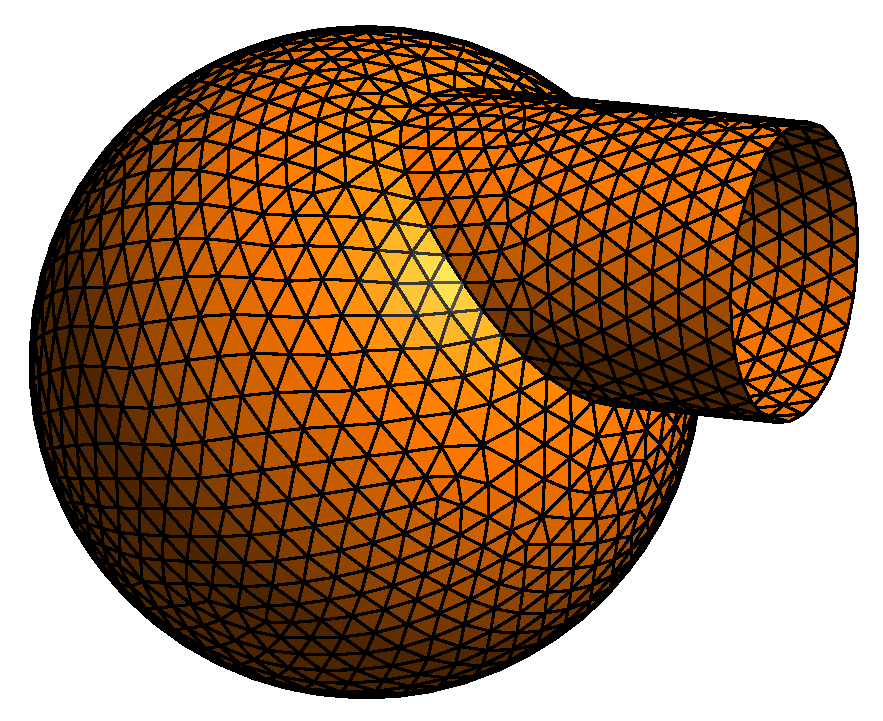
\includegraphics[width=94mm]{sphere-cyl}
  \caption{Sphere glued to cylinder}
  \label{\numb section 3.\numb fig 5}
\end{figure}

\begin{Verbatim}[commandchars=\\\{\},formatcom=\small\tt,frame=single,
   label=parag-\ref{\numb section 3.\numb parag 18}.cpp,rulecolor=\color{moldura},
   baselinestretch=0.94,framesep=2mm                                            ]
   \verm{Manifold} \azul{RR3} ( \textcolor{tag}{tag}::Euclid, \textcolor{tag}{tag}::of_dim, \laranja{3} );
   \verm{Function} \azul{xyz} = RR3 .build_coordinate_system ( \textcolor{tag}{tag}::Lagrange, \textcolor{tag}{tag}::of_degree, \laranja{1} );
   \verm{Function} \azul{x} = xyz [\laranja{0}], \azul{y} = xyz [\laranja{1}], \azul{z} = xyz [\laranja{2}];

   const double \azul{rs} = \laranja{1.};    \cinza{// radius of the sphere}
   const double \azul{rc} = \laranja{0.45};  \cinza{// radius of the cylinder}
   const double seg_size = \laranja{0.1};

   \verm{Manifold} \azul{cylinder} = RR3 .implicit ( y*y + (z-\laranja{0.5})*(z-\laranja{0.5}) == rc*rc );

   cylinder .implicit ( x == \laranja{1.5} );  \cinza{// we cut the cylinder on its right side}
   \verm{Cell} \azul{start_1} ( \textcolor{tag}{tag}::vertex );
   x ( start_1 ) = \laranja{1.5};  y ( start_1 ) = \laranja{0.};  z ( start_1 ) = \laranja{0.5} + rc;
   \verm{Mesh} \azul{circle_1} ( \textcolor{tag}{tag}::frontal, \textcolor{tag}{tag}::start_at, start_1,
                   \textcolor{tag}{tag}::towards, \{ \laranja{0.}, \laranja{1.}, \laranja{0.} \}, \textcolor{tag}{tag}::desired_length, seg_size );

   \cinza{// we cut the cylinder on its left side with a sphere}
   \verm{Manifold} \azul{intersection} = cylinder .implicit ( x*x + y*y + z*z == rs*rs );
   \verm{Cell} \azul{start_2} ( \textcolor{tag}{tag}::vertex );
   x ( start_2 ) = \laranja{1.};  y ( start_2 ) = \laranja{0.};  z ( start_2 ) = \laranja{0.5} - rc;
   intersection .project ( start_2 );
   \verm{Mesh} \azul{circle_2} ( \textcolor{tag}{tag}::frontal, \textcolor{tag}{tag}::start_at, start_2,
                   \textcolor{tag}{tag}::towards, \{ \laranja{0.}, \laranja{-1.}, \laranja{0.} \}, \textcolor{tag}{tag}::desired_length, seg_size );

   \verm{Mesh} \azul{two_circles} ( \textcolor{tag}{tag}::join, circle_1, circle_2 .reverse() );
   cylinder .set_as_working_manifold();
   \verm{Mesh} \azul{piece_of_cyl} ( \textcolor{tag}{tag}::frontal, \textcolor{tag}{tag}::boundary, two_circles,
                       \textcolor{tag}{tag}::start_at, start_1, \textcolor{tag}{tag}::towards, \{ \laranja{-1.}, \laranja{0.}, \laranja{0.} \},
                       \textcolor{tag}{tag}::desired_length, seg_size                         );
   RR3 .implicit ( x*x + y*y + z*z == rs*rs );
   \verm{Mesh} \azul{piece_of_sph} ( \textcolor{tag}{tag}::frontal, \textcolor{tag}{tag}::boundary, circle_2,
                       \textcolor{tag}{tag}::start_at, start_2, \textcolor{tag}{tag}::towards, \{ \laranja{0.}, \laranja{0.}, \laranja{-1.} \},
                       \textcolor{tag}{tag}::desired_length, seg_size                         );
                       
   \verm{Mesh} \azul{sphere_and_cylinder} ( \textcolor{tag}{tag}::join, piece_of_sph, piece_of_cyl );
\end{Verbatim}

Note how the orientation is important (see paragraphs \ref{\numb section 1.\numb parag 2}
and \ref{\numb section 1.\numb parag 4}).
For meshing the piece of cylinder, we provide its future boundary which is the union of
{\small\tt circle\_\,1} with {\small\tt circle\_\,2.reverse()}.
For meshing the sphere, we provide {\small\tt circle\_\,2}.
In figure \ref{\numb section 3.\numb fig 6}, where a crack has been opened artificially,
we see that the common boundary has a certain orientation when seen from the cylinder and
has the opposite orientation when seen from the sphere.
If we do not respect these orientations, {\maniFEM} will be unable to {\small\tt join} the two
meshes.

\begin{figure}[ht] \centering
 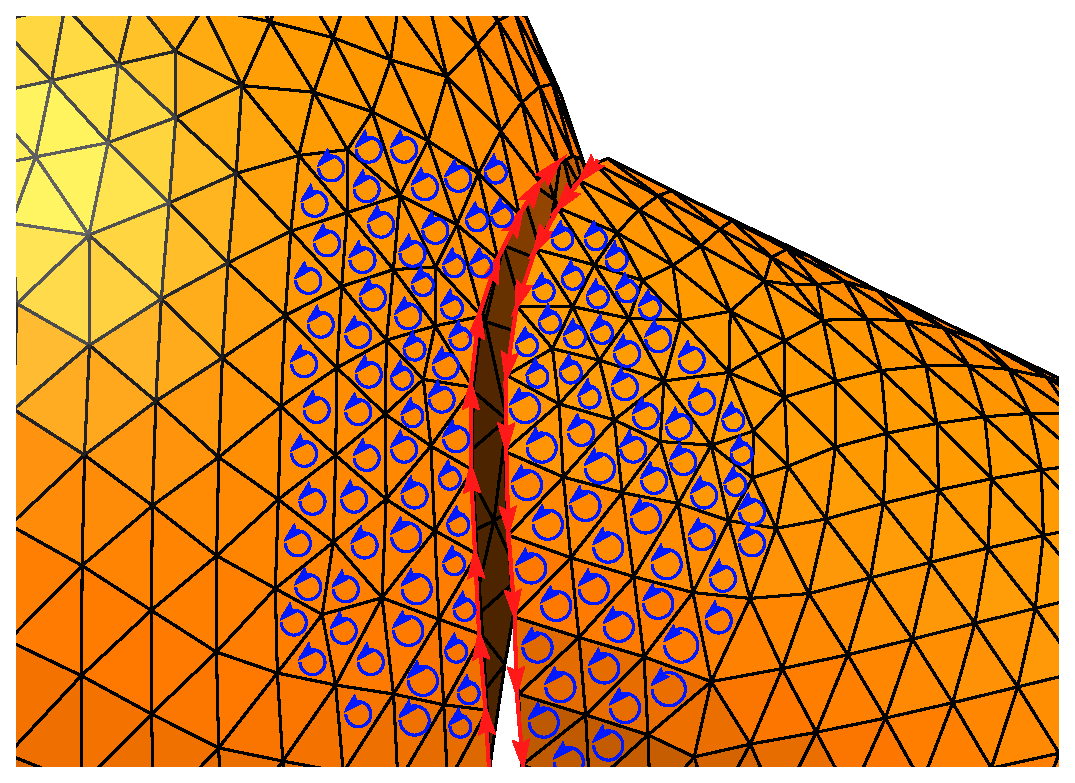
\includegraphics[width=100mm]{crack}
  \caption{Zoom around the joint}
  \label{\numb section 3.\numb fig 6}
\end{figure}

Note that {\small\tt intersection} is a disconnected manifold, made of two closed loops,
one of them being {\small\tt circle\_\,2} (the other one shows up in
paragraph \ref{\numb section 3.\numb parag 19} under the name {\small\tt circle\_\,3}).
We must provide detailed information to the {\small\tt\verm{Mesh}} constructor in order to
obtain the correct loop with the correct orientation.
A statement like

\begin{Verbatim}[commandchars=\\\{\},formatcom=\small\tt,
   baselinestretch=0.94,framesep=2mm                     ]
   \verm{Mesh} \azul{circle_2} ( \textcolor{tag}{tag}::frontal, \textcolor{tag}{tag}::desired_length, seg_size );
\end{Verbatim}

\noindent would produce a run-time error asking the user to specify the orientation
(see comments in paragraph \ref{\numb section 3.\numb parag 10} about curves in $ \mathbb{R}^3 $).
If we didn't care about the orientation (but we do care in this example), we could use
a constructor like

\begin{Verbatim}[commandchars=\\\{\},formatcom=\small\tt,
   baselinestretch=0.94,framesep=2mm                     ]
   \verm{Mesh} \azul{circle_2} ( \textcolor{tag}{tag}::frontal, \textcolor{tag}{tag}::desired_length, seg_size,
                   \textcolor{tag}{tag}::orientation, \textcolor{tag}{tag}::random               );
\end{Verbatim}

\noindent and {\maniFEM} would mesh one connected component of the manifold {\small\tt intersection}
(we would have no control on which component {\maniFEM} happens to find).

If we want to close the extremity of the cylinder, it suffices to add a few lines of code$\,$:

\begin{Verbatim}[commandchars=\\\{\},formatcom=\small\tt,
   baselinestretch=0.94,framesep=2mm                     ]
   RR3 .implicit ( x == \laranja{1.5} );
   \verm{Mesh} \azul{disk} ( \textcolor{tag}{tag}::frontal, \textcolor{tag}{tag}::boundary, circle_1 .reverse(),
               \textcolor{tag}{tag}::start_at, start_1, \textcolor{tag}{tag}::towards, \{ \laranja{0.}, \laranja{0.}, \laranja{-1.} \},
               \textcolor{tag}{tag}::desired_length, seg_size                         );
   \verm{Mesh} \azul{sphere_and_cylinder} ( \textcolor{tag}{tag}::join, piece_of_sph, piece_of_cyl, disk );
\end{Verbatim}

We have chosen the diameter of the cylinder slightly smaller than $1$.
Had we chosen a diameter equal to $1$, the cylinder would be tangent to the sphere at point
$ (0,0,1) $.
At that point, the two equations defining the {\small\tt intersection} manifold would be
degenerate (the Jacobian matrix would not have full rank).
This is a situation which {\maniFEM} cannot handle yet; it is discussed in paragraph
\ref{\numb section 3.\numb parag 21}.


          %------------------%
\section{~~Sharp edges, again}\label{\numb section 3.\numb parag 19}
          %------------------%

With a few changes to the code in paragraph \ref{\numb section 3.\numb parag 18},
we can cut two holes in the sphere and create a tunnel using the cylinder's wall.
\medskip

\begin{Verbatim}[commandchars=\\\{\},formatcom=\small\tt,frame=single,
   label=parag-\ref{\numb section 3.\numb parag 19}.cpp,rulecolor=\color{moldura},
   baselinestretch=0.94,framesep=2mm                                              ]
   \verm{Manifold} \azul{cylinder} = RR3 .implicit ( y*y + (z-\laranja{0.5})*(z-\laranja{0.5}) == rc*rc );

   \verm{Manifold} \azul{intersection} = cylinder .implicit ( x*x + y*y + z*z == rs*rs );

   \cinza{// we choose names start_2 and circle_2 for consistency with previous paragraph}
   \verm{Cell} \azul{start_2} ( \textcolor{tag}{tag}::vertex );
   x ( start_2 ) = \laranja{1.};  y ( start_2 ) = \laranja{0.};  z ( start_2 ) = \laranja{0.5} - rc;
   intersection .project ( start_2 );
\end{Verbatim}

\begin{figure}[ht] \centering
\if\production 1
 \includegraphics[width=85mm]{sphere-tunnel-cloud-im}
\else
 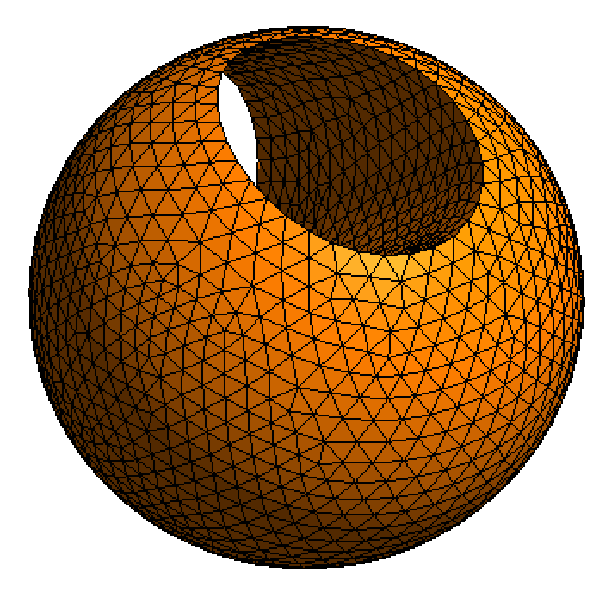
\includegraphics[width=85mm]{sphere-tunnel-low-res}
\fi
  \caption{Sphere with tunnel}
  \label{\numb section 3.\numb fig 7}
\end{figure}

\begin{Verbatim}[commandchars=\\\{\},formatcom=\small\tt,frame=single,
   label=parag-\ref{\numb section 3.\numb parag 19}.cpp,rulecolor=\color{moldura},
   baselinestretch=0.94,framesep=2mm                                              ]
   \verm{Mesh} \azul{circle_2} ( \textcolor{tag}{tag}::frontal, \textcolor{tag}{tag}::start_at, start_2,
                   \textcolor{tag}{tag}::towards, \{ \laranja{0.}, \laranja{1.}, \laranja{0.} \}, \textcolor{tag}{tag}::desired_length, seg_size );

   \verm{Cell} \azul{start_3} ( \textcolor{tag}{tag}::vertex );
   x ( start_3 ) = \laranja{-1.};  y ( start_3 ) = \laranja{0.};  z ( start_3 ) = \laranja{0.5} - rc;
   intersection .project ( start_3 );
   \verm{Mesh} \azul{circle_3} ( \textcolor{tag}{tag}::frontal, \textcolor{tag}{tag}::start_at, start_3,
                   \textcolor{tag}{tag}::towards, \{ \laranja{0.}, \laranja{1.}, \laranja{0.} \}, \textcolor{tag}{tag}::desired_length, seg_size );

   \verm{Mesh} \azul{two_circles} ( \textcolor{tag}{tag}::join, circle_2 .reverse(), circle_3 );

   cylinder .set_as_working_manifold();
   \verm{Mesh} \azul{piece_of_cyl} ( \textcolor{tag}{tag}::frontal, \textcolor{tag}{tag}::boundary, two_circles,
                       \textcolor{tag}{tag}::start:at, start_2, \textcolor{tag}{tag}::towards, \{ \laranja{-1.}, \laranja{0.}, \laranja{0.} \},
                       \textcolor{tag}{tag}::desired_length, seg_size                         );

   RR3 .implicit ( x*x + y*y + z*z == rs*rs );
   \verm{Mesh} \azul{piece_of_sph} ( \textcolor{tag}{tag}::frontal, \textcolor{tag}{tag}::boundary, two_circles .reverse(),
                       \textcolor{tag}{tag}::start:at, start_2, \textcolor{tag}{tag}::towards, \{ \laranja{0.}, \laranja{0.}, \laranja{-1.} \},
                       \textcolor{tag}{tag}::desired_length, seg_size                         );

   \verm{Mesh} \azul{perf_sphere} ( \textcolor{tag}{tag}::join, piece_os_sph, piece_of_cyl );
\end{Verbatim}

{\ManiFEM} deals well with a disconnected manifold like {\small\tt intersection}.
Each of the constructors {\small\tt\verm{Mesh} circle\_\,2} and {\small\tt\verm{Mesh} circle\_\,3}
meshes only a connected component of {\small\tt intersection}, depending on the starting point
we provide.

Had we chosen a cylinder of diameter $1$, a singular point would appear;
the two ``circles'' would touch at point $ (0,0,1) $.
This is a situation which {\maniFEM} cannot handle yet; it is discussed in paragraph
\ref{\numb section 3.\numb parag 21}.


                    %------------%
\section{~~\cinzasec{Singularities}}\label{\numb section 3.\numb parag 20}
                    %------------%

{\normalfont\bfseries The code described in this paragraph does not work yet.
It should be regarded as a mere declaration of intentions.}
\medskip

If we want to mesh (a part of) a surface with singular points, we must give to {\maniFEM}
knowledge about these singularities.
A typical example is the vertex of a cone.

\begin{figure}[ht] \centering
 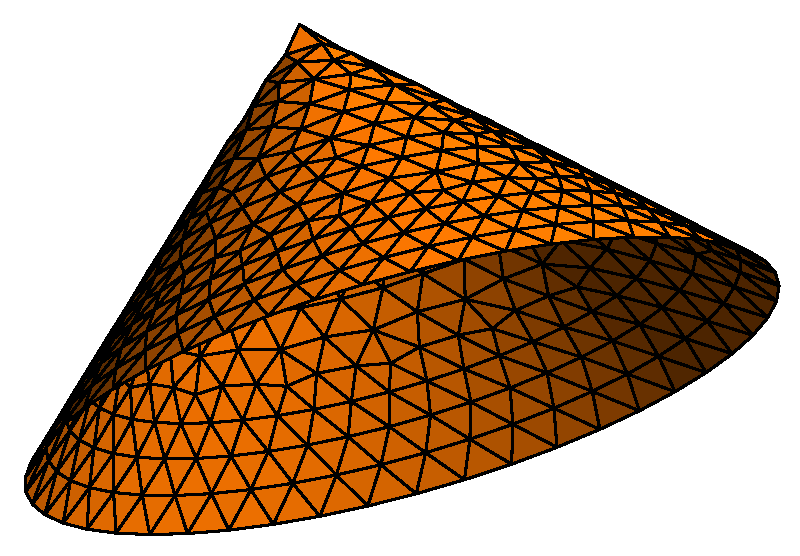
\includegraphics[width=90mm]{cone}
  \caption{A singularity (vertex)}
  \label{\numb section 3.\numb fig 9}
\end{figure}

\begin{Verbatim}[commandchars=\\\{\},formatcom=\small\tt,frame=single,
   label=code not working,rulecolor=\color{moldura},
   baselinestretch=0.94,framesep=2mm                                  ]
   \verm{Manifold} \azul{cone_manif} = RR3 .implicit ( x*x + y*x == z*z );

   cone_manif .implicit ( z == \laranja{1.} );
   \verm{Cell} \azul{A} ( \textcolor{tag}{tag}::vertex );  x (A) = \laranja{1.};  y (A) = \laranja{0.};  z (A) = \laranja{1.};
   \verm{Mesh} \azul{circle} ( \textcolor{tag}{tag}::frontal, \textcolor{tag}{tag}::start_at, A,
                 \textcolor{tag}{tag}::towards, \{ \laranja{0.}, \laranja{-1.}, \laranja{0.} \},
                 \textcolor{tag}{tag}::desired_length, \laranja{0.1}       );

   cone_manif .set_as_working_manifold();
   \verm{Cell} \azul{V} ( \textcolor{tag}{tag}::vertex );  x (V) = \laranja{0.};  y (V) = \laranja{0.};  z (V) = \laranja{0.};
   \verm{Mesh} \azul{cone} ( \textcolor{tag}{tag}::frontal, \textcolor{tag}{tag}::boundary, circle,
               \textcolor{tag}{tag}::start_at, A, \textcolor{tag}{tag}::towards, \{ \laranja{-1.}, \laranja{0.}, \laranja{-1.} \},
               \textcolor{tag}{tag}::singular, V, \textcolor{tag}{tag}::desired_length, \laranja{0.1}       );
\end{Verbatim}


                    %--------------------%
\section{~~\cinzasec{Singularities, again}}\label{\numb section 3.\numb parag 21}
                    %--------------------%

{\normalfont\bfseries The code described in this paragraph does not work yet.
It should be regarded as a mere declaration of intentions.}
\medskip

Besides vertices like the one described in paragraph \ref{\numb section 3.\numb parag 20},
another kind of singularity appears when we intersect two manifolds which have a tangency point.
This happens if we choose {\small\tt\azul{rc} = \laranja{0.5}} in paragraph
\ref{\numb section 3.\numb parag 18} or \ref{\numb section 3.\numb parag 19}.

We focus on the piece of cylinder from paragraph \ref{\numb section 3.\numb parag 19}
(which is to be subsequently {\small\tt join}ed with a sphere with two holes).

\begin{Verbatim}[commandchars=\\\{\},formatcom=\small\tt,frame=single,
   label=code not working,rulecolor=\color{moldura},
   baselinestretch=0.94,framesep=2mm                                  ]
   \verm{Manifold} \azul{cylinder} = RR3 .implicit ( y*y + (z-\laranja{0.5})*(z-\laranja{0.5}) == \laranja{0.25} );
   \verm{Manifold} \azul{infinity} = cylinder .implicit ( x*x + y*y + z*z == \laranja{1.} );

   \verm{Cell} \azul{V} ( \textcolor{tag}{tag}::vertex );  x (V) = \laranja{0.};  y (V) = \laranja{0.};  z (V) = \laranja{1.};
   \verm{Mesh} \azul{circle_1} ( \textcolor{tag}{tag}::frontal,
                   \textcolor{tag}{tag}:: start_at, V, \textcolor{tag}{tag}::towards, \{ \laranja{1.}, \laranja{1.}, \laranja{0.} \},
                   \textcolor{tag}{tag}::singular, V, \textcolor{tag}{tag}::desired_length, \laranja{0.1}      );
   \verm{Mesh} \azul{circle_2} ( \textcolor{tag}{tag}::frontal,
                   \textcolor{tag}{tag}:: start_at, V, \textcolor{tag}{tag}::towards, \{ \laranja{-1.}, \laranja{-1.}, \laranja{0.} \},
                   \textcolor{tag}{tag}::singular, V, \textcolor{tag}{tag}::desired_length, \laranja{0.1}        );

   cylinder .set_as_working_manifold();
   \verm{Cell} \azul{W} = circle_1 .cell_in_front_of (V) .tip();
   \verm{Mesh} \azul{piece_of_cyl} ( \textcolor{tag}{tag}::frontal, \textcolor{tag}{tag}::boundary, circle_1, circle_2,
                       \textcolor{tag}{tag}::start_at, W, \textcolor{tag}{tag}::towards, \{ \laranja{-1.}, \laranja{1.}, \laranja{0.} \},
                       \textcolor{tag}{tag}::singular, V, \textcolor{tag}{tag}::desired_length, \laranja{0.1}      );
\end{Verbatim}

\begin{figure}[ht] \centering
 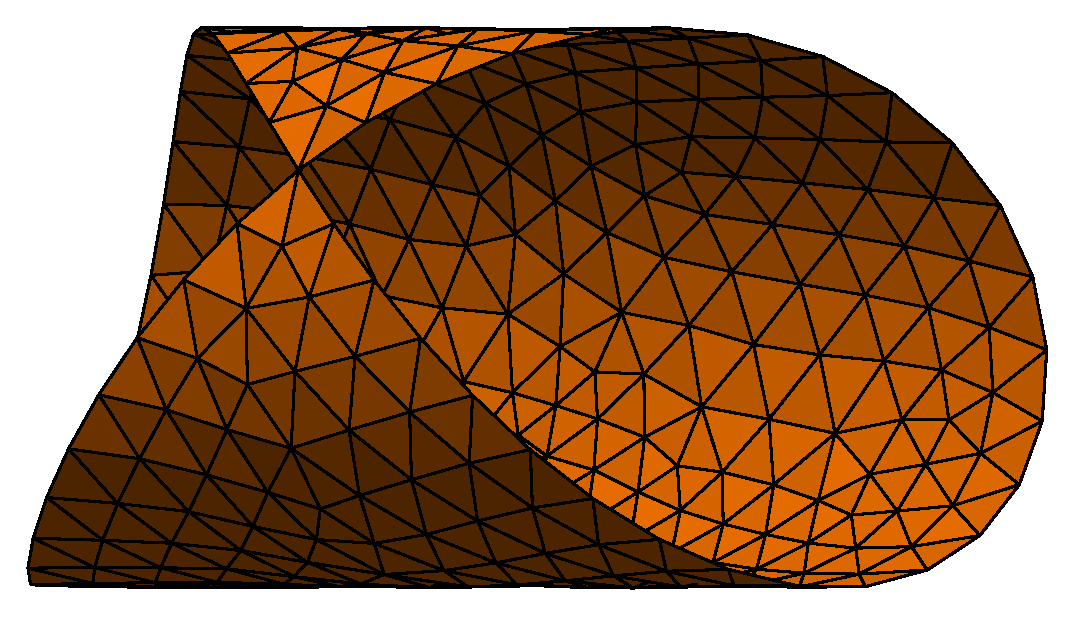
\includegraphics[width=85mm]{cyl}
  \caption{A singularity (napkin)}
  \label{\numb section 3.\numb fig 10}
\end{figure}

{\ManiFEM} accepts as {\small\tt\verm{Manifold}} a self-intersecting set like {\small\tt infinity}.
In {\maniFEM}, an implicit manifold is simply a level set of one or two symbolic expressions
involving the coordinates of the surrounding, Euclidean manifold.
However, in the neighbourhood of a singularity, the equation(s) are degenerate and certain
parts of {\maniFEM} do not work as expected.
In particular, the projection algorithm onto the manifold may fail to converge.
By specifying (in the {\small\tt\verm{Mesh}} constructor) {\small\tt V} as singular point,
we tell {\maniFEM} that it must take special care in that neighbourhood.

Unlike in paragraph \ref{\numb section 3.\numb parag 19}, here we cannot {\small\tt join} the
two meshes {\small\tt circle\_\,1} and {\small\tt circle\_\,2}.
{\ManiFEM} is unable to join two closed polygonal lines having a vertex in common;
in other words, it does not handle self-intersecting {\small\tt\verm{Mesh}}es.
This is why we provide the two pieces of boundary separately.


          %-------------------%
\section{~~Non-uniform meshing}\label{\numb section 3.\numb parag 22}
          %-------------------%

The desired length may be a non-constant function.

\begin{figure}[ht] \centering
 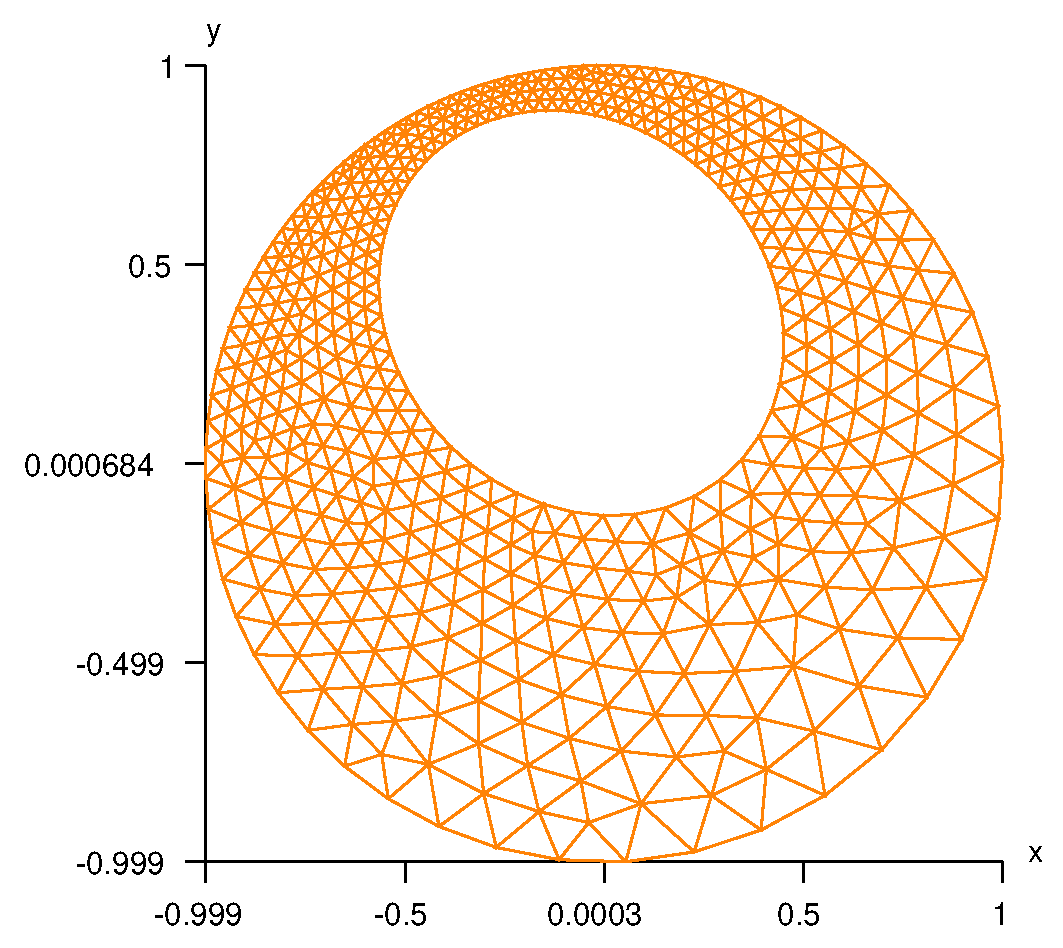
\includegraphics[width=90mm]{disk-non-unif}
  \caption{Non-uniform mesh}
  \label{\numb section 3.\numb fig 11}
\end{figure}

\begin{Verbatim}[commandchars=\\\{\},formatcom=\small\tt,frame=single,
   label=parag-\ref{\numb section 3.\numb parag 22}.cpp,rulecolor=\color{moldura},
   baselinestretch=0.94,framesep=2mm                                            ]
   \verm{Function} \azul{d} = \laranja{0.03} + \laranja{0.04} * ( (x+\laranja{0.3})*(x+\laranja{0.3}) + (y-\laranja{0.9})*(y-\laranja{0.9}) );

   \verm{Manifold} \azul{circle} = RR2 .implicit ( x*x + y*y == \laranja{1.} );
   \verm{Mesh} \azul{outer} ( \textcolor{tag}{tag}::frontal, \textcolor{tag}{tag}::desired_length, d );

   \verm{Manifold} \azul{ellipse} = RR2 .implicit ( x*x + (y-\laranja{0.37})*(y-\laranja{0.37}) + \laranja{0.3}*x*y == \laranja{0.25} );
   \verm{Mesh} \azul{inner} ( \textcolor{tag}{tag}::frontal, \textcolor{tag}{tag}::desired_length, d );
   \verm{Mesh} \azul{bdry} ( \textcolor{tag}{tag}::join, outer, inner .reverse() );

   RR2 .set_as_working_manifold();
   \verm{Mesh} \azul{disk} ( \textcolor{tag}{tag}::frontal, \textcolor{tag}{tag}::boundary, bdry, \textcolor{tag}{tag}::desired_length, d );
\end{Verbatim}

Compare with the mesh in paragraph \ref{\numb section 3.\numb parag 3}.

It is the user's responsibility to provide a length {\small\tt d} which takes positive values
at all points of the future mesh.
Also, {\small\tt d} should be a reasonably smooth function; sharp variations should be avoided.


          %-------------------------%
% \section{~~Two intersecting tori}\label{\numb section 3.\numb parag 22}
          %-------------------------%

% Going back to the two tori in paragraph \ref{\numb section 3.\numb parag 7},
% we now build the edges first and obtain a sharp, precise cut
% (forget about {\small\tt\verm{smooth\_\,min}}).

% \begin{figure}[ht] \centering
%  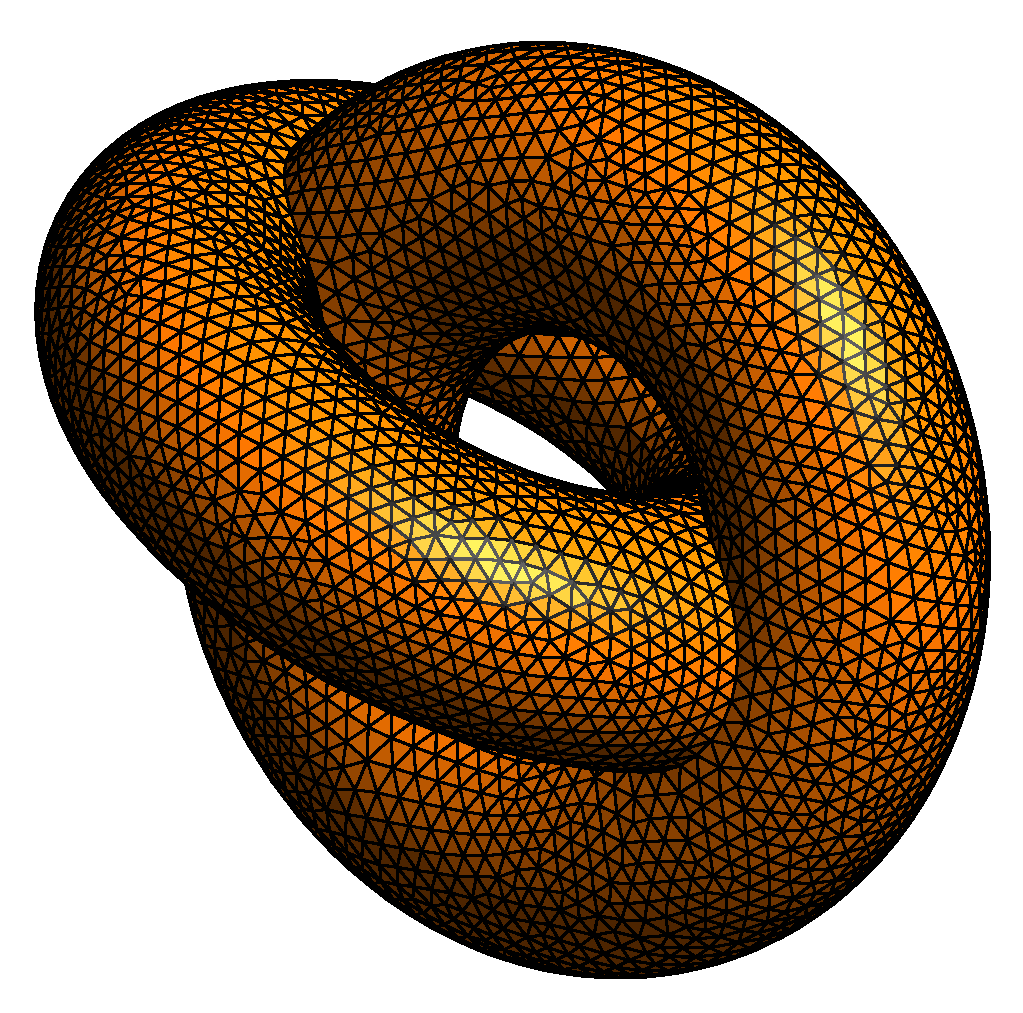
\includegraphics[width=79mm]{two-tori-sharp}
%   \caption{Sharp edges}
%   \label{\numb section 3.\numb fig 8}
% \end{figure}


                    %---------------------------%
\section{~~\cinzasec{Changing the Riemann metric}}\label{\numb section 3.\numb parag 23}
                    %---------------------------%
 
{\normalfont\bfseries The code described in this paragraph does not work yet.
It should be regarded as a mere declaration of intentions.}
\medskip

We can attach a non-uniform metric to our manifold; as a consequence, for a constant
{\small\tt desired\_\,length}, the apparent segment length will vary from zone to zone.
For instance, in the code below we set a metric which increases the measured length
of the segments close to the narrow part of the domain.
As a consequence, the meshing algorithm, while trying to build a mesh of constant
{\small\tt desired\_\,length}, will choose shorter segments in the proximity of the narrow zone
(because the length measured by the Riemann metric will be larger than the length
we see in the drawing), thus producing the same result as in paragraph
\ref{\numb section 3.\numb parag 22}.

\begin{Verbatim}[commandchars=\\\{\},formatcom=\small\tt,frame=single,
   label=code not working,rulecolor=\color{moldura},
   baselinestretch=0.94,framesep=2mm                                   ]
   \verm{Manifold} \azul{RR2} ( \textcolor{tag}{tag}::Euclid, \textcolor{tag}{tag}::of_dim, \laranja{2} );
   \verm{Function} \azul{xy} = RR2 .build_coordinate_system ( \textcolor{tag}{tag}::Lagrange, \textcolor{tag}{tag}::of_degree, \laranja{1} );
   \verm{Function} \azul{x} = xy [\laranja{0}], \azul{y} = xy [\laranja{1}];

   \verm{Function} \azul{d} = \laranja{0.3} + \laranja{0.5} * ( (x+\laranja{0.3})*(x+\laranja{0.3}) + (y-\laranja{0.9})*(y-\laranja{0.9}) );
   RR2 .set_metric ( \laranja{1.} / d );
   
   \verm{Manifold} \azul{circle} = RR2 .implicit ( x*x + y*y == \laranja{1.} );
   \verm{Mesh} \azul{outer} ( \textcolor{tag}{tag}::frontal, \textcolor{tag}{tag}::desired_length, \laranja{0.1} );
   \verm{Manifold} \azul{ellipse} = RR2 .implicit ( x*x + (y-\laranja{0.37})*(y-\laranja{0.37}) + \laranja{0.3}*x*y == \laranja{0.25} );
   \verm{Mesh} \azul{inner} ( \textcolor{tag}{tag}::frontal, \textcolor{tag}{tag}::desired_length, \laranja{0.1} );

   \verm{Mesh} \azul{bdry} ( \textcolor{tag}{tag}::join, outer, inner .reverse() );

   RR2 .set_as_working_manifold();
   \verm{Mesh} \azul{disk} ( \textcolor{tag}{tag}::frontal, \textcolor{tag}{tag}::boundary, bdry, \textcolor{tag}{tag}::desired_length, \laranja{0.1} );
\end{Verbatim}

These two approaches (the one described in paragraph \ref{\numb section 3.\numb parag 22} and
the one described here) can be used interchangeably.
It is possible to use both in the same code, but the code will become rather obscure.


                    %------------------%
\section{~~\cinzasec{Anisotropic metric}}\label{\numb section 3.\numb parag 24}
                    %------------------%

{\normalfont\bfseries The code described in this paragraph does not work yet.
It should be regarded as a mere declaration of intentions.}
\medskip

The technique described in paragraph \ref{\numb section 3.\numb parag 23} can be generalized to
an anisotropic Riemann metric.
We define the metric by means of a square matrix $M$.
$M$ must be symmetric positive definite.
The arguments of {\small\tt set\_\,metric} are $ m_{11} $, $ m_{12} $ and $ m_{22} $
for two dimensions,
$ m_{11} $, $ m_{12} $, $ m_{13} $, $ m_{22} $, $ m_{23} $ and $ m_{33} $ for three dimensions.

\begin{figure}[ht] \centering
 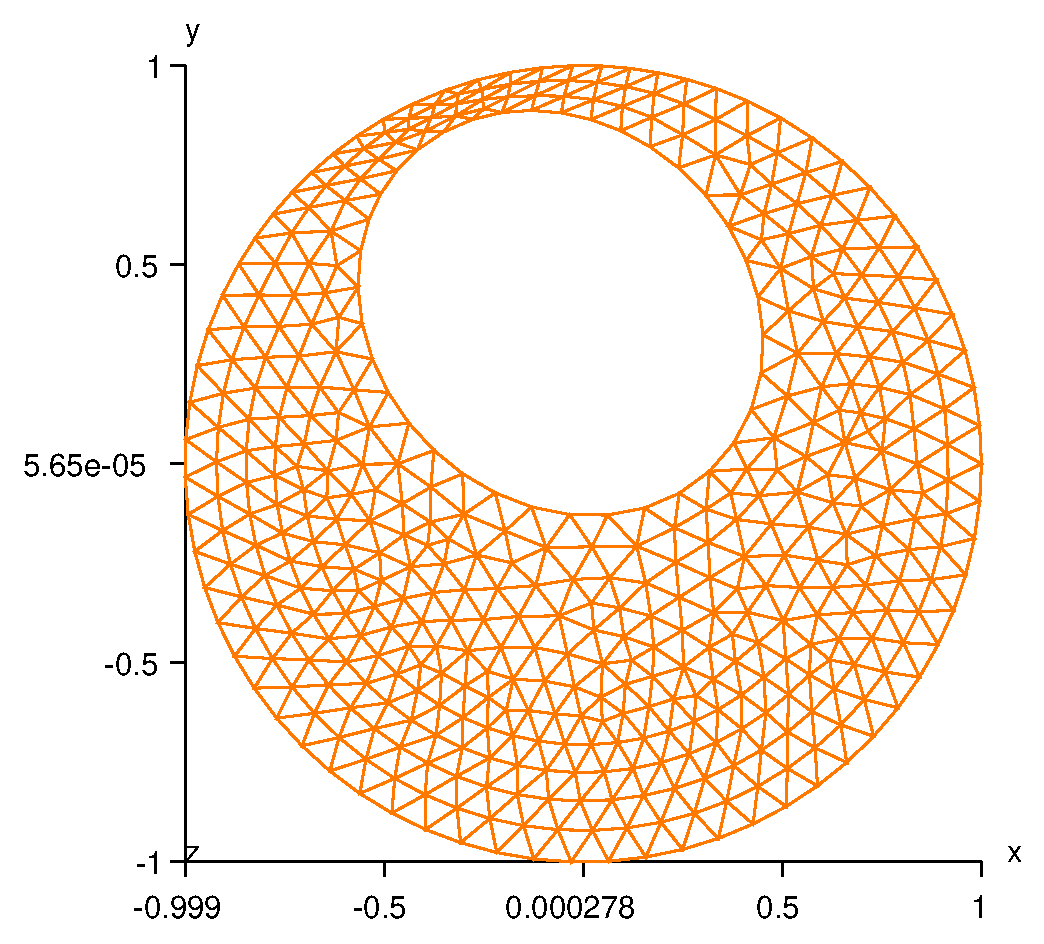
\includegraphics[width=90mm]{disk-anisotrop}
  \caption{Anisotropic mesh}
  \label{\numb section 3.\numb fig 12}
\end{figure}

\begin{Verbatim}[commandchars=\\\{\},formatcom=\small\tt,frame=single,
   label=code not working,rulecolor=\color{moldura},
   baselinestretch=0.94,framesep=2mm                                  ]
   \verm{Manifold} \azul{RR2} ( \textcolor{tag}{tag}::Euclid, \textcolor{tag}{tag}::of_dim, \laranja{2} );
   \verm{Function} \azul{xy} = RR2 .build_coordinate_system ( \textcolor{tag}{tag}::Lagrange, \textcolor{tag}{tag}::of_degree, \laranja{1} );
   \verm{Function} \azul{x} = xy [\laranja{0}], \azul{y} = xy [\laranja{1}];

   \verm{Function} \azul{d} = \laranja{0.3} + (x+\laranja{0.3})*(x+\laranja{0.3}) + (y-\laranja{0.9})*(y-\laranja{0.9});
   RR2 .set_metric ( \laranja{1.} + \laranja{1.}/d, \laranja{-3.}/d, \laranja{1.} + \laranja{9.}/d );
   \cinza{// or, equivalently :}
   \cinza{// RR2 .set_metric ( tag::principal_part, 1.,}
   \cinza{//                   tag::deviatoric_part, 1./d, -3./d, 9./d );}
   \verm{Manifold} \azul{circle} = RR2 .implicit ( x*x + y*y == \laranja{1.} );
   \verm{Mesh} \azul{outer} ( \textcolor{tag}{tag}::frontal, \textcolor{tag}{tag}::desired_length, \laranja{0.1} );
   \verm{Manifold} \azul{ellipse} = RR2 .implicit ( x*x + (y-\laranja{0.37})*(y-\laranja{0.37}) + \laranja{0.3}*x*y == \laranja{0.25} );
   \verm{Mesh} \azul{inner} ( \textcolor{tag}{tag}::frontal, \textcolor{tag}{tag}::desired_length, \laranja{0.1} );
   \verm{Mesh} \azul{bdry} ( \textcolor{tag}{tag}::join, outer, inner .reverse() );

   RR2 .set_as_working_manifold();
   \verm{Mesh} \azul{disk} ( \textcolor{tag}{tag}::frontal, \textcolor{tag}{tag}::boundary, bdry, \textcolor{tag}{tag}::desired_length, \laranja{0.1} );
\end{Verbatim}

Compare with the mesh in paragraph \ref{\numb section 3.\numb parag 3}.

This result cannot be achieved using the approach of paragraph
\ref{\numb section 3.\numb parag 22} (by setting a non-constant desired length).


          %-----------%
\section{~~Future work}\label{\numb section 3.\numb parag 25}
          %-----------%

It would be nice to define domains using inequalities between {\small\tt\verm{Function}}s.



                  %------------------------------------%
\chapter {~~\cinza{Meshing three-dimensional domains}}\label{\numb section 4}
                  %------------------------------------%

Work in progress.



          %----------------------------------------------%
\chapter{~~Fields, functions and variational formulations}\label{\numb section 5}
          %----------------------------------------------%


          %--------------------%
\section{~~Fields and functions}\label{\numb section 5.\numb parag 1}
          %--------------------%

As the reader may have already noticed, all examples in {\maniFEM} begin by declaring a
Euclidian {\small\tt \verm{Manifold}} and then go on by building a coordinate system :

\begin{Verbatim}[commandchars=\\\{\},formatcom=\small\tt,
   baselinestretch=0.94,framesep=2mm                     ]
   \verm{Manifold} RR2 ( \textcolor{tag}{tag}::Euclid, \textcolor{tag}{tag}::of_dim, \laranja{2} );
   \verm{Function} \azul{xy} = RR2 .build_coordinate_system ( \textcolor{tag}{tag}::Lagrange, \textcolor{tag}{tag}::of_degree, \laranja{1} );
   \verm{Function} \azul{x} = xy [\laranja{0}], \azul{y} = xy [\laranja{1}];
\end{Verbatim}

See paragraph \numb section 11.\numb parag 3 for more details about tags.

In the above, {\small\tt \verm{xy}} is a {\small\tt \verm{Function}}, a vector field actually,
with two components, {\small\tt x} and {\small\tt y}.
The declaration of {\small\tt xy} starts a complex process; under the curtains
{\maniFEM} declares a {\small\tt \verm{Field}} object associated to {\small\tt xy}.
The {\small\tt \verm{Field}} object changes the behaviour of {\maniFEM} in what regards
initialization of {\small\tt \verm{Cell}}s.
Since {\small\tt xy} is of type Lagrange of degree 1, each newly built vertex
{\small\tt \verm{Cell}} will have memory space reserved for two {\small\tt double}
precision numbers.
If {\small\tt A} is a vertex {\small\tt \verm{Cell}}, an assignment like {\small\tt x(A) = \laranja{1.5}}
sets the value of the {\small\tt x} component of the {\small\tt \verm{Field}} associated to
{\small\tt xy} at {\small\tt A}.

If we declare {\small\tt xy} to be of type Lagrange of degree 2, not only future vertices will
have space reserved for two {\small\tt double}s, but also future segments.
So, we may assign the value of {\small\tt y} at the middle of segment {\small\tt AB} by using
the syntax {\small\tt y(AB) = \laranja{0.75}}.

{\small\tt \verm{Function}} objects allow for arithmetic expressions like in

\begin{Verbatim}[commandchars=\\\{\},formatcom=\small\tt,
   baselinestretch=0.94,framesep=2mm                     ]
   \verm{Function} \azul{norm} = \verm{power} ( x*x + y*y, \laranja{0.5} );
\end{Verbatim}

The {\small\tt deriv} method performs symbolic differentiation :

\begin{Verbatim}[commandchars=\\\{\},formatcom=\small\tt,
   baselinestretch=0.94,framesep=2mm                     ]
   \verm{Function} \azul{norm_x} = norm .deriv ( x );
   \verm{Function} \azul{norm_y} = norm .deriv ( y );
\end{Verbatim}

Functions can also be integrated, see section \numb section 6.




          %-------------------------------%
\chapter{~~Finite elements and integrators}\label{\numb section 6}
          %-------------------------------%


Finite elments are still incipient in \maniFEM.
Paragraph \ref{\numb section 6.\numb parag 1} discusses the concept of finite element
and paragraphs \ref{\numb section 6.\numb parag 2} -- \ref{\numb section 6.\numb parag 4}
give examples of rudimentary use.
There is a lot of ongoing work on this subject.


          %---------------%
\section{~~Finite elements}\label{\numb section 6.\numb parag 1}
          %---------------%

The notion of a finite element is quite complex.
The purpose of a {\small\tt \verm{FiniteElement}} is to build a list of functions, say, $ \psi $,
defined on our mesh.
The linear span of these functions will be a discretized Hilbert space.
It is the {\small\tt \verm{FiniteElement}}'s job to replace, in the variational formulation,
the unknown function by one $ \psi $, the test function by another $ \psi $ and,
by evaluating the integrals, obtain the coefficients of a system of linear equations.
Some external solver will then solve the system, and it is the job of the finite element
to transform back the vector produced by the solver into a function defined on our mesh.

Computing each integral is a somewhat separate process; it's the job of an
{\small\tt \verm{Integrator}}
which could be a Gauss quadrature or some other procedure like symbolic integration.
When a Gauss quadrature is used, the separation between a {\small\tt \verm{FiniteElement}}'s job
and the {\small\tt \verm{Itegrator}}'s job is not very sharp because often the Gauss quadrature is
perfomed not on the physical cell but rather on a master element which is built and
handled by the {\small\tt \verm{FiniteElement}}.
The authors of {\maniFEM} have tried to separate these two concepts
as much as possible, especially because some users may want to use a {\small\tt \verm{FiniteElement}}
with no master element, or an {\small\tt \verm{Integrator}} acting directly on the physical cell.

Thus, there is a base class {\small\tt \verm{FiniteElement}} and a derived class
{\small\tt \verm{FiniteElement}::withMaster} which keeps, as an extra attribute, the map transforming
the master element to the current physical cell.
This map depends of course on the geometry of the cell and thus it must be computed from
scratch each time we begin integrating on a new cell.
We say that the {\small\tt \verm{FiniteElement}} is docked on a new {\small\tt \verm{Cell}};
the method {\small\tt dock\_\,on} performs this operation.
This method is element-specific, each type of finite element having its own class.

For instance, the class {\small\tt \verm{FiniteElement}::Lagrange\_\,Q1} is a class derived from
{\small\tt \verm{FiniteElement}:: ::withMaster}.
It will only {\small\tt dock\_\,on} quadrilaterals (two-dimensional {\small\tt \verm{Cell}}s
with four sides).
% Recall that in {\maniFEM} the vertices do not have necessarily any number attached.
% When we create a {\small\tt \verm{FiniteElement}::Lagrange\_\,Q1} object, it will enumerate vertices
% of the mesh if a mesh exists already, and it will prepare the ground for vertices created
% in the future to be enumerated, too.
% This enumeration is useful to identify a vector of real numbers with the values
% (at each vertex) of a function defined on the mesh.
When docking on a cell, the {\small\tt \verm{FiniteElement}::Lagrange\_\,Q1} object will build four
``shape functions'' and a transformation map (a diffeomorphism between a master element
occuppying the square $ [-1, 1]^2 $ and the current cell).
It will also build the jacobian of this transformation map.
The four shape functions can be accessed through the method {\small\tt basis\_\,function},
as shown in paragraph \ref{\numb section 6.\numb parag 2}.

It should be stressed that the approach presented in this section is rather low-level.
We are working hard to make {\maniFEM} understand statements describing variational
formulations given as {\tt C++} objects.
When this part of the code is done, the programming style will become much more elegant
and compact.

Note also that these examples make use of the {\small\tt Eigen} library.


          %------------------------------------------------%
\section{~~Laplace operator, Dirichlet boundary conditions}\label{\numb section 6.\numb parag 2}
          %------------------------------------------------%
\vskip 1mm

Let's look at an example about the Laplace operator with non-homogeneous Dirichlet
boundary conditions.
\vskip 1mm

\begin{Verbatim}[commandchars=\\\{\},formatcom=\small\tt,frame=single,
   label=parag-\ref{\numb section 6.\numb parag 2}.cpp,rulecolor=\color{coment},
   baselinestretch=0.94,framesep=2mm                                            ]
   \verm{Manifold} \azul{RR2} ( \textcolor{tag}{tag}::Euclid, \textcolor{tag}{tag}::of_dim, 2 );
   \verm{Function} \azul{xy} = RR2 .build_coordinate_system ( \textcolor{tag}{tag}::Lagrange, \textcolor{tag}{tag}::of_degree, 1 );
   \verm{Function} \azul{x} = xy [0], \azul{y} = xy [1];

   \cinza{// declare the type of finite element}
   \verm{FiniteElement} \azul{fe}
      ( \textcolor{tag}{tag}::with_master, \textcolor{tag}{tag}::quadrangle, \textcolor{tag}{tag}::Lagrange, \textcolor{tag}{tag}::of_degree, 1 );
   \verm{Integrator} \azul{integ} = fe .set_integrator ( \textcolor{tag}{tag}::Gauss, \textcolor{tag}{tag}::quad_4 );

   \cinza{// build a 10x12 mesh on a square domain}
   \verm{Cell} \azul{A} ( \textcolor{tag}{tag}::vertex );  x (A) = 0.;   y (A) = 0.;
   \verm{Cell} \azul{B} ( \textcolor{tag}{tag}::vertex );  x (B) = 1.;   y (B) = 0.;
   \verm{Cell} \azul{C} ( \textcolor{tag}{tag}::vertex );  x (C) = 1.;   y (C) = 1.;
   \verm{Cell} \azul{D} ( \textcolor{tag}{tag}::vertex );  x (D) = 0.;   y (D) = 1.;
   \verm{Mesh} \azul{AB} ( \textcolor{tag}{tag}::segment, A .reverse(), B, \textcolor{tag}{tag}::divided_in, 10 );
   \verm{Mesh} \azul{BC} ( \textcolor{tag}{tag}::segment, B .reverse(), C, \textcolor{tag}{tag}::divided_in, 12 );
   \verm{Mesh} \azul{CD} ( \textcolor{tag}{tag}::segment, C .reverse(), D, \textcolor{tag}{tag}::divided_in, 10 );
   \verm{Mesh} \azul{DA} ( \textcolor{tag}{tag}::segment, D .reverse(), A, \textcolor{tag}{tag}::divided_in, 12 );
   \verm{Mesh} \azul{ABCD} ( \textcolor{tag}{tag}::rectangle, AB, BC, CD, DA );
\end{Verbatim}
\vskip 1mm

A finite element can handle by itself the numbering of vertices, as shown in paragraph
\ref{\numb section 6.\numb parag 4}.
For now, we prefer the conceptually simpler approach of building by hand a {\small\tt map}
for numbering vertices.
\vskip 1mm

\begin{Verbatim}[commandchars=\\\{\},formatcom=\small\tt,frame=single,
   label=parag-\ref{\numb section 6.\numb parag 2}.cpp,rulecolor=\color{coment},
   baselinestretch=0.94,framesep=2mm                                            ]
   std::map < Cell, size_t > \azul{numbering};
   \verm{CellIterator} \azul{it} = ABCD .iterator ( \textcolor{tag}{tag}::over_vertices );
   size_t \azul{counter} = 0;
   for ( it .reset() ; it .in_range(); it++ )
   \{  \verm{Cell} \azul{V} = *it;  numbering [V] = counter;  ++counter;  \}
\end{Verbatim}
\vskip 1mm

The matrix of the linear system and the vector holding the free coefficients
are declared as objects of the {\small\tt Eigen} library.

\begin{Verbatim}[commandchars=\\\{\},formatcom=\small\tt,frame=single,
   label=parag-\ref{\numb section 6.\numb parag 2}.cpp,rulecolor=\color{coment},
   baselinestretch=0.94,framesep=2mm                                            ]
   size_t \azul{size_matrix} = ABCD .number_of ( \textcolor{tag}{tag}::vertices );
   assert ( size_matrix == numbering .size() );
   Eigen::SparseMatrix < double > \azul{matrix_A} ( size_matrix, size_matrix );
   Eigen::VectorXd \azul{vector_b} ( size_matrix );  vector_b .setZero();
\end{Verbatim}
\vskip 1mm

We now run over all rectangular cells of {\small\tt ABCD}, dock the finite element
on the current cell,
compute integrals of the form $ \displaystyle \int\!\!\!\int {\partial \psi_i \over
\partial x_\alpha} {\partial \psi_j \over \partial x_\beta} dx $ and add the obtained
values to the global matrix:
\vskip 1mm

\begin{Verbatim}[commandchars=\\\{\},formatcom=\small\tt,frame=single,
   label=parag-\ref{\numb section 6.\numb parag 2}.cpp,rulecolor=\color{coment},
   baselinestretch=0.94,framesep=2mm                                            ]
   // run over all square cells composing ABCD
   \verm{CellIterator} \azul{it} = ABCD .iterator ( \textcolor{tag}{tag}::over_cells_of_dim, 2 );
   for ( it .reset(); it .in_range(); it++ )
   \{  \verm{Cell} \azul{small_square} = *it;
      fe .dock_on ( small_square );
      // run twice over the four vertices of 'small_square'
      \verm{CellIterator} \azul{it1} = small_square .boundary() .iterator ( \textcolor{tag}{tag}::over_vertices );
      \verm{CellIterator} \azul{it2} = small_square .boundary() .iterator ( \textcolor{tag}{tag}::over_vertices );
      for ( it1 .reset(); it1 .in_range(); it1++ )
      for ( it2 .reset(); it2 .in_range(); it2++ )
      \{  \verm{Cell} \azul{V} = *it1, \azul{W} = *it2;
         \cinza{// V may be the same as W, no problem about that}
         \verm{Function} \azul{psiV} = fe.basis_function(V),
                  \azul{psiW} = fe .basis_function (W),
                  \azul{d_psiV_dx} = psiV .deriv (x),
                  \azul{d_psiV_dy} = psiV .deriv (y),
                  \azul{d_psiW_dx} = psiW .deriv (x),
                  \azul{d_psiW_dy} = psiW .deriv (y);
                  
         \cinza{// 'fe' is already docked on 'small_square'}
         \cinza{// so this will be the domain of integration}
         matrix_A .coeffRef ( numbering[V], numbering[W] ) +=
            fe .integrate ( d_psiV_dx * d_psiW_dx + d_psiV_dy * d_psiW_dy );    \}  \}
\end{Verbatim}

In the above, {\small\tt coeffRef} is the method used by {\small\tt Eigen} to access elements of
a sparse matrix.

We impose Dirichlet boundary conditions $ u(x,y) = xy $ (this way, we know beforehand
the exact solution will be $ u(x,y) = xy $).
We use a function {\small\tt impose\_\,value\_\,of\_\,unknown} which changes the {\small\tt matrix\_\,A}
and the {\small\tt vector\_\,b} in order to impose the Dirichlet condition {\small\tt u(i) = 
some\_\,value}.
See the source code in file {\small\tt main-\ref{\numb section 6.\numb parag 2}.cpp}
in the distribution tree for the definition of the {\small\tt impose\_\,value\_\,of\_\,unknown}
function.

\begin{Verbatim}[commandchars=\\\{\},formatcom=\small\tt,frame=single,
   label=parag-\ref{\numb section 6.\numb parag 2}.cpp,rulecolor=\color{coment},
   baselinestretch=0.94,framesep=2mm                                            ]
   \verm{CellIterator} \azul{it} = BC .iterator ( \textcolor{tag}{tag}::over_vertices );
   for ( it .reset(); it .in_range(); it++ )
   \{   \verm{Cell} \azul{P} = *it;
       size_t \azul{i} = numbering [P];
       impose_value_of_unknown ( matrix_A, vector_b, i, y(P) );  \}
\end{Verbatim}

We then use {\small\tt Eigen} to solve the system of linear equations :

\begin{Verbatim}[commandchars=\\\{\},formatcom=\small\tt,frame=single,
   label=parag-\ref{\numb section 6.\numb parag 2}.cpp,rulecolor=\color{coment},
   baselinestretch=0.94,framesep=2mm                                            ]
   Eigen::ConjugateGradient < Eigen::SparseMatrix <double>,
                              Eigen::Lower | Eigen::Upper  > \azul{cg};
   cg .compute ( matrix_A );
   Eigen::VectorXd \azul{u} = cg .solve ( vector_b );
\end{Verbatim}

And obtain the expected solution, shown in figure \ref{\numb section 6.\numb fig 1}.

\begin{figure} \centering
  \psfrag{A}{\small\tt\textcolor{textindraw}{A}}
  \psfrag{B}{\small\tt\textcolor{textindraw}{B}}
  \psfrag{C}{\small\tt\textcolor{textindraw}{C}}
  \psfrag{D}{\small\tt\textcolor{textindraw}{D}}
  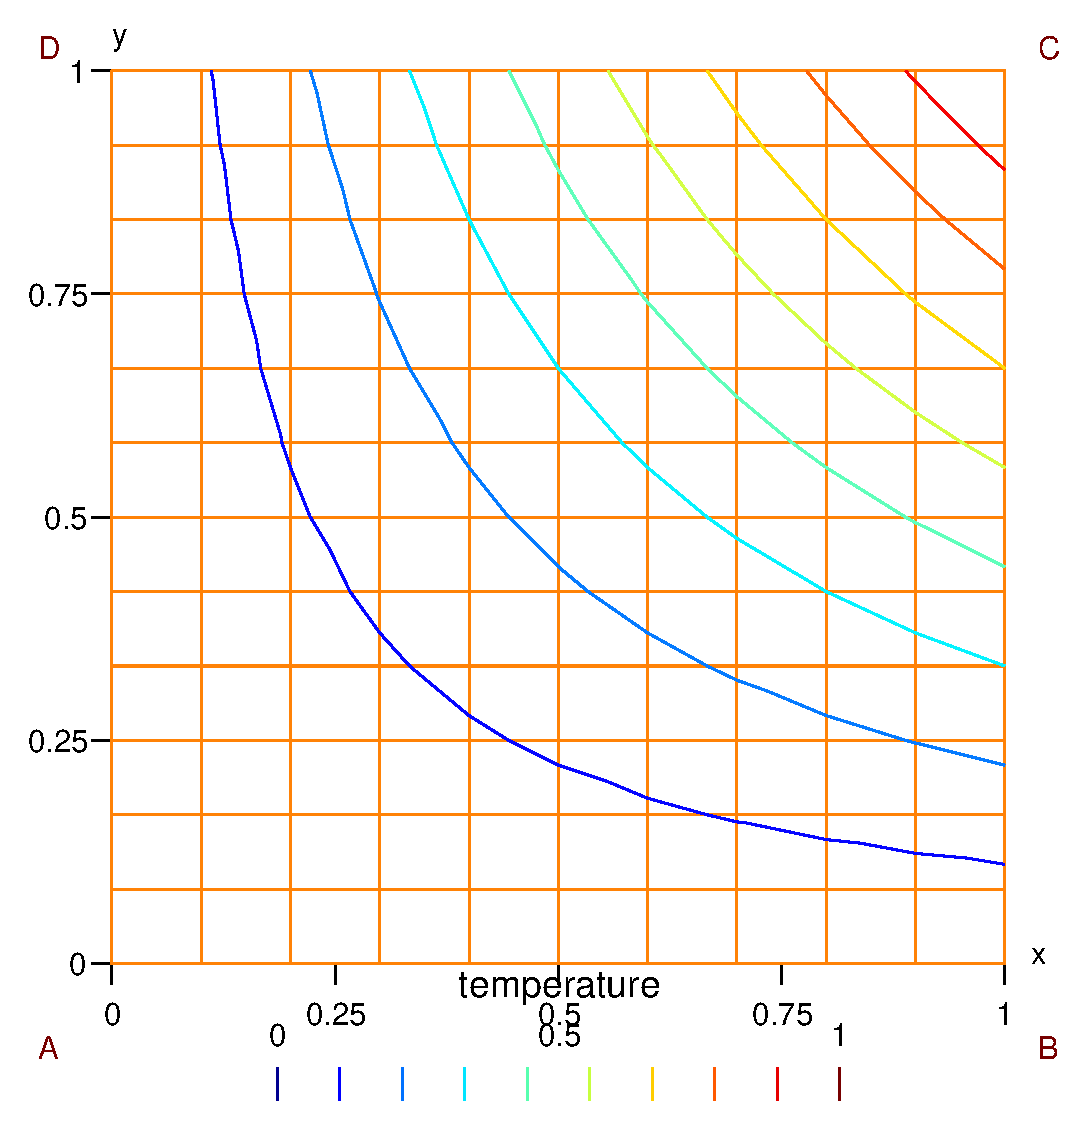
\includegraphics[width=60mm]{square-Dirichlet}
  \caption{Level lines of $u$}
  \label{\numb section 6.\numb fig 1}
\end{figure}

We stress again that this example shows a rather rudimentary way of using finite elements in
\maniFEM.
We are working hard to reach a more elegant, compact and high-level style.
The user should have the possibility to declare the partial differential equation
through a compact declaration of the corresponding variational formulation.

Another limitation of {\maniFEM} is that, at present, finite element computations
are rather slow.
This is so because each docking operation implies a lot of symbolic calculations;
the same happens when we differentiate and then integrate functions.
There are three ways of circumventing this limitation.
The first one is : if your mesh is made of identical finite elements
(like the example in the present paragraph), you can compute the elementary matrix
just once and then assembly the global matrix from it.
It will surely be much faster.
A second way to speed up the code is to add the option {\small\tt -dNDEBUG} to the compilation
command in your {\small\tt Makefile} (see also paragraph \ref{\numb section 11.\numb parag 15}).

The third (and soundest) solution is a deep optimization of the {\maniFEM} library.
A new type of finite elements (or, rather, integrators) is object of on-going work.
These integrators perform a few symbolic calculations just once,
typically right after they are declared.
Only raw arithmetic operations are performed when the user actually requests the values
of integrals in order to assembly the matrix.


          %---------------------------%
\section{~~Neumann boundary conditions}\label{\numb section 6.\numb parag 3}
          %---------------------------%

Implementing zero Neumann boundary conditions does not imply any programming effort
(we don't have to do anything).
However, for imposing non-zero Neumann boundary conditions we need to compute one-dimensional
integrals.
We do this by declaring a 1D finite element which we then dock on each segment of the
part of the boundary where we need to integrate.

\begin{Verbatim}[commandchars=\\\{\},formatcom=\small\tt,frame=single,
   label=parag-\ref{\numb section 6.\numb parag 3}.cpp,rulecolor=\color{coment},
   baselinestretch=0.94,framesep=2mm                                            ]
   \verm{FiniteElement} \azul{fe_bdry} ( \textcolor{tag}{tag}::with_master, \textcolor{tag}{tag}::segment,
                           \textcolor{tag}{tag}::Lagrange, \textcolor{tag}{tag}::of_degree, 1 );
   \verm{Integrator} \azul{integ_bdry} = fe_bdry .set_integrator ( \textcolor{tag}{tag}::Gauss, \textcolor{tag}{tag}::seg_3 );

   \cinza{// ... assemble the matrix ...}

   \verm{Function} \azul{heat_source} = x+y;
   \cinza{// impose Neumann boundary conditions du/dn = heat_source :}
   \verm{CellIterator} \azul{it} = DA .iterator ( \textcolor{tag}{tag}::over_segments );
   for ( it .reset(); it .in_range(); it++ )
   \{  \verm{Cell} \azul{seg} = *it;
      fe_bdry .dock_on ( seg );
      \verm{Cell} \azul{V} = seg .base() .reverse();
      assert ( V .is_positive() );
      size_t \azul{i} = numbering [V];
      \verm{Function} \azul{psiV} = fe_bdry .basis_function(V);
      vector_b[i] += fe_bdry.integrate ( heat_source * psiV );
      \verm{Cell} \azul{W} = seg.tip();
      assert ( W .is_positive() );
      size_t \azul{j} = numbering [W];
      \verm{Function} \azul{psiW} = fe_bdry .basis_function(W);
      vector_b [j] += fe_bdry .integrate ( heat_source * psiW );  \}
\end{Verbatim}

One may object that there is no need for a 1D finite element, a 1D integrator should be enough.
We agree; the user should have the possibility to attach a 1D integrator to a 2D finite element.
This is object of on-going work.


          %------------------------------%
\section{~~Automatic numberig of vertices}\label{\numb section 6.\numb parag 4}
          %------------------------------%

In previous examples we have built a {\small\tt map} for handling numbering of vertices.
In this paragraph we show how to use instead the automatic numbering associated to the
finite element itself.
After declaring a finite element of type Lagrange with
{\small\tt\textcolor{tag}{tag}::enumerate\_\,cells},
the process of creating new cells (vertices, in this specfic case) will be different.
A new function will be added to the list of functions
{\small\tt\verm{Cell}::init\_\,pos\_\,cell[0]},
invoked by {\small\tt\verm{Cell}::Core} constructors
(see paragraph \ref{\numb section 11.\numb parag 10}).
Space will be reserved for a {\small\tt size\_\,t} value for each vertex, and
this value can be used for numbering vertices.

\begin{Verbatim}[commandchars=\\\{\},formatcom=\small\tt,frame=single,
   label=parag-\ref{\numb section 6.\numb parag 4}.cpp,rulecolor=\color{coment},
   baselinestretch=0.94,framesep=2mm                                            ]
   \verm{FiniteElement} \azul{fe} ( \textcolor{tag}{tag}::with_master, \textcolor{tag}{tag}::quadrangle,
                      \textcolor{tag}{tag}::Lagrange, \textcolor{tag}{tag}::of_degree, 1, \textcolor{tag}{tag}::enumerate_cells );
   \verm{Cell}::Numbering & \azul{numbering} = fe .numbering ( \textcolor{tag}{tag}::vertices );
\end{Verbatim}

In this approach, the access to the index of a given vertex is very fast (constant time)
because the index is stored within the {\small\tt\verm{Cell}::Core}, so no search is needed.
In contrast, when using a {\small\tt map} as shown in paragraph
\ref{\numb section 6.\numb parag 2}, a search is necessary through all vertices of the mesh.
Due to the implementation of the {\small\tt map} class in {\tt STL}, this search takes
logarithmic time.
The only advantage of the approach described in paragraph \ref{\numb section 6.\numb parag 2}
is that the user has full contol of the numbering (see below).

Using the numbering associated to the finite element itself has the following disadvantage.
This automatic numbering process does not distinguish between vertices created at the user's
request and other vertices used internally by different components of {\maniFEM};
these vertices are invisible to the user.
As a consequence, the numbering will not be contiguous.
Lines of the global matrix corresponding to ``missing'' vertices are not significant in any way.
Columns corresponding to missing vertices are not significant either (because they will only
have zero entries).
However, the solver of the linear system will complain that the matrix is singular.
To circumvent this problem, we insert a non-zero value in the diagonal of the global matrix
at places corresponding to ``missing'' vertices.
This is equivalent to imposing a Dirichlet boundary condition on those vertices.
Since we have no way of running over the missing vertices, we first fill the entire
diagonal with ones, then erase them for existing vertices.

\begin{Verbatim}[commandchars=\\\{\},formatcom=\small\tt,frame=single,
   label=parag-\ref{\numb section 6.\numb parag 4}.cpp,rulecolor=\color{coment},
   baselinestretch=0.94,framesep=2mm                                            ]
   for ( size_t \azul{i} = 0; i < size_matrix; i++ )
      matrix_A .insert ( i, i ) = 1.;
   \verm{CellIterator} \azul{it} = ABCD .iterator ( \textcolor{tag}{tag}::over_vertices );
   for ( it .reset(); it .in_range(); it++ )
   \{  \verm{Cell} \azul{P} = *it;
      size_t \azul{i} = numbering ( P );
      matrix_A .coeffRef ( i, i ) = 0.;  \}
\end{Verbatim}

The rest of the code is identical to paragraph \ref{\numb section 6.\numb parag 2}.

A different way around can be used, which allows the use of a {\small\tt matrix\_\,A}
with the correct dimension (equal to the number of vertices in the mesh {\small\tt ABCD}).
We simply assign the desired value to the numbering of each vertex :

\begin{Verbatim}[commandchars=\\\{\},formatcom=\small\tt,frame=single,
   rulecolor=\color{coment},baselinestretch=0.94,framesep=2mm          ]
   \verm{CellIterator} \azul{it} = ABCD .iterator ( \textcolor{tag}{tag}::over_vertices );
   size_t \azul{counter} = 0;
   for ( it .reset(); it .in_range(); it++ )
   \{  \verm{Cell} \azul{P} = *it;
      numbering ( P ) = counter++;  \}
\end{Verbatim}

This solution keeps the advantage of constant accesss time to the number of a vertex.
However, the information from {\small\tt numbering.size()} will be misleading
(it still takes into account the ``hidden'' vertices).
You should use instead {\small\tt ABCD.number\_\,of} {\small\tt} {\small\tt (}
{\small\tt \textcolor{tag}{tag}::vertices )}; this is the dimension you should use
when declaring your global matrix.

Note that both numbering methods (presented in paragraphs \ref{\numb section 6.\numb parag 2}
and \ref{\numb section 6.\numb parag 4}) allow for retrieving
an index of a given vertex but not the other way around.
If you need to retrieve a vertex from its index you should probably use 
a vector of {\small\tt\verm{Cell}}s.

For the example in paragraph \ref{\numb section 6.\numb parag 3}, you should add the
{\small\tt\textcolor{tag}{tag}::enumerate\_\,cells} when declaring {\small\tt fe} and not when
declaring {\small\tt fe\_\,bdry} -- you don't want two independent mechanisms for numbering
vertices, do you ?


          %---------------------------------------------------%
\chapter{~~Quotient manifolds and periodic boundary conditions}
          %---------------------------------------------------%
\label{\numb section 7}


The roots of {\maniFEM} go back to a PhD thesis in 2002
% (or even earlier, to a Master thesis in 1997)
where finite elements on a torus were implemented in {\small\tt FORTRAN}.%
\footnote{See % C.~Barbarosie, Optimization of perforated domains through homogenization,
% Structural Optimization 14, 1997
C.~Barbarosie, Shape optimization of periodic structures,
Computers \& Structures 30, 2003}
The torus is meant as a mere quotient manifold between $ \mathbb{R}^2 $ and a group of
translations of $ \mathbb{R}^2 $ with two generators;
you may think of it as $ {\mathbb R}^2/{\mathbb Z}^2 $.
It should be stressed that this manifold is not the usual ``donut'' built in paragraph
\ref{\numb section 2.\numb parag 15}.
These two manifolds are homeomorphic (topologically equivalent) but they are not isometric,
that is, their geometry differ.
The quotient torus is a Riemann manifold with no curvature; it is locally Euclidian
(that is, locally isometric to open sets of $ \mathbb{R}^2 $); we may call it ``flat torus''.
It cannot be embedded in $ \mathbb{R}^3 $, much less be represented graphically.
An unfolded mesh in $ \mathbb{R}^2 $ can be represented graphically, where vertices and segments
from the torus are drawn more than once.

One of the goals of {\maniFEM} is to deal with meshes on quotient manifolds.
Different quotient operations can be used, with groups of translations of $ \mathbb{R}^2 $ but also
with other groups of transformations.


          %--------------------------%
\section{~~A circle with no curvature}\label{\numb section 7.\numb parag 1}
          %--------------------------%

Here is the closed curve $ \mathbb{R}/{\mathbb Z} $.
We define it as a segment from {\small\tt A} to {\small\tt A}, with a specified {\small\tt spin}.

\begin{Verbatim}[commandchars=\\\{\},formatcom=\small\tt,frame=single,
   label=parag-\ref{\numb section 7.\numb parag 1}.cpp,rulecolor=\color{coment},
   baselinestretch=0.94,framesep=2mm                                            ]
   \cinza{// begin with the one-dimensional line}
   \verm{Manifold} \azul{RR} ( \verm{tag}::Euclid, \verm{tag}::of_dim, 1 );
   \verm{Function} \azul{x} = RR.build_coordinate_system ( \verm{tag}::Lagrange, \verm{tag}::of_degree, 1 );

   \cinza{// define an action on RR (a translation)}
   \verm{Function}::Action \azul{g} ( tag::transforms, x, tag::into, x+1. );
   \verm{Manifold} \azul{circle} = RR.quotient ( g );

   \cinza{// one vertex is enough to start the process}
   \verm{Cell} \azul{A} ( \verm{tag}::vertex );  x(A) = 0.02;
   \cinza{// with this vertex, we build a segment}
   \verm{Mesh} \azul{seg} ( \verm{tag}::segment, A.reverse(), A, \verm{tag}::divided_in, 10, \verm{tag}::spin, g );
\end{Verbatim}

We do not bother with the graphical representation of this one-dimensional mesh.

Note that, in an effort not to expose too many names in the {\small\tt namespace \verm{maniFEM}},
we have chosen to hide the keyword {\small\tt Action} inside the namespace of
{\small\tt class \verm{Function}}.
See paragraph \ref{\numb section 11.\numb parag 1}.

                 %------------%
\section{~~\cinza{A flat torus}}\label{\numb section 7.\numb parag 2}
                 %------------%

{\normalfont\bfseries The code described in this paragraph does not work yet.
It should be regarded as a mere declaration of intentions.}

Here is the classical example of $ \mathbb{R}^2/{\mathbb Z}^2 $.

\begin{Verbatim}[commandchars=\\\{\},formatcom=\small\tt,
   baselinestretch=0.94,framesep=2mm                      ]
   \cinza{// begin with the usual two-dimensional space}
   \verm{Manifold} \azul{RR2} ( \verm{tag}::Euclid, \verm{tag}::of_dim, 2 );
   \verm{Function} \azul{xy} = RR2.build_coordinate_system ( \verm{tag}::Lagrange, \verm{tag}::of_degree, 1 );
   \verm{Function} \azul{x} = xy[0], \azul{y} = xy[1];

   \cinza{// define two actions on RR2 (translations)}
   \verm{Manifold}::Action \azul{g1}, \azul{g2};
   g1(x,y) = (x+1) && y;
   g2(x,y) = x && (y+1);
   \verm{Manifold} \azul{torus_manif} = RR2.quotient ( g1, g2 );

   \cinza{// one vertex is enough to start the process}
   \verm{Cell} \azul{A} ( \verm{tag}::vertex );  x(A) = 0.02;  y(A) = 0.02;
   \cinza{// with this vertex, we build two segments}
   \verm{Mesh} \azul{seg_horiz} ( \verm{tag}::segment, A.reverse(), A,
                    \verm{tag}::divided_in, 10, \verm{tag}::spin, g1 );
   \verm{Mesh} \azul{seg_vert}  ( \verm{tag}::segment, A.reverse(), A,
                    \verm{tag}::divided_in, 10, \verm{tag}::spin, g2 );
   \cinza{// and a rectangle}
   \verm{Mesh} \azul{torus} ( \verm{tag}::rectangle, seg_horiz, seg_vert,
                seg_horiz.reverse(), seg_vert.reverse() );

   \cinza{// it would be meaningless to export 'square' as a msh file}
   \cinza{// we can however export an unfolded mesh :}
   torus.unfold(-0.5,-0.2,0.5,0.2).export_msh (\verde{"unfolded-torus.msh"});
\end{Verbatim}

We have added a shadow representing the periodicity cell $ [0,1]^2 $.
This gives a hint about the segments being repeated by the unfolding.


                 %-----------------%
\section{~~\cinza{A skew flat torus}}\label{\numb section 7.\numb parag 3}
                 %-----------------%

{\normalfont\bfseries The code described in this paragraph does not work yet.
It should be regarded as a mere declaration of intentions.}

We can build a skew torus by simply choosing other actions on {\small\tt RR2}.

\begin{Verbatim}[commandchars=\\\{\},formatcom=\small\tt,
   baselinestretch=0.94,framesep=2mm                      ]
   \verm{Manifold}::Action \azul{g1}, \azul{g2};
   g1(x,y) = (x+1)   && (y+0.1);
   g2(x,y) = (x+0.1) && (y+1);
   \verm{Manifold} \azul{torus_manif} = RR2.quotient ( g1, g2 );
\end{Verbatim}

Again, we have added a shadow representing the periodicity cell, this time a parallelogram.


          %---------------%
\section{~~A curved circle}\label{\numb section 7.\numb parag 4}
          %---------------%

We are now in a position to resume the example in paragraph \ref{\numb section 2.\numb parag 14},
this time in a less cumbersome manner.

\begin{Verbatim}[commandchars=\\\{\},formatcom=\small\tt,
   baselinestretch=0.94,framesep=2mm                      ]
   \verm{Manifold} \azul{RR} ( \verm{tag}::Euclid, \verm{tag}::of_dim, 1 );
   \verm{Function} \azul{theta} = RR.build_coordinate_system ( \verm{tag}::Lagrange, \verm{tag}::of_degree, 1 );
   const double \azul{pi} = 3.1415926536;
   \verm{Function}::Action \azul{g} ( tag::transforms, theta, tag::into, theta + 2*pi );
   \verm{Manifold} \azul{circle} = RR.quotient ( g );

   \verm{Cell} \azul{A} ( \verm{tag}::vertex );  theta ( A ) = 0.;
   \verm{Mesh} \azul{seg} ( \verm{tag}::segment, A.reverse(), A, \verm{tag}::divided_in, 10, \verm{tag}::spin, g );

   \cinza{// define new coordinates x and y as arithmetic expressions of theta}
   \verm{Function} \azul{x} = \verm{cos}(theta), \azul{y} = \verm{sin}(theta);
   \cinza{// forget about theta; in future statements, x and y will be used}
   circle.set_coordinates ( x && y );
   seg.export_msh (\verde{"circle.msh"});
\end{Verbatim}

In {\tt gmsh}, you must select {\small\tt Tools} $\to$ {\small\tt Options} $\to$
{\small\tt Mesh} $\to$ {\small\tt 1D Elements} in order to see this mesh.


                 %----------%
\section{~~\cinza{A cylinder}}\label{\numb section 7.\numb parag 5}
                 %----------%

{\normalfont\bfseries The code described in this paragraph does not work yet.
It should be regarded as a mere declaration of intentions.}

Here is how to build a (part of a) cylinder in $ \mathbb{R}^3 $ :

\begin{Verbatim}[commandchars=\\\{\},formatcom=\small\tt,
   baselinestretch=0.94,framesep=2mm                      ]
   \verm{Manifold} \azul{RR2} ( \verm{tag}::Euclid, \verm{tag}::of_dim, 2 );
   \verm{Function} \azul{theta_z} =
      RR2.build_coordinate_system ( \verm{tag}::Lagrange, \verm{tag}::of_degree, 1 );
   \verm{Function} \azul{theta} = theta_z[0], \azul{z} = theta_z[1];
   const double \azul{pi} = 3.1415926536;
   \verm{Manifold}::Action \azul{g};  g ( theta, z ) = (theta+2*pi) && z;
   \verm{Manifold} \azul{cylinder_manif} = RR2.quotient ( g );

   \verm{Cell} \azul{A} ( \verm{tag}::vertex );  theta(A) = 0.; z(A) = -1.;
   \verm{Cell} \azul{B} ( \verm{tag}::vertex );  theta(B) = 0.; z(B) =  1.;
   \verm{Mesh} \azul{AA} ( \verm{tag}::segment, A.reverse(), A, \verm{tag}::divided_in, 10, \verm{tag}::spin,  g );
   \verm{Mesh} \azul{AB} ( \verm{tag}::segment, A.reverse(), B, \verm{tag}::divided_in, 10 );  \cinza{// no jump}
   \verm{Mesh} \azul{BB} ( \verm{tag}::segment, B.reverse(), B, \verm{tag}::divided_in, 10, \verm{tag}::spin, -g );
   \verm{Mesh} \azul{cylinder} ( \verm{tag}::rectangle, AA, AB, BB, AB.reverse() );

   \cinza{// define new coordinates x and y as arithmetic expressions of theta}
   \verm{Function} \azul{x} = \verm{cos}(theta), \azul{y} = \verm{sin}(theta);
   \cinza{// forget about theta; in future statements, x, y and z will be used}
   cylinder_manif.set_coordinates ( x && y & z );
   cylinder.export_msh (\verde{"circle.msh"});
\end{Verbatim}


                 %--------------%
\section{~~\cinza{A curved torus}}\label{\numb section 7.\numb parag 6}
                 %--------------%

{\normalfont\bfseries The code described in this paragraph does not work yet.
It should be regarded as a mere declaration of intentions.}

We are now in a position to resume the example in paragraph \ref{\numb section 2.\numb parag 15},
this time by using the quotient manifold $ \mathbb{R}^2/{\mathbb Z}^2 $ introduced in paragraph
\ref{\numb section 7.\numb parag 2}.

\begin{Verbatim}[commandchars=\\\{\},formatcom=\small\tt,
   baselinestretch=0.94,framesep=2mm                      ]
   \verm{Manifold} \azul{RR2} ( \verm{tag}::Euclid, \verm{tag}::of_dim, 2 );
   \verm{Function} \azul{ab} = RR2.build_coordinate_system ( \verm{tag}::Lagrange, \verm{tag}::of_degree, 1 );
   \verm{Function} \azul{alpha} = ab[0], \azul{beta} = ab[1];
   const double \azul{pi} = 3.1415926536;
   \verm{Manifold}::Action \azul{g1}, \azul{g2};
   g1(alpha,beta) = (alpha+2.*pi) && beta;
   g2(alpha,beta) = alpha && (beta+2.*pi);
   \verm{Manifold} \azul{torus_manif} = RR2.quotient ( g1, g2 );

   \verm{Cell} \azul{A} ( \verm{tag}::vertex );  alpha(A) = 0.;  beta(A) = 0.;
   \verm{Mesh} \azul{seg_horiz} ( \verm{tag}::segment, A.reverse(), A,
                    \verm{tag}::divided_in, 10, \verm{tag}::spin, g1 );
   \verm{Mesh} \azul{seg_vert}  ( \verm{tag}::segment, A.reverse(), A,
                    \verm{tag}::divided_in, 10, \verm{tag}::spin, g2 );
   \verm{Mesh} \azul{torus} ( \verm{tag}::rectangle, seg_horiz, seg_vert,
                seg_horiz.reverse(), seg_vert.reverse() );

   \cinza{// parametrize the donut}
   const double \azul{big_radius} = 3., \azul{small_radius} = 1.;
   \cinza{// define x, y and z as functions of alpha and beta}
   \verm{Function} \azul{x} = ( big_radius + small_radius*\verm{cos}(beta) ) * \verm{cos}(alpha),
            \azul{y} = ( big_radius + small_radius*\verm{cos}(beta) ) * \verm{sin}(alpha),
            \azul{z} = small_radius*\verm{sin}(beta);

   \cinza{// forget about alpha and beta :}
   torus.set_coordinates ( x && y && z );
   \cinza{// in future statements (e.g. for graphical representation)}
   \cinza{// x, y and z will be used, not alpha nor beta :}
   torus.export_msh (\verde{"torus.msh"});
\end{Verbatim}




          %-----------------%
\chapter{~~More on manifolds}\label{\numb section 8}
          %-----------------%

This section gives some details on the notion of manifold in \maniFEM.

Let us begin by recalling that, in this manual, we use the term ``manifold'' to refer to
a manifold without boundary.
Of course we will only mesh a bounded domain of the manifold, so the meshes will have a boundary.
We may also mesh an entire compact manifold like a circle or a sphere or a torus;
such a mesh will have no boundary.


          %-----------------------------------------%
\section{~~Projecting points on an implicit manifold}\label{\numb section 8.\numb parag 1}
          %-----------------------------------------%

In many examples we consider a submanifold of $ \mathbb{R}^n $ defined by an implicit equation
(or by several implicit equations).
When meshing (a bounded domain of) such a manifold, we often need to project points in
the surrounding space onto our manifold. This projection operation is achieved by solving
the equation (or system of equations) defining the submanifold.
These equations are solved numerically by using a Newton-like algorithm.
See e.g.\ Appendix B in [BTL].%
\footnote{C.~Barbarosie, A.M.~Toader, S.~Lopes, A gradient-type algorithm for constrained
optimization with application to microstructure optimization, Discrete and Continuous Dynamical
Systems series B, 25, p.\ 1729-1755, 2020}
This algoritm converges only if the initial guess (that is, the coordinates of the point we are
trying to project) is close enough to the manifold.
The user should take this limitation into account.

Many {\small\tt Mesh} constructors project vertices on the current {\small\tt working\_manifold}
wihtout the user's assistance.
On the other hand, vertices can be explicitly {\small\tt project}ed if necessary.
Paragraphs \ref{\numb section 2.\numb parag 3} -- \ref{\numb section 2.\numb parag 12},
\ref{\numb section 3.\numb parag 2} -- \ref{\numb section 3.\numb parag 9} show such examples.


          %------------------------%
\chapter{~~Cells, meshes, iterators}\label{\numb section 9}
          %------------------------%


This section gives details about cells and meshes.

          %-------------------------%
\section{~~Building cells and meshes}\label{\numb section 9.\numb parag 1}
          %-------------------------%

As we have already seen in examples in sections \ref{\numb section 2} and \ref{\numb section 3},
cells and meshes are created by declaring them as {\small\tt \verm{Cell}} or
{\small\tt \verm{Mesh}} objects
and by providing specific options to their constructor, by means of {\small\tt\textcolor{tag}{tag}}s.
For instance :

\begin{Verbatim}[commandchars=\\\{\},formatcom=\small\tt,
   baselinestretch=0.94,framesep=2mm                      ]
   \verm{Cell} \azul{SW} ( \textcolor{tag}{tag}::vertex ); \cinza{// and the same for vertices SE, NE, NW}
   \verm{Mesh} \azul{south} ( \textcolor{tag}{tag}::segment, SW .reverse(), SE, \textcolor{tag}{tag}::divided_in, \laranja{10} );
   \cinza{// similar declarations of east, north, west}
   \verm{Mesh} \azul{rectangle} ( \textcolor{tag}{tag}::rectangle, south, east, north, west );
\end{Verbatim}

Paragraph \ref{\numb section 11.\numb parag 3} gives more details about {\small\tt\textcolor{tag}{tag}}s.

Internally, {\maniFEM} implements cells and meshes as persistent objects, built
using the {\small\tt new} operator and thus having no syntactic scope.
Objects belonging to classes {\small\tt \verm{Cell}} and {\small\tt \verm{Mesh}} are just a wrapper
around a persistent core (cell or mesh).
When they go out of scope, the wrappers are destroyed; the core may remain alive or not,
depending on its relationships with other cells and meshes.
This is explained in paragraph \ref{\numb section 11.\numb parag 5}.

Cells and meshes are unique objects, it makes no sense to copy them.
A statement like {\small\tt \verm{Cell}} {\small\tt copy\_\,of\_\,A} {\small\tt =} {\small\tt A}
will make a copy of the wrapper but it will refer to the same cell {\small\tt A}.
If you change e.g.\ a coordinate of {\small\tt copy\_\,of\_\,A}, the coordinate of {\small\tt A}
will also change.
That is, wrapper classes {\small\tt \verm{Cell}} and {\small\tt \verm{Mesh}} can be viewed as
customized pointers.
This is useful if we need to create many meshes in a loop, as shown in paragraph
\ref{\numb section 9.\numb parag 2}.
However, there are operations which do create a new cell or mesh.
There are also operations which create a new cell or mesh only if necessary,
otherwise they will return an existing cell or mesh.
Paragraph \ref{\numb section 9.\numb parag 10} gives a complete list.

Recall that, in \maniFEM, cells and meshes are oriented.
When a cell is declared, it is built as positive and has no reverse.
Its reverse is a negative cell and will be built only if necessary.
Cells have a method {\small\tt reverse} which does the following.
It checks if the reverse object has already been built; if yes, it returns that object;
otherwise, it builds the reverse cell on-the-fly and returns it.
Paragraph \ref{\numb section 9.\numb parag 5} gives a more detailed explanation about
orientation of cells and meshes.
% See also paragraph \ref{\numb section 11.\numb parag 4}.

{\small\tt \verm{Mesh}}es have also a {\small\tt reverse} method.
Note that reverse meshes exist always (negative meshes are temporary objects built
on-the-fly).

At a basic level, the only situation when you need the {\small\tt reverse} method  for cells is
when you declare a segment {\small\tt \verm{Mesh}} (you must provide a negative
{\small\tt \verm{Cell}} as starting point).
You will occasionaly need to use the {\small\tt reverse} method for meshes (for instance, if you
intend to {\small\tt join} two meshes, their common boundary must have a certain orientation when
seen from a mesh and the opposite orientation when seen from the other mesh).
In the example in paragraph \ref{\numb section 1.\numb parag 4},
reverses of meshes {\small\tt CD} and {\small\tt BC} are used.


          %------------------%
\section{~~A ring-shaped mesh}\label{\numb section 9.\numb parag 2}
          %------------------%

For creating many meshes within a cycle, we can view a {\small\tt \verm{Cell}} object as a
(customized) pointer to a persistent core cell, and the same for {\small\tt \verm{Mesh}}es.
They are cheap to store and to copy.
We call these customized pointers ``wrappers''; their behaviour is described in some detail in
paragraph \ref{\numb section 11.\numb parag 4}.

\begin{figure}[ht] \centering
  \includegraphics[width=115mm]{ring.eps}
  \caption{A ring-shaped mesh}
  \label{\numb section 9.\numb fig 1}
\end{figure}

\begin{Verbatim}[commandchars=\\\{\},formatcom=\small\tt,frame=single,
   label=parag-\ref{\numb section 9.\numb parag 2}.cpp,rulecolor=\color{coment},
   baselinestretch=0.94,framesep=2mm                                            ]
   \verm{FManifold} \azul{RR2} ( \textcolor{tag}{tag}::Euclid, \textcolor{tag}{tag}::of_dim, \laranja{2} );
   \verm{Function} \azul{xy} = RR2 .build_coordinate_system ( \textcolor{tag}{tag}::Lagrange, \textcolor{tag}{tag}::of_degree, \laranja{1} );
   \verm{Function} \azul{x} = xy [\laranja{0}], \azul{y} = xy [\laranja{1}];

   short int \azul{n_sectors} = \laranja{15};
   double \azul{step_theta} = \laranja{8} * atan(\laranja{1.}) / n_sectors;
   short int \azul{radial_divisions} = \laranja{10};
   short int \azul{rot_divisions} = \laranja{5};

   \cinza{// start the process by building a segment}
   \verm{Cell} \azul{ini_A} ( \textcolor{tag}{tag}::vertex );  x ( ini_A ) = \laranja{1.};  y ( ini_A ) = \laranja{0.};
   \verm{Cell} \azul{ini_B} ( \textcolor{tag}{tag}::vertex );  x ( ini_B ) = \laranja{2.};  y ( ini_B ) = \laranja{0.};
   \verm{Mesh} \azul{ini_seg} ( \textcolor{tag}{tag}::segment, ini_A .reverse(), ini_B,
                  \textcolor{tag}{tag}::divided_in, radial_divisions     );
   \verm{Mesh} \azul{prev_seg} = ini_seg;
   \verm{Cell} \azul{A} = ini_A,  \azul{B} = ini_B;
   std::vector < \verm{Mesh} > \azul{sectors};

   for ( short int \azul{i} = \laranja{1}; i < n_sectors; i++ )
   \{  double \azul{theta} = i * step_theta;
      \cinza{// we build two new points}
      \verm{Cell} \azul{C} ( \textcolor{tag}{tag}::vertex );  x (C) = \verm{cos}(theta);     y (C) = \verm{sin}(theta);
      \verm{Cell} \azul{D} ( \textcolor{tag}{tag}::vertex );  x (D) = \laranja{2.}*\verm{cos}(theta);  y (D) = \laranja{2.}*\verm{sin}(theta);
      \cinza{// and three new segments}
      \verm{Mesh} \azul{BD} ( \textcolor{tag}{tag}::segment, B .reverse(), D, \textcolor{tag}{tag}::divided_in, rot_divisions );
      \verm{Mesh} \azul{DC} ( \textcolor{tag}{tag}::segment, D .reverse(), C, \textcolor{tag}{tag}::divided_in, radial_divisions );
      \verm{Mesh} \azul{CA} ( \textcolor{tag}{tag}::segment, C .reverse(), A, \textcolor{tag}{tag}::divided_in, rot_divisions );
      \verm{Mesh} \azul{quadr} ( \textcolor{tag}{tag}::quadrangle, prev_seg, BD, DC, CA );
      sectors .push_back ( quadr );
      prev_seg = DC .reverse();
      A = C;  B = D;                                                             \}

   \cinza{// we now build the last sector, thus closing the ring}
   \cinza{// prev_seg, A and B have rotated during the construction process}
   \cinza{// but ini_seg, ini_A and ini_B are the same, initial, ones}
   \verm{Mesh} \azul{outer} ( \textcolor{tag}{tag}::segment, B .reverse(), ini_B, \textcolor{tag}{tag}::divided_in, rot_divisions );
   \verm{Mesh} \azul{inner} ( \textcolor{tag}{tag}::segment, ini_A .reverse(), A, \textcolor{tag}{tag}::divided_in, rot_divisions );
   \verm{Mesh} \azul{quadr} ( \textcolor{tag}{tag}::quadrangle, outer, ini_seg .reverse(), inner, prev_seg );
   sectors.push_back ( quadr );
   
   \verm{Mesh} \azul{ring} ( \textcolor{tag}{tag}::join, sectors );
   ring .export_msh (\verde{"ring.msh"});
\end{Verbatim}

Note how we use a version of the {\small\tt \verm{Mesh}} constructor with {\small\tt \textcolor{tag}{tag}::join}
taking as argument a vector of {\small\tt \verm{Mesh}}es; we have already seen it in paragraphs
\ref{\numb section 2.\numb parag 7} and \ref{\numb section 2.\numb parag 11}.

We might have set curved boundaries by using a submanifold of $ \mathbb{R}^2 $, like in paragraph
\ref{\numb section 2.\numb parag 9}.

See also paragraph \ref{\numb section 11.\numb parag 8}.


          %--------------------%
\section{~~Iterators over cells}\label{\numb section 9.\numb parag 3}
          %--------------------%

As explained in paragraph \ref{\numb section 1.\numb parag 2}, a {\small\tt \verm{Mesh}} is
roughly a list of cells.
Internally, {\maniFEM} keeps lists of cells of each dimension, up the the maximum
dimension which is the dimension of the mesh.
Thus, if {\small\tt msh} is a {\small\tt \verm{Mesh}} object, modelling a
mesh of triangles, then {\small\tt msh.core->cells[0]} is a list of (wrappers) of
each vertex of that mesh, {\small\tt msh.core->cells[1]} is a list of (wrappers) of
each segment and {\small\tt msh.core->cells[2]} is a list of (wrappers) of each triangle.

Thus, if we want to iterate over all segments of a mesh, we could use an
{\small\tt std::list<\verm{Cell}>:: ::iterator}.
If you are not familiar with the notion of iterator over a list (or over other containers)
in {\tt C++}, this may be a good time for you to read an introductory book on the
{\tt C++} Standard Template Library (STL).

On the other hand, a cell is roughly defined by its boundary which in turn is a mesh of
lower dimension.
Thus, the same type of {\small\tt std::list<\verm{Cell}>::iterator} could be used to
implement a loop, say, over all vertices of a cube.

However, implementation details make this solution unpractical.
For instance, negative meshes do not keep any list,
they just hold a pointer towards their positive counterpart.
Recall that the boundary of a negative cell is a negative mesh.
Even among positive meshes, some are implemented with the goal of saving space in the
computer's memory and store less information (connected one-dimensional meshes are an
example).
Paragraph \ref{\numb section 11.\numb parag 6} describes the implementation of different
types of meshes.

For these reasons, {\maniFEM} provides objects which iterate over cells.
Suppose we have a mesh {\small\tt msh} of rectangles.
If we want to do something to each rectangle, that is, to each two-dimensional cell,
we can use a code like

\begin{Verbatim}[commandchars=\\\{\},formatcom=\small\tt,
   baselinestretch=0.94,framesep=2mm                      ]
   \verm{Mesh}::Iterator \azul{it} = msh .iterator ( \textcolor{tag}{tag}::over_cells_of_dim, \laranja{2} );
   for ( it .reset(); it .in_range(); it++ )
   \{  \verm{Cell} \azul{cll} = *it;  do_something_to (cll);  \}
\end{Verbatim}

Paragraph \ref{\numb section 11.\numb parag 3} gives some details about {\small\tt\textcolor{tag}{tag}}s.

In the above code you may note that these iterators obey to syntactic conventions
slightly different from the ones in the Standard Template Library.
We have chosen that, when we want to start an iteration process, we set the iterator in
a starting configuration by using a {\small\tt reset} method rather than through an assignment
like {\small\tt it = container.begin()}.
Similarly, when an iterator has offered access to all cells of a mesh and cannot find
other cells, it goes into a state which can be checked using its {\small\tt in\_\,range} method
rather than by testing equality with some abstract object like {\small\tt container.end()}.
We have kept the syntax {\small\tt it++} for advancing an iterator in the process of
running over cells, offering also the equivalent alteratives {\small\tt ++it} and
{\small\tt it.advance()}.
We have also kept the notation {\small\tt *it} for dereferencing a
{\small\tt \verm{Mesh}::Iterator};
this operation returns a {\small\tt \verm{Cell}} object (a wrapper).
Of course, dereferencing a {\small\tt \verm{Mesh}::Iterator} does not produce a new cell,
just provides access to a previously built cell
(with the slight exception described in paragraph \ref{\numb section 9.\numb parag 8};
see also paragraph \ref{\numb section 9.\numb parag 10}).

Often, we {\small\tt reset} an iterator only once, use it in a loop and then discard it.
For this situation, a handy shortcut is to add the {\small\tt\textcolor{tag}{tag}::reset}
to the constructor itself, as in the code excerpt below.
This has the advantage that the name of the iterator gains local scope.
(this feature is not yet implemented)

\begin{Verbatim}[commandchars=\\\{\},formatcom=\small\tt,
   baselinestretch=0.94,framesep=2mm                      ]
   for ( \verm{Mesh}::Iterator \azul{it} = msh .iterator ( \textcolor{tag}{tag}::over_cells_of_dim, \laranja{2}, \textcolor{tag}{tag}::reset );
         it .in_range(); it++                                                        )
   \{  \verm{Cell} \azul{cll} = *it;  do_something_to (cll);  \}
\end{Verbatim}

If we want to iterate over all vertices of the mesh, we can use

\begin{Verbatim}[commandchars=\\\{\},formatcom=\small\tt,
   baselinestretch=0.94,framesep=2mm                      ]
   \verm{Mesh}::Iterator \azul{it} = msh .iterator ( \textcolor{tag}{tag}::over_cells_of_dim, \laranja{0} );
   \cinza{// or, equivalently :  CellIterator it = msh .iterator ( tag::over_vertices )}
   for ( it .reset(); it .in_range(); it++ )
   \{  \verm{Cell} \azul{P} = *it;  do_something_to (P);  \}
\end{Verbatim}

If we want to iterate over all segments of the mesh, we can use

\begin{Verbatim}[commandchars=\\\{\},formatcom=\small\tt,
   baselinestretch=0.94,framesep=2mm                      ]
   \verm{Mesh}::Iterator \azul{it} = msh .iterator ( \textcolor{tag}{tag}::over_cells_of_dim, \laranja{1} );
   \cinza{// or, equivalently :  CellIterator it = msh .iterator ( tag::over_segments )}
   for ( it .reset(); it .in_range(); it++ )
   \{  \verm{Cell} \azul{seg} = *it;  do_something_to (seg);  \}
\end{Verbatim}

Note that an iterator running through cells of maximum dimension, that is, of dimension equal
to the dimension of the mesh, may produce negative cells if the mesh contains them.
Paragraph \ref{\numb section 9.\numb parag 5} discusses this possibility.
Iterators over cells of lower dimension produce always positive cells.

We can force an iterator over cells of maximum dimension to produce only positive cells
by adding a {\small\tt \textcolor{tag}{tag}::force\_\,positive} as in

\begin{Verbatim}[commandchars=\\\{\},formatcom=\small\tt,
   baselinestretch=0.94,framesep=2mm                      ]
   \verm{Mesh}::Iterator \azul{it} = msh .iterator ( \textcolor{tag}{tag}::over_cells_of_dim, \laranja{2}, \textcolor{tag}{tag}::force_positive );
\end{Verbatim}

Note that it is not safe to modify a mesh while iterating over its cells
(paragraph \ref{\numb section 10.\numb parag 3} shows an example).
After modifying a mesh, you may re-use a previously declared iterator by {\small\tt reset}ting it.

If we only want to know how many cells there are in a certain mesh,
instead of using {\small\tt msh.core->cells[d].size()} ({\small\tt d} being the desired
dimension of the cells) we may use the method {\small\tt number\_\,of} :

\begin{Verbatim}[commandchars=\\\{\},formatcom=\small\tt,
   baselinestretch=0.94,framesep=2mm                      ]
   size_t \azul{n} = msh .number_of ( \textcolor{tag}{tag}::cells_of_dim, \laranja{2} );
\end{Verbatim}

\noindent Expression {\small\tt msh.number\_\,of}\hskip1pt{\small\tt (}\hskip1pt
{\small\tt \textcolor{tag}{tag}::vertices}\hskip1pt{\small\tt )} is equivalent to
\hbox{{\small\tt msh.number\_\,of}\hskip1pt{\small\tt (}\hskip1pt
{\small\tt \textcolor{tag}{tag}::cells\_\,of\_\,dim,}\hskip1pt{\small\tt\laranja{0}}\hskip1pt{\small\tt )}},
while {\small\tt msh.number\_\,of}\hskip2pt{\small\tt
(}\hskip2pt{\small\tt \textcolor{tag}{tag}::segments}\hskip2pt{\small\tt )} is equivalent to
{\small\tt msh.number\_\,of}\hskip2pt{\small\tt (}\hskip2pt{\small\tt \textcolor{tag}{tag}::cells\_\,of\_\,dim,}\hskip2pt{\small\tt\laranja{1}}\hskip2pt{\small\tt )}.

Paragraph \ref{\numb section 9.\numb parag 4} describes iterators specific to one-dimensional
meshes.


          %---------------------------------%
\section{~~Iterators over chains of segments}\label{\numb section 9.\numb parag 4}
          %---------------------------------%

One-dimensional meshes are peculiar, especially if they are connected.
They can be traversed by simply following the natural order of the segments.
Recall that meshes in {\maniFEM} are oriented, so there is a direct order which can be followed.
Connected one-dimensional meshes may be closed chains of segments or open ones.
In the latter case there is a natural starting point.

Meshes in {\maniFEM} come in several different flavors which differ mainly in their internal
implementation, as explained in paragraph \ref{\numb section 11.\numb parag 6}.
One of these flavors, called {\small\tt \verm{Mesh}::Connected::OneDim}, provides specialized iterators
over vertices and segments which obey to the natural order of the chain of segments and,
for an open chain, begin at the natural starting point.

The syntax is the same as the one described in pragraph \ref{\numb section 9.\numb parag 3}.

\begin{Verbatim}[commandchars=\\\{\},formatcom=\small\tt,
   baselinestretch=0.94,framesep=2mm                      ]
   \verm{Mesh} \azul{chain} ( \textcolor{tag}{tag}::segment, A .reverse(), B, \textcolor{tag}{tag}::divided_in, n );
   \cinza{// A and B are (positive) vertices, n is an integer}
   
   \verm{Mesh}::Iterator \azul{it0} = chain .iterator ( \textcolor{tag}{tag}::over_cells_of_dim, \laranja{0} );
   for ( it0 .reset(); it0 .in_range(); it0++ )
   \{  \verm{Cell} \azul{P} = *it0;  do_something_to (P);  \}

   \verm{Mesh}::Iterator \azul{it1} = chain .iterator ( \textcolor{tag}{tag}::over_cells_of_dim, \laranja{1} );
   for ( it1 .reset(); it1 .in_range(); it1++ )
   \{  \verm{Cell} \azul{seg} = *it1;  do_something_to (seg);  \}
   
   \cinza{// or, equivalently,}
   \cinza{// CellIterator it0 = chain .iterator ( tag::over_vertices )}
   \cinza{// CellIterator it1 = chain .iterator ( tag::over_segments )}
   \cinza{// CellIterator it1 = chain .iterator ( tag::over_cells_of_max_dim )}
\end{Verbatim}

If we want to start at a specific location, we can make a {\small\tt reset} call with
{\small\tt \textcolor{tag}{tag}::start\_\,at} followed by a second argument of type {\small\tt\verm{Cell}}.
For iterators over vertices, this second argument should be a positive vertex,
while for iterators over segments this argument should be a (positive or negative) segment.
In this case, the iteration process will begin at that particular vertex or segment.
This special kind of {\small\tt reset} can be used for an open chain or a closed one,
but beware$\;$: if applied to an open chain, the vertices or segments previous to the provided
argument will not show up in the iteration process.

Note that {\small\tt it0} produces positive points, while {\small\tt  it1} produces
oriented segments (positive or negative).
We may enforce that we only want positive segments by adding the
{\small\tt \textcolor{tag}{tag}::force\_\,positive}, as shown in paragraph \ref{\numb section 9.\numb parag 5}.

There are also reversed versions of these iterators (they go backwards), obtained by adding
the {\small\tt \textcolor{tag}{tag}::backwards} :

\begin{Verbatim}[commandchars=\\\{\},formatcom=\small\tt,
   baselinestretch=0.94,framesep=2mm                      ]
   \verm{Mesh}::Iterator \azul{it1r} = chain .iterator ( \textcolor{tag}{tag}::over_segments, \textcolor{tag}{tag}::backwards );
   \verm{Mesh}::Iterator \azul{it0r} = chain .iterator ( \textcolor{tag}{tag}::over_vertices, \textcolor{tag}{tag}::backwards );
\end{Verbatim}

Connected one-dimensional meshes have methods {\small\tt first\_\,vertex},
{\small\tt last\_\,vertex}, {\small\tt first\_\,segment} and {\small\tt last\_\,segment}
which return the cell described by their names.
They should only be used for an open chain (not for a loop).
Note that {\small\tt \verm{Mesh}::first\_\,vertex} returns a negative vertex while
{\small\tt \verm{Mesh}::last\_\,vertex} returns a positive vertex, similarly to the
{\small\tt \verm{Cell}::base} and {\small\tt \verm{Cell}::tip} methods (described in paragraph
\ref{\numb section 1.\numb parag 2}).

As explained in paragraph \ref{\numb section 9.\numb parag 10},
de-referencing a {\small\tt \verm{Mesh}::Iterator} does not produce a new cell,
just provides access to a previously built cell.

Sometimes it may be not obvious for the user whether a certain {\small\tt \verm{Mesh}}
is internally a {\small\tt \verm{Mesh}:: ::Connected::OneDim}
(see paragraph \ref{\numb section 11.\numb parag 6}).
An iterator declared as {\small\tt \azul{it} = chain.iterator}\break
{\small\tt(} {\small\tt\textcolor{tag}{tag}::over\_\,vertices} {\small\tt)} will obey to
the natural order of the vertices if {\small\tt chain} is a\break
{\small\tt \verm{Mesh}::Connected::OneDim}; otherwise it will bring up vertices
in a rather unpredictable order.
If we want to make sure the vertices will come up in a linear order, we can add a
{\small\tt \textcolor{tag}{tag}::require\_\,order} :

\begin{Verbatim}[commandchars=\\\{\},formatcom=\small\tt,
   baselinestretch=0.94,framesep=2mm                      ]
   \verm{Mesh}::Iterator \azul{it1} = chain .iterator ( \textcolor{tag}{tag}::over_segments, \textcolor{tag}{tag}::require_order );
   \verm{Mesh}::Iterator \azul{it0} = chain .iterator ( \textcolor{tag}{tag}::over_vertices, \textcolor{tag}{tag}::require_order );
\end{Verbatim}

If {\small\tt chain} does not support linear ordering, the above statements will produce
(in {\small\tt DEBUG} mode) a run-time error rather than returning unordered iterators.
Specifying {\small\tt\textcolor{tag}{tag}::backwards} also informs {\maniFEM} that you need
linear ordering of cells, so you don't have to provide both tags.


          %----------------------------------%
\section{~~Orientation of cells within a mesh}\label{\numb section 9.\numb parag 5}
          %----------------------------------%

In \maniFEM, all cells and meshes are oriented.

This can be confusing sometimes, so let's have a closer look at a particular example.

Consider a mesh {\small\tt tri\_\,mesh} made of triangles, part of which is represented
in figure \ref{\numb section 9.\numb fig 2}.
Unless requested otherwise, {\small\tt tri\_\,mesh} will be a positive mesh and all triangles
composing it will also be positive.
So, the triangles composing {\small\tt tri\_\,mesh} will have no reverse cell
(there is no need for such).

\begin{figure}[ht] \centering
  \psfrag{A}{\small\tt\textcolor{textindraw}{A}}
  \psfrag{B}{\small\tt\textcolor{textindraw}{B}}
  \psfrag{C}{\small\tt\textcolor{textindraw}{C}}
  \psfrag{D}{\small\tt\textcolor{textindraw}{D}}
  \includegraphics[width=55mm]{malha-tri}
  \caption{A (part of a) triangular mesh}
  \label{\numb section 9.\numb fig 2}
\end{figure}

However, the segments must have reverse.
Consider triangle {\small\tt ABC} for instance.
Its boundary is made of three segments; let's look at {\small\tt AB} for example,
a segment having {\small\tt A} as base (or rather {\small\tt A.reverse()}) and
{\small\tt B} as tip.
Now, a triangle {\small\tt BAD} (no offense intended) also exists as part of
{\small\tt tri\_\,mesh}.
The boundary of {\small\tt BAD} is made of three segments, one of them being {\small\tt BA},
which has {\small\tt B} as base and {\small\tt A} as tip.
{\small\tt AB} and {\small\tt BA} are different {\small\tt \verm{Cell}} objects;
each is the reverse of the other.
They are not two wrappers for the same core, they have different cores.%
\footnote {In contrast, negative meshes share the same core with their positive
counterpart; see paragraph \ref{\numb section 11.\numb parag 4}.}
One of them is considered positive and the other is considered negative.
Which is which depends on which one was built first.
So, all inner segments must have a reverse;
segments on the boundary of {\small\tt tri\_\,mesh} (not visible in figure
\ref{\numb section 9.\numb fig 2}) will probably have no reverse.

For points (vertices), the situation is even more complex.
Segment {\small\tt AB} sees {\small\tt A} as negative because {\small\tt A} is its base
(or rather {\small\tt A.reverse()}),
but other segments like {\small\tt CA} see {\small\tt A} as positive.

Let's look again at iterators described in paragraph \ref{\numb section 9.\numb parag 3}.
We now understand that there is no point to have an iterator over oriented
segments, or over oriented vertices, of {\small\tt tri\_\,mesh}.
That's why iterators over cells of lower dimension always produce positive cells.

We also understand that usually there is no difference between these two iterators :

\begin{Verbatim}[commandchars=\\\{\},formatcom=\small\tt,
   baselinestretch=0.94,framesep=2mm                      ]
   \verm{Mesh}::Iterator \azul{it1} = tri_msh .iterator ( \textcolor{tag}{tag}::over_cells_of_dim, \laranja{2} );
   \verm{Mesh}::Iterator \azul{it2} =
      tri_msh .iterator ( \textcolor{tag}{tag}::over_cells_of_dim, \laranja{2}, \textcolor{tag}{tag}::force_positive );
\end{Verbatim}

\noindent because all triangles composing {\small\tt tri\_\,mesh} should be positive
(use {\small\tt it1}, it is slightly faster).
However, if some of the triangles are negative {\small\tt it1} will behave differently from
{\small\tt it2}.
For instance, if {\small\tt tri\_\,mesh} is the boundary of a polyhedron in $ \mathbb{R}^3 $
and this polyhedron touches other polyhedra (there are shared faces), then it is
quite possible that some of the triangles in {\small\tt tri\_\,mesh} be negative.
If you are aware that your mesh may contain negative cells but
you want to iterate over their positive counterparts, use the {\small\tt \textcolor{tag}{tag}::force\_\,positive}.

We now turn to iterators over one-dimensional meshes, described in paragraph
\ref{\numb section 9.\numb parag 4}.
The two iterators below will probably have different behaviours,
depending on which segments happen to be positive :

\begin{Verbatim}[commandchars=\\\{\},formatcom=\small\tt,
   baselinestretch=0.94,framesep=2mm                      ]
   \verm{Mesh}::Iterator \azul{it3} = ABC .boundary() .iterator ( \textcolor{tag}{tag}::over_segments );
   \verm{Mesh}::Iterator \azul{it4} =
      ABC .boundary() .iterator ( \textcolor{tag}{tag}::over_segments, \textcolor{tag}{tag}::force_positive );
\end{Verbatim}

There is no difference between the two iterators below (both produce positive
points).

\begin{Verbatim}[commandchars=\\\{\},formatcom=\small\tt,
   baselinestretch=0.94,framesep=2mm                      ]
   \verm{Mesh}::Iterator \azul{it5} = ABC .boundary() .iterator ( \textcolor{tag}{tag}::over_vertices, \textcolor{tag}{tag}::backwards );
   \verm{Mesh}::Iterator \azul{it6} = ABC .boundary() .reverse() .iterator ( \textcolor{tag}{tag}::over_vertices );
\end{Verbatim}

However, the two iterators below are quite different.

\begin{Verbatim}[commandchars=\\\{\},formatcom=\small\tt,
   baselinestretch=0.94,framesep=2mm                      ]
   \verm{Mesh}::Iterator \azul{it7} = ABC .boundary() .iterator ( \textcolor{tag}{tag}::over_segments, \textcolor{tag}{tag}::backwards );
   \verm{Mesh}::Iterator \azul{it8} = ABC .boundary() .reverse() .iterator ( \textcolor{tag}{tag}::over_segments );
\end{Verbatim}

Iterator {\small\tt it7} will produce segments {\small\tt AB}, {\small\tt CA}, {\small\tt BC}
(not necessarily beginning at {\small\tt AB}), while {\small\tt it8} will produce their reverses
{\small\tt BA}, {\small\tt AC}, {\small\tt CB} (not necessarily beginning at {\small\tt BA}).

Incidentally, note that a segment, say, {\small\tt BC}, may have no reverse,
for instance if it is on the boundary of {\small\tt tri\_\,mesh}.
However, its reverse {\small\tt CB} will be built on-the-fly (and will stay persistent)
as soon as you use the reverse mesh {\small\tt ABC.boundary().reverse()} in the declaration of
{\small\tt it6} (or {\small\tt it8}, whichever happens first in your code).


          %------------------------%
\section{~~Navigating inside a mesh}\label{\numb section 9.\numb parag 6}
          %------------------------%

Objects in class {\small\tt \verm{Mesh}} have two methods, {\small\tt cell\_\,behind} and
{\small\tt cell\_\,in\_\,front\_\,of},
which provide access to the neighbours of a given cell within that mesh.
Together with methods {\small\tt base} and {\small\tt tip} of class {\small\tt \verm{Cell}}
(mentioned in paragraph \ref{\numb section 1.\numb parag 2}), they allow us to navigate inside
a mesh.

\begin{figure}[ht] \centering
  \psfrag{A}{\small\tt\textcolor{textindraw}{A}}
  \psfrag{B}{\small\tt\textcolor{textindraw}{B}}
  \psfrag{C}{\small\tt\textcolor{textindraw}{C}}
  \psfrag{D}{\small\tt\textcolor{textindraw}{D}}
  \psfrag{hex_1}{\small\tt\textcolor{textindraw}{hex\_\,1}}
  \psfrag{hex_2}{\small\tt\textcolor{textindraw}{hex\_\,2}}
  \includegraphics[width=40mm]{malha-hex}
  \caption{A mesh made of hexagons}
  \label{\numb section 9.\numb fig 3}
\end{figure}

Consider the mesh {\small\tt hex\_\,msh} shown in figure \ref{\numb section 9.\numb fig 3},
made of three hexagons.
Pick one of them, at random :

\begin{Verbatim}[commandchars=\\\{\},formatcom=\small\tt,
   baselinestretch=0.94,framesep=2mm                      ]
   \verm{Mesh}::Iterator \azul{it1} = hex_msh .iterator ( \textcolor{tag}{tag}::over_cells_of_dim, \laranja{2} );
   it1 .reset();  assert ( it1 .in_range() );
   \verm{Cell} \azul{hex_1} = *it1;
\end{Verbatim}

Now choose a random segment on the boundary of {\small\tt hex\_\,1} :

\begin{Verbatim}[commandchars=\\\{\},formatcom=\small\tt,
   baselinestretch=0.94,framesep=2mm                      ]
   \verm{Mesh}::Iterator \azul{it2} = hex_1 .boundary() .iterator ( \textcolor{tag}{tag}::over_segments );
   it2 .reset();  assert ( it2 .in_range() );
   \verm{Cell} \azul{AB} = *it2;
\end{Verbatim}

Take its tip :

\begin{Verbatim}[commandchars=\\\{\},formatcom=\small\tt,
   baselinestretch=0.94,framesep=2mm                      ]
   \verm{Cell} \azul{B} = AB .tip();
\end{Verbatim}

Suppose now we want the next segment, within the boundary of {\small\tt hex\_\,1} :

\begin{Verbatim}[commandchars=\\\{\},formatcom=\small\tt,
   baselinestretch=0.94,framesep=2mm                      ]
   \verm{Cell} \azul{BC} = hex_1 .boundary() .cell_in_front_of ( B );
\end{Verbatim}

And now we may continue by taking the tip of {\small\tt BC} and then the segment
following it$\;$:

\begin{Verbatim}[commandchars=\\\{\},formatcom=\small\tt,
   baselinestretch=0.94,framesep=2mm                      ]
   \verm{Cell} \azul{C} = BC .tip();
   \verm{Cell} \azul{CD} = hex_1 .boundary() .cell_in_front_of ( C );
\end{Verbatim}

\noindent an so forth (this is how iterators over vertices and segments of connected
one-dimensional meshes, described in paragraph \ref{\numb section 9.\numb parag 4},
are implemented internally).

Within the mesh {\small\tt hex\_\,msh}, we can navigate towards a neighbour hexagon :

\begin{Verbatim}[commandchars=\\\{\},formatcom=\small\tt,
   baselinestretch=0.94,framesep=2mm                      ]
   \verm{Cell} \azul{hex_2} = hex_msh .cell_in_front_of ( CD );
\end{Verbatim}

Since we have picked {\small\tt hex\_\,1} at random within {\small\tt hex\_\,msh},
as well as {\small\tt AB} within the boundary of {\small\tt hex\_\,1},
there is no guarantee that we actually are in the configuration shown in
Figure \ref{\numb section 9.\numb fig 3}.
That is, {\small\tt CD} may be on the boundary of {\small\tt hex\_\,msh};
there may be no neighbour hexagon {\small\tt hex\_\,2}.
If that is the case, the code above will produce an execution error.
See paragraph \ref{\numb section 9.\numb parag 7} for a way to check whether there is actually
a neighbour cell and thus avoid errors at execution time.

Note that faces point outwards.
For instance, {\small\tt CD} belongs to the boundary of {\small\tt hex\_\,1} and points
outwards, towards {\small\tt hex\_\,2}.
Thus, {\small\tt hex\_\,msh.cell\_\,in\_\,front\_\,of(CD)} produces {\small\tt hex\_\,2}.
On the other hand, {\small\tt hex\_\,msh.cell\_\,behind(CD)} is {\small\tt hex\_\,1}.

Note also that {\small\tt CD} does not belong to the boundary of {\small\tt hex\_\,2}.
If we take {\small\tt hex\_\,2.boundary(). .cell\_\,in\_\,front\_\,of(D)} we will obtain not
{\small\tt CD} but its reverse, a distinct cell which we may call {\small\tt DC}.
We have that {\small\tt hex\_\,msh.cell\_\,in\_\,front\_\,of(DC)} is {\small\tt hex\_\,1} and
{\small\tt hex\_\,msh.cell\_\,behind(DC)} is {\small\tt hex\_\,2}.
Between {\small\tt CD} and {\small\tt DC}, one is positive and the other is negative;
which is which is not very important for the user.


          %------------------------------------%
\section{~~Navigating at the boundary of a mesh}\label{\numb section 9.\numb parag 7}
          %------------------------------------%

Consider the example in paragraph \ref{\numb section 9.\numb parag 6}.
Suppose you try to get a neighbour hexagon which does not exist :

\begin{Verbatim}[commandchars=\\\{\},formatcom=\small\tt,
   baselinestretch=0.94,framesep=2mm                      ]
   \verm{Cell} \azul{no_such_hex} = hex_msh .cell_in_front_of ( AB );
\end{Verbatim}

In {\small\tt DEBUG} mode, you will get an {\small\tt assertion error}.
In {\small\tt NDEBUG} mode, the behaviour is undefined
(often, a {\small\tt segmentation fault} will arise).
The {\small\tt DEBUG} mode is explained in paragraph \ref{\numb section 11.\numb parag 15}.

You may check the existence of the neighbour cell by using a
{\small\tt \textcolor{tag}{tag}::may\_\;not\_\,exist} and then the cell's method {\small\tt exists} :

\begin{Verbatim}[commandchars=\\\{\},formatcom=\small\tt,
   baselinestretch=0.94,framesep=2mm                      ]
   \verm{Cell} \azul{possible_hex} = hex_msh .cell_in_front_of ( AB, \textcolor{tag}{tag}::may_not_exist );
   if ( possible_hex .exists() ) do_something_to ( possible_hex );
   else cout << \verde{"no neighbour !"} << endl;
\end{Verbatim}

\noindent thus avoiding errors at execution time.

Paragraph \ref{\numb section 9.\numb parag 10} gives a complete list of operations which return
an existing cell or build a new one.


          %-----------------------%
\section{~~Iterators around a cell}\label{\numb section 9.\numb parag 8}
          %-----------------------%

Suppose we are looking at a vertex within a mesh and we want to do something to all segments
originating at that vertex, or to all squares touching that vertex, or (depending on the
dimension of the mesh) to all cubes sharing that vertex.

Within this paragraph, in order to simplify the speech, we shall call ``square'' to a generic
cell of dimension 2 (which may be a triangle or a hexagon or some other shape) and
``cube'' to a generic cell of dimension three (which may be a tetrahedron or some other shape).

Another similar situation is when we are looking at a segment in a three-dimensional mesh
and we want to
run over all squares having that segment as edge, or to all cubes having that edge.
These situations require an iterator quite different from the ones described in paragraphs
\ref{\numb section 9.\numb parag 3} and \ref{\numb section 9.\numb parag 4}.
We need an iterator which goes ``around'' a certain cell.

Note that we do not need an iterator to find, in a two-dimensional mesh, the two squares
neighbour to a given segment, or, in a three-dimensional mesh, the two cubes neighbour to
a given square.
We do this by using methods {\small\tt cell\_\,in\_\,front\_\,of} and {\small\tt cell\_\,behind},
as explained in paragraphs \ref{\numb section 9.\numb parag 6} and
\ref{\numb section 9.\numb parag 7}.
Thus, we shall not consider the case when the central cell has co-dimension one, that is,
has dimension equal to the dimension of the mesh minus one.

So, we assume that the co-dimension is two or higher and we distinguish between
the case when the central cell has co-dimension two and the case of co-dimension
three or higher.

To begin with, suppose the central cell has co-dimension three or higher.
The only natural example is a vertex in a three-dimensional mesh (that's co-dimension three).
Less intuitive examples may appear if we play with meshes of (topological) dimension
four or higher.

In code below, we iterate over all segments originating at a given vertex.
The segments will show up in a rahter unpredictable order.

\begin{Verbatim}[commandchars=\\\{\},formatcom=\small\tt,
   baselinestretch=0.94,framesep=2mm                      ]
   \verm{Mesh} \azul{msh} ( \cinza{...} );  \cinza{// a mesh of cubes for instance}
   \verm{Mesh}::Iterator \azul{it} =  \cinza{// P is a positive vertex within msh}
              msh .iterator ( \textcolor{tag}{tag}::over_cells_of_dim, \laranja{1}, \textcolor{tag}{tag}::around, P.reverse() );
   \cinza{// or, equivalently :}
   \cinza{// CellIterator it = msh .iterator ( tag::over_segments, tag::around, P.reverse() )}
   for ( it .reset(); it .in_range(); it++ )
   \{  \verm{Cell} \azul{seg} = *it;  do_something_to ( seg );  \}
\end{Verbatim}

The orientation of the central cell is important in this case.
In the above, we have provided a negative center, {\small\tt P.reverse()};
thus, the iterator will produce segments {\small\tt\azul{seg}} having {\small\tt P} as base
(or rather {\small\tt P.reverse()}) and pointing away from {\small\tt P}.
In contrast, the iterator declared below, having {\small\tt P} as centrall cell,
produces segments pointing towards {\small\tt P}.

\begin{Verbatim}[commandchars=\\\{\},formatcom=\small\tt,
   baselinestretch=0.94,framesep=2mm                      ]
   \verm{Mesh}::Iterator \azul{it} = msh .iterator ( \textcolor{tag}{tag}::over_cells_of_dim, \laranja{1}, \textcolor{tag}{tag}::around, P );
   \cinza{// or, equivalently :}
   \cinza{// CellIterator it = msh .iterator ( tag::over_segments, tag::around, P )}
\end{Verbatim}

In either case, since we are in a three-dimensional mesh, positive or negative segments
{\small\tt seg} may show up.
If you want positive segments, add a {\small\tt\textcolor{tag}{tag}::force\_\,positive} before
{\small\tt\textcolor{tag}{tag}::around} in the declaration of {\small\tt it};
in this case, some of the segments will point towards {\small\tt P},
others will point away from {\small\tt P}.
If you provide a {\small\tt\textcolor{tag}{tag}::force\_\,positive}, it makes no difference
if you give {\small\tt P} or {\small\tt P.reverse()} as central cell in the constructor.

Note that {\small\tt P} may be on the boundary of {\small\tt msh}.
The iterator will produce, of course, only cells belonging to the mesh, including those
on the boundary.

If we want to run over squares or cubes having {\small\tt P} as vertex,
the orientation of the ``center'' {\small\tt P} does not matter.
We can provide a positive vertex {\small\tt P} or a negative one {\small\tt P.reverse()},
this will not change the behaviour of the iterator {\small\tt it} :

\begin{Verbatim}[commandchars=\\\{\},formatcom=\small\tt,
   baselinestretch=0.94,framesep=2mm                      ]
   \verm{Mesh}::Iterator \azul{it} = msh .iterator ( \textcolor{tag}{tag}::over_cells_of_dim, \laranja{2}, \textcolor{tag}{tag}::around, P );
   for ( it .reset(); it .in_range(); it++ )
   \{  \verm{Cell} \azul{cll} = *it;  do_something_to ( cll );  \}
\end{Verbatim}

Such an iterator will produce positive two-dimensional cells.
Again, if {\small\tt P} is the boundary of {\small\tt msh}, the iterator will produce
only cells belonging to the mesh, including those on the boundary.

If we ask for cubes, we will get cells oriented in accordance to the mesh {\small\tt msh}.
Except in exotic examples, these cells will be positive, but if you want to be sure you
can always add the {\small\tt\textcolor{tag}{tag}::force\_\,positive} :

\begin{Verbatim}[commandchars=\\\{\},formatcom=\small\tt,
   baselinestretch=0.94,framesep=2mm                      ]
   \verm{Mesh}::Iterator \azul{it} = msh .iterator ( \textcolor{tag}{tag}::over_cells_of_dim, \laranja{3}, \textcolor{tag}{tag}::force_positive,
                                       \textcolor{tag}{tag}::around, P                                 );
\end{Verbatim}

Consider now the case when the co-dimension is two, that is, when we are centered at a vertex
within a two-dimensional mesh, or at a segment within a three-dimensional mesh.

In this case, the cells around that ``center'' have a natural linear order.
If the ``center'' is at the boundary of {\small\tt msh}, this order is like an
open chain; if the ``center'' is in the interior of {\small\tt msh}, these cells
are organized in a closed loop.
Hence, the constructor of an iterator centered at a cell of co-dimension two accepts
tags like {\small\tt\textcolor{tag}{tag}::backwards} or {\small\tt\textcolor{tag}{tag}::require\_\,order}.
Also, the {\small\tt reset} method accepts the {\small\tt\textcolor{tag}{tag}::start\_\,at} followed
by an argument of type {\small\tt\verm{Cell}}.
Thus, many of the considerations in paragraph \ref{\numb section 9.\numb parag 4}
apply to this type of iterators.

For example, if {\small\tt msh} is a two-dimensional mesh, code below will produce
all squares sharing the vertex {\small\tt P}, linearly ordered.

\begin{Verbatim}[commandchars=\\\{\},formatcom=\small\tt,
   baselinestretch=0.94,framesep=2mm                      ]
   \verm{Mesh}::Iterator \azul{it} = msh .iterator ( \textcolor{tag}{tag}::over_cells_of_dim, \laranja{2}, \textcolor{tag}{tag}::around, P );
\end{Verbatim}

If {\small\tt P} is at the boundary of {\small\tt msh}, the iteration process will begin
with a square adjacent to the boundary and will end when it reaches again the boundary
(which may happen at once if {\small\tt P} is a corner of the mesh).

We can iterate over segments originating at {\small\tt P} (now the orientation of
{\small\tt P} is important) as in:

\begin{Verbatim}[commandchars=\\\{\},formatcom=\small\tt,
   baselinestretch=0.94,framesep=2mm                      ]
   \verm{Mesh}::Iterator \azul{it} = 
               msh .iterator ( \textcolor{tag}{tag}::over_cells_of_dim, \laranja{1}, \textcolor{tag}{tag}::around, P.reverse() );
   \cinza{// or, equivalently :}
   \cinza{// CellIterator it = msh .iterator ( tag::over_segments, tag::around, P.reverse() )}
\end{Verbatim}

If we want to start with a particular square {\small\tt sq}, we specify this by giving
supplementary arguments to the {\small\tt reset} method :

\begin{Verbatim}[commandchars=\\\{\},formatcom=\small\tt,
   baselinestretch=0.94,framesep=2mm                      ]
   \verm{Mesh}::Iterator \azul{it} = msh .iterator ( \textcolor{tag}{tag}::over_cells_of_dim, \laranja{2}, \textcolor{tag}{tag}::around, P );
   for ( it .reset ( \textcolor{tag}{tag}::start_at, sq ); it .in_range(); it++ )
   \{  \verm{Cell} \azul{cll} = *it;  do_something_to ( cll );  \}
\end{Verbatim}

Just like in paragraph \ref{\numb section 9.\numb parag 4}, beware : if {\small\tt P}
is at the boundary of {\small\tt msh}, cells previous to {\small\tt sq} will not
show up.

There are also iterators over vertices around a given vertex.
They simply iterate over the segments originating at that vertex and,
when de-referenced, produce the tip of the current segment.
They provide an ordered sequence of vertices if the surrounding mesh is two-dimensional;
they produce vertices in a rather unpredictable order in a three-dimensional mesh :

\begin{Verbatim}[commandchars=\\\{\},formatcom=\small\tt,
   baselinestretch=0.94,framesep=2mm                      ]
   \verm{Mesh}::Iterator \azul{it} = msh .iterator ( \textcolor{tag}{tag}::over_vertices, \textcolor{tag}{tag}::around, P );
   for ( it .reset(); it .in_range(); it++ )
   \{  \verm{Cell} \azul{Q} = *it;  do_something_to ( Q );  \}
\end{Verbatim}

If you need the cells to show up in a linear order but you are not familiar
with the notion of co-dimension, you can add the {\small\tt\textcolor{tag}{tag}::require\_\,order}
to the {\small\tt\verm{Mesh}::Iterator} constructor;
this way, if in {\small\tt DEBUG} mode, {\maniFEM} will produce a run-time error
if that particular configuration is not compatible with linear ordering
(that is, if the co-dimension of the central cell is not equal to two).
Specifying {\small\tt\textcolor{tag}{tag}::backwards} also informs {\maniFEM} that you want
linear ordering of cells, so you don't have to provide both tags.

As a general rule, de-referencing a {\small\tt\verm{Mesh}::Iterator} does not build a new
cell (it returns a new wrapper to an existing cell).
Iterators around a cell, described in the present paragraph, are a slight exception to this
rule.
When they encounter positive cells having no reverse, they may choose to build the reverse,
negative, cell.
Actually, this may happen even without de-referencing the iterator;
the constructor of the iterator may, in some cases, build a new negative cell
(e.g., the reverse of a face on the boundary of the mesh).
Negative cells are harmless, except that they occupy some space in the computer's memory.
If you really insist that you don't want new cells to appear due to an iterator,
you can provide the {\small\tt\textcolor{tag}{tag}::do\_\,not\_\,build\_\,cells} as an argument
to the constructor, as in

\begin{Verbatim}[commandchars=\\\{\},formatcom=\small\tt,
   baselinestretch=0.94,framesep=2mm                      ]
   \verm{Mesh}::Iterator \azul{it} = msh .iterator
                 ( \textcolor{tag}{tag}::over_segments, \textcolor{tag}{tag}::do_not_build_cells, \textcolor{tag}{tag}::around, P );
\end{Verbatim}


          %--------------------%
\section{~~\cinza{[empty]}}\label{\numb section 9.\numb parag 9}
          %--------------------%


          %--------------------------%
\section{~~Declaring cells and meshes}\label{\numb section 9.\numb parag 10}
          %--------------------------%

As explained in paragraph \ref{\numb section 11.\numb parag 4}, the {\small\tt \verm{Cell}} class
is just a thin wrapper around a {\small\tt \verm{Cell}::Core}, and similarly for {\small\tt \verm{Mesh}}es.

Statements below build a new wrapper for an existing cell or mesh.
No new cell or mesh is created :

\begin{Verbatim}[commandchars=\\\{\},formatcom=\small\tt,
   baselinestretch=0.94,framesep=2mm                      ]
   \verm{Cell} \azul{A} = B;  \cinza{// B is a Cell}
   \verm{Cell} \azul{C} = *it;  \cinza{// 'it' is a CellIterator}
   \verm{Mesh} \azul{msh_copy} = msh;  \cinza{// msh is a Mesh}
   \verm{Mesh} \azul{bd} = cll .boundary();  \cinza{// cll is a Cell of dimension 1 or higher}
\end{Verbatim}

Statements below search for an existing cell.
If the respective cell exists, (a new wrapper for) it is returned.
Otherwise, an {\small\tt assertion error} will occur in {\small\tt DEBUG} mode;
in {\small\tt NDEBUG} mode, the behaviour is undefined (often, a {\small\tt segmentation fault}
will arise).
The {\small\tt DEBUG} mode is explained in paragraph \ref{\numb section 11.\numb parag 15}.

\begin{Verbatim}[commandchars=\\\{\},formatcom=\small\tt,
   baselinestretch=0.94,framesep=2mm                      ]
   \verm{Cell} \azul{A_rev} = A .reverse ( \textcolor{tag}{tag}::surely_exists );  \cinza{//  A is a Cell}
   \cinza{// or, equivalently :}
   \verm{Cell} \azul{A_rev} ( \textcolor{tag}{tag}::reverse_of, A, \textcolor{tag}{tag}::surely_exists );

   \verm{Cell} \azul{tri1} = msh .cell_behind ( CD );  \cinza{//  CD is a Cell, a face within msh}
   \verm{Cell} \azul{tri2} = msh .cell_in_front_of ( CD );
   \cinza{// or, equivalently :}
   \verm{Cell} \azul{tri1} ( \textcolor{tag}{tag}::behind_face, CD, \textcolor{tag}{tag}::within_mesh, msh );
   \verm{Cell} \azul{tri2} ( \textcolor{tag}{tag}::in_front_of_face, CD, \textcolor{tag}{tag}::within_mesh, msh );
   \cinza{// or, equivalently :}
   \verm{Cell} \azul{tri1} = msh .cell_behind ( CD, \textcolor{tag}{tag}::surely_exists );
   \verm{Cell} \azul{tri2} = msh .cell_in_front_of ( CD, \textcolor{tag}{tag}::surely_exists );
   \cinza{// or, equivalently :}
   \verm{Cell} \azul{tri1} ( \textcolor{tag}{tag}::behind_face, CD, \textcolor{tag}{tag}::within_mesh, msh, \textcolor{tag}{tag}::surely_exists );
   \verm{Cell} \azul{tri2} ( \textcolor{tag}{tag}::in_front_of_face, CD,
               \textcolor{tag}{tag}::within_mesh, msh, \textcolor{tag}{tag}::surely_exists );
\end{Verbatim}

Note that reverse meshes exist always (negative meshes are temporary objects built
on-the-fly).

\begin{Verbatim}[commandchars=\\\{\},formatcom=\small\tt,
   baselinestretch=0.94,framesep=2mm                      ]
   \verm{Mesh} \azul{rev_msh} = msh .reverse();  \cinza{// msh is a Mesh}
\end{Verbatim}

Statements below search for an existing cell.
If the respective cell exists, (a new wrapper for) it is returned.
Otherwise, a non-existent cell is returned
(an empty wrapper); the user has the possibility of inquiring the existence
of the returned cell using its method {\small\tt exists}, as illustrated in paragraph
\ref{\numb section 9.\numb parag 7}.

\begin{Verbatim}[commandchars=\\\{\},formatcom=\small\tt,
   baselinestretch=0.94,framesep=2mm                      ]
   \verm{Cell} \azul{A_rev} = A .reverse ( \textcolor{tag}{tag}::may_not_exist );  \cinza{//  A is a Cell}
   \cinza{// or, equivalently :}
   \verm{Cell} \azul{A_rev} ( \textcolor{tag}{tag}::reverse_of, A, \textcolor{tag}{tag}::may_not_exist );
   
   \verm{Cell} \azul{tri1} = msh .cell_behind ( CD, \textcolor{tag}{tag}::may_not_exist );
   \cinza{//  CD is a Cell, a face within msh}
   \verm{Cell} \azul{tri2} = msh .cell_in_front_of ( CD, \textcolor{tag}{tag}::may_not_exist );
   \cinza{// or, equivalently :}
   \verm{Cell} \azul{tri1} ( \textcolor{tag}{tag}::behind_face, CD, \textcolor{tag}{tag}::within_mesh, msh, \textcolor{tag}{tag}::may_not_exist );
   \verm{Cell} \azul{tri2}
      ( \textcolor{tag}{tag}::in_front_of_face, CD, \textcolor{tag}{tag}::within_mesh, msh, \textcolor{tag}{tag}::may_not_exist );
\end{Verbatim}

Statements below return a previously built cell, if it exists.
If that object does not exist, it is built on-the-fly.

\begin{Verbatim}[commandchars=\\\{\},formatcom=\small\tt,
   baselinestretch=0.94,framesep=2mm                      ]
   \verm{Cell} \azul{A_rev} = A .reverse();  \cinza{// A is some Cell}
   \cinza{// or, equivalentely :}
   \verm{Cell} \azul{A_rev} ( \textcolor{tag}{tag}::reverse_of, A );
   \cinza{// or, equivalentely :}
   \verm{Cell} \azul{A_rev} = A .reverse ( \textcolor{tag}{tag}::build_if_not_exists );
   \cinza{// or, equivalentely :}
   \verm{Cell} \azul{A_rev} ( \textcolor{tag}{tag}::reverse_of, A, \textcolor{tag}{tag}::build_if_not_exists );
\end{Verbatim}

De-referencing a {\small\tt\verm{Mesh}::Iterator} returns (a new wrapper for) an existing cell;
a slight exception to this rule is described in paragraph \ref{\numb section 9.\numb parag 8}.

Statements below return a wrapper for a brand new cell or mesh :

\begin{Verbatim}[commandchars=\\\{\},formatcom=\small\tt,
   baselinestretch=0.94,framesep=2mm                      ]
   \verm{Cell} \azul{A} ( \textcolor{tag}{tag}::vertex );
   \verm{Mesh} \azul{AB} ( \textcolor{tag}{tag}::segment, A .reverse(), B, \textcolor{tag}{tag}::divided_in, 15 );
   \cinza{// B is another vertex Cell}
   \verm{Mesh} \azul{ABC} ( \textcolor{tag}{tag}::triangle, AB, BC, CA );
   \cinza{//  BC and CA are segment Meshes, each having 15 segments Cells}
   \cinza{// ... and many other shapes ...}
\end{Verbatim}

% Paragraph \ref{\numb section 11.\numb parag 8} explains similar operations
% on {\small\tt \verm{Cell}::Core}s.




          %---------%
\chapter{~~Remeshing}\label{\numb section 10}
          %---------%

This section is devoted to remeshing algorithms.
Before proceeding please make sure you have read and understood paragraphs
\ref{\numb section 9.\numb parag 6} and \ref{\numb section 9.\numb parag 7}.


          %---------------------------------%
\section{~~Cutting a square along a diagonal}\label{\numb section 10.\numb parag 1}
          %---------------------------------%

Suppose we have a mesh of squares and for some reason we want to transform one of the
squares in two triangles, cutting it along one of its diagonals.

One way to achieve this is

\begin{Verbatim}[commandchars=\\\{\},formatcom=\small\tt,frame=single,
   label=parag-\ref{\numb section 10.\numb parag 1}.cpp,rulecolor=\color{coment},
   baselinestretch=0.94,framesep=2mm]
   ABCD.remove_from_mesh ( msh );
   \verm{Cell} \azul{AC} ( \textcolor{tag}{tag}::segment, A.reverse(), C );
   \verm{Cell} \azul{ABC} ( \textcolor{tag}{tag}::triangle, AB, BC, AC.reverse() );
   \verm{Cell} \azul{CDA} ( \textcolor{tag}{tag}::triangle, CD, DA, AC );
   ABC.add_to_mesh ( msh );
   CDA.add_to_mesh ( msh );
\end{Verbatim}

\begin{figure}[ht] \centering
  \psfrag{A}{\tt\textcolor{textindraw}{A}}
  \psfrag{B}{\tt\textcolor{textindraw}{B}}
  \psfrag{C}{\tt\textcolor{textindraw}{C}}
  \psfrag{D}{\tt\textcolor{textindraw}{D}}
  \includegraphics[width=60mm]{malha-quadr}
  \caption{A (part of a) mesh of squares}
  \label{\numb section 10.\numb fig 1}
\end{figure}

The only delicate point here is that the core of the {\small\tt\verm{Cell}} object
{\small\tt ABCD}
will become unused (and inaccessible when the wrapper goes out of syntactic scope).
If you have the garbage collector on (see paragraph \ref{\numb section 11.\numb parag 5}),
the core will be destroyed when the wrapper goes out of scope.
Otherwise, the core will continue to occupy space in the computer's memory giving rise
to an undesirable phenomenon known as ``memory leak''.
If your program does this a lot, it will occupy increasingly more memory without reason.


           %-------------------------------------%
\section{~~{Transforming a square into a triangle}}\label{\numb section 10.\numb parag 2}
           %-------------------------------------%

Instead of discarding the square and building two new triangles, we can use the same
{\small\tt\verm{Cell}} object {\small\tt ABCD}
by transforming it into a triangle, without removing it from {\small\tt msh}, then add
a new triangle to obtain the same result as in paragraph \ref{\numb section 10.\numb parag 1}.

\begin{Verbatim}[commandchars=\\\{\},formatcom=\small\tt,frame=single,
   label=parag-\ref{\numb section 10.\numb parag 2}.cpp,rulecolor=\color{coment},
   baselinestretch=0.94,framesep=2mm]
   CD.cut_from_bdry_of ( ABCD );
   DA.cut_from_bdry_of ( ABCD );
   \cinza{// at this point, ABCD is a cell whose boundary is incomplete}
   \cinza{// it has only two sides and an opening}
   \cinza{// however, it still is part of 'msh'}

   \verm{Cell} \azul{AC} ( \textcolor{tag}{tag}::segment, A.reverse(), C );
   AC.reverse().glue_on_bdry_of ( ABCD );
   \cinza{// at this point, and in spite of its name, ABCD is no longer a square}
   \cinza{// it is a triangle, still part of 'msh'}

   \verm{Cell} \azul{CDA} ( \textcolor{tag}{tag}::triangle, CD, DA, AC );
   CDA.add_to_mesh ( msh );
\end{Verbatim}



          %--------------------------------%
\section{~~Modifying the mesh within a loop}\label{\numb section 10.\numb parag 3}
          %--------------------------------%

As is the case with many {\tt C++} containers, it is not safe to modify a mesh while
iterating over its cells.
For instance, code below gives undefined behaviour (often, a {\small\tt segmentation fault}
will occur).

\begin{Verbatim}[commandchars=\\\{\},formatcom=\small\tt,frame=single,
   label=incorrect code !,rulecolor=\color{coment},
   baselinestretch=0.94,framesep=2mm]
   \verm{CellIterator} \azul{it} = msh.iterator ( \textcolor{tag}{tag}::over_cells_of_dim, 2 );
   for ( it.reset(); it.in_range(); it++ )
   \{  \verm{Cell} \azul{square} = *it;
      if ( \cinza{... some criterion ...} )
      \{  square.remove_from_mesh ( msh );
         \cinza{// statement above opens the path to disaster}
         \cinza{// next time 'it' is incremented, we get undefined behaviour}
         \cinza{// we may add other cells afterwards, at no good}
         some_other_cell.add_to_mesh ( msh );     \}   \}
\end{Verbatim}

We can circumvent this problem by creating a list of cells to be cut.

\begin{Verbatim}[commandchars=\\\{\},formatcom=\small\tt,frame=single,
   label=parag-\ref{\numb section 10.\numb parag 3}.cpp,rulecolor=\color{coment},
   baselinestretch=0.94,framesep=2mm]
   std::list<\verm{Cell}> list_of_squares;

   \verm{CellIterator} \azul{it} = msh.iterator ( \textcolor{tag}{tag}::over_cells_of_dim, 2 );
   for ( it.reset(); it.in_range(); it++ )
   \{  \verm{Cell} \azul{square} = *it;
      if ( \cinza{ \mbox{\fontfamily{helvetica}\selectfont{}some criterion} } )  \cinza{// we decide to cut this square in halves}
         list_of_squares.push_back ( square );  \}

   for ( std::list<\verm{Cell}>::iterator \azul{it_square} = list_of_squares .begin(),
         it_square != list_of_squares .end(); it_square               )
   \{  \verm{Cell} \azul{square} = * it_square;
      \cinza{// according to the same criterion, choose a diagonal, here we cut along PR}
      square.remove_from_mesh ( msh );
      \verm{Cell} \azul{PR} ( \textcolor{tag}{tag}::segment, P.reverse(), R );
      \verm{Cell} \azul{PQR} ( \textcolor{tag}{tag}::triangle, PQ, QR, PR.reverse() );
      PQR.add_to_mesh ( msh );
      \verm{Cell} \azul{RSP} ( \textcolor{tag}{tag}::triangle, RS, SP, PR );
      RSP.add_to_mesh ( msh );                           \}
\end{Verbatim}


          %-----------------------------%
\section{~~Improving a mesh of triangles}\label{\numb section 10.\numb parag 4}
          %-----------------------------%

Sometimes the progressive meshing algorithm, presented in section \ref{\numb section 3},
produces imperfect meshes.
Recall that this algorithm produces meshes of triangles.
For such a mesh to be considered of good quality, one may require each vertex
to have six neighbour triangles, and thus six neighbour segments.
This is not realistic for irregular shapes, but it is reasonable to require each vertex
to have five, six or seven neighbours.
In most cases, the algorithm fulfills this condition, but in rare cases we can see vertices
with four or eight vertices (in extremely rare cases vertices with three neighbours show up).

The code presented in this section searches for vertices with four (or three) neighbours,
as well as vertices with eight (or more) neighbours.
It then performs a ``flip'' operation in order to fix this undesired configuration.
Figure \ref{\numb section 10.\numb fig 2} illustrates this operation.
On the right hand side, we see that the red vertex has only four neighbours.
After ``flipping'' the blue segment, the red vertex will have five neighbours.

\begin{figure}[ht] \centering
  \includegraphics[width=127mm]{two-ellipses}
  \caption{Left : before remeshing, right : after remeshing}
  \label{\numb section 10.\numb fig 2}
\end{figure}

Below is the code performing the ``flip'' operation.

\begin{Verbatim}[commandchars=\\\{\},formatcom=\small\tt,frame=single,
   label=parag-\ref{\numb section 10.\numb parag 3}.cpp,rulecolor=\color{coment},
   baselinestretch=0.94,framesep=2mm]
inline bool \azul{flip_segment} ( \verm{Mesh} & \azul{msh}, \verm{Cell} & \azul{seg} )

\cinza{// flip 'seg' if it is inner to 'msh'}
\cinza{// equilibrates (baricenter) the four neighbour vertices}

\cinza{// return true if the segment has been flipped, false if not}

\cinza{// assumes there are only triangular cells}
	
\cinza{// assumes there is no higher-dimensional mesh "above" 'msh'}

\{  \verm{Cell} \azul{tri2} = msh .cell_in_front_of ( seg, \textcolor{tag}{tag}::may_not_exist );
   if ( not tri2.exists() ) return false; 
   \verm{Cell} \azul{tri1} = msh .cell_behind ( seg, \textcolor{tag}{tag}::may_not_exist );
   if ( not tri1.exists() ) return false;
   \cinza{// or, equivalently :  if ( not seg.is_inner_to ( msh ) ) return false}

   \verm{Cell} \azul{A} = seg .base() .reverse();
   \verm{Cell} \azul{B} = seg .tip();
   \verm{Cell} \azul{BC} = tri1 .boundary() .cell_in_front_of ( B, \textcolor{tag}{tag}::surely_exists );
   \verm{Cell} \azul{CA} = tri1 .boundary() .cell_behind ( A, \textcolor{tag}{tag}::surely_exists );
   \verm{Cell} \azul{AD} = tri2 .boundary() .cell_in_front_of ( A, \textcolor{tag}{tag}::surely_exists );
   \verm{Cell} \azul{DB} = tri2 .boundary() .cell_behind ( B, \textcolor{tag}{tag}::surely_exists );
   \verm{Cell} \azul{C} = BC .tip();
   assert ( CA .base() .reverse() == C );
   \verm{Cell} \azul{D} = AD.tip();
   assert ( DB .base() .reverse() == D );
	
   B .cut_from_bdry_of ( seg, \textcolor{tag}{tag}::do_not_bother );
   A .reverse() .cut_from_bdry_of ( seg, \textcolor{tag}{tag}::do_not_bother );
   \cinza{// at this point, 'seg' is a weird segment with no extremities at all}
     
   CA .cut_from_bdry_of ( tri1, \textcolor{tag}{tag}::do_not_bother );
   DB .cut_from_bdry_of ( tri2, \textcolor{tag}{tag}::do_not_bother );
   \cinza{// 'tri1' and 'tri2' now have as boundaries open chains of two segments only}
   \cinza{// even worse : one of these segments is 'seg' which is itself incomplete}
   \cinza{//              so these chains are actually disconnected}
   
   C .reverse() .glue_on_bdry_of ( seg, \textcolor{tag}{tag}::do_not_bother );
   D .glue_on_bdry_of ( seg, \textcolor{tag}{tag}::do_not_bother );
   \cinza{// 'seg' is complete again}
   \cinza{// boundaries of 'tri1' and 'tri2' are now connected chains of two segments each}
   
   DB .glue_on_bdry_of ( tri1, \textcolor{tag}{tag}::do_not_bother );
   CA .glue_on_bdry_of ( tri2, \textcolor{tag}{tag}::do_not_bother );
   \cinza{// 'tri1' and 'tri2' are complete again, their boundaries are closed loops}

   tri1 .boundary() .closed_loop ( B );
   tri2 .boundary() .closed_loop ( A );

   if ( A .is_inner_to ( msh ) ) msh .baricenter ( A );
   if ( B .is_inner_to ( msh ) ) msh .baricenter ( B );
   if ( C .is_inner_to ( msh ) ) msh .baricenter ( C );
   if ( D .is_inner_to ( msh ) ) msh .baricenter ( D );

   return true;

\}  \cinza{// end of  flip_segment}
\end{Verbatim}

Code above follows the approach, already used in paragraph \ref{\numb section 10.\numb parag 2},
of destroying partially cells (segments and triangles) and then completing them later
in a different configuration.
In contrast, paragraphs \ref{\numb section 10.\numb parag 1} and
\ref{\numb section 10.\numb parag 3} show code which simply removes cells from the mesh
then builds entirely new cells and adds them to the mesh.

In the above code, we add a {\small\tt\textcolor{tag}{tag}::do\_\,not\_\,bother} as argument
to methods {\small\tt cut\_\,from\_\,bdry\_\,of} and {\small\tt glue\_\,on\_\,bdry\_\,of}.
This tag changes the behaviour of the respective methods when a
{\small\tt\verm{Mesh}::Connected::OneDim} is involved
(paragraph \ref{\numb section 11.\numb parag 6} gives details on different kinds of meshes).
Recall that boundaries of triangles (and of other two-dimensional cells) are
{\small\tt\verm{Mesh}::Connected:: ::OneDim} if built through the usual constructors.

Methods {\small\tt cut\_\,from\_\,bdry\_\,of} and {\small\tt glue\_\,on\_\,bdry\_\,of},
if invoked without the {\small\tt\textcolor{tag}{tag}::do\_\,not\_\,bother},
when trying to add or remove cells from a {\small\tt\verm{Mesh}::Connected::OneDim},
take care to leave that mesh in a consistent state.
Removing a cell from a closed loop transforms it into an open chain of segments;
the reverse may happen when adding a cell.
Also, the number of component segments must be kept up-to-date.

If we provide the {\small\tt\textcolor{tag}{tag}::do\_\,not\_\,bother} to these methods,
they will not waste computing time with these details.
The respective meshes will be left in an inconsistent state.
That's why we use the method {\small\tt closed\_\,loop} and provide a vertex;
this method fixes the state of the mesh.
We could also provide the updated number of segments as second argument to method
{\small\tt closed\_\,loop}; this is not necessary in this case because the number of
segments has not changed.


          %-----------------%
\chapter{~~Technical details}\label{\numb section 11}
          %-----------------%

Sections \ref{\numb section 11} and \ref{\numb section 12} are meant for those intereseted
in developing and extending \maniFEM.
Of course the ultimate documentation is the source code; these sections can be used as
a guide through the source code.


          %--------------------------%
\section{~~Namespaces and class names}\label{\numb section 11.\numb parag 1}
          %--------------------------%

All names in {\maniFEM} are wrapped into the namespace {\small\tt\verm{maniFEM}}.
We recommend {\small\tt using namespace \verm{maniFEM}} in your code,
otherwise the text will become cumbersome.
For instance, you will have to write {\small\tt\verm{maniFEM}::CellIterator} instead of
{\small\tt\verm{CellIterator}}, and so on.
We are {\small\tt using namespace \verm{maniFEM}} in the examples of this manual.

As a general rule, namespaces and class names are written with capital initial
letter$\;$:
{\small\tt\verm{Cell}}, {\small\tt\verm{Mesh}}, {\small\tt\verm{Integrator}},
{\small\tt\verm{FiniteElement}}, {\small\tt\verm{VariationalFormulation}}.
Namespace {\small\tt\textcolor{tag}{tag}} (see paragraph \ref{\numb section 11.\numb parag 3})
is an exception to the above rule.
Namespace {\small\tt\verm{maniFEM}} itself is also an exception, for merely aestetic reasons.

In \maniFEM, there are no {\small\tt private} or {\small\tt protected} class members or methods.
Everything is {\small\tt public};
the user can make use of any class member if he or she so chooses.
This can be considered poor design; we endorse this criticism with no further comments.

However, some class members and methods are intended to be used by the final user,
while others are used in the internal implementation of the former.
Classes \hbox{intended} for basic usage are directly exposed in {\small\tt namespace
\verm{maniFEM}}, for instance
{\small\tt\verm{Cell}}, {\small\tt\verm{Mesh}}, {\small\tt\verm{CellIterator}},
{\small\tt\verm{Function}}, {\small\tt\verm{Manifold}}, {\small\tt\verm{VariationalFormulation}},
{\small\tt\verm{Integrator}}, {\small\tt\verm{FiniteElement}}.
Classes not intended for the final user (at least not for the basic usage of \maniFEM)
have been hidden inside the above mentioned names, e.g. {\small\tt\verm{Mesh}::Positive},
\ {\small\tt\verm{CellIterator}::Over::SegsOfPosLoop::Positive},
\hbox{\small\tt\verm{Function}::CoupledWithField::Scalar}.
Also, in the source code there are comments like

\begin{Verbatim}[commandchars=\\\{\},formatcom=\small\tt,baselinestretch=0.94]
   \cinza{// do not use directly, let [some other method] do the job}
\end{Verbatim}

In an effort not to expose too many names in the {\small\tt\verm{maniFEM}} namespace, we have
used the namespace {\small\tt\textcolor{tag}{tag}::Util} to keep names which did not fit elsewhere.
We have also used anonymous namespaces in order to hide names of functions which are
only used in one source file.

In the {\small\tt namespace \verm{maniFEM}} there are also many overloaded functions.
Because they take arguments of specific type, they will not clash with names defined
by the user.
Examples are : {\small\tt\verm{smooth\_\,min}}, {\small\tt\verm{power}}, {\small\tt\verm{abs}},
{\small\tt\verm{sin}}.


          %-------------%
\section{~~Code coloring}\label{\numb section 11.\numb parag 2}
          %-------------%

Throughout this manual, example {\tt C++} code is coloured according to the following
conventions.

Class names directly exposed in {\small\tt namespace \verm{maniFEM}} are shown in \verm{blue} :
{\small\tt \verm{Cell}}, {\small\tt \verm{Mesh}}, {\small\tt \verm{CellIterator}},
{\small\tt \verm{Function}}, {\small\tt \verm{Manifold}},
{\small\tt \verm{VariationalFormulation}}, {\small\tt \verm{Integrator}},
{\small\tt \verm{FiniteElement}}, the rarely needed {\small\tt \verm{Field}} and
the even more rarely needed {\small\tt \verm{MeshIterator}} and {\small\tt\verm{MetricTree}}.
There are also functions like {\small\tt \verm{smooth\_\,min}} and also overloaded versions
of common functions like {\small\tt\verm{power}}, {\small\tt \verm{sin}}, {\small\tt \verm{cos}}.
The word {\small\tt \textcolor{tag}{tag}} deserves a special treatment.
On one hand, it is directly exposed, on the other hand, we want it to be discrete.
That's why we have chosen a \textcolor{tag}{blue grey} for {\small\tt \textcolor{tag}{tag}}s.

Newly declared objects are shown in \azul{purple}.

Numeric constants are \laranja{orange} (work in progress).

Comments are \cinza{grey}.

Strings are \verde{dark green}.


          %----%
\section{~~Tags}\label{\numb section 11.\numb parag 3}
          %----%

We use extensively {\small\tt\textcolor{tag}{tag}}s.
These are {\tt C++} structures gathered in the {\small\tt namespace \textcolor{tag}{tag}}.
Most of them contain no data; only their type is useful, at compile time.

A {\small\tt\textcolor{tag}{tag}} is used to clearly distinguish between functions with the same name
(overloaded functions).
For instance, in the code excerpt below five {\small\tt\verm{CellIterator}}s are defined
by means of different (overloaded) methods having the same name {\small\tt\verm{Mesh}::iterator});
the iterators behave very differently (see paragraphs \ref{\numb section 9.\numb parag 3} and
\ref{\numb section 9.\numb parag 4}).

\begin{Verbatim}[commandchars=\\\{\},formatcom=\small\tt,baselinestretch=0.94]
   \cinza{// 'chain' is a one-dimensional Mesh}
   \verm{CellIterator} \azul{it1} = chain.iterator ( \textcolor{tag}{tag}::over_vertices );
   \verm{CellIterator} \azul{it2} = chain.iterator ( \textcolor{tag}{tag}::over_vertices, \textcolor{tag}{tag}::backwards );
   \verm{CellIterator} \azul{it3} = chain.iterator ( \textcolor{tag}{tag}::over_segments );
   \verm{CellIterator} \azul{it4} = chain.iterator ( \textcolor{tag}{tag}::over_segments, \textcolor{tag}{tag}::backwards );
   \verm{CellIterator} \azul{it5} = chain.iterator ( \textcolor{tag}{tag}::over_segments, \textcolor{tag}{tag}::force_positive );
\end{Verbatim}

The above could be achieved by giving longer names to the functions, but we believe
{\small\tt\textcolor{tag}{tag}}s make the code more readable.
Besides that, in the case of constructors, we do not have the choice of the name of the function
(a constructor has the same name as its class).
{\ManiFEM} uses {\small\tt\textcolor{tag}{tag}}s extensively for constructors, e.g.
\begin{Verbatim}[commandchars=\\\{\},formatcom=\small\tt,baselinestretch=0.94]
   \verm{Cell} \azul{A} ( \textcolor{tag}{tag}::vertex );  \verm{Cell} \azul{B} ( \textcolor{tag}{tag}::vertex );
   \verm{Mesh} \azul{AB} ( \textcolor{tag}{tag}::segment, A.reverse(), B, \textcolor{tag}{tag}::divided_in, 10 );
\end{Verbatim}

In \maniFEM, namespaces and class names begin with capital letter
(see paragraph \ref{\numb section 11.\numb parag 1})
The namespace {\small\tt\textcolor{tag}{tag}} (or {\small\tt \verm{maniFEM}::tag} if you are not
{\small\tt using namespace \verm{maniFEM}}) is an exception to the above rule.
We prefer its name to have only lower case letters because we want it to be
discrete. For instance, if we wrote {\small\tt\textcolor{tag}{Tag}::divided\_\,in},
the reader's eye would catch {\small\tt\textcolor{tag}{tag}} much before {\small\tt divided\_\,in};
thus, {\small\tt\textcolor{tag}{tag}::divided\_\,in} is more readable.
Of course, the final user has the choice of {\small\tt using namespace \textcolor{tag}{tag}}
but beware, it has many names which may conflict with the ones in your code.

Most tags have only lower-case letters and underscores.
The exceptions are proper names : {\small\tt \textcolor{tag}{tag}::Lagrange}, {\small\tt \textcolor{tag}{tag}::Euclid}.


          %------------------%
\section{~~Wrappers and cores}\label{\numb section 11.\numb parag 4}
          %------------------%

Designing and implementing {\maniFEM} has been a challenging endeavour.
We had a lot of fun and we have learned much along the process.

Take cells and meshes, for instance.
As explained in paragraph \ref{\numb section 1.\numb parag 2}, at the conceptual level meshes
are roughly collections of cells of the same dimension and cells are essentially
defined by their boundary which is a lower-dimensional mesh.
This conceptual simplicity does not survive to the demands of an efficient code
(although it has been extremely useful in the process of designing \maniFEM;
it should also be useful for learning and using \maniFEM).

Vertices (zero-dimensional cells) have no boundary at all.
One-dimensional cells (segments) have all the same shape and have a rudimentary boundary
(a zero-dimensional mesh consisting of a {\small\tt base} and a {\small\tt tip}).
In order to save space in the computer's memory, specific classes have been created for
vertices and for segments.

Also, there are positive cells and negative cells, positive meshes and negative meshes.
A positive cell and its negative counterpart (its {\small\tt reverse}) share some information.
To save memory space, negative cells are implemented in different classes from
positive cells, thus avoiding the storage of some of the redundant information.

We want, however, to manipulate all these different cells through a uniform interface,
which is where {\tt C++}'s inheritance and polymorphishm mechanisms come handy.
Thus, there are classes {\small\tt\verm{Cell}::Positive::Vertex},
{\small\tt\verm{Cell}::Positive::Segment} and {\small\tt\verm{Cell}::Positive::HighDim},
all derived from {\small\tt\verm{Cell}::Positive}.
And we have {\small\tt\verm{Cell}::Negative::Vertex},
{\small\tt\verm{Cell}::Negative::Segment} and {\small\tt\verm{Cell}::Negative::HighDim},
all derived from {\small\tt\verm{Cell}::Negative}.
Both {\small\tt\verm{Cell}::Positive} and {\small\tt\verm{Cell}::Negative} are derived from
{\small\tt\verm{Cell}::Core}.
% See the graph in figure \ref{\numb section 11.\numb fig 1}.
The graph below shows these inheritance relations; dotted lines represent relations subject to
the {\small\tt -DMANIFEM\_\,COLLECT\_\,CM} compilation option, explained in paragraph
\ref{\numb section 11.\numb parag 5}.

\begin{figure}[ht] \centering
 \psfrag{tag::Util::Core::Inactive}{{\small\tt\textcolor{tag}{tag}::Util::Core::Inactive}}
 \psfrag{tag::Util::Core::DelegateDispose}{{\small\tt\textcolor{tag}{tag}::Util::Core::DelegateDispose}}
 \psfrag{tag::Util::Core}{{\small\tt\textcolor{tag}{tag}::Util::Core}}
 \psfrag{Cell::Core}{{\small\tt\verm{Cell}::Core}}
 \psfrag{Cell::Negative}{{\small\tt\verm{Cell}::Negative}}
 \psfrag{Cell::Positive}{{\small\tt\verm{Cell}::Positive}}
 \psfrag{Cell::Negative::Vertex}{{\small\tt\verm{Cell}::Negative::Vertex}}
 \psfrag{Cell::Negative::NotVertex}{{\small\tt\verm{Cell}::Negative::NotVertex}}
 \psfrag{Cell::Positive::Vertex}{{\small\tt\verm{Cell}::Positive::Vertex}}
 \psfrag{Cell::Positive::NotVertex}{{\small\tt\verm{Cell}::Positive::NotVertex}}
 \psfrag{Cell::Negative::HighDim}{{\small\tt\verm{Cell}::Negative::HighDim}}
 \psfrag{Cell::Positive::HighDim}{{\small\tt\verm{Cell}::Positive::HighDim}}
 \psfrag{Cell::Negative::Segment}{{\small\tt\verm{Cell}::Negative::Segment}}
 \psfrag{Cell::Positive::Segment}{{\small\tt\verm{Cell}::Positive::Segment}}
 \includegraphics{diagr-cell-rev}
 \caption{Inheritance diagram for {\small\tt\verm{Cell}} cores}
 \label{\numb section 11.\numb fig 1}
\end{figure}

On the other hand, we want cells and meshes to be persistent objects (not subject to
syntactic scope).
We create them within some function and we want them to remain alive after returning
to the main program.
Also, they are unique entities, it does not make sense to copy them.
This is why we have implemented {\small\tt \verm{Cell}} as a thin wrapper around
{\small\tt \verm{Cell}::Core}
with most methods of {\small\tt \verm{Cell}} being delegated to {\small\tt \verm{Cell}::Core}.
When it goes out of its syntactic scope, the wrapper is destroyed but the {\small\tt \verm{Cell}::Core}
object inside remains intact (unless there are no more wrappers for that core, as explained in
paragraph \ref{\numb section 11.\numb parag 5}).
Also, you can copy the wrapper as in {\small\tt \verm{Cell} A = B} or {\small\tt \verm{Mesh} BA = AB.reverse()}
but these operations do not create new core objects, they just give new names to
already existing cells or meshes (paragraph \ref{\numb section 9.\numb parag 10} gives
more details).
You can think of {\small\tt \verm{Cell}}s and {\small\tt \verm{Mesh}}es as customized pointers towards
{\small\tt \verm{Cell}::Core}s and {\small\tt \verm{Mesh}::Core}s, respectively.

Negative meshes contain no useful information; they appear mostly as boundaries
of negative cells, sometimes as interfaces between subdomains of our mesh.
Thus, there is no such class as {\small\tt \verm{Mesh}::Negative};
all {\small\tt \verm{Mesh}::Core}s are positive.
The wrapper class {\small\tt \verm{Mesh}} contains a pointer to a {\small\tt \verm{Mesh}::Core}
and a flag telling it to reverse everything if the mesh is to be considered negative.
Zero-dimensional meshes (boundaries of segments) are not stored at all.
One-dimensional meshes have often a particular structure (they are chains of segments);
when this happens they are implemented in a specialized class {\small\tt \verm{Mesh}::Connected::OneDim}.
% See the graph in figure \ref{\numb section 11.\numb fig 2}.
The graph below shows these inheritance relations; dotted lines represent relations subject to
the {\small\tt -DMANIFEM\_\,COLLECT\_\,CM} compilation option, explained in paragraph
\ref{\numb section 11.\numb parag 5}.

\begin{figure}[ht] \centering
 \psfrag{tag::Util::Core}{{\small\tt\textcolor{tag}{tag}::Util::Core}}
 \psfrag{Mesh::Core}{{\small\tt\verm{Mesh}::Core}}
 \psfrag{Mesh::NotZeroDim}{{\small\tt\verm{Mesh}::NotZeroDim}}
 \psfrag{Mesh::ZeroDim}{{\small\tt\verm{Mesh}::ZeroDim}}
 \psfrag{Mesh::Fuzzy}{{\small\tt\verm{Mesh}::Fuzzy}}
 \psfrag{Mesh::STSI}{{\small\tt\verm{Mesh}::STSI}}
 \psfrag{Mesh::Connected::OneDim}{{\small\tt\verm{Mesh}::Connected::OneDim}}
 \includegraphics{diagr-mesh-rev}
 \caption{Inheritance diagram for {\small\tt\verm{Mesh}} cores}
 \label{\numb section 11.\numb fig 2}
\end{figure}

To save memory, we don't even keep the dimension of a cell as an attribute,
it's a static property for vertices and segments, while for higher-dimensional cells
it's obtained from the boundary's dimension.
The dimension of a mesh is not kept as an attribute either; it's computed on-the-fly
by counting the levels of collections of cells the mesh is made of (and then
substracting one).
For instance, the mesh in paragraph \ref{\numb section 1.\numb parag 1} has three layers
of cells : points, segments and squares.

Constructors for wrapper classes act as factory functions for the core object.
According to their arguments, they build different core objects.

Other objects have been implemented using the same logic of wrappers and core objects :
iterators, fields, functions, manifolds.


          %------------------------%
\section{~~The lifecycle of objects}\label{\numb section 11.\numb parag 5}
          %------------------------%

Many objects in {\maniFEM} are implemented using a wrapper-core model.
Examples are {\small\tt\verm{Cell}}s, {\small\tt\verm{Mesh}}es,
{\small\tt\verm{CellIterator}}s, {\small\tt\verm{MeshIterator}}s, {\small\tt\verm{Manifold}}s,
{\small\tt\verm{Function}}s, {\small\tt\verm{FiniteElement}}s, {\small\tt\verm{Integrator}}s,%
\break {\small\tt\verm{VariationalFormulation}}s.
A garbage collector is implemented; all these classes inherit from
{\small\tt \textcolor{tag}{tag}::Util::Wrapper} and
their cores inherit from {\small\tt \textcolor{tag}{tag}::Util::Core}.
Wrappers contain a pointer to a core; each core keeps a counter of wrappers pointing to it.
The destructor of a wrapper decrements the counter and destroys the core if the counter
reaches zero.
It's like a {\small\tt shared\_\,ptr}.

Cells and meshes depend on each other in a complicated manner.
A cell keeps its boundary (which is a mesh) alive.
A mesh keeps its component cells alive.
A negative cell keeps alive its positive counterpart but the reverse does not hold;
care must be taken to break dependency cycles.

Some programs consist only in building a mesh and never (or rarely) discarding cells.
For such programs, there is no advantage in using a {\small\tt shared\_\,ptr}-like strategy.
Thus, unlike for other {\maniFEM} objects, the garbage collector for {\small\tt \verm{Cell}}s and
{\small\tt \verm{Mesh}}es can be turned off by erasing the option
{\small\tt -DMANIFEM\_\,COLLECT\_\,CM} in the {\small\tt Makefile}.
Remember to {\small\tt make clean} and re-build your program;
see also paragraph \ref{\numb section 11.\numb parag 15}.
The graphs in figures \ref{\numb section 11.\numb fig 1} and \ref{\numb section 11.\numb fig 2}
show dotted lines where the inheritance relationship is subject to the
{\small\tt -DMANIFEM\_\,COLLECT\_\,CM} option.
If you turn off the garbage collector, {\small\tt \verm{Cell}}s and {\small\tt \verm{Mesh}}es
will occupy less space in the computer's memory and your program will run slightly faster.
However you should not turn it off if you do a lot of remeshing,
or ghost cells and meshes will fill the computer's memory (this is known as ``memory leak'').

In some examples, the garbage collector for cells and meshes does not work well :
the cell counter does not reach zero, as it should, at the end of the program.
In some cases, this happens because the finite elements are not properly destroyed.
In other cases, it has to do with the {\small\tt\verm{MetricTree}} (described in
paragraph \ref{\numb section 12.\numb parag 10}) which is not properly cleaned.


          %-------------------------%
\section{~~Different kinds of meshes}\label{\numb section 11.\numb parag 6}   
          %-------------------------%

A {\small\tt \verm{Mesh}} wrapper contains a pointer to a {\small\tt \verm{Mesh}::Core}.
The latter is a polymorphic object; there are several different kinds of meshes
which differ in their internal implementation; the wrapper provides a uniform interface
to the user (making use of virtual methods of the core).

Negative meshes are temporary wrappers built on-the-fly.
Their wrapper contains a pointer to a positive core mesh.

Zero-dimensional meshes appear only as boundaries of segment {\small\tt \verm{Cell}}s.
They are temporary objects built on-the-fly.

Some meshes are implemented as {\small\tt \verm{Mesh}::Fuzzy}.
They have as attributes lists of cells of different dimensions;
these lists have no particular order.
Iterators over cells of {\small\tt Fuzzy} meshes simply run over the respective lists of cells.

Other meshes are assumed to be connected and keep no lists of cells.
Iterators over such meshes traverse the mesh beginning at a starting point (which is an attribute
of class {\small\tt \verm{Mesh}:: ::Connected::***Dim}) and then using the neighbourhood relations
to move from one cell to another.

One-dimensional connected meshes are a special case because their topology is peculiar;
segments and vertices composing such a mesh have a natural order (linear order).
Recall that all meshes in {\maniFEM} are oriented.
A one-dimensional connected mesh can be a closed loop or an open chain of segments.
In the latter case, there is a natural starting point (the first vertex or first segment).
Iterators over such meshes are described in paragraph \ref{\numb section 9.\numb parag 4}.
The {\small\tt \verm{Mesh}} constructor with {\small\tt \textcolor{tag}{tag}::segment} builds an open
{\small\tt \verm{Mesh}::Connected::OneDim}.
Also, cell constructors with {\small\tt \textcolor{tag}{tag}::triangle} and {\small\tt \textcolor{tag}{tag}::quadrangle} produce cells
whose boundary is a closed {\small\tt \verm{Mesh}::Connected::OneDim}.

Connected meshes of dimension two or higher are not yet implemented; for now,
{\small\tt \verm{Mesh}} constructors with {\small\tt \textcolor{tag}{tag}::rectangle} or
{\small\tt \textcolor{tag}{tag}::triangle} build a {\small\tt Fuzzy} mesh instead.
A class {\small\tt \verm{Mesh}:: ::Connected::HighDim} is object of current work.
We also intend to implement multiply connected meshes.

{\small\tt STSI} meshes are object of current work (see the graph in figure
\ref{\numb section 11.\numb fig 2}); the name means ``self-touching or self-intersecting'' meshes.
They will be used internally to implement iterators over connected high-dimensional meshes,
and for progressive meshing (described in section \ref{\numb section 3}).

Iterators over cells of a {\small\tt Fuzzy} mesh are fast because they simply run over the
list of cells of given dimension.
Iterators over {\small\tt Connected} meshes may be slower because they traverse the mesh using
neighbourhood relations between cells.
On the other hand, {\small\tt Fuzzy} meshes require more space in the computer's memory.

The kind of a certain mesh is not always completely obvious.
For instance, when {\small\tt join}ing two meshes of the kind
{\small\tt \verm{Mesh}::Connected::OneDim}, the result will be a
{\small\tt \verm{Mesh}::Connected::OneDim} if the last vertex of one of the meshes
is the same as the first vertex (reversed) of the other mesh.
Otherwise, the result will be a {\small\tt \verm{Mesh}::Fuzzy}.

Methods \ \ {\small\tt\verm{Cell}::cut\_\,from\_\,bdry\_\,of},
\ \ {\small\tt\verm{Cell}::glue\_\,on\_\,bdry\_\,of}, \ \ {\small\tt\verm{Cell}::add\_\,to\_\,mesh}
\ \ and {\small\tt\verm{Cell}::remove\_\,from\_\,mesh}
accept as second argument a {\small\tt\textcolor{tag}{tag}::do\_\,not\_\,bother}.
This tag has no effect for a fuzzy mesh.
For a connected one-dimensional mesh, the method without tag will take measures
to ensure the connectivity of the mesh and will update the total number of segments.
By providing a {\small\tt\textcolor{tag}{tag}::do\_\,not\_\,bother}, the user instructs
{\maniFEM} not to waste execution time with these details.
The user assumes responsibility for updating data members {\small\tt nb\_\,of\_\,segs},
{\small\tt first\_\,ver} and {\small\tt last\_\,ver}..
The same will apply to a high-dimensional connected mesh (object of current work).


          %-----------------------------%
\section{~~Maximum topological dimension}\label{\numb section 11.\numb parag 7}
          %-----------------------------%

\leavevmode {\ManiFEM} assumes you will not build meshes of topological dimension
above 3.
If you want to play with higher-dimensional meshes, you must relax this assumption
through the statement {\small\tt \verm{Mesh}::set\_\,max\_\,dim (}some-integer{\small\tt )}.

On the other hand, you may want to decrease the expected dimension.
Suppose you want to mesh surfaces in $ \mathbb{R}^3 $.
This means your maximum topological dimension will be 2
(this has nothing to do with the geometric dimension, here 3).
Then you may state your intention at the beginning of your program
(before building any cell, before even declaring the first vertex) through
the statement {\small\tt \verm{Mesh}::set\_\,max\_\,dim(2)}.
This will decrease the size of the {\small\tt \verm{Cell}::Core} objects in your code,
thus saving some memory.

But beware, if you try to build a mesh of dimension higher than the one expected by
\maniFEM, you will get an {\small\tt assertion error} at run-time in {\small\tt DEBUG} mode,
or some bizarre behaviour (often a {\small\tt segmentation fault}) in {\small\tt NDEBUG} mode.
The {\small\tt DEBUG} mode is explained in paragraph \ref{\numb section 11.\numb parag 15}.

The geometric dimension is set by simply declaring a Euclidian manifold and building
a coordinate system on it (see e.g.\ paragraphs \ref{\numb section 1.\numb parag 1}
and \ref{\numb section 2.\numb parag 17}).


          %--------------------%
\section{~~Cores of cells and meshes}\label{\numb section 11.\numb parag 8}
          %--------------------%

As explained in paragraph \ref{\numb section 11.\numb parag 4}, the {\small\tt \verm{Cell}}
class is just a thin wrapper around a {\small\tt \verm{Cell}::Core}.
While it is possible and useful to copy {\small\tt \verm{Cell}}s (think of them as customized
pointers to {\small\tt \verm{Cell}::Core}s), objects in the {\small\tt \verm{Cell}::Core}
class cannot be copied.
Similarly, {\small\tt \verm{Mesh}} objects (wrappers) are customized pointers towards
{\small\tt \verm{Mesh}::Core}s; the latter cannot be copied.

The following classes of core cells are abstract and cannot be instantiated :
{\small\tt \verm{Cell}::Core}, {\small\tt \verm{Cell}::Positive},
{\small\tt \verm{Cell}::Core::Negative}, {\small\tt \verm{Cell}::Positive::NotVertex},
{\small\tt \verm{Cell}::Negative::NotVertex}.

The following classes of core cells can be instantiated :
{\small\tt \verm{Cell}::Positive::Vertex}, {\small\tt \verm{Cell}::Negative:: ::Vertex},
{\small\tt \verm{Cell}::Positive::Segment}, {\small\tt \verm{Cell}::Negative::Segment},
{\small\tt \verm{Cell}::Positive::HighDim},\break
{\small\tt \verm{Cell}::Negative::HighDim}.

Classes {\small\tt \verm{Mesh}::Core} and {\small\tt \verm{Mesh}::NotZeroDim} are abstract
and cannot be instatiated.

Classes {\small\tt \verm{Mesh}::ZeroDim}, {\small\tt \verm{Mesh}::Connected::OneDim} and
{\small\tt \verm{Mesh}::Fuzzy} can be instantiated.
Classes {\small\tt \verm{Mesh}::MultiplyConnected::OneDim},
{\small\tt \verm{Mesh}::Connected::HighDim}, {\small\tt \verm{Mesh}::MultiplyConneted::HighDim}
and {\small\tt \verm{Mesh}::STSI} are object of on-going work.

Note that there are no negative mesh cores.

The graphs in figures \ref{\numb section 11.\numb fig 1} and \ref{\numb section 11.\numb fig 2}
show inheritance relationships between these classes; dotted lines represent
inheritance relationships  subject to the {\small\tt -DMANIFEM\_\,COLLECT\_\,CM} option.


          %----------------------------------%
\section{~~Adding and removing cells or faces}\label{\numb section 11.\numb parag 9}
          %----------------------------------%

At a high level, we build cells and meshes using the appropriate {\small\tt \verm{Cell}} and
{\small\tt \verm{Mesh}} constructors.
At low level, cells and meshes are built by methods {\small\tt \verm{Cell}::glue\_\,on\_\,bdry\_\,of},
{\small\tt \verm{Cell}::cut\_\,from\_\,bdry\_\,of}, {\small\tt \verm{Cell}::add\_\,to\_\,mesh} and
{\small\tt \verm{Cell}::remove\_\,from\_\,mesh}.

The inlined method {\small\tt \verm{Cell}::glue\_\,on\_\,bdry\_\,of} is used for sticking a new
{\small\tt face} on the
boundary of an existing cell {\small\tt cll} (whose boundary is incomplete).
It simply calls the inlined method \ {\small\tt \verm{Cell}::Core::glue\_\,on\_\,bdry\_\,of}
which in turn calls the virtual method {\small\tt cll->glue\_\,on\_\,my\_\,bdry(face)}.
Different methods {\small\tt \verm{Cell}::***::glue\_\,on\_\,my\_\,bdry} exist for different kinds of
cells but to summarize we state that {\small\tt glue\_\,on\_\,my\_\,bdry} first calls
{\small\tt face->add\_\,to\_\,bdry} in order to add the face to the boundary of {\small\tt cll}
then calls the inline function {\small\tt add\_\,cell\_\,behind\_\,above}.

Method {\small\tt \verm{Cell}::Core::add\_\,to\_\,bdry} is virtual so it does different things for
different kinds of cells but the common idea is that it calls another virtual method
{\small\tt \verm{Mesh}::Core::add\_\,***} (the name depends on the type of cell being added).
The latter calls an inline function {\small\tt make\_\,deep\_\,connections} (hidden in an anonymous
namespace in {\small\tt mesh.cpp}) which updates fields
{\small\tt \verm{Cell}::Positive::meshes}, {\small\tt \verm{Cell}::Positive***::meshes\_\,same\_\,dim} and
{\small\tt \verm{Mesh}::Fuzzy::cells} for several pairs cell-mesh
(including cells of lower dimension and meshes of higher dimension).
After that, {\small\tt \verm{Mesh}::Core::add\_\,***} updates neighbourhood relations
coded in the map {\small\tt \verm{Cell}::Core:: ::cell\_\,behind\_\,within}.

The inlined function {\small\tt add\_\,cell\_\,behind\_\,above} deals with
the case when the cell (on whose boundary we are trying to glue a new face)
already belongs to some mesh(es).
In that case, it updates the information in {\small\tt face->cell\_\,behind\_\,within}.

If we want to add a cell to a mesh which is not a boundary of a cell (this happens
frequently in {\small\tt \verm{Mesh}} constructors),
we call the inlined method {\small\tt \verm{Cell}::add\_\,to} which calls the virtual method
{\small\tt \verm{Cell}::Core::add\_\,to\_\,mesh} which is similar to {\small\tt \verm{Cell}::Core::add\_\,to\_\,bdry}
described above.

In the constructor of a cell, since we are sure there are no meshes containing that cell
(the cell is just being built),
we call method {\small\tt add\_\,to\_\,mesh} instead of {\small\tt glue\_\,on\_\,bdry\_\,of}
(we pretend the mesh is not a boundary).

Removing a face from the boundary of an existing cell, or removing a cell from a mesh
which is not a boundary, implies a process similar to the one described above,
with methods replaced by {\small\tt \verm{Cell}::cut\_\,from\_\,bdry\_\,of},
{\small\tt \verm{Cell}::remove\_\,from\_\,mesh},
{\small\tt \verm{Cell}::Core::cut\_\,from\_\,bdry\_\,of},
{\small\tt \verm{Cell}::Core::cut\_\,from\_\,my\_\,bdry},
{\small\tt \verm{Cell}::Core::remove\_\,from\_\,bdry}, {\small\tt \verm{Cell}::Core::remove\_\,from\_\,mesh},
{\small\tt \verm{Mesh}::Core:remove\_\,***}, {\small\tt break\_\,deep\_\,connections},
{\small\tt remove\_\,cell\_\,behind\_\,above}.

Below is a very rough sketch of the process of adding a segment to the boundary of a triangle.
Note that the triangle may belong to a mesh or even to the boundary of a three-dimensional
cell which in turn may belong to a three-dimensional mesh
(cells and meshes of dimension higher than three may also show up).
Note also that the segment may be negative, just as the triangle may be negative.
Three stars {\small\tt ***} stand for either {\small\tt pos} or {\small\tt neg},
one star {\small\tt *} stands for a counter,
{\small\tt wh} stands for a pointer which for {\small\tt Fuzyy} meshes points into the
list of {\small\tt cells} while for other types of meshes is meaningless.
Often, {\small\tt tri->boundary} is a {\small\tt\verm{Mesh}::Connected::OneDim},
not a {\small\tt\verm{Mesh}::Fuzzy}, but meshes {\small\tt msh} of dimension 2 or higher
are usually {\small\tt Fuzzy}.

\begin{Verbatim}[commandchars=\\\{\},formatcom=\small\tt,baselinestretch=0.94]
seg->glue_on_bdry_of ( tri )
   tri->glue_on_my_bdry ( seg )
      seg->add_to_bdry ( tri->boundary )
         tri->boundary->add_***_seg ( seg, \textcolor{tag}{tag}::mesh_is_bdry )
            make_deep_connections_1d ( seg, tri->boundary, \textcolor{tag}{tag}::mesh_is_bdry )
               add_link_same_dim ( seg, tri->boundary )
                  tri->boundary->cells[1] .push ( seg )  // \mbox{\fontfamily{helvetica}\selectfont{}if} tri->boundary \mbox{\fontfamily{helvetica}\selectfont{}is} Fuzzy
                  seg->meshes_same_dim [ tri->boundary ] = ( 1 \mbox{\fontfamily{helvetica}\selectfont{}or} -1, wh )
               link_face_to_higher ( seg, tri, *, * )
                  for \azul{msh} in \{\mbox{\fontfamily{helvetica}\selectfont\,meshes of dimension} \azul{d} >= 2 \mbox{\fontfamily{helvetica}\selectfont{}containing} tri\,\}
                     add_link ( seg, msh, *, * )
                        if seg \mbox{\fontfamily{helvetica}\selectfont{}already belongs} to msh
                           \mbox{\fontfamily{helvetica}\selectfont{}increment counters}
                        else
                           msh->cells[1] .push ( seg )  // \mbox{\fontfamily{helvetica}\selectfont{}if} msh \mbox{\fontfamily{helvetica}\selectfont{}is} Fuzzy
                           seg->meshes[d] [ msh ] = ( *, *, wh )
               for \azul{ver} in \{\mbox{\fontfamily{helvetica}\selectfont\,two extremities of} seg\,\}
                  link_face_to_msh ( ver, seg, tri->boundary, *, * )
                     add_link ( ver, tri->boundary, *, * )
                        if ver \mbox{\fontfamily{helvetica}\selectfont{}already belongs to} tri->boundary
                           \mbox{\fontfamily{helvetica}\selectfont{}increment one counter}
                        else
                           tri->boundary->cells[0] .push ( ver )  // \mbox{\fontfamily{helvetica}\selectfont{}if} Fuzzy
                           ver->meshes[1] [ tri->boundary ] = ( *, *, wh )
                  link_face_to_higher ( ver, tri, *, * )
                     for \azul{msh} in \{\mbox{\fontfamily{helvetica}\selectfont\,meshes of dimension} \azul{d} >= 2 \mbox{\fontfamily{helvetica}\selectfont{}containing} tri\,\}
                        add_link ( ver, msh, *, * )
                           if ver \mbox{\fontfamily{helvetica}\selectfont{}already belongs to} msh
                              \mbox{\fontfamily{helvetica}\selectfont{}increment counters}
                           else
                              msh->cells[0] .push ( ver )  // \mbox{\fontfamily{helvetica}\selectfont{}if} msh \mbox{\fontfamily{helvetica}\selectfont{}is} Fuzzy
                              ver->meshes[d] [ msh ] = ( *, *, wh )
            add_cell_behind_below_***_seg ( seg, tri->boundary )
               for \azul{ver} in \{\mbox{\fontfamily{helvetica}\selectfont\,two extremities of} seg\,\}
                  ver->cell_behind_within [ tri->boundary ] = seg
      add_cell_behind_above ( tri, seg )
         for \azul{msh} in \{\mbox{\fontfamily{helvetica}\selectfont\,meshes of dimension} 2 \mbox{\fontfamily{helvetica}\selectfont{}containing} tri\,\}
            seg->cell_behind_within [ msh ] = tri
\end{Verbatim}

Below is a sketch of the reverse process of removing a segment from the boundary of a triangle.

\begin{Verbatim}[commandchars=\\\{\},formatcom=\small\tt,baselinestretch=0.94]
seg->cut_from_bdry_of ( tri )
   tri->cut_from_my_bdry ( seg )
      remove_cell_behind_above ( tri, seg )
         for \azul{msh} in \{\mbox{\fontfamily{helvetica}\selectfont\,meshes of dimension} \azul{d} >= 2 \mbox{\fontfamily{helvetica}\selectfont{}containing} tri\,\}
            seg->cell_behind_within .erase ( msh )
      seg->remove_from_bdry ( tri->boundary )
         tri->boundary->remove_***_seg ( seg, \textcolor{tag}{tag}::mesh_is_bdry )
            for \azul{ver} in \{\mbox{\fontfamily{helvetica}\selectfont\,two extremities of} seg\,\}
               ver->cell_behind_within .erase ( tri->boundary )
            break_deep_connections_1d ( seg, tri->boundary, \textcolor{tag}{tag}::mesh_is_bdry )
               for \azul{ver} in \{\mbox{\fontfamily{helvetica}\selectfont\,two extremities of} seg\,\}
                  unlink_face_from_msh ( ver, seg, tri->boundary, *, * )
                     remove_link ( ver, tri->boundary, *, * )
                        \mbox{\fontfamily{helvetica}\selectfont{}decrement one counter}
                        if \mbox{\fontfamily{helvetica}\selectfont{}both counters zero}
                           ver->meshes[1] .erase ( tri->boundary )
                           tri->boundary->cells[0] .remove ( ver )  // \mbox{\fontfamily{helvetica}\selectfont{}if} Fuzzy
                  unlink_face_from_higher ( ver, tri, *, * )
                     for \azul{msh} in \{\mbox{\fontfamily{helvetica}\selectfont\,meshes of dimension} \azul{d} >= 2 \mbox{\fontfamily{helvetica}\selectfont{}containing} tri\,\}
                        remove_link ( ver, msh, *, * )
                           \mbox{\fontfamily{helvetica}\selectfont{}decrement counters}
                           if \mbox{\fontfamily{helvetica}\selectfont{}both counters zero}
                              ver->meshes[d] .erase ( msh )
                              msh->cells[0] .remove ( ver )  // \mbox{\fontfamily{helvetica}\selectfont{}if} msh \mbox{\fontfamily{helvetica}\selectfont{}is} Fuzzy
               unlink_face_from_higher ( seg, tri, *, * )
                  for \azul{msh} in \{\mbox{\fontfamily{helvetica}\selectfont\,meshes of dimension} \azul{d} >= 2 \mbox{\fontfamily{helvetica}\selectfont{}containing} tri\,\}
                     remove_link ( seg, msh, *, * )
                        \mbox{\fontfamily{helvetica}\selectfont{}decrement counters}
                        if \mbox{\fontfamily{helvetica}\selectfont{}both counters zero}
                           seg->meshes[d] .erase ( msh )
                           msh->cells[1] .remove ( seg )  // \mbox{\fontfamily{helvetica}\selectfont{}if} msh \mbox{\fontfamily{helvetica}\selectfont{}is} Fuzzy
               remove_link_same_dim ( seg, tri->boundary )
                  tri->boundary->cells[1] .remove ( seg )  // \mbox{\fontfamily{helvetica}\selectfont{}if} tri->boundary \mbox{\fontfamily{helvetica}\selectfont{}is} Fuzzy
                  seg->meshes_same_dim .erase ( tri->boundary )
\end{Verbatim}


          %------------------------------%
\section{~~About {\tt init\_\,***\_\,cell}}\label{\numb section 11.\numb parag 10}
          %------------------------------%

The \ {\small\tt\verm{Cell}} \ class \ has \ static \ attributes \ {\small\tt init\_\,pos\_\,cell},
\ {\small\tt init\_\,neg\_\,cell}, \ {\small\tt data\_\,for\_\,init\_\,pos},
{\small\tt data\_\,for\_\,init\_\,neg}.
The attribute {\small\tt init\_\,pos\_\,cell} is a list of pointers to functions to be called by
the constructor of a positive cell, while {\small\tt data\_\,for\_\,init\_\,pos} is a void pointer
which can be used to pass supplementary information to {\small\tt init\_\,pos\_\,cell}.
Attributes {\small\tt init\_\,neg\_\,cell} and {\small\tt data\_\,for\_\,init\_\,neg} fulfill
a similar task when building negative cells.

For instance, the constructor of a {\small\tt\verm{FiniteElement}} with
{\small\tt\textcolor{tag}{tag}::build\_\;enum} builds a new
{\small\tt\verm{Cell}:: ::Numbering::Field} whose constructor
adds a call to {\small\tt\verm{Cell}::Numbering::Field::set\_\,and\_\,increment} to
the list {\small\tt\verm{Cell}::init\_\;pos\_\,cell[0]}.
This way, future vertices will receive automatically a {\small\tt size\_\,t} label, to be used
by Lagrange finite elements.


\section{~~\cinza{[empty]}}\label{\numb section 11.\numb parag 11}


          %-----------------%
\section{~~Programming style}\label{\numb section 11.\numb parag 12}
          %-----------------%

I (Cristian) have chosen some program-writing conventions which may seem unusual for some people.
For instance, most programmers use braces like this

\begin{Verbatim}[commandchars=\\\{\},formatcom=\small\tt,baselinestretch=0.94]
   for ( ... ) \{
      statement 1;
      statement 2;
      statement 3;
   \}
\end{Verbatim}

or perhaps like this

\begin{Verbatim}[commandchars=\\\{\},formatcom=\small\tt,baselinestretch=0.94]
   for ( ... )
   \{
      statement 1;
      statement 2;
      statement 3;
   \}
\end{Verbatim}

I just can't accept the idea that a brace opens more to the right than it closes, or at the
same point.
For me, a pair of braces should open at some point to the left and close at some point to the
right, and the statements should be between them.
That's how parentheses have been designed to be used.
So I irreverently decided that my blocks will look like this.

\begin{Verbatim}[commandchars=\\\{\},formatcom=\small\tt,baselinestretch=0.94]
   for ( ... )
   \{  statement 1;
      statement 2;
      statement 3;  \}
\end{Verbatim}

I am aware I am violating conventions which are almost universally accepted. Sorry about that.

On the other hand, I am very fussy about indentation.
I guess my mind has been formatted by Python.

{\small\tt CellIterator}s obey to syntactic rules slightly different from the conventions for
iterators in the Standard Template Library.
See paragraph \ref{\numb section 9.\numb parag 3}.

Also, the version numbering is somewhat unusual.
The version consists merely of the year and month.
Perhaps a nostalgic memory of my first serious programming language, {\tt FORTRAN 77} ?


          %-------------------------------%
\section{~~Frequent errors at compile time}\label{\numb section 11.\numb parag 13}
          %-------------------------------%

\begin{Verbatim}[commandchars=\\\{\},formatcom=\small\tt,baselinestretch=0.94]
variable [name] set but not used [-Wunused-but-set-variables]
[name] defined but not used [-Wunused-function]
\end{Verbatim}

These are harmless warnings.

Some variables are initialized but never used.
When we create a {\small\tt \verm{Manifold}}, the constructor sets a global variable
{\small\tt \verm{Manifold}::current}.
Thus, {\maniFEM} can remember at any time the geometry of the space and it can choose the right
interpolation and projection operations.
From the compiler's viewpoint, that {\small\tt\verm{Manifold}} oject is never used again and so it issues
a warning.

Also, some functions are never used.
They are there mainly for historical reasons.
They have not been erased yet because part of their code may still be used in the future.

\begin{Verbatim}[commandchars=\\\{\},formatcom=\normalfont\rmfamily,baselinestretch=0.94]
I get endless warnings !
\end{Verbatim}

Warnings are harmless, but when they are too many they can be a nuisance.
{\small\tt Eigen} produces quite a lot of them.
You can turn warnings off by removing {\small\tt -W} options from your {\small\tt Makefile}.

\begin{Verbatim}[commandchars=\\\{\},formatcom=\small\tt,baselinestretch=0.94]
'class ManiFEM::tag::Util::CellCore' has no member named 'name'
-- or --
'class ManiFEM::tag::Util::CellCore' has no member named 'get_name'
\end{Verbatim}

It seems you are trying to compile your code in {\small\tt NDEBUG} mode
(see paragraph \ref{\numb section 11.\numb parag 15}).
In {\small\tt NDEBUG} mode, cells and meshes do not have names.

\begin{Verbatim}[commandchars=\\\{\},formatcom=\small\tt,baselinestretch=0.94]
cannot declare variable 'cll' to be of abstract type 'ManiFEM::tag::Util::CellCore'
-- or similar for ManiFEM::Cell::Positive or ManiFEM::Cell::Negative
   or ManiFEM::Cell::PositiveNotVertex or ManiFEM::Cell::NegativeNotVertex
   or tag::Util::MeshCore or ManiFEM::Mesh::NotZeroDim                      --
\end{Verbatim}

Classes {\small\tt \verm{Cell}::Core}, {\small\tt\verm{Cell}::Positive},
{\small\tt\verm{Cell}::Negative}, {\small\tt\verm{Cell}::Positive::NotVertex},\hfil\break
{\small\tt\verm{Cell}::Negative::NotVertex}, {\small\tt \verm{Mesh}::Core},
{\small\tt \verm{Mesh}::NotZeroDim}are abstract and cannot be instantiated.
You must be more specific; {\small\tt\verm{Cell}::Positive::Vertex},
{\small\tt\verm{Cell}::Negative::Vertex},\hfil\break
{\small\tt\verm{Cell}::Positive::Segment},
{\small\tt\verm{Cell}::Negative::Segment}, {\small\tt\verm{Cell}::Positive::HighDim},
{\small\tt\verm{Cell}::Negative::HighDim}, {\small\tt\verm{Mesh}::ZeroDim},
{\small\tt\verm{Mesh}::Connected::OneDim}, {\small\tt\verm{Mesh}::Fuzzy}
can be instantiated.
See paragraph \ref{\numb section 11.\numb parag 4}.


          %---------------------------%
\section{~~Frequent errors at run time}\label{\numb section 11.\numb parag 14}
          %---------------------------%

Many errors described in this paragraph will only show up in {\small\tt DEBUG} mode,
explained in paragraph \ref{\numb section 11.\numb parag 15}.

Some errors give explicit messages. For instance, messages like

\begin{Verbatim}[commandchars=\\\{\},formatcom=\small\tt,baselinestretch=0.94]
only one-dimensional meshes have first vertex
-- or --
virtual maniFEM::Cell maniFEM::tag::Util::CellCore::tip(): Only segments have extremities. 
\end{Verbatim}

\noindent are self-explaining.

\begin{Verbatim}[commandchars=\\\{\},formatcom=\small\tt,baselinestretch=0.94]
double& ManiFEM::OneDimField::operator()(ManiFEM::Cell&) const:
Assertion 'cll.real_heap_size() > index_min' failed.
\end{Verbatim}

You probably tried to access a coordinate (or some other value) at a cell to which 
no value has been associated.
Either you picked a cell of a different dimension (e.g.\ a segment instead of a
vertex) or you are looking at a negative cell.
Values are usually stored at positive cells; negative cells have no information attached.
You may check if a certain cell is positive or negative by using the method
{\small\tt is\_\,positive}.
Paragraph \ref{\numb section 9.\numb parag 5} gives more details about orientation of
cells and meshes.
See also paragraphs \ref{\numb section 9.\numb parag 10} and
\ref{\numb section 11.\numb parag 4}.

Note that, if {\small\tt seg} is a segment (a one-dimensional cell), then
{\small\tt seg.tip()} is a positive cell but {\small\tt seg.base()} is a negative cell.
So, you probably need to use {\small\tt seg.base().reverse()} instead.
Iterators over cells of maximum dimension (that is, of dimension equal to the dimension
of the mesh) produce oriented cells (which may be positive or negative).
Consider using the {\small\tt \textcolor{tag}{tag}::force\_\,positive}.
See paragraphs \ref{\numb section 9.\numb parag 3} and \ref{\numb section 9.\numb parag 4}.

\begin{Verbatim}[commandchars=\\\{\},formatcom=\small\tt,baselinestretch=0.94]
assertion "this->core->reverse_attr.exists()" failed: file "mesh.h",
function: maniFEM::Cell maniFEM::Cell::reverse(const maniFEM::tag::SurelyExists&) const
-- or --
assertion "it != face.core->cell_behind_within.end()" failed: file "mesh.h",
function: maniFEM::Cell maniFEM::Mesh::cell_behind
(maniFEM::Cell, const maniFEM::tag::SurelyExists&) const
\end{Verbatim}

You may be navigating dangerously close to the boundary of a mesh.
See paragraph \ref{\numb section 9.\numb parag 7}.

\begin{Verbatim}[commandchars=\\\{\},formatcom=\small\tt,baselinestretch=0.94]
assertion "cll->meshes.size() > dif_dim" failed
-- or --
static size_t ManiFEM::tag::Util::assert_diff(const size_t, const size_t):
Assertion 'a >= b' failed.
\end{Verbatim}

You are trying to build meshes of dimension higher than those \maniFEM\ expects.
Did you re-define this expectation through the statement
{\small\tt \verm{Mesh}::set\_\,max\_\,dim} ?
Along your program, you may have different maximum topological dimensions (that is,
you may use {\small\tt \verm{Mesh}::set\_\,max\_\,dim} several times) but, at each moment,
you can only build meshes of dimension up to the value most recently defined.
See paragraph \ref{\numb section 11.\numb parag 7}.
\medskip

If {\tt gmsh} shows an empty drawing, go to {\small\tt Tools} $\to$ {\small\tt Options} $\to$
{\small\tt Mesh}.
For viewing one-dimensional meshes, you need to select {\small\tt 1D Elements}.


          %------------------%
\section{~~The {\tt DEBUG} mode and other compilation flags}
          %------------------%
\label{\numb section 11.\numb parag 15}

While you develop and test your program, you should compile it in {\small\tt DEBUG} mode.
To achieve this, simply remove any {\small\tt -dNDEBUG} option from your compilation
command (check your {\small\tt Makefile}).
Remember to {\small\tt make} {\small\tt clean} before re-building your application.

When you think your program is ready for shipping, you may want to speed it up
by adding the {\small\tt -dNDEBUG} option to your compilation command
(check your {\small\tt Makefile}).
You may also want to add other optimization options like {\small\tt -O4}.
Remember to {\small\tt make} {\small\tt  clean} before re-building your application.

The garbage collector for cells and meshes (described in paragraph
\ref{\numb section 11.\numb parag 5}) can be turned on by adding the
{\small\tt -DMANIFEM\_\,COLLECT\_\,CM} compilation flag in your {\small\tt Makefile}.
To turn it off, remove the {\small\tt -DMANIFEM\_\,COLLECT\_\,CM} compilation flag.


          %------------------------%
\section{~~Compiling your own files}\label{\numb section 11.\numb parag 16}
          %------------------------%

To use \maniFEM, visit {\small\tt https://github.com/cristian-barbarosie/manifem},
choose a release and download all files to some directory in your computer.
Latest code may be unstable, releases are stable.
You can then run the examples in this manual :
just {\small\tt make run-\ref{\numb section 1.\numb parag 1}}
for the example in paragraph \ref{\numb section 1.\numb parag 1},
{\small\tt make run-\ref{\numb section 2.\numb parag 6}}
for the example in paragraph \ref{\numb section 2.\numb parag 6}, and so on.
You will need a recent {\tt C++} compiler (we use {\tt g++}) and the {\tt make} utility.
Under linux it should be easy to install them.
It is not that easy to install and use them under Windows, but it is certainly possible,
for instance \hbox{by using {\small\tt cygwin}}, available at {\small\tt https://www.cygwin.com/}.
Some examples use the {\small\tt Eigen} library; just copy its source tree
from {\small\tt http://eigen.tuxfamily.org/index.php?title=Main\_\,Page}
to some place in your computer and be sure that
path is mentioned in your {\small\tt Makefile}
under the {\small\tt -I} flag of your compiler.
You may also want to use {\tt gmsh}, available at {\small\tt http://gmsh.info/},
for visualization purposes.

We have chosen to put the library files in the root directory or the source code,
as well as the {\small\tt Makefile}.
The files containing the {\small\tt main} function for the examples in this manual are
grouped under the {\small\tt examples-manual} directory.
The {\small\tt Makefile} expects these {\small\tt main} files to be in that subdirectory
and expects the source files of the library itself to be in the root directory.

The user may naturally want to write their own {\small\tt main} files.
There are three ways to do this.
A quick solution is : you create your own source files and save them in the root directory
of {\maniFEM} under a name matching {\small\tt user-*.cpp}, then invoke {\small\tt make run-user-*}.

The other two solutions consist in keeping \maniFEM's files separate from the files written
by the user.
Here is how to use statically linked object files.
You must create a static library file, in the {\maniFEM} source code root directory,
by issuing the command {\small\tt make static-lib}.
Then, in your working directory, you should create a Makefile similar to the one below
(assuming your code is in a file {\small\tt myprog.cpp}).
After that, it suffices to issue the command {\small\tt make run}.

\begin{Verbatim}[commandchars=\\\{\},formatcom=\small\tt,frame=single,
   label=Makefile,rulecolor=\color{coment},
   baselinestretch=0.94,framesep=2mm                                            ]
\cinza{# C++ compiler}
\azul{CC} = g++

\azul{manifem_dir} = \cinza{\mbox{\fontfamily{helvetica}\selectfont{}[the root directory of maniFEM]}}

\cinza{# compiler flags}
\cinza{# CFLAGS = -c -I . -I $(HOME)/include/ -I $(manifem_dir) -std=c++17}
\azul{CFLAGS} = -Wshadow -Wall -c -I . -I $(HOME)/include/  -I $(manifem_dir) -std=c++17
\cinza{# CFLAGS = -DMANIFEM_COLLECT_CM -Wshadow -Wall -c -I . -I $(HOME)/include/  -I $(manifem_dir) -std=c++17}
\cinza{# CFLAGS = -DMANIFEM_COLLECT_CM -DNDEBUG -O4 -c -I . -I $(HOME)/include/ -I $(manifem_dir) -std=c++17}
\cinza{# CFLAGS = -DNDEBUG -c -O4 -I . -I $(HOME)/include/ -I $(manifem_dir) -std=c++17}
\cinza{# CFLAGS = -DNDEBUG -c -I . -I $(HOME)/include/ -I $(manifem_dir) -std=c++17}

\azul{%.o}: %.cpp
	$(CC) $(CFLAGS) $^

\azul{a.out} : myprog.o
	$(CC) $^ -L$(manifem_dir) -lmaniFEM -o a.out

\azul{run}: a.out
	./$<
\end{Verbatim}

A third solution is to use dynamically linked object files, but this is slightly more complicated.
See e.g.\ {\small\tt https://iq.opengenus.org/create-shared-library-in-cpp}





           %----------------%
\chapter{~~Internal details}\label{\numb section 12}
           %----------------%

This section contains material intended to assist the developer in reading the source code
of \maniFEM.
It contains mainly drawings which document specific parts of \maniFEM.


          %-------------------%
\section{~~\cinzasec{[empty]}}\label{\numb section 12.\numb parag 1}
          %-------------------%


          %----------------------------%
\section{~~Building a chain of segments}\label{\numb section 12.\numb parag 2}
          %----------------------------%

One of the simplest meshes is an open chain of segments.
The {\small\tt \verm{Mesh}} constructor with {\small\tt \textcolor{tag}{tag}::segment}
calls themethod {\small\tt\verm{Mesh}::build} with {\small\tt \textcolor{tag}{tag}::segment}.
This method is defined in
{\small\tt global.cpp}, receives two vertices (a negative one and a positive one)
and the desired number of segments and builds the chain.
New vertices are built by using the {\small\tt \verm{Cell}} constructor with
{\small\tt\textcolor{tag}{tag}::vertex}.
Space coordinates of each new vertex are defined by interpolating the coordinates of the
two extremities of the chain.
New segments are built by means of constructor {\small\tt \verm{Cell}} {\small\tt(}
{\small\tt\textcolor{tag}{tag}::segment,} {\small\tt A,} {\small\tt B} {\small\tt )},
where {\small\tt A} is a {\small\tt \verm{Cell}::Negative::Vertex} and {\small\tt B} is a
{\small\tt \verm{Cell}::Positive::Vertex}.

Note that the interpolation operation is a method belonging to {\small\tt working\_\,manifold}
(an object of the class {\small\tt\verm{Manifold}}).
For a Euclidian manifold, this is just a convex combination of the values of the coordinates.
However, for other manifolds it may be a more complex operation.
For an implicit manifold, it involves a projection operation, as explained in paragraph
\ref{\numb section 8.\numb parag 1}.

This constructor builds a {\small\tt\verm{Mesh}::Connected::OneDim}
(see paragraph \ref{\numb section 11.\numb parag 6}).
Thus, we can later retrieve the starting vertex through methods
{\small\tt\verm{Mesh}::first\_\,vertex} (which provides a negative vertex {\small\tt\verm{Cell}})
and {\small\tt\verm{Mesh}::last\_\,vertex} (which provides a positive vertex {\small\tt\verm{Cell}}).

For meshing curves on a quotient manifold, supplementary arguments must be given :
a {\small\tt\textcolor{tag}{tag}::winding} followed by the winding number of the segment
to be built.
If this winding number is zero, these supplementary arguments may be omitted.
Several examples are shown in section \ref{\numb section 7}.

          %---------------------------%
\section{~~Building a rectangular mesh}\label{\numb section 12.\numb parag 3}
          %---------------------------%

Constructor {\small\tt \verm{Mesh}::Mesh} {\small\tt(}
{\small\tt\textcolor{tag}{tag}::rectangle,...)} calls the method {\small\tt\verm{Mesh}::build}
with {\small\tt \textcolor{tag}{tag}::} {\small\tt::rectangle}.
This method, defined in {\small\tt global.cpp}, builds a rectangular mesh from its
four sides (which are one-dimensional meshes, more precisely, open chains of segments).
No need to provide the number of divisions, the four sides already have their internal divisions.
Of course, opposite sides should have the same number of (segment) cells.

Paragraphs \ref{\numb section 1.\numb parag 4}, \ref{\numb section 1.\numb parag 5} and
many others (e.g. in section \ref{\numb section 2}) show the use of this constructor.

{\ManiFEM} chooses the orientation of the mesh based on the orientation of the four sides,
as provided by the user.
These orientations must be mutually compatible, e.g.\ last vertex of a side must be equal to
(the {\small\tt reverse} of) the first vertex of the side following it.
If we switch all four orientations, {\maniFEM} will produce the same two-dimensional mesh
with opposite orientation.
If we switch the orientation of some, but not all, of the sides, {\maniFEM} will complain
that the orientations are not compatible with each other.

Actually, the name {\small\tt rectangle} is misleading.
Perhaps a better name would be {\small\tt quadrangle} but even this is not general enough to
describe the constructor's ability to build curved patches like the ones shown in paragraphs
\ref{\numb section 1.\numb parag 1} or \ref{\numb section 2.\numb parag 7} --
\ref{\numb section 2.\numb parag 11}.
Tags {\small\tt rectangle}, {\small\tt quadrangle} and {\small\tt quadrilateral} can be used
interchangeably.
However, high distortions (e.g.\ high curvature) of the four sides should be avoided;
you should use either smaller patches, to be subsequently {\small\tt join}ed,
or progressive mesh generation if you are willing to accept triangles instead of quadrilaterals.

\begin{figure}[ht] \centering
  \psfrag{A}{\small\tt\textcolor{textindraw}{A}}
  \psfrag{B}{\small\tt\textcolor{textindraw}{B}}
  \psfrag{C}{\small\tt\textcolor{textindraw}{C}}
  \psfrag{D}{\small\tt\textcolor{textindraw}{D}}
  \psfrag{south}{\small\tt\textcolor{textindraw}{south}}
  \psfrag{east}{\small\tt\textcolor{textindraw}{east}}
  \psfrag{north}{\small\tt\textcolor{textindraw}{north}}
  \psfrag{west}{\small\tt\textcolor{textindraw}{west}}
  \includegraphics[width=85mm]{fig-rectangle}
  \caption{Meshing a rectangle}
  \label{\numb section 12.\numb fig 1}
\end{figure}

The coordinates of each new vertex are defined by interpolating the coordinates of four vertices
on the four given sides, as shown in figure \ref{\numb section 12.\numb fig 1}.
The complicated formula for the coefficients (involving $ \alpha^3 $ and $ \beta^3 $) is there
to ensure a smooth transition for the distribution of inner vertices in the case of non-uniform
distribution along one or several sides, or to the case of curved sides.
Paragraphs \ref{\numb section 2.\numb parag 1}, \ref{\numb section 2.\numb parag 9},
\ref{\numb section 2.\numb parag 11} and \ref{\numb section 2.\numb parag 17} show
examples where this is useful.

The remarks made in paragraph \ref{\numb section 12.\numb parag 2} about
the interpolation operation hold here.
Paragraphs \ref{\numb section 2.\numb parag 7}, \ref{\numb section 2.\numb parag 11} and
\ref{\numb section 2.\numb parag 14} show examples where the interpolation operation
consists of a convex combination followed by a projection.
For a manifold defined through an external parameter, the convex combination is performed
on the external parameter and then the space coordinates are computed accordingly
(paragraph \ref{\numb section 2.\numb parag 21} shows such a situation).

Providing a {\small\tt \textcolor{tag}{tag}::with\_\,triangles} makes the constructor
cut each rectangle in halves; results are shown in paragraphs \ref{\numb section 2.\numb parag 3}
and \ref{\numb section 2.\numb parag 8}.

For meshing domains of a quotient manifold, a supplementary argument
{\small\tt\textcolor{tag}{tag}::winding} must be given.
No need to provide any winding number, this information is already contained in the four sides.
Examples are shown in paragraphs \ref{\numb section 7.\numb parag 3} --
\ref{\numb section 7.\numb parag 8}, \ref{\numb section 7.\numb parag 10},
\ref{\numb section 7.\numb parag 14}, \ref{\numb section 7.\numb parag 17},
\ref{\numb section 7.\numb parag 18}.


          %--------------------------%
\section{~~Building a triangular mesh}\label{\numb section 12.\numb parag 4}
          %--------------------------%

Building a triangular mesh involves an algorithm much alike the one for a rectangular mesh.
A noteworthy difference is that the interpolation operation involves now six vertices on
the boundary of the triangle, as shown in figure below.

\begin{figure}[ht] \centering
  \psfrag{A}{\small\tt\textcolor{textindraw}{A}}
  \psfrag{B}{\small\tt\textcolor{textindraw}{B}}
  \psfrag{C}{\small\tt\textcolor{textindraw}{C}}
  \psfrag{S}{\small\tt\textcolor{textindraw}{S}}
  \psfrag{P_AB}{\small\tt\textcolor{textindraw}{P\_\,AB}}
  \psfrag{Q_AB}{\small\tt\textcolor{textindraw}{Q\_\,AB}}
  \psfrag{P_BC}{\small\tt\textcolor{textindraw}{P\_\,BC}}
  \psfrag{Q_BC}{\small\tt\textcolor{textindraw}{Q\_\,BC}}
  \psfrag{P_CA}{\small\tt\textcolor{textindraw}{P\_\,CA}}
  \psfrag{Q_CA}{\small\tt\textcolor{textindraw}{Q\_\,CA}}
  \includegraphics[width=70mm]{fig-triangle}
  \caption{Meshing a triangle}
  \label{\numb section 12.\numb fig 2}
\end{figure}

The coefficients for the interpolation have simpler formulas when compared with the ones in the
constructor of a rectangle (presented in paragraph \ref{\numb section 12.\numb parag 3});
the fact that we interpolate from six vertices compensates that.

Examples are presented in paragraphs \ref{\numb section 1.\numb parag 5},
\ref{\numb section 1.\numb parag 6} and \ref{\numb section 2.\numb parag 6}.

Just like for a rectangular mesh (see paragraph \ref{\numb section 12.\numb parag 3}),
{\maniFEM} chooses the orientation of the mesh based on the orientation of the three sides,
as provided by the user.

These three sides may be curves in the plane $ \mathbb{R}^2 $ or in the space $ \mathbb{R}^3 $
(or even in higher dimensional spaces).
However, high distortions (e.g.\ high curvature) of the sides should be avoided;
you should use either smaller patches, to be susbequently {\small\tt join}ed,
or progressive mesh generation.

For meshing domains of a quotient manifold, a supplementary argument
{\small\tt\textcolor{tag}{tag}::winding} must be given.
No need to provide any winding number, this information is already contained in the three sides.
Examples are shown in paragraphs \ref{\numb section 7.\numb parag 9},
\ref{\numb section 7.\numb parag 15}, \ref{\numb section 7.\numb parag 16}.


          %------------------------%
\section{~~Building a mesh of cubes}\label{\numb section 12.\numb parag 5}
          %------------------------%

The process of meshing a cube is similar to meshing a square; it is done layer by layer.
Unlike for a square, where we have used an {\small\tt std::list} of {\small\tt\verm{Cell}}s
{\small\tt horizon}, here we use a {\small\tt\verm{Mesh}} {\small\tt front} which
keeps the newly built faces.
The advantage of using a {\small\tt\verm{Mesh}} instead of a {\small\tt list} of
{\small\tt\verm{Cell}}s is that we can navigate through it as described in paragraph
\ref{\numb section 9.\numb parag 6}.
When we are on a quotient manifold (situations signaled by the {\small\tt\textcolor{tag}{tag}::winding}),
the six faces  provided as arguments may we in very awkward positions;
this makes it impossible to use one {\small\tt\verm{Mesh}} {\small\tt front} and we have
to use three distinct meshes instead.

\begin{figure}[ht] \centering
  \psfrag{S}{\small\tt\textcolor{textindraw}{ver\_\,south}}
  \psfrag{N}{\small\tt\textcolor{textindraw}{ver\_\,north}}
  \psfrag{E}{\small\tt\textcolor{textindraw}{ver\_\,east}}
  \psfrag{W}{\small\tt\textcolor{textindraw}{ver\_\,west}}
  \psfrag{up}{\small\tt\textcolor{textindraw}{ver\_\,up}}
  \includegraphics[width=105mm]{build-cube.eps}
  \caption{Meshing a cube}
  \label{\numb section 12.\numb fig 3}
\end{figure}

Just like for a rectangular mesh (see paragraph \ref{\numb section 12.\numb parag 3}) or for
a triangular one (see paragraph \ref{\numb section 12.\numb parag 4}),
{\maniFEM} chooses the orientation of the mesh based on the orientation of the six faces,
as provided by the user.

The six faces may be curved.
However, faces with high distortions (e.g.\ high curvature) should be avoided;
you should use smaller patches, to be subsequently {\small\tt join}ed.
Progressive mesh generation is not yet implemented for volumes.

For meshing domains of a quotient manifold, a supplementary argument
{\small\tt\textcolor{tag}{tag}::winding} must be given.
No need to provide any winding number, this information is already contained in the six faces
(or rather, in the twelve edges).

The following remark is in order.
It is possible to fill a big triangle with many small identical triangles, as shown in paragraph
\ref{\numb section 12.\numb parag 4}.
It is possible to fill a big rectangle with many small identical rectangles, as shown in paragraph
\ref{\numb section 12.\numb parag 3}.
It is possible to fill a big cube with many small cubes, as shown in the present paragraph.
But it is not possible to fill, say, a big regular tetrahedron with many small regular tetrahedra.
This is why there is no {\small\tt\verm{Mesh}} constructor with
{\small\tt\textcolor{tag}{tag}::tetrahedron}.


          %---------------------------%
\section{~~Progressive mesh generation}\label{\numb section 12.\numb parag 6}
          %---------------------------%

Several constructors {\small\tt \verm{Mesh}::Mesh} {\small\tt(}
{\small\tt\textcolor{tag}{tag}::progressive,...)} are defined in {\small\tt progressive.cpp};
they build a mesh on a given manifold starting with almost nothing.
For a one-dimensional manifold, a mesh of segments is built.
For a two-dimensional manifold, triangular cells are used.
Progressive mesh generation is not yet implemented for volumes.

Progressive mesh generation on a two-dimensional manifold starts with the boundary of
the future mesh, then moves this interface with small steps, building the mesh behind it
like a spider.
This may be called ``frontal method''.
Actually, if the manifold is compact (like the sphere or the torus) and we want to mesh
all of it, there will be no boundary.
In this case we can start the process by providing nothing more than the manifold itself
(or not even that -- the current working manifold will be meshed in this case).
The mesh must follow the shape of the manifold; this is achieved by {\small\tt project}ing
newly created vertices on the working manifold, as explained in paragraph
\ref{\numb section 8.\numb parag 1}.
Section \ref{\numb section 3} gives several examples.

This is a complex process, much more complex than building a regular mesh of rectangles
(as described in paragraph \ref{\numb section 12.\numb parag 3}) or of triangles (as described
in paragraph \ref{\numb section 12.\numb parag 4}).
The constructor delegates the job to the function {\small\tt progressive\_\,construct}.

The initial interface may be disconnected.
Even if the initial interface is connected, it may become disconnected during the meshing
process, if it touches itself (paragraph \ref{\numb section 12.\numb parag 9}
discusses this event).

Detecting such touching points requires the evaluation of the distance
between many pairs of points.
This may become extremely time consuming, unless special care is taken
Points belonging to the interface are organized in a hierarchy allowing one
to eliminate many pairs of points from the evaluation process.
Paragraph \ref{\numb section 12.\numb parag 10} describes this hierarchy.

The next few paragraphs describe specific parts of this process of progressive mesh generation.


          %-----------%
\section{~~The normals}\label{\numb section 12.\numb parag 7}
          %-----------%

The meshing process described in paragraph \ref{\numb section 12.\numb parag 6} uses a set of
normal vectors.
Each segment in the interface has associated to it
a vector tangent to the working manifold and normal to the interface (we can
think of the interface as a curve embedded in that two-dimensional manifold).
These normal vectors provide the sense in which we want the mesh to grow (to the left or to
the right of the interface), that is, they define the orientation of the manifold and of
the mesh under construction.
They are used when we create a new vertex in order to decide its placement.

Actually, at the beginning of the process only one segment has an associated normal vector.
{\ManiFEM} then propagates this normal vector to the neighbour segments, walking along
the current connected component of the interface.
This means that, if there are other connected components, they will have no normal vectors.
When the current connected component of the interface touches other connected components
(this event is discussed in paragraph \ref{\numb section 12.\numb parag 9}), {\maniFEM}
% aproveita a oportunidade para ...
propagates the normal vectors to the new connected component.

Each time a new segment is added to the interface (this happens in situations described in
paragraphs \ref{\numb section 12.\numb parag 8} and \ref{\numb section 12.\numb parag 9}),
the normal associated to the new segment must be computed (propagated from neighbour
segments).


          %-----------------%
\section{~~Filling triangles}\label{\numb section 12.\numb parag 8}
          %-----------------%

Perhaps the simplest part of the meshing process described in paragraph
\ref{\numb section 12.\numb parag 6} is just walking along the interface and
adding new triangles.

A trivial case is when an angle is encountered which is close to $ 60^\circ $
(see figure below left).
Then we only have to fill the space with a new triangle.
Of course, before creating this new triangle a new segment {\small\tt AB} must be created
(no new vertex is needed).
Two old segments must be removed from the interface and the new one must be added.
Its normal must be computed (see paragraph \ref{\numb section 12.\numb parag 7}).

\begin{figure}[ht] \centering
  \psfrag{A}{\small\tt\textcolor{textindraw}{A}}
  \psfrag{B}{\small\tt\textcolor{textindraw}{B}}
  \psfrag{P}{\small\tt\textcolor{textindraw}{P}}
  \psfrag{point60}{\small\tt\textcolor{textindraw}{point\_\,60}}
  \psfrag{point120}{\small\tt\textcolor{textindraw}{point\_\,120}}
\begin{subfigure}{71mm}\centering
  \includegraphics[width=55mm]{fill-angle-60}
\end{subfigure}  
\begin{subfigure}{71mm}\centering
  \includegraphics[width=55mm]{fill-angle-120}
\end{subfigure}  
  \caption{Filling a $ 60^\circ $ angle and a $ 120^\circ $ angle}
  \label{\numb section 12.\numb fig 4}
\end{figure}

A more complicated situation is when an angle is encountered which is close to $ 120^\circ $
(see figure above right).
A new vertex {\small\tt P} is created; its position is defined based on the two normals
of the adjacent segments.
Two new segments {\small\tt AP} and {\small\tt BP} are created,
then two new triangles are created and added to the mesh under construction.
Two old segments are removed from the interface then {\small\tt AP} and {\small\tt BP} are added
to the interface (their normals must be computed).

Special situations must be dealt with.
For instance, if one or both neighbour angles are also close to $ 120^\circ $,
we must take more vertices into account when we place the newly created vertex {\small\tt P};
figure \ref{\numb section 12.\numb fig 5} shows such situations.

\begin{figure}[ht] \centering
\begin{subfigure}{60mm}\centering
  \includegraphics[width=55mm]{fill-angle-120-a}
\end{subfigure}  
\begin{subfigure}{50mm}\centering
  \includegraphics[width=45mm]{fill-angle-120-b}
\end{subfigure}  
  \caption{Adjacent $ 120^\circ $ angles}
  \label{\numb section 12.\numb fig 5}
\end{figure}

Finally, if all angles of the current connected component of the interface are wide,
we may want to create a triangle ``out of the blue'', like in figure
\ref{\numb section 12.\numb fig 6}.

\begin{figure}[ht] \centering
  \includegraphics[width=45mm]{fill-blue}
  \caption{Creating a new triangle}
  \label{\numb section 12.\numb fig 6}
\end{figure}

Every time a new vertex is created, we must check whether it came close to another
zone of the interface and take action as described in paragraph
\ref{\numb section 12.\numb parag 9}.


          %----------------------%
\section{~~Touching the interface}\label{\numb section 12.\numb parag 9}
          %----------------------%

During the meshing process described in paragraph \ref{\numb section 12.\numb parag 6},
distinct zones of the moving interface may
come close to each other and the algorithm will eventually put them in contact.
Figure below shows the situation just prior to the contact.
The two zones may belong to different connected components of the interface,
as in the configuration shown below on the left.
In this case, the two components will merge, producing a new chain.
The normal vectors will be propagated to the segments which did not have an associated
normal vector (see paragraph \ref{\numb section 12.\numb parag 7}).
But it may also happen that they are part of the same connected component,
see the drawing below on the right.
In this case, the current chain will split in two.

\begin{figure}[ht] \centering
\begin{subfigure}{65mm}\centering
  \includegraphics[width=52mm]{touching-interf-1}
\end{subfigure}  
\begin{subfigure}{65mm}\centering
  \includegraphics[width=52mm]{touching-interf-2}
\end{subfigure}  
  \caption{When the interface touches itself}
  \label{\numb section 12.\numb fig 7}
\end{figure}

Paragraphs \ref{\numb section 12.\numb parag 10} and \ref{\numb section 12.\numb parag 11}
explain how the {\small\tt\verm{MetricTree}} optimizes the process of checking whether a
certain vertex has come close to other vertices.

Methods {\small\tt glue\_\,two\_\,segs\_\,S} and
{\small\tt glue\_\,two\_\,segs\_\,Z} deal with two possible ways in which two
zones of the interface may touch,
independently of whether the two zones belong to the same connected component or not.
In the drawing below on the right hand side an S-shaped connection is created,
while in the other drawing a Z-shaped connection is created.

\begin{figure}[ht] \centering
  \psfrag{A}{\small\tt\textcolor{textindraw}{A}}
  \psfrag{B}{\small\tt\textcolor{textindraw}{B}}
  \psfrag{C}{\small\tt\textcolor{textindraw}{C}}
  \psfrag{D}{\small\tt\textcolor{textindraw}{D}}
\begin{subfigure}{45mm}\centering
  \includegraphics[width=40mm]{connect-S}
\end{subfigure}  
\begin{subfigure}{70mm}\centering
  \includegraphics[width=65mm]{connect-Z}
\end{subfigure}  
  \caption{An S-shaped connection on the right, a Z-shaped connection on the left}
  \label{\numb section 12.\numb fig 8}
\end{figure}


          %---------%
\section{~~The cloud}\label{\numb section 12.\numb parag 10}
          %---------%

During the mesh generation process described in paragraph \ref{\numb section 12.\numb parag 6},
we have to check frequently the distance between
some vertex on the evolving interface and all other vertices of the interface
(including other connected components).
A direct comparison with all vertices would be very time consuming, so we rely on a tree-like
structure which we call {\small\tt\verm{MetricTree}} and which eliminates many vertices from the list
of candidates.%
\footnote {{} {\footnotesize\tt MetricTree} is also available separately at
{\footnotesize\tt https://github.com/cristian-barbarosie/MetricTree}}

The {\small\tt\verm{MetricTree}} is similar to quad- and oct-trees with two differences :
there is no assumption on the geometric dimension and the zones overlap.
It is similar to m-trees, just not balanced.

It works for a general metric space.
Triangular inequality is assumed, as well as symmetry.
Because it is not balanced, it deals well with non uniform clouds of points, that is,
with clouds having zones with
high density of points along with zones where the points are spread at large distances.

There is no upper limit on the number of children.
Actually, the average number of children can be used as a hint about the dimension of the
metric space (in the spirit of Hausdorff dimension).

{\small\tt \verm{MetricTree}} has been implemented with the intent of having wide usability,
independently of \maniFEM.
It is templated over the type of {\small\tt Point}s (the metric space) and over a callable
object returning the square of the distance between any two {\small\tt Point}s.
However, it still needs the touch of someone experienced in the subtleties of {\tt C++}.
Help is welcome.

We focus on the square of the distance rather than on the distance itself because it
is numerically cheaper (we prefer not to compute square roots).
Of course there are parts of the code where the true distance must be used
(e.g. when it comes to the triangular inequality).
Even there, simple algebraic manipulations allow us to avoid computing any square root.

The user interacts with the {\small\tt\verm{MetricTree}} through four methods.
The constructor sets the rank-zero distance and the ratio between successive
distances (see below).
Method {\small\tt add} adds a {\small\tt Point} to the cloud and returns a pointer to a
{\small\tt Node} which the user must keep and later provide to the {\small\tt remove} method.
The {\small\tt remove} method removes a {\small\tt Node} from the {\small\tt\verm{MetricTree}}.
Finally, and most importantly, method {\small\tt find\_\,close\_\,neighbours\_\,of} receives a
{\small\tt Point P} and a distance threshold and returns a list of {\small\tt Node}s near
{\small\tt P}.
It is irrelevant whether {\small\tt P} belongs or not to the cloud (if it belongs, it will
show up in the returned list, disguised as a {\small\tt Node}).
The user can recover (a copy of) the {\small\tt Point} from a {\small\tt Node} using the attribute
{\small\tt point}.
We have not implemented a method for finding the $n$ nodes closest to a given point
(we do not need such an operation for progressive mesh generation).

It is assumed that {\small\tt Point}s are cheap to copy.
If this is not the case for your {\small\tt Point}s, use pointers.
{\ManiFEM} uses wrappers, which are a sort of pointers (see paragraph
\ref{\numb section 11.\numb parag 4}).

Each node represents a point.
Leaves have no special status.
Each node has a rank which is an integer, possibly zero, possibly negative.
Children of a node {\small\tt N} have rank equal to {\small\tt rank[N] - \laranja{1}}.
Nodes with rank zero have no special status.
Leaves may have any rank, positive, zero or negative.
There is a {\small\tt root} of course (a node with no parent).
The root has the highest rank.
Even the rank of the root may be negative.

To each rank there is a distance {\small\tt dist} associated.
Children of a node {\small\tt N} are no farther than {\small\tt dist[rank[N]]} from {\small\tt N}.
Note that a point {\small\tt P} being at distance less than {\small\tt dist[rank[N]]} from
{\small\tt N} does not imply that {\small\tt P} must be a child (not even an indirect descendant)
of {\small\tt N}.
In other words : zones overlap.

{\small\tt dist[k]} is a geometric sequence with ratio {\small\tt ratio}.
{\small\tt ratio} must be greater than two; we recommend some value between five and ten.
So, {\small\tt dist[k] == ratio}$^{\hbox{\footnotesize\tt k }}${\small\tt dist[\laranja{0}]}.
Recall that {\small\tt k} may be negative.

Besides the {\small\tt dist}ance, to each rank {\small\tt k} we associate a {\small\tt range}
which represents the sum of distances of that rank and of all lower ranks.
That is,
\begin{Verbatim}[commandchars=\\\{\},formatcom=\small\tt,baselinestretch=0.94]
   range[k] == dist[k] / ( \laranja{1} - \laranja{1} / ratio )\,; \ range[k] > dist[k].
\end{Verbatim}
\noindent This means that an indirect descendant of a node {\small\tt N} cannot be farther than
{\small\tt range[rank[N]]} from {\small\tt N}.
Again, the reverse may be false.

\begin{figure}[ht] \centering
  \includegraphics[width=110mm]{metric-tree}
  \caption{Metric tree}
  \label{\numb section 11.\numb fig 3}
\end{figure}

Figure \ref{\numb section 11.\numb fig 3} shows a cloud of (randomly generated) points in
$ \mathbb{R}^2 $ organized in a {\small\tt\verm{MetricTree}}.
It also illustrates the process of {\small\tt find\_\,close\_\,neighbours\_\,of} a given point.
This method takes two arguments : a {\small\tt Point} (drawn in red) and a distance.
It returns a list (drawn in blue) of all {\small\tt Node}s in the cloud which are close enough
to the red point (closer than the given distance).
It is irrelevant whether the red point belongs to the cloud or not;
in figure \ref{\numb section 11.\numb fig 3} it does not.

Figure \ref{\numb section 11.\numb fig 3} shows grey dots at nodes which have been analysed
during the process of {\small\tt find\_\,close\_\,neighbours}
(their distance to the red dot has been computed).
Lines without a dot represent nodes in the {\small\tt\verm{MetricTree}} which have not even been
looked at because their parent has decided (based on the triangular inequality)
that they cannot be close enough to the red dot.
Their distance to the red point has not been computed, thus alleviating the computational
burden.

If you want to run this example on your computer, it suffices to download three files
({\small\tt Makefile}, {\small\tt metric-tree-verbose.h} and
{\small\tt test-\ref{\numb section 12.\numb parag 10}.cpp}) from\hfil\break
{\small\tt https://github.com/cristian-barbarosie/manifem},\hfil\break
then {\small\tt make run-\ref{\numb section 12.\numb parag 10}}.


          %----------------------------------------%
\section{~~The cloud in progressive mesh generation}\label{\numb section 12.\numb parag 11}
          %----------------------------------------%

The use of {\small\tt\verm{MetricTree}} for progressive mesh generation (described in paragraph
\ref{\numb section 12.\numb parag 6}, with examples in section \ref{\numb section 3})
is tricky when we are meshing a submanifold of $ \mathbb{R}^n $
(a curve in $ \mathbb{R}^2 $ or $ \mathbb{R}^3 $, a surface in $ \mathbb{R}^3 $)
because there are two distances we must deal with.
There is the global, Euclidian, distance in the surrounding space
and there is the local distance on the tangent space of the manifold.
They are equal locally (at short distances) unless we attach a specific Riemann metric
to the manifold as shown in paragraphs \ref{\numb section 3.\numb parag 24} and
\ref{\numb section 3.\numb parag 25}.

Even if we don't play with a specific Riemann metric, the Euclidian metric is different,
at large distances, from the metric on the manifold defined by means of geodesics.
And anyway, computing the distance by means of geodesics is not affordable (it is too heavy
computationally).

We have chosen the following work-out.
We use a {\small\tt\verm{MetricTree}} with (the square of) the usual Euclidian distance
(which is computationally cheap).
This means that a call to {\small\tt\verm{MetricTree}:: ::find\_\,close\_\,neighbours\_\,of}
will produce a list which is too large in the sense that it may contain points which are
farther than the distance given as argument.
The calling program must then filter this list by measuring distances with the local metric.
The difference shouldn't be important if we are careful to choose the {\small\tt
desired\_\,distance} (be it a constant or a function) small when compared with the curvature
of the manifold (see paragraph \ref{\numb section 3.\numb parag 16}).

If we define a non-uniform Riemann metric
(as in paragraph \ref{\numb section 3.\numb parag 24}),
we must call {\small\tt find\_\,close\_\, \_\,neighbours\_\,of} with a modified value of the
distance.
If we define an anisotropic Riemann metric
(as in paragraph \ref{\numb section 3.\numb parag 25}),
we need a lower bound on the Rayleigh coefficient of the matrix $M$ (i.e.\ a lower bound
on its eigenvalues, or, equivalently, an upper bound of the spectral radius of the inverse
matrix) for computing the modified value to provide to {\small\tt find\_\,close\_\,neighbours\_\,of}.
Providing separately the {\small\tt principal\_\,part} and the {\small\tt deviatoric\_\,part} helps.
The {\small\tt principal\_\,part} is a positive scalar, while {\small\tt deviatoric\_\,part} is
a matrix responsible for the anisotropy; this matrix should be semi-definite positive.
Desirably, the {\small\tt deviatoric\_\,part} should be a singular matrix (having a null eigenvalue);
this way, the lower bound on the Rayleigh coefficient is simply the {\small\tt principal\_\,part}.
If we provide only the sum $M$, {\maniFEM} will compute, at each step, the lower bound on the
Rayleigh coefficient, which may be a heavy computational burden.
When the metric is highly anisotropic, the list returned by method
{\small\tt find\_\,close\_\,neighbours\_\,of} will be singnificantly larger than the correct,
filtered, list.



            %--------------------------%
\chapter {~~{Frequently asked questions}}\label{\numb section 13}
            %--------------------------%

          %------------------------------------------%
\section{~~How do I compile my own {\tt main} files ?}\label{\numb section 13.\numb parag 1}
          %------------------------------------------%

See paragraph \ref{\numb section 11.\numb parag 16}.


          %-----------------------------------------------------------------%
\section{~~Is {\maniFEM} thread-safe ? Does it support parallel processing ?}
          %-----------------------------------------------------------------%
\label{\numb section 13.\numb parag 2}

No.


          %-----------------------------------------------------%
\section{~~What's the difference between a mesh and a manifold ?}
          %-----------------------------------------------------%
\label{\numb section 13.\numb parag 3}

A {\small\tt\verm{Mesh}} is a collection of {\small\tt\verm{Cell}}s of the
same dimension.

A {\small\tt\verm{Manifold}} is a {\tt C++} object modelling an abstract concept.
There are Euclidian {\small\tt\verm{Manifold}}s, there are implicitly defined
sub-{\small\tt\verm{Manifold}}s, there are parametric {\small\tt\verm{Manifold}}s
and also quotient {\small\tt\verm{Manifold}}s.

A {\small\tt\verm{Mesh}} may be the discretization of a {\small\tt\verm{Manifold}}
or of a piece (region) of a {\small\tt\verm{Manifold}}.

See paragraphs \ref{\numb section 2.\numb parag 4}, \ref{\numb section 2.\numb parag 10},
\ref{\numb section 2.\numb parag 13} and \ref{\numb section 2.\numb parag 14};
see sections \ref{\numb section 7} and \ref{\numb section 8}.


          %-----------------------------------------------------%
\section{~~What's the difference between methods {\tt glue\_\,on\_\,bdry\_\,of} and
  {\tt add\_\,to\_\,mesh}, or between {\tt cut\_\,from\_\,bdry\_\,of} and
  {\tt remove\_\,from\_\,mesh} ?}
          %-----------------------------------------------------%
\label{\numb section 13.\numb parag 4}

For adding a cell to a mesh which is the boundary of some other cell,
you should use {\small\tt glue\_\,on\_\,bdry\_\,of} and {\small\tt cut\_\,from\_\,bdry\_\,of}.
Otherwise, you should use {\small\tt add\_\,to\_\,mesh} and {\small\tt remove\_\,from\_\,mesh}.

In some cases (when you are sure there is no mesh ``above'' that other cell)
it makes no difference, so you can use either.
For instance, in {\small\tt\verm{Cell}} constructors and destructors
we have chosen to use {\small\tt add\_\,to\_\,mesh} and {\small\tt remove\_\,from\_\,mesh}
because they are slightly faster.


          %----------------------------------------------------%
\section{~~What happens if we try to identify a twisted pair of
           opposite faces of a parallelogram ?}
          %----------------------------------------------------%
\label{\numb section 13.\numb parag 5}

If, in paragraph \ref{\numb section 7.\numb parag 16}, we ask {\maniFEM} to identify
{\small\tt BC} with {\small\tt DA} (forgetting to reverse {\small\tt DA}),
{\maniFEM} will complain about orientations.

\ManiFEM{} has been designed around the concept of oriented mesh so it will
bluntly refuse to mesh a non-orientable manifold.
Had it been otherwise, identifying {\small\tt BC} with {\small\tt AD}
would produce a M\"obius strip.

Similarly, in paragraph \ref{\numb section 7.\numb parag 17}, a statement like

\begin{Verbatim}[commandchars=\\\{\},formatcom=\small\tt,
   baselinestretch=0.94,framesep=2mm                     ]
   \verm{Mesh} \azul{torus} = square.fold ( \textcolor{tag}{tag}::identify, AB, \textcolor{tag}{tag}::with, CD.reverse(),
                              \textcolor{tag}{tag}::identify, BC, \textcolor{tag}{tag}::with, DA,
                              \textcolor{tag}{tag}::use_existing_vertices                 );
\end{Verbatim}

\noindent would produce a Klein surface if {\maniFEM} were not so stubbornly reliant on
oriented meshes.

On the other hand, the statement

\begin{Verbatim}[commandchars=\\\{\},formatcom=\small\tt,
   baselinestretch=0.94,framesep=2mm                     ]
   \verm{Mesh} \azul{torus} = square.fold ( \textcolor{tag}{tag}::identify, AB, \textcolor{tag}{tag}::with, CD,
                              \textcolor{tag}{tag}::identify, BC, \textcolor{tag}{tag}::with, DA,
                              \textcolor{tag}{tag}::use_existing_vertices       );
\end{Verbatim}

\noindent would produce a projective plane if {\maniFEM} were not so reluctant of
non-oriented objects.


          %-----------------------------------------------------------%
\section{~~Will {\maniFEM} support parallel processing in the future ?}
          %-----------------------------------------------------------%
\label{\numb section 13.\numb parag 6}

At the moment, this is not part of our plans.




%%%%%%%%%%%%%%%%%%%%%%%%%%%%%%%%%%%%%%%%%%%%%%%%%%%%%%%%%%%%%%%%%%%%%%%%%%%%%%%%%%%%%%%%%%%%%%%


\addchap{Changelog}


\section*{21.04}

\noindent Finite elements, rudimentary use.


\section*{21.06}

\noindent Change syntax of iterators.

\noindent Introduce different types of meshes :
{\small\tt\verm{Mesh}::Fuzzy} keep lists of cells,
{\small\tt\verm{Mesh}::Connected::OneDim} only keep first and last vertices,
paragraph \ref{\numb section 11.\numb parag 6}.

\noindent Introduce garbage collectors (not fully working for cells and meshes).


\section*{21.07}

\noindent Garbage collectors for cells and meshes work,
paragraph \ref{\numb section 11.\numb parag 5}.

\noindent Introduce iterators around a cell, paragraph \ref{\numb section 9.\numb parag 8}.

\noindent Some examples about remeshing, section \ref{\numb section 10}.


\section*{21.08}

\noindent Minor improvements and bug fixes, particularly a bug in progressive mesh generation.


\section*{21.09}

\noindent Some examples of quotient manifolds.


\section*{21.11}

\noindent Folding (or wrapping) of a mesh around a cylinder or a torus, paragraphs
\ref{\numb section 7.\numb parag 16} -- \ref{\numb section 7.\numb parag 19}.


\section*{21.12}

\noindent Change {\small\tt spin} into {\small\tt winding}.
Cone-like quotient manifolds, paragraphs \ref{\numb section 7.\numb parag 12} and
\ref{\numb section 7.\numb parag 13}.

\noindent Change {\small\tt\verm{CellIterator}} to {\small\tt\verm{Mesh}::Iterator},
thus exposing one less name in {\small\tt namespace \verm{maniFEM}}.

\noindent Fast (hand-coded) finite elements, paragraphs \ref{\numb section 6.\numb parag 9}
and \ref{\numb section 6.\numb parag 10}.


\section*{22.01}

\noindent Lagrange finite elements of degree two, paragraphs \ref{\numb section 6.\numb parag 5}
-- \ref{\numb section 6.\numb parag 8}.


\section*{22.02}

\noindent In progressive mesh generation (section \ref{\numb section 3}), change
{\small\tt\textcolor{tag}{tag}::inherent\_\,orientation} into
{\small\tt\textcolor{tag}{tag}::} {\small\tt::orientation,} {\small\tt\textcolor{tag}{tag}::inherent} etc.
Introduce {\small\tt\textcolor{tag}{tag}::shortest\_\,path}.

\noindent Introduce constructor {\small\tt\verm{Mesh}} {\small\tt \azul{msh}} {\small\tt (}
{\small\tt\textcolor{tag}{tag}::import,} {\small\tt \textcolor{tag}{tag}::msh,}
{\small\tt\verde{"filename.msh"})}.
\noindent Rename {\small\tt\verm{Mesh}::} {\small\tt::export\_\,msh} to
{\small\tt\verm{Mesh}::export\_\,to\_\,file}.
Switch to {\small\tt gmsh} version 4 format.          

\noindent Introduce constructor {\small\tt\verm{Mesh}} {\small\tt \azul{msh}} {\small\tt (}
{\small\tt\textcolor{tag}{tag}::cube,} {\small\tt ...} {\small\tt )}, paragraphs
\ref{\numb section 1.\numb parag 7}, \ref{\numb section 2.\numb parag 12} and
\ref{\numb section 2.\numb parag 15}.

\noindent Gather source files under {\small\tt src} directory.


\section*{22.03}

\noindent Fix nasty bug in progressive mesh generation.


\section*{To do}

Implement zero-dimensional {\small\tt\verm{Manifold}}s, useful for projecting vertices.

Implement a {\small\tt\verm{Cell}} constructor for vertices which sets the coordinates,
using the current working {\small\tt\verm{Manifold}}.
For a Euclidian manifold, simply sets the values of the coordinates.
For an implicit manifold, projects the vertex.
For a parametric manifold, we olny provide values for the parameters.
For a quotient manifold, we set coordinates on the original Euclidian manifold.

\noindent Implement constructor {\small\tt\verm{Mesh}} {\small\tt \azul{msh}} {\small\tt (}
{\small\tt\textcolor{tag}{tag}::cube,} {\small\tt ...,} {\small\tt\textcolor{tag}{tag}::winding}
{\small\tt )}.

\noindent 3D meshing of more general shapes (progressive, with tetrahedra)

\noindent Implement a type {\small\tt\verm{Mesh}::Composed} for importing from 
{\small\tt msh} files.
This class contains several {\small\tt\verm{Mesh}}es indexed by {\small\tt std::string}
labels or by integer tags.
May also contain isolated vertices.

\noindent Implement intersection of {\small\tt\verm{Mesh}}es (whose dimension depends on the
way the two meshes touch).
Result may be a vertex.

\noindent Add more types of finite elements (lots of them)

\noindent Progressive meshing on quotient manifolds

\noindent High-dimensional connected meshes; the implementation of iterators depends
on STSI (self-touching or self-intersecting) meshes.

\noindent Progressive mesh generation : the algorithm can be simplified by using
a STSI interface instead of a list of connected interfaces.

\noindent Define regions in a manifold (i.e.\ manifolds with boundary) by means of
inequalities between {\small\tt\verm{Function}}s (partially done, see {\small\tt draw\_\,ps}
with {\small\tt\textcolor{tag}{tag}::unfold}).

\noindent I implemented a class for multi-indexed matrices, should it be integrated into
{\small\tt namespace} {\small\tt\verm{maniFEM}} ?


%%%%%%%%%%%%%%%%%%%%%%%%%%%%%%%%%%%%%%%%%%%%%%%%%%%%%%%%%%%%%%%%%%%%%%%%%%%%%%%%%%%%%%%%%%%%%%%


\addchap{Index}

\noindent
{\small\tt\verm{Cell}::belongs\_\,to} : 

\noindent
boundary of a cell : \ref{\numb section 1.\numb parag 2}

\noindent
cell : \ref{\numb section 1.\numb parag 2}, \ref{\numb section 9.\numb parag 1}

\noindent
{\small\tt\verm{Mesh}::cell\_\,in\_\,front\_\,of},
{\small\tt\verm{Mesh}::cell\_\,behind} : \ref{\numb section 9.\numb parag 6},
\ref{\numb section 9.\numb parag 7}

\noindent
cloud : see {\small\tt\verm{MetricTree}}

\noindent
code coloring : see source text coloring

% \noindent
% coloring conventions for code samples : see source text coloring

\noindent
compilation process : \ref{\numb section 11.\numb parag 13},
\ref{\numb section 11.\numb parag 15}, \ref{\numb section 11.\numb parag 16}

\noindent
cone : \ref{\numb section 3.\numb parag 21}, \ref{\numb section 7.\numb parag 12},
\ref{\numb section 7.\numb parag 13}

\noindent
cylinder : \ref{\numb section 3.\numb parag 18}, \ref{\numb section 3.\numb parag 19},
\ref{\numb section 7.\numb parag 3}, \ref{\numb section 7.\numb parag 16}

\noindent
dimension of a cell or mesh : \ref{\numb section 1.\numb parag 2},
\ref{\numb section 11.\numb parag 4}, \ref{\numb section 11.\numb parag 7}

\noindent
docking (of a finite element on a cell) :
\ref{\numb section 6.\numb parag 1} -- \ref{\numb section 6.\numb parag 3}

\noindent
{\small\tt\verm{Mesh}::draw\_\,ps} : \ref{\numb section 1.\numb parag 4},
\ref{\numb section 7.\numb parag 4}

\noindent
errors : \ref{\numb section 11.\numb parag 13}, \ref{\numb section 11.\numb parag 14}

\noindent
{\small\tt\verm{Cell}::exists} : \ref{\numb section 9.\numb parag 7}

\noindent
{\small\tt\verm{Mesh}::export\_\,to\_\,file} : \ref{\numb section 1.\numb parag 1},
\ref{\numb section 1.\numb parag 2}, \ref{\numb section 1.\numb parag 4},
\ref{\numb section 7.\numb parag 6}

\noindent
{\small\tt \verm{Field}} : \ref{\numb section 5.\numb parag 1}

\noindent
finite element : section \ref{\numb section 6}

\noindent
folding a mesh around a cylinder or a torus : \ref{\numb section 7.\numb parag 16} --
\ref{\numb section 7.\numb parag 19}

\noindent
{\small\tt \verm{Function}} : \ref{\numb section 1.\numb parag 3},
\ref{\numb section 5.\numb parag 1}

\noindent
garbage collector : \ref{\numb section 11.\numb parag 5}

\noindent
importing a mesh from a file : \ref{\numb section 1.\numb parag 4}

\noindent
{\small\tt\verm{Mesh}::Iterator::in\_\,range} : \ref{\numb section 9.\numb parag 3}

\noindent
inherent orientation of a {\small\tt\verm{Mesh}} : \ref{\numb section 3.\numb parag 13},
\ref{\numb section 3.\numb parag 14}

\noindent
interpolation of coordinates :
\ref{\numb section 2.\numb parag 4} -- \ref{\numb section 2.\numb parag 11},
\ref{\numb section 12.\numb parag 2} -- \ref{\numb section 12.\numb parag 4}

\noindent
intrinsic orientation of a {\small\tt\verm{Mesh}} : \ref{\numb section 3.\numb parag 13},
\ref{\numb section 3.\numb parag 14}

\noindent
iterators over cells : \ref{\numb section 9.\numb parag 3}, \ref{\numb section 9.\numb parag 5},
\ref{\numb section 9.\numb parag 8}

\noindent
{\small\tt init\_\,cell} : \ref{\numb section 11.\numb parag 10}

\noindent
{\small\tt join}ing meshes : \ref{\numb section 1.\numb parag 4},
\ref{\numb section 1.\numb parag 5}, \ref{\numb section 1.\numb parag 6},
\ref{\numb section 2.\numb parag 1}, \ref{\numb section 2.\numb parag 3},
\ref{\numb section 2.\numb parag 5}, \ref{\numb section 2.\numb parag 6},
\ref{\numb section 2.\numb parag 7}, \ref{\numb section 9.\numb parag 2}

\noindent
Klein surface : \ref{\numb section 13.\numb parag 5}

\noindent
level set : see manifold, defined by an implicit equation

\noindent
m-tree : \ref{\numb section 12.\numb parag 10}

\noindent
manifold, Euclidian : all over the place\hfil\break
\hglue 9mm (any code using {\maniFEM} must begin by declaring a Euclidian manifold)

\noindent
manifold, defined by an implicit equation :
\ref{\numb section 2.\numb parag 5} -- \ref{\numb section 2.\numb parag 11},
section \ref{\numb section 3}

\noindent
manifold, parametric : \ref{\numb section 2.\numb parag 17},
\ref{\numb section 2.\numb parag 18}

\noindent
manifold, quotient : section \ref{\numb section 7}

\noindent
memory leak : \ref{\numb section 10.\numb parag 1}, \ref{\numb section 11.\numb parag 5}

\noindent
memory management : \ref{\numb section 11.\numb parag 5}

\noindent
mesh : all over the place, esp.\ \ref{\numb section 1.\numb parag 2},
\ref{\numb section 1.\numb parag 4}, \ref{\numb section 9.\numb parag 1},
\ref{\numb section 9.\numb parag 5} -- \ref{\numb section 9.\numb parag 10}

\noindent
{\small\tt \verm{MetricTree}} : \ref{\numb section 12.\numb parag 10},
\ref{\numb section 12.\numb parag 11}

\noindent
M\"obius strip : \ref{\numb section 13.\numb parag 5}

\noindent
multi-threading : \ref{\numb section 13.\numb parag 2}, \ref{\numb section 13.\numb parag 7}

\noindent
negative {\small\tt \verm{Cell}} or {\small\tt \verm{Mesh}} :
see orientation of {\small\tt \verm{Cell}}s and {\small\tt \verm{Mesh}}es

\noindent
{\small\tt\verm{Mesh}::number\_\,of} : {\numb section 9.\numb parag 3}

\noindent
numbering of vertices :
\ref{\numb section 6.\numb parag 2}, \ref{\numb section 6.\numb parag 4}

\noindent
oct-tree : \ref{\numb section 12.\numb parag 10}

\noindent
orientation of {\small\tt \verm{Cell}}s and {\small\tt \verm{Mesh}}es :
\ref{\numb section 1.\numb parag 2}, \ref{\numb section 1.\numb parag 4},
\ref{\numb section 3.\numb parag 18}, \ref{\numb section 9.\numb parag 1},
\ref{\numb section 9.\numb parag 5}, \ref{\numb section 11.\numb parag 8},\hfil\break
\hglue 9mm see also intrinsic orientation, inherent orientation, random orientation

\noindent
orientation of a {\small\tt \verm{Manifold}} : \ref{\numb section 3.\numb parag 10}

\noindent
parallel processing : \ref{\numb section 13.\numb parag 2}, \ref{\numb section 13.\numb parag 7}

\noindent
parametric manifold : see manifold, parametric

\noindent
progressive mesh generation : section \ref{\numb section 3}, \ref{\numb section 7.\numb parag 20},
\ref{\numb section 12.\numb parag 6} -- \ref{\numb section 12.\numb parag 9},
\ref{\numb section 12.\numb parag 11}

\noindent
projection, onto a manifold :
\ref{\numb section 8.\numb parag 1}

\noindent
projective space : \ref{\numb section 13.\numb parag 5}

\noindent
quad-tree : \ref{\numb section 12.\numb parag 10}

\noindent
quotient manifold : see manifold, quotient

\noindent
random orientation of a {\small\tt\verm{Mesh}} : \ref{\numb section 3.\numb parag 4},
\ref{\numb section 3.\numb parag 9}, \ref{\numb section 3.\numb parag 13},
\ref{\numb section 3.\numb parag 14}

\noindent
reading a mesh from a file, see importing a mesh from a file

\noindent
reverse cell or mesh : see orientation of {\small\tt \verm{Cell}}s and {\small\tt \verm{Mesh}}es

\noindent
{\small\tt\verm{Cell}::reverse}, {\small\tt\verm{Mesh}::reverse} :
see orientation of {\small\tt \verm{Cell}}s and {\small\tt \verm{Mesh}}es

\noindent
segment {\small\tt \verm{Cell}}s : \ref{\numb section 1.\numb parag 2}

\noindent
segment {\small\tt \verm{Mesh}}es :
\ref{\numb section 1.\numb parag 1} -- \ref{\numb section 1.\numb parag 4},
\ref{\numb section 9.\numb parag 1}, \ref{\numb section 9.\numb parag 5} --
\ref{\numb section 9.\numb parag 7}, \ref{\numb section 11.\numb parag 4},
\ref{\numb section 11.\numb parag 6}

\noindent
{\small\tt set\_\,as\_\,working\_\,manifold} :
\ref{\numb section 2.\numb parag 9} -- \ref{\numb section 2.\numb parag 13},
\ref{\numb section 2.\numb parag 16}, \ref{\numb section 3.\numb parag 1},
\ref{\numb section 3.\numb parag 2}, \ref{\numb section 3.\numb parag 3},
\ref{\numb section 3.\numb parag 9},
\ref{\numb section 3.\numb parag 14} -- \ref{\numb section 3.\numb parag 25}

\noindent
source text coloring : \ref{\numb section 11.\numb parag 2}

\noindent
{\small\tt\textcolor{tag}{tag}}\hskip0.5pt s : \ref{\numb section 11.\numb parag 3}

\noindent
torus : \ref{\numb section 2.\numb parag 19}, \ref{\numb section 2.\numb parag 7},
\ref{\numb section 3.\numb parag 7},
\ref{\numb section 7.\numb parag 4} -- \ref{\numb section 7.\numb parag 10},
\ref{\numb section 7.\numb parag 17}

\noindent
unfolding a mesh : \ref{\numb section 7.\numb parag 4}, \ref{\numb section 7.\numb parag 6}

\noindent
unwinding a mesh : see unfolding a mesh

\noindent
wrapper : \ref{\numb section 9.\numb parag 1}, \ref{\numb section 9.\numb parag 10},
\ref{\numb section 11.\numb parag 4}

\noindent
wrapping a mesh around a cylinder or a torus : see folding a mesh

\noindent
writing a mesh to a file, see {\small\tt\verm{Mesh}::export\_\,to\_\,file}

\end{document}
